\documentclass[10pt]{beamer}

\usetheme{metropolis}

\usepackage[export]{adjustbox}
\usepackage{array}
\usepackage{etoolbox}
\usepackage{graphicx}
\usepackage{hyperref}
\usepackage{listings}
\usepackage{pgfplots}
\usepackage{tikz}
\usepackage{xcolor}

\usepgfplotslibrary{fillbetween}

\usetikzlibrary{calc}
\usetikzlibrary{patterns}

\hypersetup{
    colorlinks=true,
    linkcolor=white,
    urlcolor=blue!80
}

\definecolor{uiored}{HTML}{DD0000}
\definecolor{uiolightred}{HTML}{FB6666}
\definecolor{uioredtone}{HTML}{FEE0E0}
\definecolor{uioblue}{HTML}{3E31D6}
\definecolor{uiolightblue}{HTML}{86A4F7}
\definecolor{uioblueone}{HTML}{E6ECFF}
\definecolor{uiogreen}{HTML}{2EC483}
\definecolor{uiolightgreen}{HTML}{6CE1AB}
\definecolor{uiogreentone}{HTML}{CEFFDF}
\definecolor{uioorange}{HTML}{FEA11B}
\definecolor{uiolightorange}{HTML}{FDCB87}
\definecolor{uioorangetone}{HTML}{FFE8D4}
\definecolor{uioyellow}{HTML}{FFFEA7}
\definecolor{uiogray}{HTML}{B2B3B7}

\colorlet{mainbackground}{uiored}

\setbeamercolor{frametitle}{bg=mainbackground, fg=white}
\setbeamercolor{title separator}{fg=mainbackground}
\setbeamercolor{progress bar in section page}{fg=white, bg=uiogray}

\def\logowidth{4cm}

\makeatletter
\setbeamertemplate{section page}
{
  \begingroup

    \vspace{4.3cm}
    {\usebeamercolor[fg]{section title}\usebeamerfont{section title}\insertsectionhead}\\[-1ex]
    {\centering\color{white}\rule{\linewidth}{1pt}\par} % the horizontal line

    \vspace*{3.1cm}
    \begin{center}
        
\includegraphics[width=\logowidth,valign=c]{data/uio_logo_full_white.png} % Adjust width and path to your logo as needed
    \end{center}

  \endgroup
}
\makeatother

\AtBeginSection{
  {
    \setbeamercolor{background canvas}{bg=uiored}
    \setbeamercolor{section title}{fg=white}
    \frame[plain,c,noframenumbering]{\sectionpage}
    \setbeamercolor{background canvas}{bg=black!2}
  }
}



\setbeamertemplate{footline}{
    \ifnum\insertframenumber=1
        % Title page, no footer
    \else
        \begin{tikzpicture}[remember picture,overlay]
            \fill[mainbackground] (current page.south west) rectangle ([yshift=0.45cm]current page.south east); % Draw filled rectangle

            % Logo
            \node[anchor=west, yshift=0.225cm] at (current page.south west) {
\includegraphics[height=1.2cm]{data/uio_logo_white.png}};

            % Title and subtitle
            \node[align=center, yshift=0.225cm] at (current page.south) {\textcolor{white}{\textbf{\inserttitle}}\\[0.05cm]\textcolor{white}{\insertsubtitle}};

            % Page number
            \node[anchor=east, yshift=0.225cm, xshift=-0.2cm, align=right] at (current page.south east) {\textcolor{white}{\insertframenumber/\inserttotalframenumber}};
        \end{tikzpicture}
    \fi
}

\lstdefinestyle{Core}{
    identifierstyle=\color[RGB]{0, 0, 0},
    stringstyle=\color[RGB]{205, 49, 49},
    showstringspaces=false,
    breaklines,
    xleftmargin=3pt,
    xrightmargin=3pt,
    framesep=3pt,
    aboveskip=-1.5pt,
    belowskip=-0.5pt,
    showlines=true,
}

\lstdefinestyle{RInput}{
    style=Core,
    language=R,
    keywordstyle=\color[RGB]{17, 115, 187},
    commentstyle=\color[RGB]{0, 128, 0},
    identifierstyle=\color[RGB]{0, 0, 0},
    stringstyle=\color[RGB]{205, 49, 49},
    backgroundcolor=\color[RGB]{255, 255, 255},
    frame=single,
    rulecolor=\color[RGB]{0, 0, 0},
}

\lstdefinestyle{PythonInput}{
    style=Core,
    language=Python,
    keywordstyle=\color[RGB]{26, 13, 171},
    commentstyle=\color[RGB]{0, 128, 0},
    backgroundcolor=\color[RGB]{245, 245, 245},
    rulecolor=\color[RGB]{192, 192, 192},
    frame=tblr,
}

\lstdefinestyle{ROutput}{
    style=Core,
    language=R,
    backgroundcolor=\color[RGB]{255, 255, 255},
    commentstyle=\color[HTML]{009900},
    stringstyle=\color[HTML]{0000FF},
    keywordstyle=\color[HTML]{000000},
    numberstyle=\tiny\color[HTML]{000000},
    breakatwhitespace=true,
    frame=single,
    rulecolor=\color{black},
}

\lstdefinestyle{PythonOutput}{
    backgroundcolor=\color[RGB]{255, 255, 255},
    rulecolor=\color[RGB]{192, 192, 192},
    frame=single,
    numbers=none,
    showstringspaces=false,
    breakatwhitespace=true,
    keywordstyle=\color[RGB]{255, 0, 0},
    morekeywords={AttributeError}
}

\newcommand{\PythonInputNode}[6]{%
    \node[
        minimum width=#4,
        text width=#4,
        align=left,
        inner sep=0pt,
        outer sep=0pt,
        anchor=north west,
        label={[blue,
                anchor=north east,
                font=\ttfamily\fontsize{\the\numexpr#5-1\relax}{#5}\selectfont,
                inner sep=0pt,
                outer sep=0pt,
                xshift=-3pt,
                yshift=-3pt
                ]north west:In{[}#1{]}:},
    ] (#3) at #2 {
    \begin{lstlisting}[
        style=PythonInput,
        linewidth=#4,
        basicstyle=\ttfamily\fontsize{\the\numexpr#5-1\relax}{#5}\selectfont,
        numberstyle=\fontsize{\the\numexpr#5-1\relax}{#5}\selectfont\color[RGB]{128, 128, 128},
    ]^^J
        #6
    \end{lstlisting}
    };
}

\newcommand{\RInputNode}[5]{
    \node[
        minimum width=#3,
        text width=#3,
        align=left,
        inner sep=0pt,
        outer sep=0pt,
        draw=black,
        anchor=north west
    ] (#2) at #1 {
        \begin{lstlisting}[
            style=RInput,
            linewidth=\textwidth,
            basicstyle=\ttfamily\fontsize{\the\numexpr#4-1\relax}{#4}\selectfont,
            numberstyle=\fontsize{\the\numexpr#4-1\relax}{#4}\selectfont\color[RGB]{128, 128, 128},
        ]^^J
            #5
        \end{lstlisting}
    };
}

\title{PSY9511: Seminar 4}
\subtitle{Testing, resampling, and splitting}
\author{Esten H. Leonardsen}
\date{26.10.23}

\titlegraphic{
	\centering
	\vspace{7.7cm}
	
\includegraphics[width=\logowidth]{data/uio_logo_full.png}
}

\begin{document}
	\begin{frame}
	 	\titlepage
	\end{frame}

    \begin{frame}{Outline}
        \begin{enumerate}
            \item Coding tips
            \begin{itemize}
                \item Loops
                \item Functions
            \end{itemize}
            \item Performance metrics
            \item Strategies for model evaluation
            \begin{itemize}
                \item Training and validation split
                \item (Stratification)
                \item (Leave-one-out cross-validation)
                \item Cross-validation
                \item Bootstrap
                \item Model comparison
            \end{itemize}
            \item Strategies for model selection \textbf{and} evaluation
            \begin{itemize}
                \item Train/validation/test split
                \item Nested cross-validation
            \end{itemize}
        \end{enumerate}
    \end{frame}

    \section{Coding tips}

    \begin{frame}[fragile]{Coding tips}
        \centering
        \begin{tikzpicture}
            \PythonInputNode{1}{(0, 0)}{pythonnode}{0.9\textwidth}{5}{
import numpy as np^^J
import pandas as pd^^J
^^J
df = pd.read_csv('Auto.csv')^^J
df = df.replace('?', np.nan)^^J
train = df.iloc[:200].copy()^^J
test = df.iloc[300:].copy()^^J
^^J
test['cylinders'] = (test['cylinders'] - train['cylinders'].mean()) / train['cylinders'].std()^^J
train['cylinders'] = (train['cylinders'] - train['cylinders'].mean()) / train['cylinders'].std()^^J
test['weight'] = (test['weight'] - train['weight'].mean()) / train['weight'].std()^^J
train['weight'] = (train['weight'] - train['weight'].mean()) / train['weight'].std()^^J
test['year'] = (test['year'] - train['year'].mean()) / train['year'].std()^^J
train['year'] = (train['year'] - train['year'].mean()) / train['year'].std()^^J
            }
        \end{tikzpicture}
    \end{frame}

    \begin{frame}[fragile]{Coding tips: Live coding}
        \begin{center}
        \href{http://localhost:8888/notebooks/notebooks/Live%20Coding%201.ipynb}{\underline{Live coding}}
        \end{center}
    \end{frame}

    \begin{frame}[fragile]{Coding tips: Python}
        \begin{center}
            \begin{tikzpicture}
                \PythonInputNode{1}{(0, 0)}{badnode}{0.9\textwidth}{5}{
    import numpy as np^^J
    import pandas as pd^^J
    ^^J
    df = pd.read_csv('Auto.csv')^^J
    df = df.replace('?', np.nan)^^J
    train = df.iloc[:200].copy()^^J
    test = df.iloc[300:].copy()^^J
    ^^J
    test['cylinders'] = (test['cylinders'] - train['cylinders'].mean()) / train['cylinders'].std()^^J
    train['cylinders'] = (train['cylinders'] - train['cylinders'].mean()) / train['cylinders'].std()^^J
    test['weight'] = (test['weight'] - train['weight'].mean()) / train['weight'].std()^^J
    train['weight'] = (train['weight'] - train['weight'].mean()) / train['weight'].std()^^J
    test['year'] = (test['year'] - train['year'].mean()) / train['year'].std()^^J
    train['year'] = (train['year'] - train['year'].mean()) / train['year'].std()^^J
                }
                \PythonInputNode{2}{($ (badnode.south west) + (0, -0.2) $)}{goodnode}{0.9\textwidth}{5}{
    import numpy as np^^J
    import pandas as pd^^J
    ^^J
    df = pd.read_csv('Auto.csv')^^J
    df = df.replace('?', np.nan)^^J
    train = df.iloc[:200].copy()^^J
    test = df.iloc[300:].copy()^^J
    ^^J
    def standardize(train: pd.DataFrame, test: pd.DataFrame, column: str):^^J
    { }{ }{ }{ }train = train.copy()^^J
    { }{ }{ }{ }test = test.copy()^^J
    ^^J
    { }{ }{ }{ }test[column] = (test[column] - train[column].mean()) / train[column].std()^^J
    ^^J
    { }{ }{ }{ }return train, test^^J
    ^^J
    for column in ['cylinders', 'displacement', 'weight']:^^J
    { }{ }{ }{ }train, test = standardize(train, test, column=column)^^J
                }
            \end{tikzpicture}
        \end{center}
    \end{frame}

    \begin{frame}[fragile]{Coding tips: R}
        \begin{center}
            \begin{tikzpicture}
                \RInputNode{(0, 0)}{badnode}{0.9\textwidth}{5}{
                    data <- read.csv('Auto.csv')^^J
                    data[] <- lapply(data, function(x) replace(x, x == '?', NA))^^J
                    ^^J
                    train <- data[1:200,]^^J
                    test <- data[200:nrow(data),]^^J
                    ^^J
                    test$cylinders <- (test$cylinders - mean(train$cylinders)) / sd(train$cylinders)^^J
                    train$cylinders <- (train$cylinders - mean(train$cylinders)) / sd(train$cylinders)^^J
                    test$weight <- (test$weight - mean(train$weight)) / sd(train$weight)^^J
                    train$weight <- (train$weight - mean(train$weight)) / sd(train$weight)^^J
                    test$year <- (test$year - mean(train$year)) / sd(train$year)^^J
                    train$year <- (train$year - mean(train$year)) / sd(train$year)^^J
                }
                \RInputNode{($ (badnode.south west) - (0, 0.2) $)}{goodnode}{0.9\textwidth}{5}{
                    data <- read.csv('~/Downloads/Auto.csv')^^J
                    data[] <- lapply(data, function(x) replace(x, x == '?', NA))^^J
                    ^^J
                    train <- data[1:200,]^^J
                    test <- data[200:nrow(data),]^^J
                    ^^J
                    standardize <- function(train, test, column) {^^J
                      train <- copy(train)^^J
                      test <- copy(test)^^J
                      ^^J
                      test[,column] <- (test[column] - mean(train[,column])) / sd(train[,column])^^J
                      train[,column] <- (train[column] - mean(train[,column])) / sd(train[,column])^^J
                      ^^J
                      return(list(train=train, test=test))^^J
                    }^^J
                    ^^J
                    for (column in c('cylinders', 'weight', 'year')) {^^J
                      result <- standardize(train, test, column)^^J
                      train <- result$train^^J
                      test <- result$test^^J
                    }
                }
            \end{tikzpicture}
        \end{center}
    \end{frame}

    \begin{frame}{Coding tips: Minimal, complete scripts}
        \centering
        Ctrl+Shift+Enter
    \end{frame}

    \section{Performance metrics}

    \begin{frame}[t]{Performance metrics: Regression} % MSE?
        \centering
        \begin{tikzpicture}
            \node[] at (0, 0) {};
            \node[] at (10.5, -7.2) {};


            \node[] at (5.25, -1.5) {
               \LARGE{$\dfrac{1}{n}\sum\limits_{i=0}^{n} (y_i - \hat{y}_i)^2$}
            };

        \end{tikzpicture}
    \end{frame}

    \begin{frame}[t]{Performance metrics: Regression} % MSE
        \centering
        \begin{tikzpicture}
            \node[] at (0, 0) {};
            \node[] at (10.5, -7.2) {};


            \node[] at (5.25, -1.5) {
               \LARGE{$\dfrac{1}{n}\sum\limits_{i=0}^{n} (y_i - \hat{y}_i)^2$}
            };
            \node[anchor=north west, align=left, text width=8.5cm] at (1, -2.75) {
                \textbf{\underline{Mean squared error (MSE)}}\\
                \begin{itemize}
                    \item[\textcolor{green}{+}] Widely used
                    \item[\textcolor{green}{+}] Intuitive
                    \item[\textcolor{green}{+}] Penalizes large errors
                    \item[?] Interpretation
                    \item[\textcolor{red}{-}] Depends on scale
                \end{itemize}
            };
        \end{tikzpicture}
    \end{frame}

    \begin{frame}[t]{Performance metrics: Regression} % RMSE?
        \centering
        \begin{tikzpicture}
            \node[] at (0, 0) {};
            \node[] at (10.5, -7.2) {};


            \node[] at (5.25, -1.5) {
               \LARGE{$\sqrt{\dfrac{1}{n}\sum\limits_{i=0}^{n} (y_i - \hat{y}_i)^2}$}
            };
        \end{tikzpicture}
    \end{frame}


    \begin{frame}[t]{Performance metrics: Regression} % RMSE
        \centering
        \begin{tikzpicture}
            \node[] at (0, 0) {};
            \node[] at (10.5, -7.2) {};


            \node[] at (5.25, -1.5) {
               \LARGE{$\sqrt{\dfrac{1}{n}\sum\limits_{i=0}^{n} (y_i - \hat{y}_i)^2}$}
            };
            \node[anchor=north west, align=left, text width=8.5cm] at (1, -2.75) {
                \textbf{\underline{Root mean squared error (RMSE)}}\\
                \begin{itemize}
                    \item[\textcolor{green}{+}] Intuitive
                    \item[\textcolor{green}{+}] Penalizes large errors
                    \item[\textcolor{green}{+}] More interpretable than MSE,\\
                    total loss $\approx$ individual loss
                    \item[\textcolor{red}{-}] Depends on scale
                \end{itemize}
            };
        \end{tikzpicture}
    \end{frame}

    \begin{frame}[t]{Performance metrics: Regression} % MAE?
        \centering
        \begin{tikzpicture}
            \node[] at (0, 0) {};
            \node[] at (10.5, -7.2) {};


            \node[] at (5.25, -1.5) {
               \LARGE{$\dfrac{1}{n}\sum\limits_{i=0}^{n} |y_i - \hat{y}_i|$}
            };
        \end{tikzpicture}
    \end{frame}

    \begin{frame}[t]{Performance metrics: Regression} % MAE
        \centering
        
\begin{tikzpicture}
            \node[] at (0, 0) {};
            \node[] at (10.5, -7.2) {};


            \node[] at (5.25, -1.5) {
               \LARGE{$\dfrac{1}{n}\sum\limits_{i=0}^{n} |y_i - \hat{y}_i|$}
            };
            \node[anchor=north west, align=left, text width=8.5cm] at (1, -2.75) {
                \textbf{\underline{Mean absolute error (MAE)}}\\
                \begin{itemize}
                    \item[\textcolor{green}{+}] More interpretable than MSE/RMSE,\\
                    total loss = average error
                    \item[\textcolor{red}{-}] Feels a bit off
                    \item[\textcolor{red}{-}] Depends on scale
                \end{itemize}
            };
        \end{tikzpicture}
    \end{frame}

    \begin{frame}[t]{Performance metrics: Regression} % r?
        \centering
        \begin{tikzpicture}
            \node[] at (0, 0) {};
            \node[] at (10.5, -7.2) {};


            \node[] at (5.25, -1.5) {
               \LARGE{$\frac{\sum\limits_{i=1}^{n} (y_i - \bar{y})(\hat{y}_i - \bar{\hat{y}})}{\sqrt{\sum\limits_{i=1}^{n} (y_i - \bar{y})^2 \sum\limits_{i=1}^{n} (\hat{y}_i - \bar{\hat{y}})^2}}$}
            };
        \end{tikzpicture}
    \end{frame}

    \begin{frame}[t]{Performance metrics: Regression} % r
        \centering
        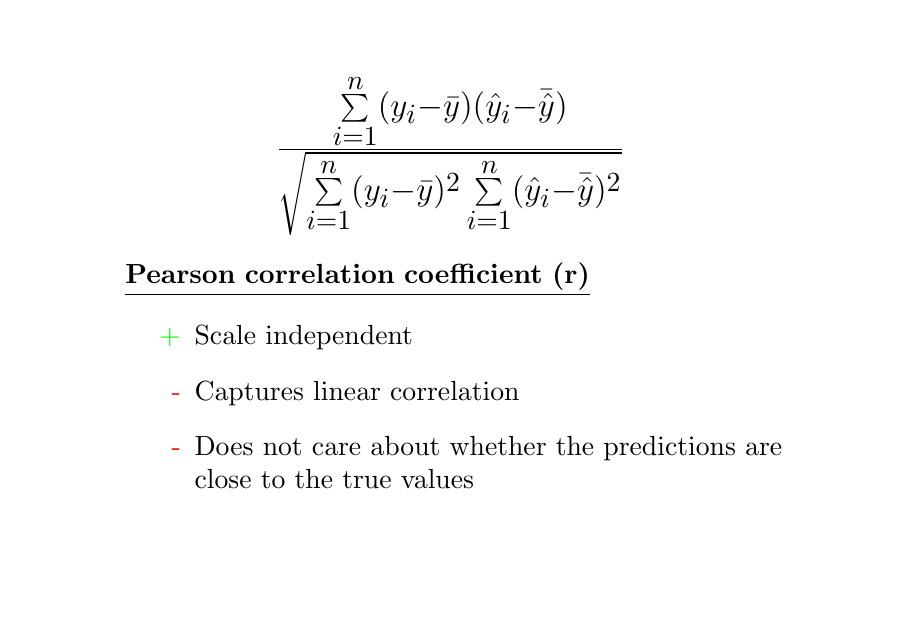
\begin{tikzpicture}
            \node[] at (0, 0) {};
            \node[] at (10.5, -7.2) {};


            \node[] at (5.25, -1.5) {
               \LARGE{$\frac{\sum\limits_{i=1}^{n} (y_i - \bar{y})(\hat{y}_i - \bar{\hat{y}})}{\sqrt{\sum\limits_{i=1}^{n} (y_i - \bar{y})^2 \sum\limits_{i=1}^{n} (\hat{y}_i - \bar{\hat{y}})^2}}$}
            };
            \node[anchor=north west, align=left, text width=8.5cm] at (1, -2.75) {
                \textbf{\underline{Pearson correlation coefficient (r)}}\\
                \begin{itemize}
                    \item[\textcolor{green}{+}] Scale independent
                    \item[\textcolor{red}{-}] Captures linear correlation
                    \item[\textcolor{red}{-}] Does not care about whether the predictions are close to the true values
                \end{itemize}
            };
        \end{tikzpicture}
    \end{frame}

    \begin{frame}[t]{Performance metrics: Regression} % r^2?
        \centering
        \begin{tikzpicture}
            \node[] at (0, 0) {};
            \node[] at (10.5, -7.2) {};


            \node[] at (5.25, -1.5) {
               \LARGE{$1 - \frac{\sum\limits_{i=1}^{n}(y_i - \hat{y}_i)^2}{\sum\limits_{i=1}^{n}(y_i - \bar{y}_i)^2}$}
            };
        \end{tikzpicture}
    \end{frame}

    \begin{frame}[t]{Performance metrics: Regression} % r^2
        \centering
        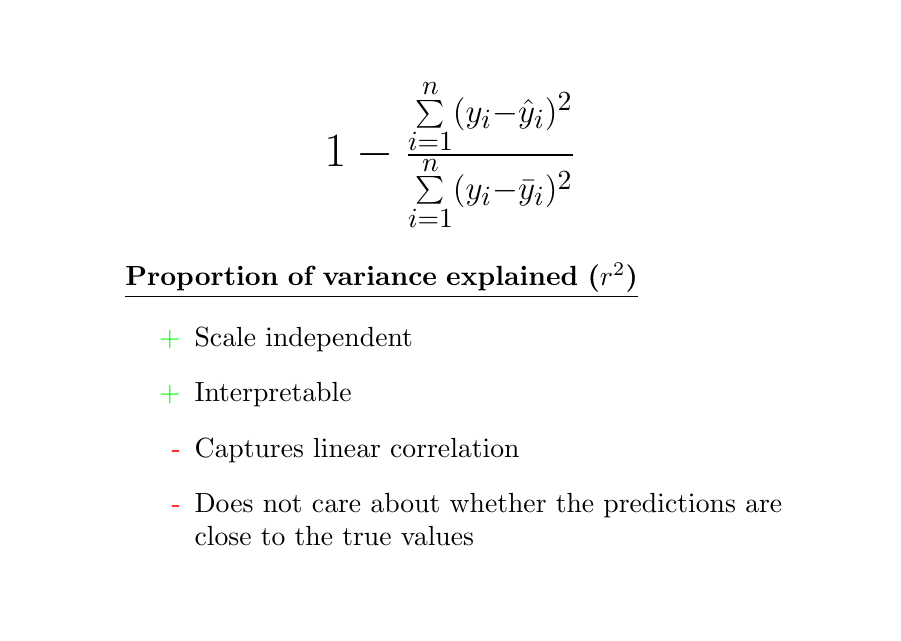
\begin{tikzpicture}
            \node[] at (0, 0) {};
            \node[] at (10.5, -7.2) {};


            \node[] at (5.25, -1.5) {
               \LARGE{$1 - \frac{\sum\limits_{i=1}^{n}(y_i - \hat{y}_i)^2}{\sum\limits_{i=1}^{n}(y_i - \bar{y}_i)^2}$}
            };
            \node[anchor=north west, align=left, text width=8.5cm] at (1, -2.75) {
                \textbf{\underline{Proportion of variance explained ($r^2$)}}\\
                \begin{itemize}
                    \item[\textcolor{green}{+}] Scale independent
                    \item[\textcolor{green}{+}] Interpretable
                    \item[\textcolor{red}{-}] Captures linear correlation
                    \item[\textcolor{red}{-}] Does not care about whether the predictions are close to the true values
                \end{itemize}
            };
        \end{tikzpicture}
    \end{frame}

    \colorlet{cases}{red}
    \colorlet{controls}{blue}

    \begin{frame}[t]{Performance metrics: Binary classification} % Groups
        \newsavebox{\casecontrolboxnine}
        \sbox{\casecontrolboxnine}{%
            \begin{tikzpicture}
                \begin{axis}[
                    height=5cm,
                    width=7cm,
                    axis lines=none,
                    ymajorticks=false,
                    xtick={0, 0.25, 0.5, 0.75, 1},
                    xlabel=\small{Prediction},
                    xmin=-0.1,
                    xmax=1.1,
                    ymin=-0.25,
                    ymax=1.25,
                    xtick pos=bottom,
                    clip=false,
                    typeset ticklabels with strut,
                    xtick={0.0, 1.0},
                    xticklabels={\small{controls}, \small{cases}},
                ]
                    \addplot[
                        only marks,
                        mark options={fill=controls}
                    ] coordinates {
                        (0.588, -0.026)
                        (0.491, 0.021)
                        (0.522, -0.042)
                        (0.450, -0.004)
                        (0.488, 0.006)
                        (0.573, 0.073)
                        (0.505, -0.060)
                        (0.554, -0.002)
                        (0.502, -0.023)
                        (0.576, -0.031)
                        (0.607, -0.018)
                        (0.544, 0.018)
                        (0.523, -0.093)
                        (0.432, -0.054)
                        (0.460, 0.085)
                        (0.479, 0.072)
                        (0.547, -0.108)
                        (0.523, -0.082)
                        (0.586, -0.049)
                        (0.527, 0.021)
                    };

                    \addplot[
                        only marks,
                        mark options={fill=cases}
                    ] coordinates {
                        (0.494, -0.047 + 1)
                        (0.526, -0.001 + 1)
                        (0.514, 0.039 + 1)
                        (0.451, -0.002 + 1)
                        (0.459, -0.077 + 1)
                        (0.533, 0.079 + 1)
                        (0.479, -0.025 + 1)
                        (0.462, 0.031 + 1)
                        (0.472, 0.038 + 1)
                        (0.462, -0.014 + 1)
                        (0.549, 0.013 + 1)
                        (0.572, 0.008 + 1)
                        (0.491, 0.022 + 1)
                        (0.501, 0.015 + 1)
                        (0.453, -0.046 + 1)
                        (0.439, -0.023 + 1)
                        (0.477, 0.007 + 1)
                        (0.446, 0.016 + 1)
                        (0.487, -0.036 + 1)
                        (0.424, 0.004 + 1)
                    };
                \end{axis}
            \end{tikzpicture}
        }

        \centering
        \begin{tikzpicture}
            \node[] at (0, 0) {};
            \node[] at (10.5, -7.2) {};

            \node[] at (5.25, -0.8) {
                \small{Cases}
            };
            \node[] at (5.25, -4.2) {
                \small{Controls}
            };

            \node[] at (5.25, -2.5) {
                \usebox{\casecontrolboxnine}
            };
        \end{tikzpicture}
    \end{frame}

    \begin{frame}[t]{Performance metrics: Binary classification} % Binary predictions
        \newsavebox{\casecontrolboxeight}
        \sbox{\casecontrolboxeight}{%
            \begin{tikzpicture}
                \begin{axis}[
                    height=5cm,
                    width=7cm,
                    axis lines=none,
                    ymajorticks=false,
                    xtick={0, 0.25, 0.5, 0.75, 1},
                    xlabel=\small{Prediction},
                    xmin=-0.1,
                    xmax=1.1,
                    ymin=-0.25,
                    ymax=1.25,
                    xtick pos=bottom,
                    clip=false,
                    typeset ticklabels with strut,
                    xtick={0.0, 1.0},
                    xticklabels={\small{controls}, \small{cases}},
                ]
                    \addplot[
                        only marks,
                        mark options={fill=controls}
                    ] coordinates {
                        (0.588 + 0.5, -0.026)
                        (0.491 + 0.5, 0.021)
                        (0.522 + 0.5, -0.042)
                        (0.450 - 0.5, -0.004)
                        (0.488 - 0.5, 0.006)
                        (0.573 - 0.5, 0.073)
                        (0.505 - 0.5, -0.060)
                        (0.554 - 0.5, -0.002)
                        (0.502 - 0.5, -0.023)
                        (0.576 - 0.5, -0.031)
                        (0.607 - 0.5, -0.018)
                        (0.544 - 0.5, 0.018)
                        (0.523 - 0.5, -0.093)
                        (0.432 - 0.5, -0.054)
                        (0.460 - 0.5, 0.085)
                        (0.479 - 0.5, 0.072)
                        (0.547 - 0.5, -0.108)
                        (0.523 - 0.5, -0.082)
                        (0.586 - 0.5, -0.049)
                        (0.527 - 0.5, 0.021)
                    };

                    \addplot[
                        only marks,
                        mark options={fill=cases}
                    ] coordinates {
                        (0.494 - 0.5, -0.047 + 1)
                        (0.526 - 0.5, -0.001 + 1)
                        (0.514 - 0.5, 0.039 + 1)
                        (0.451 + 0.5, -0.002 + 1)
                        (0.459 + 0.5, -0.077 + 1)
                        (0.533 + 0.5, 0.079 + 1)
                        (0.479 + 0.5, -0.025 + 1)
                        (0.462 + 0.5, 0.031 + 1)
                        (0.472 + 0.5, 0.038 + 1)
                        (0.462 + 0.5, -0.014 + 1)
                        (0.549 + 0.5, 0.013 + 1)
                        (0.572 + 0.5, 0.008 + 1)
                        (0.491 + 0.5, 0.022 + 1)
                        (0.501 + 0.5, 0.015 + 1)
                        (0.453 + 0.5, -0.046 + 1)
                        (0.439 + 0.5, -0.023 + 1)
                        (0.477 + 0.5, 0.007 + 1)
                        (0.446 + 0.5, 0.016 + 1)
                        (0.487 + 0.5, -0.036 + 1)
                        (0.424 + 0.5, 0.004 + 1)
                    };

                    \node[
                        align=center,
                        font=\small\linespread{0.8}\selectfont
                    ] at (axis cs: 0, 0.5) {Predicted\\controls};
                    \node[
                        align=center,
                        font=\small\linespread{0.8}\selectfont
                    ] at (axis cs: 1, 0.5) {Predicted\\cases};
                \end{axis}
            \end{tikzpicture}
        }

        \centering
        \begin{tikzpicture}
            \node[] at (0, 0) {};
            \node[] at (10.5, -7.2) {};

            \node[] at (5.25, -0.8) {
                \small{Cases}
            };
            \node[] at (5.25, -4.2) {
                \small{Controls}
            };

            \node[] at (5.25, -2.5) {
                \usebox{\casecontrolboxeight}
            };
        \end{tikzpicture}
    \end{frame}

    \begin{frame}[t]{Performance metrics: Binary classification} % Probabilities
        \newsavebox{\casecontrolboxseven}
        \sbox{\casecontrolboxseven}{%
            \begin{tikzpicture}
                \begin{axis}[
                    height=5cm,
                    width=7cm,
                    ymajorticks=false,
                    xtick={0, 0.25, 0.5, 0.75, 1},
                    xlabel=\small{Prediction},
                    xmin=-0.1,
                    xmax=1.1,
                    ymin=-0.25,
                    ymax=1.25,
                    xtick pos=bottom,
                    clip=false,
                    typeset ticklabels with strut
                ]
                    \addplot[
                        only marks,
                        mark options={fill=controls}
                    ] coordinates {
                        (0.588 - 0.5, -0.026)
                        (0.491 - 0.45, 0.021)
                        (0.522 - 0.4, -0.042)
                        (0.450 - 0.425, -0.004)
                        (0.488 - 0.375, 0.006)
                        (0.573 - 0.325, 0.073)
                        (0.505 - 0.275, -0.060)
                        (0.554 - 0.225, -0.002)
                        (0.502 - 0.35, -0.023)
                        (0.576 - 0.15, -0.031)
                        (0.607 - 0.1, -0.018)
                        (0.544 - 0.05, 0.018)
                        (0.523 - 0.0, -0.093)
                        (0.432- 0.125, -0.054)
                        (0.460 + 0.025, 0.085)
                        (0.479 + 0.075, 0.072)
                        (0.547 + 0.125, -0.108)
                        (0.523 + 0.175, -0.082)
                        (0.586+ 0.05, -0.049)
                        (0.527 + 0.2, 0.021)
                    };

                    \addplot[
                        only marks,
                        mark options={fill=cases}
                    ] coordinates {
                        (0.494 - 0.2, -0.047 + 1)
                        (0.526 - 0.15, -0.001 + 1)
                        (0.514 - 0.1, 0.039 + 1)
                        (0.451 - 0.05, -0.002 + 1)
                        (0.459 - 0.075, -0.077 + 1)
                        (0.533 + 0.025, 0.079 + 1)
                        (0.479 + 0.075, -0.025 + 1)
                        (0.462 + 0.125, 0.031 + 1)
                        (0.472 + 0.1, 0.038 + 1)
                        (0.462 + 0.15, -0.014 + 1)
                        (0.549 + 0.2, 0.013 + 1)
                        (0.572 + 0.25, 0.008 + 1)
                        (0.491 + 0.3, 0.022 + 1)
                        (0.501 + 0.325, 0.015 + 1)
                        (0.453 + 0.35, -0.046 + 1)
                        (0.439 + 0.4, -0.023 + 1)
                        (0.477 + 0.425, 0.007 + 1)
                        (0.446 + 0.45, 0.016 + 1)
                        (0.487 + 0.475, -0.036 + 1)
                        (0.424 + 0.5, 0.004 + 1)
                    };
                \end{axis}
            \end{tikzpicture}
        }

        \vspace{0.26cm}

        \centering
        \begin{tikzpicture}
            \node[] at (0, 0) {};
            \node[] at (10.5, -7.2) {};

            \node[] at (5.25, -2.5) {
                \usebox{\casecontrolboxseven}
            };
        \end{tikzpicture}
    \end{frame}

    \begin{frame}[t]{Performance metrics: Binary classification} % Threshold
        \newsavebox{\casecontrolboxsix}
        \sbox{\casecontrolboxsix}{%
            \begin{tikzpicture}
                \begin{axis}[
                    height=5cm,
                    width=7cm,
                    ymajorticks=false,
                    %xtick={0, 0.25, 0.5, 0.75, 1},
                    xlabel=\small{Prediction},
                    xtick={0.175, 0.825},
                    xticklabels={\small{controls}, \small{cases}},
                    xmin=-0.1,
                    xmax=1.1,
                    ymin=-0.25,
                    ymax=1.25,
                    xtick pos=bottom,
                    clip=false,
                    typeset ticklabels with strut
                ]
                    \addplot[
                        only marks,
                        mark options={fill=controls}
                    ] coordinates {
                        (0.588 - 0.5, -0.026)
                        (0.491 - 0.45, 0.021)
                        (0.522 - 0.4, -0.042)
                        (0.450 - 0.425, -0.004)
                        (0.488 - 0.375, 0.006)
                        (0.573 - 0.325, 0.073)
                        (0.505 - 0.275, -0.060)
                        (0.554 - 0.225, -0.002)
                        (0.502 - 0.35, -0.023)
                        (0.576 - 0.15, -0.031)
                        (0.607 - 0.1, -0.018)
                        (0.544 - 0.05, 0.018)
                        (0.523 - 0.0, -0.093)
                        (0.432- 0.125, -0.054)
                        (0.460 + 0.025, 0.085)
                        (0.479 + 0.075, 0.072)
                        (0.547 + 0.125, -0.108)
                        (0.523 + 0.175, -0.082)
                        (0.586+ 0.05, -0.049)
                        (0.527 + 0.2, 0.021)
                    };

                    \addplot[
                        only marks,
                        mark options={fill=cases}
                    ] coordinates {
                        (0.494 - 0.2, -0.047 + 1)
                        (0.526 - 0.15, -0.001 + 1)
                        (0.514 - 0.1, 0.039 + 1)
                        (0.451 - 0.05, -0.002 + 1)
                        (0.459 - 0.075, -0.077 + 1)
                        (0.533 + 0.025, 0.079 + 1)
                        (0.479 + 0.075, -0.025 + 1)
                        (0.462 + 0.125, 0.031 + 1)
                        (0.472 + 0.1, 0.038 + 1)
                        (0.462 + 0.15, -0.014 + 1)
                        (0.549 + 0.2, 0.013 + 1)
                        (0.572 + 0.25, 0.008 + 1)
                        (0.491 + 0.3, 0.022 + 1)
                        (0.501 + 0.325, 0.015 + 1)
                        (0.453 + 0.35, -0.046 + 1)
                        (0.439 + 0.4, -0.023 + 1)
                        (0.477 + 0.425, 0.007 + 1)
                        (0.446 + 0.45, 0.016 + 1)
                        (0.487 + 0.475, -0.036 + 1)
                        (0.424 + 0.5, 0.004 + 1)
                    };

                    \draw[dashed] (axis cs: 0.5, -0.25) -- (axis cs: 0.5, 1.25);
                    \node[anchor=south] at (axis cs: 0.5, 1.25) {\footnotesize{threshold}};
                \end{axis}
            \end{tikzpicture}
        }

        \centering
        \begin{tikzpicture}
            \node[] at (0, 0) {};
            \node[] at (10.5, -7.2) {};

            \node[] at (5.25, -2.5) {
                \usebox{\casecontrolboxsix}
            };
        \end{tikzpicture}
    \end{frame}

    \begin{frame}[t]{Performance metrics: Binary classification} % CM
        \newsavebox{\casecontrolboxfive}
        \sbox{\casecontrolboxfive}{%
            \begin{tikzpicture}
                \begin{axis}[
                    height=5cm,
                    width=7cm,
                    ymajorticks=false,
                    %xtick={0, 0.25, 0.5, 0.75, 1},
                    xlabel=\small{Prediction},
                    xtick={0.175, 0.825},
                    xticklabels={\small{controls}, \small{cases}},
                    xmin=-0.1,
                    xmax=1.1,
                    ymin=-0.25,
                    ymax=1.25,
                    xtick pos=bottom,
                    clip=false,
                    typeset ticklabels with strut
                ]
                    \addplot[
                        only marks,
                        mark options={fill=controls}
                    ] coordinates {
                        (0.588 - 0.5, -0.026)
                        (0.491 - 0.45, 0.021)
                        (0.522 - 0.4, -0.042)
                        (0.450 - 0.425, -0.004)
                        (0.488 - 0.375, 0.006)
                        (0.573 - 0.325, 0.073)
                        (0.505 - 0.275, -0.060)
                        (0.554 - 0.225, -0.002)
                        (0.502 - 0.35, -0.023)
                        (0.576 - 0.15, -0.031)
                        (0.607 - 0.1, -0.018)
                        (0.544 - 0.05, 0.018)
                        (0.523 - 0.0, -0.093)
                        (0.432- 0.125, -0.054)
                        (0.460 + 0.025, 0.085)
                        (0.479 + 0.075, 0.072)
                        (0.547 + 0.125, -0.108)
                        (0.523 + 0.175, -0.082)
                        (0.586+ 0.05, -0.049)
                        (0.527 + 0.2, 0.021)
                    };

                    \addplot[
                        only marks,
                        mark options={fill=cases}
                    ] coordinates {
                        (0.494 - 0.2, -0.047 + 1)
                        (0.526 - 0.15, -0.001 + 1)
                        (0.514 - 0.1, 0.039 + 1)
                        (0.451 - 0.05, -0.002 + 1)
                        (0.459 - 0.075, -0.077 + 1)
                        (0.533 + 0.025, 0.079 + 1)
                        (0.479 + 0.075, -0.025 + 1)
                        (0.462 + 0.125, 0.031 + 1)
                        (0.472 + 0.1, 0.038 + 1)
                        (0.462 + 0.15, -0.014 + 1)
                        (0.549 + 0.2, 0.013 + 1)
                        (0.572 + 0.25, 0.008 + 1)
                        (0.491 + 0.3, 0.022 + 1)
                        (0.501 + 0.325, 0.015 + 1)
                        (0.453 + 0.35, -0.046 + 1)
                        (0.439 + 0.4, -0.023 + 1)
                        (0.477 + 0.425, 0.007 + 1)
                        (0.446 + 0.45, 0.016 + 1)
                        (0.487 + 0.475, -0.036 + 1)
                        (0.424 + 0.5, 0.004 + 1)
                    };

                    \draw[dashed] (axis cs: 0.5, -0.25) -- (axis cs: 0.5, 1.25);
                    \draw[] (axis cs: -0.1, 0.5) -- (axis cs: 1.1, 0.5);
                    \node[anchor=south] at (axis cs: 0.5, 1.25) {\footnotesize{threshold}};
                \end{axis}
            \end{tikzpicture}
        }

        \centering
        \begin{tikzpicture}
            \node[] at (0, 0) {};
            \node[] at (10.5, -7.2) {};

            \node[] at (5.25, -2.5) {
                \usebox{\casecontrolboxfive}
            };

            \node[] at (5.25, -6.5) {
                \begin{tabular}{|m{0.4cm}|m{0.4cm}|}
                    \hline
                    &\\
                    \hline
                    &\\
                    \hline
                \end{tabular}
            };
        \end{tikzpicture}
    \end{frame}

    \begin{frame}[t]{Performance metrics: Binary classification} % TN
        \newsavebox{\casecontrolboxfour}
        \sbox{\casecontrolboxfour}{%
            \begin{tikzpicture}
                \begin{axis}[
                    height=5cm,
                    width=7cm,
                    ymajorticks=false,
                    %xtick={0, 0.25, 0.5, 0.75, 1},
                    xlabel=\small{Prediction},
                    xtick={0.175, 0.825},
                    xticklabels={\small{controls}, \small{cases}},
                    xmin=-0.1,
                    xmax=1.1,
                    ymin=-0.25,
                    ymax=1.25,
                    xtick pos=bottom,
                    clip=false,
                    typeset ticklabels with strut
                ]
                    \addplot[
                        only marks,
                        mark options={fill=controls}
                    ] coordinates {
                        (0.588 - 0.5, -0.026)
                        (0.491 - 0.45, 0.021)
                        (0.522 - 0.4, -0.042)
                        (0.450 - 0.425, -0.004)
                        (0.488 - 0.375, 0.006)
                        (0.573 - 0.325, 0.073)
                        (0.505 - 0.275, -0.060)
                        (0.554 - 0.225, -0.002)
                        (0.502 - 0.35, -0.023)
                        (0.576 - 0.15, -0.031)
                        (0.607 - 0.1, -0.018)
                        (0.544 - 0.05, 0.018)
                        (0.523 - 0.0, -0.093)
                        (0.432- 0.125, -0.054)
                        (0.460 + 0.025, 0.085)
                        (0.479 + 0.075, 0.072)
                        (0.547 + 0.125, -0.108)
                        (0.523 + 0.175, -0.082)
                        (0.586+ 0.05, -0.049)
                        (0.527 + 0.2, 0.021)
                    };

                    \addplot[
                        only marks,
                        mark options={fill=cases}
                    ] coordinates {
                        (0.494 - 0.2, -0.047 + 1)
                        (0.526 - 0.15, -0.001 + 1)
                        (0.514 - 0.1, 0.039 + 1)
                        (0.451 - 0.05, -0.002 + 1)
                        (0.459 - 0.075, -0.077 + 1)
                        (0.533 + 0.025, 0.079 + 1)
                        (0.479 + 0.075, -0.025 + 1)
                        (0.462 + 0.125, 0.031 + 1)
                        (0.472 + 0.1, 0.038 + 1)
                        (0.462 + 0.15, -0.014 + 1)
                        (0.549 + 0.2, 0.013 + 1)
                        (0.572 + 0.25, 0.008 + 1)
                        (0.491 + 0.3, 0.022 + 1)
                        (0.501 + 0.325, 0.015 + 1)
                        (0.453 + 0.35, -0.046 + 1)
                        (0.439 + 0.4, -0.023 + 1)
                        (0.477 + 0.425, 0.007 + 1)
                        (0.446 + 0.45, 0.016 + 1)
                        (0.487 + 0.475, -0.036 + 1)
                        (0.424 + 0.5, 0.004 + 1)
                    };

                    \draw[dashed] (axis cs: 0.5, -0.25) -- (axis cs: 0.5, 1.25);
                    \draw[] (axis cs: -0.1, 0.5) -- (axis cs: 1.1, 0.5);
                    \node[anchor=north west, inner sep=2pt] at (axis cs: -0.1, 0.5) {\footnotesize{True negatives}};
                    \node[anchor=south] at (axis cs: 0.5, 1.25) {\footnotesize{threshold}};
                \end{axis}
            \end{tikzpicture}
        }

        \centering
        \begin{tikzpicture}
            \node[] at (0, 0) {};
            \node[] at (10.5, -7.2) {};

            \node[] at (5.25, -2.5) {
                \usebox{\casecontrolboxfour}
            };

            \node[] at (5.25, -6.5) {
                \begin{tabular}{|m{0.4cm}|m{0.4cm}|}
                    \hline
                    TN&\\
                    \hline
                    &\\
                    \hline
                \end{tabular}
            };
        \end{tikzpicture}
    \end{frame}

    \begin{frame}[t]{Performance metrics: Binary classification} % TP
        \newsavebox{\casecontrolboxthree}
        \sbox{\casecontrolboxthree}{%
            \begin{tikzpicture}
                \begin{axis}[
                    height=5cm,
                    width=7cm,
                    ymajorticks=false,
                    %xtick={0, 0.25, 0.5, 0.75, 1},
                    xlabel=\small{Prediction},
                    xtick={0.175, 0.825},
                    xticklabels={\small{controls}, \small{cases}},
                    xmin=-0.1,
                    xmax=1.1,
                    ymin=-0.25,
                    ymax=1.25,
                    xtick pos=bottom,
                    clip=false,
                    typeset ticklabels with strut
                ]
                    \addplot[
                        only marks,
                        mark options={fill=controls}
                    ] coordinates {
                        (0.588 - 0.5, -0.026)
                        (0.491 - 0.45, 0.021)
                        (0.522 - 0.4, -0.042)
                        (0.450 - 0.425, -0.004)
                        (0.488 - 0.375, 0.006)
                        (0.573 - 0.325, 0.073)
                        (0.505 - 0.275, -0.060)
                        (0.554 - 0.225, -0.002)
                        (0.502 - 0.35, -0.023)
                        (0.576 - 0.15, -0.031)
                        (0.607 - 0.1, -0.018)
                        (0.544 - 0.05, 0.018)
                        (0.523 - 0.0, -0.093)
                        (0.432- 0.125, -0.054)
                        (0.460 + 0.025, 0.085)
                        (0.479 + 0.075, 0.072)
                        (0.547 + 0.125, -0.108)
                        (0.523 + 0.175, -0.082)
                        (0.586+ 0.05, -0.049)
                        (0.527 + 0.2, 0.021)
                    };

                    \addplot[
                        only marks,
                        mark options={fill=cases}
                    ] coordinates {
                        (0.494 - 0.2, -0.047 + 1)
                        (0.526 - 0.15, -0.001 + 1)
                        (0.514 - 0.1, 0.039 + 1)
                        (0.451 - 0.05, -0.002 + 1)
                        (0.459 - 0.075, -0.077 + 1)
                        (0.533 + 0.025, 0.079 + 1)
                        (0.479 + 0.075, -0.025 + 1)
                        (0.462 + 0.125, 0.031 + 1)
                        (0.472 + 0.1, 0.038 + 1)
                        (0.462 + 0.15, -0.014 + 1)
                        (0.549 + 0.2, 0.013 + 1)
                        (0.572 + 0.25, 0.008 + 1)
                        (0.491 + 0.3, 0.022 + 1)
                        (0.501 + 0.325, 0.015 + 1)
                        (0.453 + 0.35, -0.046 + 1)
                        (0.439 + 0.4, -0.023 + 1)
                        (0.477 + 0.425, 0.007 + 1)
                        (0.446 + 0.45, 0.016 + 1)
                        (0.487 + 0.475, -0.036 + 1)
                        (0.424 + 0.5, 0.004 + 1)
                    };

                    \draw[dashed] (axis cs: 0.5, -0.25) -- (axis cs: 0.5, 1.25);
                    \draw[] (axis cs: -0.1, 0.5) -- (axis cs: 1.1, 0.5);
                    \node[anchor=north west, inner sep=2pt] at (axis cs: -0.1, 0.5) {\footnotesize{True negatives}};
                    \node[anchor=south east, inner sep=2pt] at (axis cs: 1.1, 0.5) {\footnotesize{True positives}};
                    \node[anchor=south] at (axis cs: 0.5, 1.25) {\footnotesize{threshold}};
                \end{axis}
            \end{tikzpicture}
        }

        \centering
        \begin{tikzpicture}
            \node[] at (0, 0) {};
            \node[] at (10.5, -7.2) {};

            \node[] at (5.25, -2.5) {
                \usebox{\casecontrolboxthree}
            };

            \node[] at (5.25, -6.5) {
                \begin{tabular}{|m{0.4cm}|m{0.4cm}|}
                    \hline
                    TN&\\
                    \hline
                    &TP\\
                    \hline
                \end{tabular}
            };
        \end{tikzpicture}
    \end{frame}

    \begin{frame}[t]{Performance metrics: Binary classification} % FN
        \newsavebox{\casecontrolboxtwo}
        \sbox{\casecontrolboxtwo}{%
            \begin{tikzpicture}
                \begin{axis}[
                    height=5cm,
                    width=7cm,
                    ymajorticks=false,
                    %xtick={0, 0.25, 0.5, 0.75, 1},
                    xlabel=\small{Prediction},
                    xtick={0.175, 0.825},
                    xticklabels={\small{controls}, \small{cases}},
                    xmin=-0.1,
                    xmax=1.1,
                    ymin=-0.25,
                    ymax=1.25,
                    xtick pos=bottom,
                    clip=false,
                    typeset ticklabels with strut
                ]
                    \addplot[
                        only marks,
                        mark options={fill=controls}
                    ] coordinates {
                        (0.588 - 0.5, -0.026)
                        (0.491 - 0.45, 0.021)
                        (0.522 - 0.4, -0.042)
                        (0.450 - 0.425, -0.004)
                        (0.488 - 0.375, 0.006)
                        (0.573 - 0.325, 0.073)
                        (0.505 - 0.275, -0.060)
                        (0.554 - 0.225, -0.002)
                        (0.502 - 0.35, -0.023)
                        (0.576 - 0.15, -0.031)
                        (0.607 - 0.1, -0.018)
                        (0.544 - 0.05, 0.018)
                        (0.523 - 0.0, -0.093)
                        (0.432- 0.125, -0.054)
                        (0.460 + 0.025, 0.085)
                        (0.479 + 0.075, 0.072)
                        (0.547 + 0.125, -0.108)
                        (0.523 + 0.175, -0.082)
                        (0.586+ 0.05, -0.049)
                        (0.527 + 0.2, 0.021)
                    };

                    \addplot[
                        only marks,
                        mark options={fill=cases}
                    ] coordinates {
                        (0.494 - 0.2, -0.047 + 1)
                        (0.526 - 0.15, -0.001 + 1)
                        (0.514 - 0.1, 0.039 + 1)
                        (0.451 - 0.05, -0.002 + 1)
                        (0.459 - 0.075, -0.077 + 1)
                        (0.533 + 0.025, 0.079 + 1)
                        (0.479 + 0.075, -0.025 + 1)
                        (0.462 + 0.125, 0.031 + 1)
                        (0.472 + 0.1, 0.038 + 1)
                        (0.462 + 0.15, -0.014 + 1)
                        (0.549 + 0.2, 0.013 + 1)
                        (0.572 + 0.25, 0.008 + 1)
                        (0.491 + 0.3, 0.022 + 1)
                        (0.501 + 0.325, 0.015 + 1)
                        (0.453 + 0.35, -0.046 + 1)
                        (0.439 + 0.4, -0.023 + 1)
                        (0.477 + 0.425, 0.007 + 1)
                        (0.446 + 0.45, 0.016 + 1)
                        (0.487 + 0.475, -0.036 + 1)
                        (0.424 + 0.5, 0.004 + 1)
                    };

                    \draw[dashed] (axis cs: 0.5, -0.25) -- (axis cs: 0.5, 1.25);
                    \draw[] (axis cs: -0.1, 0.5) -- (axis cs: 1.1, 0.5);
                    \node[anchor=north west, inner sep=2pt] at (axis cs: -0.1, 0.5) {\footnotesize{True negatives}};
                    \node[anchor=south west, inner sep=2pt] at (axis cs: -0.1, 0.5) {\footnotesize{False negatives}};
                    \node[anchor=south east, inner sep=2pt] at (axis cs: 1.1, 0.5) {\footnotesize{True positives}};
                    \node[anchor=south] at (axis cs: 0.5, 1.25) {\footnotesize{threshold}};
                \end{axis}
            \end{tikzpicture}
        }

        \centering
        \begin{tikzpicture}
            \node[] at (0, 0) {};
            \node[] at (10.5, -7.2) {};

            \node[] at (5.25, -2.5) {
                \usebox{\casecontrolboxtwo}
            };

            \node[] at (5.25, -6.5) {
                \begin{tabular}{|m{0.4cm}|m{0.4cm}|}
                    \hline
                    TN&\\
                    \hline
                    FN&TP\\
                    \hline
                \end{tabular}
            };
        \end{tikzpicture}
    \end{frame}

    \begin{frame}[t]{Performance metrics: Binary classification} % FP
        \newsavebox{\casecontrolboxone}
        \sbox{\casecontrolboxone}{%
            \begin{tikzpicture}
                \begin{axis}[
                    height=5cm,
                    width=7cm,
                    ymajorticks=false,
                    %xtick={0, 0.25, 0.5, 0.75, 1},
                    xlabel=\small{Prediction},
                    xtick={0.175, 0.825},
                    xticklabels={\small{controls}, \small{cases}},
                    xmin=-0.1,
                    xmax=1.1,
                    ymin=-0.25,
                    ymax=1.25,
                    xtick pos=bottom,
                    clip=false,
                    typeset ticklabels with strut
                ]
                    \addplot[
                        only marks,
                        mark options={fill=controls}
                    ] coordinates {
                        (0.588 - 0.5, -0.026)
                        (0.491 - 0.45, 0.021)
                        (0.522 - 0.4, -0.042)
                        (0.450 - 0.425, -0.004)
                        (0.488 - 0.375, 0.006)
                        (0.573 - 0.325, 0.073)
                        (0.505 - 0.275, -0.060)
                        (0.554 - 0.225, -0.002)
                        (0.502 - 0.35, -0.023)
                        (0.576 - 0.15, -0.031)
                        (0.607 - 0.1, -0.018)
                        (0.544 - 0.05, 0.018)
                        (0.523 - 0.0, -0.093)
                        (0.432- 0.125, -0.054)
                        (0.460 + 0.025, 0.085)
                        (0.479 + 0.075, 0.072)
                        (0.547 + 0.125, -0.108)
                        (0.523 + 0.175, -0.082)
                        (0.586+ 0.05, -0.049)
                        (0.527 + 0.2, 0.021)
                    };

                    \addplot[
                        only marks,
                        mark options={fill=cases}
                    ] coordinates {
                        (0.494 - 0.2, -0.047 + 1)
                        (0.526 - 0.15, -0.001 + 1)
                        (0.514 - 0.1, 0.039 + 1)
                        (0.451 - 0.05, -0.002 + 1)
                        (0.459 - 0.075, -0.077 + 1)
                        (0.533 + 0.025, 0.079 + 1)
                        (0.479 + 0.075, -0.025 + 1)
                        (0.462 + 0.125, 0.031 + 1)
                        (0.472 + 0.1, 0.038 + 1)
                        (0.462 + 0.15, -0.014 + 1)
                        (0.549 + 0.2, 0.013 + 1)
                        (0.572 + 0.25, 0.008 + 1)
                        (0.491 + 0.3, 0.022 + 1)
                        (0.501 + 0.325, 0.015 + 1)
                        (0.453 + 0.35, -0.046 + 1)
                        (0.439 + 0.4, -0.023 + 1)
                        (0.477 + 0.425, 0.007 + 1)
                        (0.446 + 0.45, 0.016 + 1)
                        (0.487 + 0.475, -0.036 + 1)
                        (0.424 + 0.5, 0.004 + 1)
                    };

                    \draw[dashed] (axis cs: 0.5, -0.25) -- (axis cs: 0.5, 1.25);
                    \draw[] (axis cs: -0.1, 0.5) -- (axis cs: 1.1, 0.5);
                    \node[anchor=north west, inner sep=2pt] at (axis cs: -0.1, 0.5) {\footnotesize{True negatives}};
                    \node[anchor=south west, inner sep=2pt] at (axis cs: -0.1, 0.5) {\footnotesize{False negatives}};
                    \node[anchor=north east, inner sep=2pt] at (axis cs: 1.1, 0.5) {\footnotesize{False positives}};
                    \node[anchor=south east, inner sep=2pt] at (axis cs: 1.1, 0.5) {\footnotesize{True positives}};
                    \node[anchor=south] at (axis cs: 0.5, 1.25) {\footnotesize{threshold}};
                \end{axis}
            \end{tikzpicture}
        }

        \centering
        \begin{tikzpicture}
            \node[] at (0, 0) {};
            \node[] at (10.5, -7.2) {};

            \node[] at (5.25, -2.5) {
                \usebox{\casecontrolboxone}
            };

            \node[] at (5.25, -6.5) {
                \begin{tabular}{|m{0.4cm}|m{0.4cm}|}
                    \hline
                    TN&FP\\
                    \hline
                    FN&TP\\
                    \hline
                \end{tabular}
            };
        \end{tikzpicture}
    \end{frame}

    \begin{frame}[t]{Performance metrics: Binary classification} % Accuracy?
        \centering
        \begin{tikzpicture}
            \node[] at (0, 0) {};
            \node[] at (10.5, -7.2) {};


            \node[] at (5.25, -1.5) {
               \LARGE{$\frac{TP + TN}{TP + TN + FP + FN}$}
            };
        \end{tikzpicture}
    \end{frame}

    \begin{frame}[t]{Performance metrics: Binary classification} % Accuracy
        \centering
        
\begin{tikzpicture}
            \node[] at (0, 0) {};
            \node[] at (10.5, -7.2) {};


            \node[] at (5.25, -1.5) {
               \LARGE{$\frac{TP + TN}{TP + TN + FP + FN}$}
            };
            \node[anchor=north west, align=left, text width=8.5cm] at (1, -2.75) {
                \textbf{\underline{Accuracy}}\\
                \begin{itemize}
                    \item[\textcolor{green}{+}] \textbf{Interpretable}
                    \item[\textcolor{red}{-}] \textbf{Does not account for imbalanced classes}
                    \item[\textcolor{red}{-}] Does not account for different costs of misclassification
                \end{itemize}
            };
        \end{tikzpicture}
    \end{frame}

    \begin{frame}[t]{Performance metrics: Binary classification} % Sensitivity?
        \centering
        \begin{tikzpicture}
            \node[] at (0, 0) {};
            \node[] at (10.5, -7.2) {};


            \node[] at (5.25, -1.5) {
               \LARGE{$\frac{TP}{TP + FN}$}
            };
        \end{tikzpicture}
    \end{frame}

    \begin{frame}[t]{Performance metrics: Binary classification} % Sensitivity
        \centering
        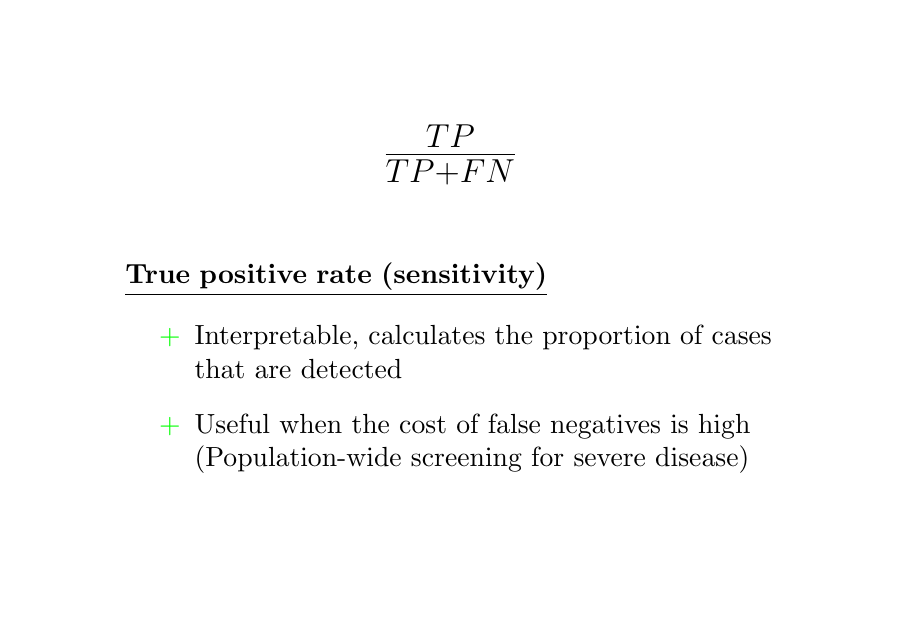
\begin{tikzpicture}
            \node[] at (0, 0) {};
            \node[] at (10.5, -7.2) {};


            \node[] at (5.25, -1.5) {
               \LARGE{$\frac{TP}{TP + FN}$}
            };
            \node[anchor=north west, align=left, text width=8.5cm] at (1, -2.75) {
                \textbf{\underline{True positive rate (sensitivity)}}\\
                \begin{itemize}
                    \item[\textcolor{green}{+}] Interpretable, calculates the proportion of cases that are detected
                    \item[\textcolor{green}{+}] Useful when the cost of false negatives is high (Population-wide screening for severe disease)
                \end{itemize}
            };
        \end{tikzpicture}
    \end{frame}

    \begin{frame}[t]{Performance metrics: Binary classification} % Specificity?
        \centering
        \begin{tikzpicture}
            \node[] at (0, 0) {};
            \node[] at (10.5, -7.2) {};


            \node[] at (5.25, -1.5) {
               \LARGE{$\frac{TN}{TN + FP}$}
            };
        \end{tikzpicture}
    \end{frame}


    \begin{frame}[t]{Performance metrics: Binary classification} % Specificity
        \centering
        
\begin{tikzpicture}
            \node[] at (0, 0) {};
            \node[] at (10.5, -7.2) {};


            \node[] at (5.25, -1.5) {
               \LARGE{$\frac{TN}{TN + FP}$}
            };
            \node[anchor=north west, align=left, text width=8.5cm] at (1, -2.75) {
                \textbf{\underline{True negative rate (specificity)}}\\
                \begin{itemize}
                    \item[\textcolor{green}{+}] Interpretable, calculates the proportion of controls that are detected
                    \item[\textcolor{green}{+}] Useful when the cost of false positives is high (Intrusive treatment of rare and mild conditions)
                \end{itemize}
            };
        \end{tikzpicture}
    \end{frame}

    \begin{frame}[t]{Performance metrics: Binary classification} % PPV?
        \centering
        \begin{tikzpicture}
            \node[] at (0, 0) {};
            \node[] at (10.5, -7.2) {};


            \node[] at (5.25, -1.5) {
               \LARGE{$\frac{TP}{TP + FP}$}
            };
        \end{tikzpicture}
    \end{frame}


    \begin{frame}[t]{Performance metrics: Binary classification} % PPV
        \centering
        
\begin{tikzpicture}
            \node[] at (0, 0) {};
            \node[] at (10.5, -7.2) {};


            \node[] at (5.25, -1.5) {
               \LARGE{$\frac{TP}{TP + FP}$}
            };
            \node[anchor=north west, align=left, text width=8.5cm] at (1, -2.75) {
                \textbf{\underline{Positive predictive value (PPV, precision)}}\\
                \begin{itemize}
                    \item[\textcolor{green}{+}] Interpretable, calculates the proportion of predicted cases that are actually cases
                    \item[\textcolor{green}{+}] Useful when the cost of false positives is high (Selection of participants for expensive clinical trials)
                \end{itemize}
            };
        \end{tikzpicture}
    \end{frame}

    \begin{frame}[t]{Performance metrics: Binary classification} % Balanced accuracy?
        \centering
        \begin{tikzpicture}
            \node[] at (0, 0) {};
            \node[] at (10.5, -7.2) {};


            \node[] at (5.25, -1.5) {
               \LARGE{$\frac{\frac{TP}{TP+FN}+\frac{TN}{TN+FP}}{2}$}
            };
        \end{tikzpicture}
    \end{frame}

    \begin{frame}[t]{Performance metrics: Binary classification} % Balanced accuracy
        \centering
        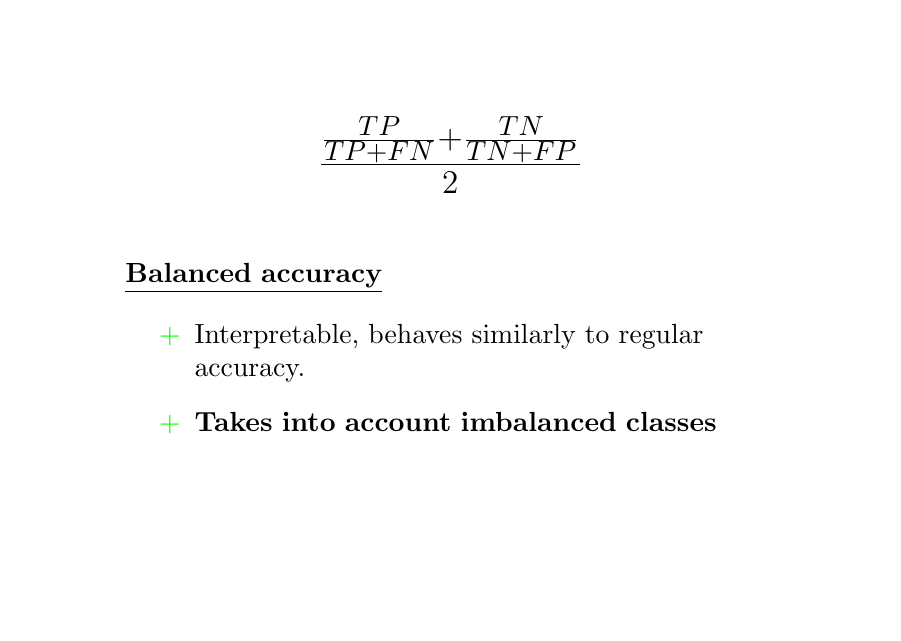
\begin{tikzpicture}
            \node[] at (0, 0) {};
            \node[] at (10.5, -7.2) {};


            \node[] at (5.25, -1.5) {
               \LARGE{$\frac{\frac{TP}{TP+FN}+\frac{TN}{TN+FP}}{2}$}
            };
            \node[anchor=north west, align=left, text width=8.5cm] at (1, -2.75) {
                \textbf{\underline{Balanced accuracy}}\\
                \begin{itemize}
                    \item[\textcolor{green}{+}] Interpretable, behaves similarly to regular accuracy.
                    \item[\textcolor{green}{+}] \textbf{Takes into account imbalanced classes}
                \end{itemize}
            };
        \end{tikzpicture}
    \end{frame}

    \begin{frame}[t]{Performance metrics: Binary classification} % Dichotomization
        \newsavebox{\casecontrolboxten}
        \sbox{\casecontrolboxten}{%
            \begin{tikzpicture}
                \begin{axis}[
                    height=3cm,
                    width=7cm,
                    ymajorticks=false,
                    xtick={0, 0.25, 0.5, 0.75, 1},
                    xlabel=\small{Prediction},
                    xmin=-0.1,
                    xmax=1.1,
                    ymin=-0.25,
                    ymax=1.25,
                    xtick pos=bottom,
                    clip=false,
                    typeset ticklabels with strut
                ]
                    \addplot[
                        only marks,
                        mark options={fill=controls}
                    ] coordinates {
                        (0.588 - 0.5, -0.026)
                        (0.491 - 0.45, 0.021)
                        (0.522 - 0.4, -0.042)
                        (0.450 - 0.425, -0.004)
                        (0.488 - 0.375, 0.006)
                        (0.573 - 0.325, 0.073)
                        (0.505 - 0.275, -0.060)
                        (0.554 - 0.225, -0.002)
                        (0.502 - 0.35, -0.023)
                        (0.576 - 0.15, -0.031)
                        (0.607 - 0.1, -0.018)
                        (0.544 - 0.05, 0.018)
                        (0.523 - 0.0, -0.093)
                        (0.432- 0.125, -0.054)
                        (0.460 + 0.025, 0.085)
                        (0.479 + 0.075, 0.072)
                        (0.547 + 0.125, -0.108)
                        (0.523 + 0.175, -0.082)
                        (0.586 + 0.05, -0.049)
                        (0.527 + 0.2, 0.021)
                    };

                    \addplot[
                        only marks,
                        mark options={fill=cases}
                    ] coordinates {
                        (0.494 - 0.2, -0.047 + 1)
                        (0.526 - 0.15, -0.001 + 1)
                        (0.514 - 0.1, 0.039 + 1)
                        (0.451 - 0.05, -0.002 + 1)
                        (0.459 - 0.075, -0.077 + 1)
                        (0.533 + 0.025, 0.079 + 1)
                        (0.479 + 0.075, -0.025 + 1)
                        (0.462 + 0.125, 0.031 + 1)
                        (0.472 + 0.1, 0.038 + 1)
                        (0.462 + 0.15, -0.014 + 1)
                        (0.549 + 0.2, 0.013 + 1)
                        (0.572 + 0.25, 0.008 + 1)
                        (0.491 + 0.3, 0.022 + 1)
                        (0.501 + 0.325, 0.015 + 1)
                        (0.453 + 0.35, -0.046 + 1)
                        (0.439 + 0.4, -0.023 + 1)
                        (0.477 + 0.425, 0.007 + 1)
                        (0.446 + 0.45, 0.016 + 1)
                        (0.487 + 0.475, -0.036 + 1)
                        (0.424 + 0.5, 0.004 + 1)
                    };
                    \draw[dashed] (axis cs: 0.5, -0.25) -- (axis cs: 0.5, 1.25);
                    \node[anchor=south] at (axis cs: 0.5, 1.25) {\footnotesize{threshold}};
                \end{axis}
            \end{tikzpicture}
        }

        \centering
        \begin{tikzpicture}
            \node[] at (0, 0) {};
            \node[] at (10.5, -7.2) {};

            \node[] at (5.25, -2) {
                \usebox{\casecontrolboxten}
            };
        \end{tikzpicture}
    \end{frame}

    \begin{frame}[t]{Performance metrics: Binary classification} % Uncalibrated
        \newsavebox{\casecontrolboxeleven}
        \sbox{\casecontrolboxeleven}{%
            \begin{tikzpicture}
                \begin{axis}[
                    height=3cm,
                    width=7cm,
                    ymajorticks=false,
                    xtick={0, 0.25, 0.5, 0.75, 1},
                    xlabel=\small{Prediction},
                    xmin=-0.1,
                    xmax=1.1,
                    ymin=-0.25,
                    ymax=1.25,
                    xtick pos=bottom,
                    clip=false,
                    typeset ticklabels with strut
                ]
                    \addplot[
                        only marks,
                        mark options={fill=controls}
                    ] coordinates {
                        ((0.588 - 0.5) * 0.4, -0.026)
                        ((0.491 - 0.45) * 0.4, 0.021)
                        ((0.522 - 0.4) * 0.4, -0.042)
                        ((0.450 - 0.425) * 0.4, -0.004)
                        ((0.488 - 0.375) * 0.4, 0.006)
                        ((0.573 - 0.325) * 0.4, 0.073)
                        ((0.505 - 0.275) * 0.4, -0.060)
                        ((0.554 - 0.225) * 0.4, -0.002)
                        ((0.502 - 0.35) * 0.4, -0.023)
                        ((0.576 - 0.15) * 0.4, -0.031)
                        ((0.607 - 0.1) * 0.4, -0.018)
                        ((0.544 - 0.05) * 0.4, 0.018)
                        ((0.523 - 0.0) * 0.4, -0.093)
                        ((0.432- 0.125) * 0.4, -0.054)
                        ((0.460 + 0.025) * 0.4, 0.085)
                        ((0.479 + 0.075) * 0.4, 0.072)
                        ((0.547 + 0.125) * 0.4, -0.108)
                        ((0.523 + 0.175) * 0.4, -0.082)
                        ((0.586 + 0.05) * 0.4, -0.049)
                        ((0.527 + 0.2) * 0.4, 0.021)
                    };

                    \addplot[
                        only marks,
                        mark options={fill=cases}
                    ] coordinates {
                        ((0.494 - 0.2) * 0.4, -0.047 + 1)
                        ((0.526 - 0.15) * 0.4, -0.001 + 1)
                        ((0.514 - 0.1) * 0.4, 0.039 + 1)
                        ((0.451 - 0.05) * 0.4, -0.002 + 1)
                        ((0.459 - 0.075) * 0.4, -0.077 + 1)
                        ((0.533 + 0.025) * 0.4, 0.079 + 1)
                        ((0.479 + 0.075) * 0.4, -0.025 + 1)
                        ((0.462 + 0.125) * 0.4, 0.031 + 1)
                        ((0.472 + 0.1) * 0.4, 0.038 + 1)
                        ((0.462 + 0.15) * 0.4, -0.014 + 1)
                        ((0.549 + 0.2) * 0.4, 0.013 + 1)
                        ((0.572 + 0.25) * 0.4, 0.008 + 1)
                        ((0.491 + 0.3) * 0.4, 0.022 + 1)
                        ((0.501 + 0.325) * 0.4, 0.015 + 1)
                        ((0.453 + 0.35) * 0.4, -0.046 + 1)
                        ((0.439 + 0.4) * 0.4, -0.023 + 1)
                        ((0.477 + 0.425) * 0.4, 0.007 + 1)
                        ((0.446 + 0.45) * 0.4, 0.016 + 1)
                        ((0.487 + 0.475) * 0.4, -0.036 + 1)
                        ((0.424 + 0.5) * 0.4, 0.004 + 1)
                    };
                    \draw[dashed] (axis cs: 0.5, -0.25) -- (axis cs: 0.5, 1.25);
                    \node[anchor=south] at (axis cs: 0.5, 1.25) {\footnotesize{threshold}};
                \end{axis}
            \end{tikzpicture}
        }

        \centering
        \begin{tikzpicture}
            \node[] at (0, 0) {};
            \node[] at (10.5, -7.2) {};

            \node[] at (5.25, -2) {
                \usebox{\casecontrolboxeleven}
            };
        \end{tikzpicture}
    \end{frame}

    \begin{frame}[t]{Performance metrics: Binary classification} % Shifted threshold
        \newsavebox{\casecontrolboxtwelve}
        \sbox{\casecontrolboxtwelve}{%
            \begin{tikzpicture}
                \begin{axis}[
                    height=3cm,
                    width=7cm,
                    ymajorticks=false,
                    xtick={0, 0.25, 0.5, 0.75, 1},
                    xlabel=\small{Prediction},
                    xmin=-0.1,
                    xmax=1.1,
                    ymin=-0.25,
                    ymax=1.25,
                    xtick pos=bottom,
                    clip=false,
                    typeset ticklabels with strut
                ]
                    \addplot[
                        only marks,
                        mark options={fill=controls}
                    ] coordinates {
                        ((0.588 - 0.5) * 0.4, -0.026)
                        ((0.491 - 0.45) * 0.4, 0.021)
                        ((0.522 - 0.4) * 0.4, -0.042)
                        ((0.450 - 0.425) * 0.4, -0.004)
                        ((0.488 - 0.375) * 0.4, 0.006)
                        ((0.573 - 0.325) * 0.4, 0.073)
                        ((0.505 - 0.275) * 0.4, -0.060)
                        ((0.554 - 0.225) * 0.4, -0.002)
                        ((0.502 - 0.35) * 0.4, -0.023)
                        ((0.576 - 0.15) * 0.4, -0.031)
                        ((0.607 - 0.1) * 0.4, -0.018)
                        ((0.544 - 0.05) * 0.4, 0.018)
                        ((0.523 - 0.0) * 0.4, -0.093)
                        ((0.432- 0.125) * 0.4, -0.054)
                        ((0.460 + 0.025) * 0.4, 0.085)
                        ((0.479 + 0.075) * 0.4, 0.072)
                        ((0.547 + 0.125) * 0.4, -0.108)
                        ((0.523 + 0.175) * 0.4, -0.082)
                        ((0.586 + 0.05) * 0.4, -0.049)
                        ((0.527 + 0.2) * 0.4, 0.021)
                    };

                    \addplot[
                        only marks,
                        mark options={fill=cases}
                    ] coordinates {
                        ((0.494 - 0.2) * 0.4, -0.047 + 1)
                        ((0.526 - 0.15) * 0.4, -0.001 + 1)
                        ((0.514 - 0.1) * 0.4, 0.039 + 1)
                        ((0.451 - 0.05) * 0.4, -0.002 + 1)
                        ((0.459 - 0.075) * 0.4, -0.077 + 1)
                        ((0.533 + 0.025) * 0.4, 0.079 + 1)
                        ((0.479 + 0.075) * 0.4, -0.025 + 1)
                        ((0.462 + 0.125) * 0.4, 0.031 + 1)
                        ((0.472 + 0.1) * 0.4, 0.038 + 1)
                        ((0.462 + 0.15) * 0.4, -0.014 + 1)
                        ((0.549 + 0.2) * 0.4, 0.013 + 1)
                        ((0.572 + 0.25) * 0.4, 0.008 + 1)
                        ((0.491 + 0.3) * 0.4, 0.022 + 1)
                        ((0.501 + 0.325) * 0.4, 0.015 + 1)
                        ((0.453 + 0.35) * 0.4, -0.046 + 1)
                        ((0.439 + 0.4) * 0.4, -0.023 + 1)
                        ((0.477 + 0.425) * 0.4, 0.007 + 1)
                        ((0.446 + 0.45) * 0.4, 0.016 + 1)
                        ((0.487 + 0.475) * 0.4, -0.036 + 1)
                        ((0.424 + 0.5) * 0.4, 0.004 + 1)
                    };
                    \draw[dashed] (axis cs: 0.2, -0.25) -- (axis cs: 0.2, 1.25);
                    \node[anchor=south] at (axis cs: 0.2, 1.25) {\footnotesize{threshold}};
                \end{axis}
            \end{tikzpicture}
        }

        \centering
        \begin{tikzpicture}
            \node[] at (0, 0) {};
            \node[] at (10.5, -7.2) {};

            \node[] at (5.25, -2) {
                \usebox{\casecontrolboxtwelve}
            };
        \end{tikzpicture}
    \end{frame}

    \begin{frame}[t]{Performance metrics: Binary classification} % Multiple threshold
        \newsavebox{\casecontrolboxthirteen}
        \sbox{\casecontrolboxthirteen}{%
            \begin{tikzpicture}
                \begin{axis}[
                    height=3cm,
                    width=7cm,
                    ymajorticks=false,
                    xtick={0, 0.25, 0.5, 0.75, 1},
                    xlabel=\small{Prediction},
                    xmin=-0.1,
                    xmax=1.1,
                    ymin=-0.25,
                    ymax=1.25,
                    xtick pos=bottom,
                    clip=false,
                    typeset ticklabels with strut
                ]
                    \addplot[
                        only marks,
                        mark options={fill=controls}
                    ] coordinates {
                        ((0.588 - 0.5) * 0.4, -0.026)
                        ((0.491 - 0.45) * 0.4, 0.021)
                        ((0.522 - 0.4) * 0.4, -0.042)
                        ((0.450 - 0.425) * 0.4, -0.004)
                        ((0.488 - 0.375) * 0.4, 0.006)
                        ((0.573 - 0.325) * 0.4, 0.073)
                        ((0.505 - 0.275) * 0.4, -0.060)
                        ((0.554 - 0.225) * 0.4, -0.002)
                        ((0.502 - 0.35) * 0.4, -0.023)
                        ((0.576 - 0.15) * 0.4, -0.031)
                        ((0.607 - 0.1) * 0.4, -0.018)
                        ((0.544 - 0.05) * 0.4, 0.018)
                        ((0.523 - 0.0) * 0.4, -0.093)
                        ((0.432- 0.125) * 0.4, -0.054)
                        ((0.460 + 0.025) * 0.4, 0.085)
                        ((0.479 + 0.075) * 0.4, 0.072)
                        ((0.547 + 0.125) * 0.4, -0.108)
                        ((0.523 + 0.175) * 0.4, -0.082)
                        ((0.586 + 0.05) * 0.4, -0.049)
                        ((0.527 + 0.2) * 0.4, 0.021)
                    };

                    \addplot[
                        only marks,
                        mark options={fill=cases}
                    ] coordinates {
                        ((0.494 - 0.2) * 0.4, -0.047 + 1)
                        ((0.526 - 0.15) * 0.4, -0.001 + 1)
                        ((0.514 - 0.1) * 0.4, 0.039 + 1)
                        ((0.451 - 0.05) * 0.4, -0.002 + 1)
                        ((0.459 - 0.075) * 0.4, -0.077 + 1)
                        ((0.533 + 0.025) * 0.4, 0.079 + 1)
                        ((0.479 + 0.075) * 0.4, -0.025 + 1)
                        ((0.462 + 0.125) * 0.4, 0.031 + 1)
                        ((0.472 + 0.1) * 0.4, 0.038 + 1)
                        ((0.462 + 0.15) * 0.4, -0.014 + 1)
                        ((0.549 + 0.2) * 0.4, 0.013 + 1)
                        ((0.572 + 0.25) * 0.4, 0.008 + 1)
                        ((0.491 + 0.3) * 0.4, 0.022 + 1)
                        ((0.501 + 0.325) * 0.4, 0.015 + 1)
                        ((0.453 + 0.35) * 0.4, -0.046 + 1)
                        ((0.439 + 0.4) * 0.4, -0.023 + 1)
                        ((0.477 + 0.425) * 0.4, 0.007 + 1)
                        ((0.446 + 0.45) * 0.4, 0.016 + 1)
                        ((0.487 + 0.475) * 0.4, -0.036 + 1)
                        ((0.424 + 0.5) * 0.4, 0.004 + 1)
                    };
                    \draw[dashed] (axis cs: 0.25, -0.25) -- (axis cs: 0.25, 1.25);
                    \draw[dashed] (axis cs: 0.5, -0.25) -- (axis cs: 0.5, 1.25);
                    \draw[dashed] (axis cs: 0.75, -0.25) -- (axis cs: 0.75, 1.25);
                \end{axis}
            \end{tikzpicture}
        }

        \centering

        \vspace{0.22cm}

        \begin{tikzpicture}
            \node[] at (0, 0) {};
            \node[] at (10.5, -7.2) {};

            \node[] at (5.25, -2) {
                \usebox{\casecontrolboxthirteen}
            };
        \end{tikzpicture}
    \end{frame}

    \begin{frame}[t]{Performance metrics: Binary classification} % ROC setup
        \newsavebox{\casecontrolboxfourteen}
        \sbox{\casecontrolboxfourteen}{%
            \begin{tikzpicture}
                \begin{axis}[
                    height=3cm,
                    width=7cm,
                    ymajorticks=false,
                    xtick={0, 0.25, 0.5, 0.75, 1},
                    xlabel=\small{Prediction},
                    xmin=-0.1,
                    xmax=1.1,
                    ymin=-0.25,
                    ymax=1.25,
                    xtick pos=bottom,
                    clip=false,
                    typeset ticklabels with strut
                ]
                    \addplot[
                        only marks,
                        mark options={fill=controls}
                    ] coordinates {
                        ((0.588 - 0.5) * 0.4, -0.026)
                        ((0.491 - 0.45) * 0.4, 0.021)
                        ((0.522 - 0.4) * 0.4, -0.042)
                        ((0.450 - 0.425) * 0.4, -0.004)
                        ((0.488 - 0.375) * 0.4, 0.006)
                        ((0.573 - 0.325) * 0.4, 0.073)
                        ((0.505 - 0.275) * 0.4, -0.060)
                        ((0.554 - 0.225) * 0.4, -0.002)
                        ((0.502 - 0.35) * 0.4, -0.023)
                        ((0.576 - 0.15) * 0.4, -0.031)
                        ((0.607 - 0.1) * 0.4, -0.018)
                        ((0.544 - 0.05) * 0.4, 0.018)
                        ((0.523 - 0.0) * 0.4, -0.093)
                        ((0.432- 0.125) * 0.4, -0.054)
                        ((0.460 + 0.025) * 0.4, 0.085)
                        ((0.479 + 0.075) * 0.4, 0.072)
                        ((0.547 + 0.125) * 0.4, -0.108)
                        ((0.523 + 0.175) * 0.4, -0.082)
                        ((0.586 + 0.05) * 0.4, -0.049)
                        ((0.527 + 0.2) * 0.4, 0.021)
                    };

                    \addplot[
                        only marks,
                        mark options={fill=cases}
                    ] coordinates {
                        ((0.494 - 0.2) * 0.4, -0.047 + 1)
                        ((0.526 - 0.15) * 0.4, -0.001 + 1)
                        ((0.514 - 0.1) * 0.4, 0.039 + 1)
                        ((0.451 - 0.05) * 0.4, -0.002 + 1)
                        ((0.459 - 0.075) * 0.4, -0.077 + 1)
                        ((0.533 + 0.025) * 0.4, 0.079 + 1)
                        ((0.479 + 0.075) * 0.4, -0.025 + 1)
                        ((0.462 + 0.125) * 0.4, 0.031 + 1)
                        ((0.472 + 0.1) * 0.4, 0.038 + 1)
                        ((0.462 + 0.15) * 0.4, -0.014 + 1)
                        ((0.549 + 0.2) * 0.4, 0.013 + 1)
                        ((0.572 + 0.25) * 0.4, 0.008 + 1)
                        ((0.491 + 0.3) * 0.4, 0.022 + 1)
                        ((0.501 + 0.325) * 0.4, 0.015 + 1)
                        ((0.453 + 0.35) * 0.4, -0.046 + 1)
                        ((0.439 + 0.4) * 0.4, -0.023 + 1)
                        ((0.477 + 0.425) * 0.4, 0.007 + 1)
                        ((0.446 + 0.45) * 0.4, 0.016 + 1)
                        ((0.487 + 0.475) * 0.4, -0.036 + 1)
                        ((0.424 + 0.5) * 0.4, 0.004 + 1)
                    };
                \end{axis}
            \end{tikzpicture}
        }

        \centering

        \vspace{0.22cm}

        \begin{tikzpicture}
            \node[] at (0, 0) {};
            \node[] at (10.5, -7.2) {};

            \node[] at (5.25, -2) {
                \usebox{\casecontrolboxfourteen}
            };

            \node[] at (5.25, -5.5) {
                \small
                \begin{tabular}{|>{\centering\arraybackslash}m{1.8cm}|>{\centering\arraybackslash}m{0.8cm}|>{\centering\arraybackslash}m{0.8cm}|}
                    \hline
                    \textbf{threshold}&\textbf{TPR}&\textbf{FPR}\\
                    \hline
                    &&\\
                    \hline
                    &&\\
                    \hline
                    &&\\
                    \hline
                    &&\\
                    \hline
                    &&\\
                    \hline
                \end{tabular}
            };
        \end{tikzpicture}
    \end{frame}

    \begin{frame}[t]{Performance metrics: Binary classification} % ROC simple thresholds
        \newsavebox{\casecontrolboxfifteen}
        \sbox{\casecontrolboxfifteen}{%
            \begin{tikzpicture}
                \begin{axis}[
                    height=3cm,
                    width=7cm,
                    ymajorticks=false,
                    xtick={0, 0.25, 0.5, 0.75, 1},
                    xlabel=\small{Prediction},
                    xmin=-0.1,
                    xmax=1.1,
                    ymin=-0.25,
                    ymax=1.25,
                    xtick pos=bottom,
                    clip=false,
                    typeset ticklabels with strut
                ]
                    \addplot[
                        only marks,
                        mark options={fill=controls}
                    ] coordinates {
                        ((0.588 - 0.5) * 0.4, -0.026)
                        ((0.491 - 0.45) * 0.4, 0.021)
                        ((0.522 - 0.4) * 0.4, -0.042)
                        ((0.450 - 0.425) * 0.4, -0.004)
                        ((0.488 - 0.375) * 0.4, 0.006)
                        ((0.573 - 0.325) * 0.4, 0.073)
                        ((0.505 - 0.275) * 0.4, -0.060)
                        ((0.554 - 0.225) * 0.4, -0.002)
                        ((0.502 - 0.35) * 0.4, -0.023)
                        ((0.576 - 0.15) * 0.4, -0.031)
                        ((0.607 - 0.1) * 0.4, -0.018)
                        ((0.544 - 0.05) * 0.4, 0.018)
                        ((0.523 - 0.0) * 0.4, -0.093)
                        ((0.432- 0.125) * 0.4, -0.054)
                        ((0.460 + 0.025) * 0.4, 0.085)
                        ((0.479 + 0.075) * 0.4, 0.072)
                        ((0.547 + 0.125) * 0.4, -0.108)
                        ((0.523 + 0.175) * 0.4, -0.082)
                        ((0.586 + 0.05) * 0.4, -0.049)
                        ((0.527 + 0.2) * 0.4, 0.021)
                    };

                    \addplot[
                        only marks,
                        mark options={fill=cases}
                    ] coordinates {
                        ((0.494 - 0.2) * 0.4, -0.047 + 1)
                        ((0.526 - 0.15) * 0.4, -0.001 + 1)
                        ((0.514 - 0.1) * 0.4, 0.039 + 1)
                        ((0.451 - 0.05) * 0.4, -0.002 + 1)
                        ((0.459 - 0.075) * 0.4, -0.077 + 1)
                        ((0.533 + 0.025) * 0.4, 0.079 + 1)
                        ((0.479 + 0.075) * 0.4, -0.025 + 1)
                        ((0.462 + 0.125) * 0.4, 0.031 + 1)
                        ((0.472 + 0.1) * 0.4, 0.038 + 1)
                        ((0.462 + 0.15) * 0.4, -0.014 + 1)
                        ((0.549 + 0.2) * 0.4, 0.013 + 1)
                        ((0.572 + 0.25) * 0.4, 0.008 + 1)
                        ((0.491 + 0.3) * 0.4, 0.022 + 1)
                        ((0.501 + 0.325) * 0.4, 0.015 + 1)
                        ((0.453 + 0.35) * 0.4, -0.046 + 1)
                        ((0.439 + 0.4) * 0.4, -0.023 + 1)
                        ((0.477 + 0.425) * 0.4, 0.007 + 1)
                        ((0.446 + 0.45) * 0.4, 0.016 + 1)
                        ((0.487 + 0.475) * 0.4, -0.036 + 1)
                        ((0.424 + 0.5) * 0.4, 0.004 + 1)
                    };
                    \draw[dashed, red, thick] (axis cs: 0, -0.25) -- (axis cs: 0, 1.25);
                    \draw[dashed, red, thick] (axis cs: 1, -0.25) -- (axis cs: 1, 1.25);
                \end{axis}
            \end{tikzpicture}
        }

        \centering

        \vspace{0.22cm}

        \begin{tikzpicture}
            \node[] at (0, 0) {};
            \node[] at (10.5, -7.2) {};

            \node[] at (5.25, -2) {
                \usebox{\casecontrolboxfifteen}
            };

            \node[] at (5.25, -5.5) {
                \small
                \begin{tabular}{|>{\centering\arraybackslash}m{1.8cm}|>{\centering\arraybackslash}m{0.8cm}|>{\centering\arraybackslash}m{0.8cm}|}
                    \hline
                    \textbf{threshold}&\textbf{TPR}&\textbf{FPR}\\
                    \hline
                    0&1&1\\
                    \hline
                    &&\\
                    \hline
                    &&\\
                    \hline
                    &&\\
                    \hline
                    1&0&0\\
                    \hline
                \end{tabular}
            };
        \end{tikzpicture}
    \end{frame}

    \begin{frame}[t]{Performance metrics: Binary classification} % ROC first threshold
        \newsavebox{\casecontrolboxsixteen}
        \sbox{\casecontrolboxsixteen}{%
            \begin{tikzpicture}
                \begin{axis}[
                    height=3cm,
                    width=7cm,
                    ymajorticks=false,
                    xtick={0, 0.25, 0.5, 0.75, 1},
                    xlabel=\small{Prediction},
                    xmin=-0.1,
                    xmax=1.1,
                    ymin=-0.25,
                    ymax=1.25,
                    xtick pos=bottom,
                    clip=false,
                    typeset ticklabels with strut
                ]
                    \addplot[
                        only marks,
                        mark options={fill=controls}
                    ] coordinates {
                        ((0.588 - 0.5) * 0.4, -0.026)
                        ((0.491 - 0.45) * 0.4, 0.021)
                        ((0.522 - 0.4) * 0.4, -0.042)
                        ((0.450 - 0.425) * 0.4, -0.004)
                        ((0.488 - 0.375) * 0.4, 0.006)
                        ((0.573 - 0.325) * 0.4, 0.073)
                        ((0.505 - 0.275) * 0.4, -0.060)
                        ((0.554 - 0.225) * 0.4, -0.002)
                        ((0.502 - 0.35) * 0.4, -0.023)
                        ((0.576 - 0.15) * 0.4, -0.031)
                        ((0.607 - 0.1) * 0.4, -0.018)
                        ((0.544 - 0.05) * 0.4, 0.018)
                        ((0.523 - 0.0) * 0.4, -0.093)
                        ((0.432- 0.125) * 0.4, -0.054)
                        ((0.460 + 0.025) * 0.4, 0.085)
                        ((0.479 + 0.075) * 0.4, 0.072)
                        ((0.547 + 0.125) * 0.4, -0.108)
                        ((0.523 + 0.175) * 0.4, -0.082)
                        ((0.586 + 0.05) * 0.4, -0.049)
                        ((0.527 + 0.2) * 0.4, 0.021)
                    };

                    \addplot[
                        only marks,
                        mark options={fill=cases}
                    ] coordinates {
                        ((0.494 - 0.2) * 0.4, -0.047 + 1)
                        ((0.526 - 0.15) * 0.4, -0.001 + 1)
                        ((0.514 - 0.1) * 0.4, 0.039 + 1)
                        ((0.451 - 0.05) * 0.4, -0.002 + 1)
                        ((0.459 - 0.075) * 0.4, -0.077 + 1)
                        ((0.533 + 0.025) * 0.4, 0.079 + 1)
                        ((0.479 + 0.075) * 0.4, -0.025 + 1)
                        ((0.462 + 0.125) * 0.4, 0.031 + 1)
                        ((0.472 + 0.1) * 0.4, 0.038 + 1)
                        ((0.462 + 0.15) * 0.4, -0.014 + 1)
                        ((0.549 + 0.2) * 0.4, 0.013 + 1)
                        ((0.572 + 0.25) * 0.4, 0.008 + 1)
                        ((0.491 + 0.3) * 0.4, 0.022 + 1)
                        ((0.501 + 0.325) * 0.4, 0.015 + 1)
                        ((0.453 + 0.35) * 0.4, -0.046 + 1)
                        ((0.439 + 0.4) * 0.4, -0.023 + 1)
                        ((0.477 + 0.425) * 0.4, 0.007 + 1)
                        ((0.446 + 0.45) * 0.4, 0.016 + 1)
                        ((0.487 + 0.475) * 0.4, -0.036 + 1)
                        ((0.424 + 0.5) * 0.4, 0.004 + 1)
                    };
                    \draw[dashed] (axis cs: 0.15, -0.25) -- (axis cs: 0.15, 1.25);
                    \draw[dashed, red, thick] (axis cs: 0, -0.25) -- (axis cs: 0, 1.25);
                    \draw[dashed, red, thick] (axis cs: 1, -0.25) -- (axis cs: 1, 1.25);
                \end{axis}
            \end{tikzpicture}
        }

        \centering

        \vspace{0.22cm}

        \begin{tikzpicture}
            \node[] at (0, 0) {};
            \node[] at (10.5, -7.2) {};

            \node[] at (5.25, -2) {
                \usebox{\casecontrolboxsixteen}
            };

            \node[] at (5.25, -5.5) {
                \small
                \begin{tabular}{|>{\centering\arraybackslash}m{1.8cm}|>{\centering\arraybackslash}m{0.8cm}|>{\centering\arraybackslash}m{0.8cm}|}
                    \hline
                    \textbf{threshold}&\textbf{TPR}&\textbf{FPR}\\
                    \hline
                    0&1&1\\
                    \hline
                    0.15&0.95&0.5\\
                    \hline
                    &&\\
                    \hline
                    &&\\
                    \hline
                    1&0&0\\
                    \hline
                \end{tabular}
            };
        \end{tikzpicture}
    \end{frame}

    \begin{frame}[t]{Performance metrics: Binary classification} % ROC all thresholds
        \newsavebox{\casecontrolboxseventeen}
        \sbox{\casecontrolboxseventeen}{%
            \begin{tikzpicture}
                \begin{axis}[
                    height=3cm,
                    width=7cm,
                    ymajorticks=false,
                    xtick={0, 0.25, 0.5, 0.75, 1},
                    xlabel=\small{Prediction},
                    xmin=-0.1,
                    xmax=1.1,
                    ymin=-0.25,
                    ymax=1.25,
                    xtick pos=bottom,
                    clip=false,
                    typeset ticklabels with strut
                ]
                    \addplot[
                        only marks,
                        mark options={fill=controls}
                    ] coordinates {
                        ((0.588 - 0.5) * 0.4, -0.026)
                        ((0.491 - 0.45) * 0.4, 0.021)
                        ((0.522 - 0.4) * 0.4, -0.042)
                        ((0.450 - 0.425) * 0.4, -0.004)
                        ((0.488 - 0.375) * 0.4, 0.006)
                        ((0.573 - 0.325) * 0.4, 0.073)
                        ((0.505 - 0.275) * 0.4, -0.060)
                        ((0.554 - 0.225) * 0.4, -0.002)
                        ((0.502 - 0.35) * 0.4, -0.023)
                        ((0.576 - 0.15) * 0.4, -0.031)
                        ((0.607 - 0.1) * 0.4, -0.018)
                        ((0.544 - 0.05) * 0.4, 0.018)
                        ((0.523 - 0.0) * 0.4, -0.093)
                        ((0.432- 0.125) * 0.4, -0.054)
                        ((0.460 + 0.025) * 0.4, 0.085)
                        ((0.479 + 0.075) * 0.4, 0.072)
                        ((0.547 + 0.125) * 0.4, -0.108)
                        ((0.523 + 0.175) * 0.4, -0.082)
                        ((0.586 + 0.05) * 0.4, -0.049)
                        ((0.527 + 0.2) * 0.4, 0.021)
                    };

                    \addplot[
                        only marks,
                        mark options={fill=cases}
                    ] coordinates {
                        ((0.494 - 0.2) * 0.4, -0.047 + 1)
                        ((0.526 - 0.15) * 0.4, -0.001 + 1)
                        ((0.514 - 0.1) * 0.4, 0.039 + 1)
                        ((0.451 - 0.05) * 0.4, -0.002 + 1)
                        ((0.459 - 0.075) * 0.4, -0.077 + 1)
                        ((0.533 + 0.025) * 0.4, 0.079 + 1)
                        ((0.479 + 0.075) * 0.4, -0.025 + 1)
                        ((0.462 + 0.125) * 0.4, 0.031 + 1)
                        ((0.472 + 0.1) * 0.4, 0.038 + 1)
                        ((0.462 + 0.15) * 0.4, -0.014 + 1)
                        ((0.549 + 0.2) * 0.4, 0.013 + 1)
                        ((0.572 + 0.25) * 0.4, 0.008 + 1)
                        ((0.491 + 0.3) * 0.4, 0.022 + 1)
                        ((0.501 + 0.325) * 0.4, 0.015 + 1)
                        ((0.453 + 0.35) * 0.4, -0.046 + 1)
                        ((0.439 + 0.4) * 0.4, -0.023 + 1)
                        ((0.477 + 0.425) * 0.4, 0.007 + 1)
                        ((0.446 + 0.45) * 0.4, 0.016 + 1)
                        ((0.487 + 0.475) * 0.4, -0.036 + 1)
                        ((0.424 + 0.5) * 0.4, 0.004 + 1)
                    };
                    \draw[dashed] (axis cs: 0.15, -0.25) -- (axis cs: 0.15, 1.25);
                    \draw[dashed] (axis cs: 0.25, -0.25) -- (axis cs: 0.25, 1.25);
                    \draw[dashed] (axis cs: 0.35, -0.25) -- (axis cs: 0.35, 1.25);
                    \draw[dashed, red, thick] (axis cs: 0, -0.25) -- (axis cs: 0, 1.25);
                    \draw[dashed, red, thick] (axis cs: 1, -0.25) -- (axis cs: 1, 1.25);
                \end{axis}
            \end{tikzpicture}
        }

        \centering

        \vspace{0.22cm}

        \begin{tikzpicture}
            \node[] at (0, 0) {};
            \node[] at (10.5, -7.2) {};

            \node[] at (5.25, -2) {
                \usebox{\casecontrolboxseventeen}
            };

            \node[] at (5.25, -5.5) {
                \small
                \begin{tabular}{|>{\centering\arraybackslash}m{1.8cm}|>{\centering\arraybackslash}m{0.8cm}|>{\centering\arraybackslash}m{0.8cm}|}
                    \hline
                    \textbf{threshold}&\textbf{TPR}&\textbf{FPR}\\
                    \hline
                    0&1&1\\
                    \hline
                    0.15&0.95&0.5\\
                    \hline
                    0.25&0.5&0.2\\
                    \hline
                    0.35&0.2&0.0\\
                    \hline
                    1&0&0\\
                    \hline
                \end{tabular}
            };
        \end{tikzpicture}
    \end{frame}

    \begin{frame}[t]{Performance metrics: Binary classification} % ROC all thresholds
        \newsavebox{\casecontrolboxeighteen}
        \sbox{\casecontrolboxeighteen}{%
            \begin{tikzpicture}
                \begin{axis}[
                    height=3cm,
                    width=7cm,
                    ymajorticks=false,
                    xtick={0, 0.25, 0.5, 0.75, 1},
                    xlabel=\small{Prediction},
                    xmin=-0.1,
                    xmax=1.1,
                    ymin=-0.25,
                    ymax=1.25,
                    xtick pos=bottom,
                    clip=false,
                    typeset ticklabels with strut
                ]
                    \addplot[
                        only marks,
                        mark options={fill=controls}
                    ] coordinates {
                        ((0.588 - 0.5) * 0.4, -0.026)
                        ((0.491 - 0.45) * 0.4, 0.021)
                        ((0.522 - 0.4) * 0.4, -0.042)
                        ((0.450 - 0.425) * 0.4, -0.004)
                        ((0.488 - 0.375) * 0.4, 0.006)
                        ((0.573 - 0.325) * 0.4, 0.073)
                        ((0.505 - 0.275) * 0.4, -0.060)
                        ((0.554 - 0.225) * 0.4, -0.002)
                        ((0.502 - 0.35) * 0.4, -0.023)
                        ((0.576 - 0.15) * 0.4, -0.031)
                        ((0.607 - 0.1) * 0.4, -0.018)
                        ((0.544 - 0.05) * 0.4, 0.018)
                        ((0.523 - 0.0) * 0.4, -0.093)
                        ((0.432- 0.125) * 0.4, -0.054)
                        ((0.460 + 0.025) * 0.4, 0.085)
                        ((0.479 + 0.075) * 0.4, 0.072)
                        ((0.547 + 0.125) * 0.4, -0.108)
                        ((0.523 + 0.175) * 0.4, -0.082)
                        ((0.586 + 0.05) * 0.4, -0.049)
                        ((0.527 + 0.2) * 0.4, 0.021)
                    };

                    \addplot[
                        only marks,
                        mark options={fill=cases}
                    ] coordinates {
                        ((0.494 - 0.2) * 0.4, -0.047 + 1)
                        ((0.526 - 0.15) * 0.4, -0.001 + 1)
                        ((0.514 - 0.1) * 0.4, 0.039 + 1)
                        ((0.451 - 0.05) * 0.4, -0.002 + 1)
                        ((0.459 - 0.075) * 0.4, -0.077 + 1)
                        ((0.533 + 0.025) * 0.4, 0.079 + 1)
                        ((0.479 + 0.075) * 0.4, -0.025 + 1)
                        ((0.462 + 0.125) * 0.4, 0.031 + 1)
                        ((0.472 + 0.1) * 0.4, 0.038 + 1)
                        ((0.462 + 0.15) * 0.4, -0.014 + 1)
                        ((0.549 + 0.2) * 0.4, 0.013 + 1)
                        ((0.572 + 0.25) * 0.4, 0.008 + 1)
                        ((0.491 + 0.3) * 0.4, 0.022 + 1)
                        ((0.501 + 0.325) * 0.4, 0.015 + 1)
                        ((0.453 + 0.35) * 0.4, -0.046 + 1)
                        ((0.439 + 0.4) * 0.4, -0.023 + 1)
                        ((0.477 + 0.425) * 0.4, 0.007 + 1)
                        ((0.446 + 0.45) * 0.4, 0.016 + 1)
                        ((0.487 + 0.475) * 0.4, -0.036 + 1)
                        ((0.424 + 0.5) * 0.4, 0.004 + 1)
                    };
                    \draw[dashed] (axis cs: 0.15, -0.25) -- (axis cs: 0.15, 1.25);
                    \draw[dashed] (axis cs: 0.25, -0.25) -- (axis cs: 0.25, 1.25);
                    \draw[dashed] (axis cs: 0.35, -0.25) -- (axis cs: 0.35, 1.25);
                    \draw[dashed, red, thick] (axis cs: 0, -0.25) -- (axis cs: 0, 1.25);
                    \draw[dashed, red, thick] (axis cs: 1, -0.25) -- (axis cs: 1, 1.25);
                \end{axis}
            \end{tikzpicture}
        }

        \centering

        \vspace{0.22cm}

        \begin{tikzpicture}
            \node[] at (0, 0) {};
            \node[] at (10.5, -7.2) {};

            \node[] at (5.25, -2) {
                \usebox{\casecontrolboxeighteen}
            };

            \node[inner sep=0pt] (table) at (5.25, -5.5) {
                \small
                \begin{tabular}{|>{\centering\arraybackslash}m{1.8cm}|>{\centering\arraybackslash}m{0.8cm}|>{\centering\arraybackslash}m{0.8cm}|}
                    \hline
                    \textbf{threshold}&\textbf{TPR}&\textbf{FPR}\\
                    \hline
                    0&1&1\\
                    \hline
                    0.15&0.95&0.5\\
                    \hline
                    0.25&0.5&0.2\\
                    \hline
                    0.35&0.2&0.0\\
                    \hline
                    1&0&0\\
                    \hline
                \end{tabular}
            };

            \node[draw=red, anchor=south east, minimum width=2.47cm, minimum height=2.29cm, inner sep=0pt, thick] at (table.south east) {};
        \end{tikzpicture}
    \end{frame}

    \begin{frame}{Performance metrics: Binary classification} % ROC points
        \centering
        \begin{tikzpicture}
            \begin{axis}[
                width=7cm,
                height=7cm,
                ylabel={True positive rate},
                xlabel={False positive rate},
                xmin=0,
                xmax=1,
                ymin=0,
                ymax=1
            ]
                \addplot[
                    only marks,
                    mark options={fill=orange!50, very thick},
                    mark size=3pt
                ] coordinates {
                    (0, 0)
                    (0, 0.2)
                    (0.2, 0.5)
                    (0.5, 0.95)
                    (1, 1)
                };
            \end{axis}
        \end{tikzpicture}
    \end{frame}

    \begin{frame}{Performance metrics: Binary classification} % ROC curve
        \centering
        \begin{tikzpicture}
            \begin{axis}[
                width=7cm,
                height=7cm,
                ylabel={True positive rate},
                xlabel={False positive rate},
                xmin=0,
                xmax=1,
                ymin=0,
                ymax=1
            ]
                \addplot[
                    very thick,
                    mark=*,
                    mark options={fill=orange!50},
                    mark size=3pt
                ] coordinates {
                    (0, 0)
                    (0, 0.2)
                    (0.2, 0.5)
                    (0.5, 0.95)
                    (1, 1)
                };
                \node[] at (axis cs: 0.27, 0.75) {ROC};
            \end{axis}
        \end{tikzpicture}
    \end{frame}

    \begin{frame}{Performance metrics: Binary classification} % ROC baseline
        \centering
        \begin{tikzpicture}
            \begin{axis}[
                width=7cm,
                height=7cm,
                ylabel={True positive rate},
                xlabel={False positive rate},
                xmin=0,
                xmax=1,
                ymin=0,
                ymax=1
            ]
                \addplot[
                    very thick,
                    mark=*,
                    mark options={fill=orange!50},
                    mark size=3pt
                ] coordinates {
                    (0, 0)
                    (0, 0.2)
                    (0.2, 0.5)
                    (0.5, 0.95)
                    (1, 1)
                };
                \node[] at (axis cs: 0.27, 0.75) {ROC};
                \addplot[dashed] coordinates {
                    (0, 0)
                    (1, 1)
                };
            \end{axis}
        \end{tikzpicture}
    \end{frame}

    \begin{frame}{Performance metrics: Binary classification} % AUC
        \centering
        \begin{tikzpicture}
            \begin{axis}[
                width=7cm,
                height=7cm,
                ylabel={True positive rate},
                xlabel={False positive rate},
                xmin=0,
                xmax=1,
                ymin=0,
                ymax=1
            ]
                \addplot[
                    very thick,
                    mark=*,
                    mark options={fill=orange!50},
                    mark size=3pt,
                    name path=roc
                ] coordinates {
                    (0, 0)
                    (0, 0.2)
                    (0.2, 0.5)
                    (0.5, 0.95)
                    (1, 1)
                };
                \node[] at (axis cs: 0.27, 0.75) {ROC};
                \addplot[dashed] coordinates {
                    (0, 0)
                    (1, 1)
                };
                \path[name path=axis] (axis cs:0,0) -- (axis cs:1,0);
                \addplot[pattern=north west lines, pattern color=red] fill between [of=roc and axis];
                \node[fill=white, draw=red] at (axis cs: 0.56, 0.45) {\textcolor{red}{AUC}};
            \end{axis}
        \end{tikzpicture}
    \end{frame}

    \begin{frame}{Performance metrics: Binary classification}
        \centering
        \begin{tikzpicture}
            \begin{axis}[
                width=7cm,
                height=7cm,
                ylabel={True positive rate},
                xlabel={False positive rate},
                xmin=0,
                xmax=1,
                ymin=0,
                ymax=1
            ]
                \addplot[
                    very thick,
                    mark=*,
                    mark options={fill=orange!50},
                    mark size=3pt
                ] coordinates {
                    (0, 0)
                    (0, 0.2)
                    (0.2, 0.5)
                    (0.5, 0.95)
                    (1, 1)
                };
                \node[] at (axis cs: 0.27, 0.75) {ROC};
                \addplot[dashed] coordinates {
                    (0, 0)
                    (1, 1)
                };
            \end{axis}
        \end{tikzpicture}
    \end{frame}

    \begin{frame}{Performance metrics: Binary classification}
        \centering
        \begin{tikzpicture}
            \begin{axis}[
                width=7cm,
                height=7cm,
                ylabel={True positive rate},
                xlabel={False positive rate},
                xmin=0,
                xmax=1,
                ymin=0,
                ymax=1
            ]
                \addplot[
                    very thick,
                    mark=*,
                    mark options={fill=orange!50},
                    mark size=3pt
                ] coordinates {
                    (0, 0)
                    (0, 0.2)
                    (0.2, 0.5)
                    (0.5, 0.95)
                    (1, 1)
                };
                \node[] at (axis cs: 0.27, 0.75) {ROC};
                \addplot[dashed] coordinates {
                    (0, 0)
                    (1, 1)
                };
                \addplot[red, dashed, thick] coordinates {
                    (0, 0.2)
                    (0.1, 0.1)
                };
                \addplot[red, dashed, thick] coordinates {
                    (0.2, 0.5)
                    (0.35, 0.35)
                };
                \addplot[red, dashed, thick] coordinates {
                    (0.5, 0.95)
                    (0.725, 0.725)
                };
            \end{axis}
        \end{tikzpicture}
    \end{frame}

    \begin{frame}{Performance metrics: Binary classification}
        \centering
        \begin{tikzpicture}
            \begin{axis}[
                width=7cm,
                height=7cm,
                ylabel={True positive rate},
                xlabel={False positive rate},
                xmin=0,
                xmax=1,
                ymin=0,
                ymax=1
            ]
                \addplot[
                    very thick,
                    mark=*,
                    mark options={fill=orange!50},
                    mark size=3pt
                ] coordinates {
                    (0, 0)
                    (0, 0.2)
                    (0.2, 0.5)
                    (0.5, 0.95)
                    (1, 1)
                };
                \node[] at (axis cs: 0.27, 0.75) {ROC};
                \addplot[dashed] coordinates {
                    (0, 0)
                    (1, 1)
                };
                \addplot[red, dashed, thick] coordinates {
                    (0, 0.2)
                    (0.1, 0.1)
                };
                \addplot[red, dashed, thick] coordinates {
                    (0.2, 0.5)
                    (0.35, 0.35)
                };
                \addplot[red, dashed, thick] coordinates {
                    (0.5, 0.95)
                    (0.725, 0.725)
                };
                \addplot[
                    very thick,
                    mark=o,
                    mark options={fill=none, draw=red},
                    mark size=5pt
                ] coordinates {
                    (0.5, 0.95)
                };
            \end{axis}
        \end{tikzpicture}
    \end{frame}

    \begin{frame}{Performance metrics: Summary}
        \begin{itemize}
            \item There is a range of metrics that can be used, each capturing a different aspect of a model's performance
            \item If possible, (it is my personal preference to) evaluate a model using a different metric than the one that was used for training
            \item It is good practice to report more than one metric
            \item For regression, MAE provides a good, intuitive summary of model performance
            \item For classification, AUC is a widely used metric that is easy to interpret, handles class imbalance (to some degree), and is not reliant on the choice of classification threshold
        \end{itemize}
    \end{frame}

    \section{Strategies for model evaluation}

    \begin{frame}{Model evaluation: Rationale}
        \textbf{\underline{Statistical inference:}}\\
        Goal: In-sample quantification
        \vspace{0.7cm}\\
        \textbf{\underline{Predictive modelling:}}\\
        Goal: Out-of-sample generalization
    \end{frame}

    \begin{frame}{Model evaluation: Validation set} % Dataset
        \centering
        \begin{tikzpicture}
            \node[] at (-4, 1) {};
            \node[] at (4, -4.5) {};
            \node[minimum height=0.5cm, minimum width=7.5cm, draw=black, fill=gray!20, label=\small{Dataset}] (full) at (0, 0) {};
        \end{tikzpicture}
    \end{frame}

    \begin{frame}{Model evaluation: Validation set} % Split
        \centering
        \begin{tikzpicture}
            \node[] at (-4, 1) {};
            \node[] at (4, -4.5) {};
            \node[minimum height=0.5cm, minimum width=7.5cm, draw=black, fill=gray!20, label=\small{Dataset}] (full) at (0, 0) {};
            \node[minimum height=0.5cm, minimum width=6cm, draw=black, fill=green!20, anchor=west, label=below:\footnotesize{Training}] (train) at (full.west) {};
            \node[minimum height=0.5cm, minimum width=1.5cm, draw=black, fill=blue!20, anchor=east, label=below:\footnotesize{Validation}] (val) at (full.east) {};
        \end{tikzpicture}
    \end{frame}

    \begin{frame}{Model evaluation: Validation set} % Training
        \centering
        \begin{tikzpicture}
            \node[] at (-4, 1) {};
            \node[] at (4, -4.5) {};
            \node[minimum height=0.5cm, minimum width=7.5cm, draw=black, fill=gray!20, label=\small{Dataset}] (full) at (0, 0) {};
            \node[minimum height=0.5cm, minimum width=6cm, draw=black, fill=green!20, anchor=west, label=below:\footnotesize{Training}] (train) at (full.west) {};
            \node[minimum height=0.5cm, minimum width=1.5cm, draw=black, fill=blue!20, anchor=east, label=below:\footnotesize{Validation}] (val) at (full.east) {};
            \node[draw=black, dashed, align=center, font=\small\linespread{0.9}\selectfont] (model) at ($ (train) - (0, 2.5) $) {Model\\fitting};

            \draw[->] ($ (train.south) - (0, 0.5) $) -- (model.north);

        \end{tikzpicture}
    \end{frame}

    \begin{frame}{Model evaluation: Validation set} % Evaluation
        \centering
        \begin{tikzpicture}
            \node[] at (-4, 1) {};
            \node[] at (4, -4.5) {};
            \node[minimum height=0.5cm, minimum width=7.5cm, draw=black, fill=gray!20, label=\small{Dataset}] (full) at (0, 0) {};
            \node[minimum height=0.5cm, minimum width=6cm, draw=black, fill=green!20, anchor=west, label=below:\footnotesize{Training}] (train) at (full.west) {};
            \node[minimum height=0.5cm, minimum width=1.5cm, draw=black, fill=blue!20, anchor=east, label=below:\footnotesize{Validation}] (val) at (full.east) {};
            \node[draw=black, dashed, align=center, font=\small\linespread{0.9}\selectfont] (model) at ($ (train) - (0, 2.5) $) {Model\\fitting};
            \node[draw=black, dashed, align=center, font=\small\linespread{0.9}\selectfont] (eval) at ($ (val) - (0, 2.5) $) {Evaluation};

            \draw[->] ($ (train.south) - (0, 0.5) $) -- (model.north);
            \draw[->] ($ (val.south) - (0, 0.5) $) -- (eval.north);

            \draw[->] (model.east) -- (eval.west) node [midway, above, sloped] {\scriptsize{Model}};

        \end{tikzpicture}
    \end{frame}

    \begin{frame}{Model evaluation: Validation set} % Performance
        \centering
        \begin{tikzpicture}
            \node[] at (-4, 1) {};
            \node[] at (4, -4.5) {};
            \node[minimum height=0.5cm, minimum width=7.5cm, draw=black, fill=gray!20, label=\small{Dataset}] (full) at (0, 0) {};
            \node[minimum height=0.5cm, minimum width=6cm, draw=black, fill=green!20, anchor=west, label=below:\footnotesize{Training}] (train) at (full.west) {};
            \node[minimum height=0.5cm, minimum width=1.5cm, draw=black, fill=blue!20, anchor=east, label=below:\footnotesize{Validation}] (val) at (full.east) {};
            \node[draw=black, dashed, align=center, font=\small\linespread{0.9}\selectfont] (model) at ($ (train) - (0, 2.5) $) {Model\\fitting};
            \node[draw=black, dashed, align=center, font=\small\linespread{0.9}\selectfont] (eval) at ($ (val) - (0, 2.5) $) {Evaluation};
            \node[align=center, font=\small\linespread{0.9}\selectfont] (score) at ($ (eval) - (0, 1.5) $) {Predictive\\performance};

            \draw[->] ($ (train.south) - (0, 0.5) $) -- (model.north);
            \draw[->] ($ (val.south) - (0, 0.5) $) -- (eval.north);

            \draw[->] ($ (eval.south) - (0, 00) $) -- (score.north);

            \draw[->] (model.east) -- (eval.west) node [midway, above, sloped] {\scriptsize{Model}};

        \end{tikzpicture}
    \end{frame}

    \begin{frame}{Model evaluation: Validation set}
        In the validation set approach we split the dataset into two subsets (commonly $\sim$80\%/20\%), use the first for training the model and the second to test its performance.
        \begin{itemize}
            \item[\textcolor{green}{+}] Accurate estimate of out-of-sample error
            \item[\textcolor{green}{+}] Simple
            \item[\textcolor{red}{-}] Variable results depending on the exact split
            \item[\textcolor{red}{-}] Only uses a subset of data for training models
            \item[\textcolor{red}{-}] Gives a point estimate of the error, without confidence intervals
        \end{itemize}
    \end{frame}

    \begin{frame}{Model evaluation: Validation set} % Performance
        \centering
        \begin{tikzpicture}
            \node[] at (-4, 1) {};
            \node[] at (4, -4.5) {};
            \node[minimum height=0.5cm, minimum width=7.5cm, draw=black, fill=gray!20, label=\small{Dataset}] (full) at (0, 0) {};
            \node[minimum height=0.5cm, minimum width=6cm, draw=black, fill=green!20, anchor=west, label=below:\footnotesize{Training}] (train) at (full.west) {};
            \node[minimum height=0.5cm, minimum width=1.5cm, draw=black, fill=blue!20, anchor=east, label=below:\footnotesize{Validation}] (val) at (full.east) {};
            \node[draw=black, dashed, align=center, font=\small\linespread{0.9}\selectfont] (model) at ($ (train) - (0, 2.5) $) {Model\\fitting};
            \node[draw=black, dashed, align=center, font=\small\linespread{0.9}\selectfont] (eval) at ($ (val) - (0, 2.5) $) {Evaluation};
            \node[align=center, font=\small\linespread{0.9}\selectfont] (score) at ($ (eval) - (0, 1.5) $) {Predictive\\performance};
            \node[align=center, font=\small\linespread{0.9}\selectfont] (trainscore) at ($ (model) - (0, 1.5) $) {Training\\performance};

            \draw[->] ($ (train.south) - (0, 0.5) $) -- (model.north);
            \draw[->] ($ (val.south) - (0, 0.5) $) -- (eval.north);

            \draw[->] ($ (eval.south) - (0, 00) $) -- (score.north);
            \draw[->] ($ (model.south) - (0, 00) $) -- (trainscore.north);

            \draw[->] (model.east) -- (eval.west) node [midway, above, sloped] {\scriptsize{Model}};

        \end{tikzpicture}
    \end{frame}

    \begin{frame}{Model evaluation: Validation set} % Performance
        \centering
        \begin{tikzpicture}
            \node[] at (-4, 1) {};
            \node[] at (4, -4.5) {};
            \node[minimum height=0.5cm, minimum width=7.5cm, draw=black, fill=gray!20, label=\small{Dataset}] (full) at (0, 0) {};
            \node[minimum height=0.5cm, minimum width=6cm, draw=black, fill=green!20, anchor=west, label=below:\footnotesize{Training}] (train) at (full.west) {};
            \node[minimum height=0.5cm, minimum width=1.5cm, draw=black, fill=blue!20, anchor=east, label=below:\footnotesize{Validation}] (val) at (full.east) {};
            \node[draw=black, dashed, align=center, font=\small\linespread{0.9}\selectfont] (model) at ($ (train) - (0, 2.5) $) {Model\\fitting};
            \node[draw=black, dashed, align=center, font=\small\linespread{0.9}\selectfont] (eval) at ($ (val) - (0, 2.5) $) {Evaluation};
            \node[align=center, font=\small\linespread{0.9}\selectfont] (score) at ($ (eval) - (0, 1.5) $) {Predictive\\performance};
            \node[align=center, font=\small\linespread{0.9}\selectfont] (trainscore) at ($ (model) - (0, 1.5) $) {Training\\performance};

            \draw[->] ($ (train.south) - (0, 0.5) $) -- (model.north);
            \draw[->] ($ (val.south) - (0, 0.5) $) -- (eval.north);

            \draw[->] ($ (eval.south) - (0, 00) $) -- (score.north);
            \draw[->] ($ (model.south) - (0, 00) $) -- (trainscore.north);

            \draw[->] (model.east) -- (eval.west) node [midway, above, sloped] {\scriptsize{Model}};

            \node[] at ($ (trainscore.east)!0.5!(score.west) $) {\textcolor{red}{$\neq$}};

        \end{tikzpicture}
    \end{frame}

    \begin{frame}{Model evaluation: Validation set} % Performance
        \centering
        \begin{tikzpicture}
            \node[] at (-4, 2) {};
            \node[] at (4, -5.5) {};
            \node[minimum height=0.5cm, minimum width=7.5cm, draw=black, fill=gray!20, label=\small{Dataset}] (full) at (0, 0) {};
            \node[minimum height=0.5cm, minimum width=6cm, draw=black, fill=green!20, anchor=west, label=below:\footnotesize{Training}] (train) at (full.west) {};
            \node[minimum height=0.5cm, minimum width=1.5cm, draw=black, fill=blue!20, anchor=east, label=below:\footnotesize{Validation}] (val) at (full.east) {};
            \node[draw=black, dashed, align=center, font=\small\linespread{0.9}\selectfont] (model) at ($ (train) - (0, 2.5) $) {Model\\fitting};
            \node[draw=black, dashed, align=center, font=\small\linespread{0.9}\selectfont] (eval) at ($ (val) - (0, 2.5) $) {Evaluation};
            \node[align=center, font=\small\linespread{0.9}\selectfont] (score) at ($ (eval) - (0, 1.5) $) {Predictive\\performance};
            \node[align=center, font=\small\linespread{0.9}\selectfont] (trainscore) at ($ (model) - (0, 1.5) $) {Training\\performance};

            \draw[->] ($ (train.south) - (0, 0.5) $) -- (model.north);
            \draw[->] ($ (val.south) - (0, 0.5) $) -- (eval.north);

            \draw[->] ($ (eval.south) - (0, 00) $) -- (score.north);
            \draw[->] ($ (model.south) - (0, 00) $) -- (trainscore.north);

            \draw[->] (model.east) -- (eval.west) node [midway, above, sloped] {\scriptsize{Model}};

            \node[] at ($ (trainscore.east)!0.5!(score.west) $) {\textcolor{red}{$\neq$}};

            \node[anchor=west, align=center, font=\small\linespread{0.9}\selectfont] (traincharacteristics) at ($ (full.west) + (0, 1) $) {Males\\>60 years};
            \node[anchor=east, align=center, font=\small\linespread{0.9}\selectfont] (valcharacteristics) at ($ (full.east) + (0, 1) $) {Females\\<40 years};

            \draw[->, densely dotted] (traincharacteristics.south) -- ($ (traincharacteristics.south) - (0, 0.3) $);
            \draw[->, densely dotted] (valcharacteristics.south) -- ($ (valcharacteristics.south) - (0, 0.3) $);

        \end{tikzpicture}
    \end{frame}

    \begin{frame}{Model evaluation: Stratification} % Definition
        \textbf{\underline{Stratification:}}\\
        Ensuring all folds of the dataset are similar with respect to some given characteristics.
    \end{frame}

    \begin{frame}{Model evaluation: Stratification} % Dataset
        \centering
        \begin{tikzpicture}
            \node[] at (-5, 1) {};
            \node[] at (5, -6) {};
            \node[minimum height=0.5cm, minimum width=7.5cm, draw=black, fill=gray!20, label=\small{Dataset}] (full) at (0, 0) {};

            \PythonInputNode{1}{(-3.5, -2.5)}{pythonnode}{7cm}{8}{
                df = ...^^J
                ^^J
                ^^J
                ^^J
                ^^J
                ^^J
            }
        \end{tikzpicture}
    \end{frame}

    \begin{frame}{Model evaluation: Stratification} % Distribution
        \centering
        \begin{tikzpicture}
            \node[] at (-5, 1) {};
            \node[] at (5, -6) {};
            \node[minimum height=0.5cm, minimum width=7.5cm, draw=black, fill=gray!20, label=\small{Dataset}] (full) at (0, 0) {};
            \node[minimum height=0.5cm, minimum width=0.375cm, draw=black, fill=red!40, anchor=west, inner sep=0pt, outer sep=0pt] (p1) at (full.west) {};
            \node[minimum height=0.5cm, minimum width=0.375cm, draw=black, fill=blue!70, anchor=west, inner sep=0pt, outer sep=0pt] (p2) at (p1.east) {};
            \node[minimum height=0.5cm, minimum width=0.375cm, draw=black, fill=blue!50, anchor=west, inner sep=0pt, outer sep=0pt] (p3) at (p2.east) {};
            \node[minimum height=0.5cm, minimum width=0.375cm, draw=black, fill=blue!30, anchor=west, inner sep=0pt, outer sep=0pt] (p4) at (p3.east) {};
            \node[minimum height=0.5cm, minimum width=0.375cm, draw=black, fill=red!80, anchor=west, inner sep=0pt, outer sep=0pt] (p5) at (p4.east) {};
            \node[minimum height=0.5cm, minimum width=0.375cm, draw=black, fill=blue!80, anchor=west, inner sep=0pt, outer sep=0pt] (p6) at (p5.east) {};
            \node[minimum height=0.5cm, minimum width=0.375cm, draw=black, fill=blue!20, anchor=west, inner sep=0pt, outer sep=0pt] (p7) at (p6.east) {};
            \node[minimum height=0.5cm, minimum width=0.375cm, draw=black, fill=red!90, anchor=west, inner sep=0pt, outer sep=0pt] (p8) at (p7.east) {};
            \node[minimum height=0.5cm, minimum width=0.375cm, draw=black, fill=blue!75, anchor=west, inner sep=0pt, outer sep=0pt] (p9) at (p8.east) {};
            \node[minimum height=0.5cm, minimum width=0.375cm, draw=black, fill=blue!85, anchor=west, inner sep=0pt, outer sep=0pt] (p10) at (p9.east) {};
            \node[minimum height=0.5cm, minimum width=0.375cm, draw=black, fill=blue!75, anchor=west, inner sep=0pt, outer sep=0pt] (p11) at (p10.east) {};
            \node[minimum height=0.5cm, minimum width=0.375cm, draw=black, fill=red!50, anchor=west, inner sep=0pt, outer sep=0pt] (p12) at (p11.east) {};
            \node[minimum height=0.5cm, minimum width=0.375cm, draw=black, fill=red!65, anchor=west, inner sep=0pt, outer sep=0pt] (p13) at (p12.east) {};
            \node[minimum height=0.5cm, minimum width=0.375cm, draw=black, fill=blue!45, anchor=west, inner sep=0pt, outer sep=0pt] (p14) at (p13.east) {};
            \node[minimum height=0.5cm, minimum width=0.375cm, draw=black, fill=red!45, anchor=west, inner sep=0pt, outer sep=0pt] (p15) at (p14.east) {};
            \node[minimum height=0.5cm, minimum width=0.375cm, draw=black, fill=blue!95, anchor=west, inner sep=0pt, outer sep=0pt] (p16) at (p15.east) {};
            \node[minimum height=0.5cm, minimum width=0.375cm, draw=black, fill=red!25, anchor=west, inner sep=0pt, outer sep=0pt] (p17) at (p16.east) {};
            \node[minimum height=0.5cm, minimum width=0.375cm, draw=black, fill=red!40, anchor=west, inner sep=0pt, outer sep=0pt] (p18) at (p17.east) {};
            \node[minimum height=0.5cm, minimum width=0.375cm, draw=black, fill=red!45, anchor=west, inner sep=0pt, outer sep=0pt] (p19) at (p18.east) {};
            \node[minimum height=0.5cm, minimum width=0.375cm, draw=black, fill=red!15, anchor=west, inner sep=0pt, outer sep=0pt] (p20) at (p19.east) {};


            \node[draw=black, fill=blue!50] (malelabel) at ($ (full.east) - (2.3, 1) $) {};
            \node[anchor=west] at (malelabel.east) {\footnotesize{Male}};
            \node[anchor=north, draw=black, fill=red!50] (femalelabel) at ($ (malelabel.south) - (0, 0.1) $) {};
            \node[anchor=west] at (femalelabel.east) {\footnotesize{Female}};

            \node[anchor=north, draw=black, shading=vertical, top color=black, bottom color=white, minimum height=0.5825cm] (agelabel) at ($ (malelabel.north) + (1.5, 0) $) {};
            \node[anchor=west] at (agelabel.east) {\footnotesize{Age}};


            \PythonInputNode{1}{(-3.5, -2.5)}{pythonnode}{7cm}{8}{
                df = ...^^J
                ^^J
                ^^J
                ^^J
                ^^J
                ^^J
            }
        \end{tikzpicture}
    \end{frame}

    \begin{frame}{Model evaluation: Stratification} % Bad split
        \centering
        \begin{tikzpicture}
            \node[] at (-5, 1) {};
            \node[] at (5, -6) {};
            \node[minimum height=0.5cm, minimum width=7.5cm, draw=black, fill=gray!20, label=\small{Dataset}] (full) at (0, 0) {};
            \node[minimum height=0.5cm, minimum width=0.375cm, draw=black, fill=red!40, anchor=west, inner sep=0pt, outer sep=0pt] (p1) at (full.west) {};
            \node[minimum height=0.5cm, minimum width=0.375cm, draw=black, fill=blue!70, anchor=west, inner sep=0pt, outer sep=0pt] (p2) at (p1.east) {};
            \node[minimum height=0.5cm, minimum width=0.375cm, draw=black, fill=blue!50, anchor=west, inner sep=0pt, outer sep=0pt] (p3) at (p2.east) {};
            \node[minimum height=0.5cm, minimum width=0.375cm, draw=black, fill=blue!30, anchor=west, inner sep=0pt, outer sep=0pt] (p4) at (p3.east) {};
            \node[minimum height=0.5cm, minimum width=0.375cm, draw=black, fill=red!80, anchor=west, inner sep=0pt, outer sep=0pt] (p5) at (p4.east) {};
            \node[minimum height=0.5cm, minimum width=0.375cm, draw=black, fill=blue!80, anchor=west, inner sep=0pt, outer sep=0pt] (p6) at (p5.east) {};
            \node[minimum height=0.5cm, minimum width=0.375cm, draw=black, fill=blue!20, anchor=west, inner sep=0pt, outer sep=0pt] (p7) at (p6.east) {};
            \node[minimum height=0.5cm, minimum width=0.375cm, draw=black, fill=red!90, anchor=west, inner sep=0pt, outer sep=0pt] (p8) at (p7.east) {};
            \node[minimum height=0.5cm, minimum width=0.375cm, draw=black, fill=blue!75, anchor=west, inner sep=0pt, outer sep=0pt] (p9) at (p8.east) {};
            \node[minimum height=0.5cm, minimum width=0.375cm, draw=black, fill=blue!85, anchor=west, inner sep=0pt, outer sep=0pt] (p10) at (p9.east) {};
            \node[minimum height=0.5cm, minimum width=0.375cm, draw=black, fill=blue!75, anchor=west, inner sep=0pt, outer sep=0pt] (p11) at (p10.east) {};
            \node[minimum height=0.5cm, minimum width=0.375cm, draw=black, fill=red!50, anchor=west, inner sep=0pt, outer sep=0pt] (p12) at (p11.east) {};
            \node[minimum height=0.5cm, minimum width=0.375cm, draw=black, fill=red!65, anchor=west, inner sep=0pt, outer sep=0pt] (p13) at (p12.east) {};
            \node[minimum height=0.5cm, minimum width=0.375cm, draw=black, fill=blue!45, anchor=west, inner sep=0pt, outer sep=0pt] (p14) at (p13.east) {};
            \node[minimum height=0.5cm, minimum width=0.375cm, draw=black, fill=red!45, anchor=west, inner sep=0pt, outer sep=0pt] (p15) at (p14.east) {};
            \node[minimum height=0.5cm, minimum width=0.375cm, draw=black, fill=blue!95, anchor=west, inner sep=0pt, outer sep=0pt] (p16) at (p15.east) {};
            \node[minimum height=0.5cm, minimum width=0.375cm, draw=black, fill=red!25, anchor=west, inner sep=0pt, outer sep=0pt] (p17) at (p16.east) {};
            \node[minimum height=0.5cm, minimum width=0.375cm, draw=black, fill=red!40, anchor=west, inner sep=0pt, outer sep=0pt] (p18) at (p17.east) {};
            \node[minimum height=0.5cm, minimum width=0.375cm, draw=black, fill=red!45, anchor=west, inner sep=0pt, outer sep=0pt] (p19) at (p18.east) {};
            \node[minimum height=0.5cm, minimum width=0.375cm, draw=black, fill=red!15, anchor=west, inner sep=0pt, outer sep=0pt] (p20) at (p19.east) {};

            \node[minimum height=0.5cm, minimum width=6cm, draw=none, fill=none, anchor=west, label=below:\footnotesize{Training}] (train) at (full.west) {};
            \node[minimum height=0.5cm, minimum width=1.5cm, draw=none, fill=none, anchor=east, label=below:\footnotesize{Validation}] (val) at (full.east) {};

            \node[draw=black, fill=blue!50] (malelabel) at ($ (full.east) - (2.3, 1) $) {};
            \node[anchor=west] at (malelabel.east) {\footnotesize{Male}};
            \node[anchor=north, draw=black, fill=red!50] (femalelabel) at ($ (malelabel.south) - (0, 0.1) $) {};
            \node[anchor=west] at (femalelabel.east) {\footnotesize{Female}};

            \node[anchor=north, draw=black, shading=vertical, top color=black, bottom color=white, minimum height=0.5825cm] (agelabel) at ($ (malelabel.north) + (1.5, 0) $) {};
            \node[anchor=west] at (agelabel.east) {\footnotesize{Age}};


            \PythonInputNode{1}{(-3.5, -2.5)}{pythonnode}{7cm}{8}{
                df = ...^^J
                ^^J
                train = df.iloc[:int(len(df) * 0.8)]^^J
                validation = df.iloc[int(len(df) * 0.8):]^^J
                ^^J
                ^^J
            }
        \end{tikzpicture}
    \end{frame}

    \begin{frame}{Model evaluation: Stratification} % Sorting
        \centering
        \begin{tikzpicture}
            \node[] at (-5, 1) {};
            \node[] at (5, -6) {};
            \node[minimum height=0.5cm, minimum width=7.5cm, draw=black, fill=gray!20, label=\small{Dataset}] (full) at (0, 0) {};
            \node[minimum height=0.5cm, minimum width=0.375cm, draw=black, fill=red!15, anchor=west, inner sep=0pt, outer sep=0pt] (p1) at (full.west) {};
            \node[minimum height=0.5cm, minimum width=0.375cm, draw=black, fill=blue!20, anchor=west, inner sep=0pt, outer sep=0pt] (p2) at (p1.east) {};
            \node[minimum height=0.5cm, minimum width=0.375cm, draw=black, fill=red!25, anchor=west, inner sep=0pt, outer sep=0pt] (p3) at (p2.east) {};
            \node[minimum height=0.5cm, minimum width=0.375cm, draw=black, fill=blue!30, anchor=west, inner sep=0pt, outer sep=0pt] (p4) at (p3.east) {};
            \node[minimum height=0.5cm, minimum width=0.375cm, draw=black, fill=red!40, anchor=west, inner sep=0pt, outer sep=0pt] (p5) at (p4.east) {};
            \node[minimum height=0.5cm, minimum width=0.375cm, draw=black, fill=blue!45, anchor=west, inner sep=0pt, outer sep=0pt] (p6) at (p5.east) {};
            \node[minimum height=0.5cm, minimum width=0.375cm, draw=black, fill=red!40, anchor=west, inner sep=0pt, outer sep=0pt] (p7) at (p6.east) {};
            \node[minimum height=0.5cm, minimum width=0.375cm, draw=black, fill=blue!50, anchor=west, inner sep=0pt, outer sep=0pt] (p8) at (p7.east) {};
            \node[minimum height=0.5cm, minimum width=0.375cm, draw=black, fill=red!45, anchor=west, inner sep=0pt, outer sep=0pt] (p9) at (p8.east) {};
            \node[minimum height=0.5cm, minimum width=0.375cm, draw=black, fill=blue!70, anchor=west, inner sep=0pt, outer sep=0pt] (p10) at (p9.east) {};
            \node[minimum height=0.5cm, minimum width=0.375cm, draw=black, fill=red!45, anchor=west, inner sep=0pt, outer sep=0pt] (p11) at (p10.east) {};
            \node[minimum height=0.5cm, minimum width=0.375cm, draw=black, fill=blue!75, anchor=west, inner sep=0pt, outer sep=0pt] (p12) at (p11.east) {};
            \node[minimum height=0.5cm, minimum width=0.375cm, draw=black, fill=red!50, anchor=west, inner sep=0pt, outer sep=0pt] (p13) at (p12.east) {};
            \node[minimum height=0.5cm, minimum width=0.375cm, draw=black, fill=blue!75, anchor=west, inner sep=0pt, outer sep=0pt] (p14) at (p13.east) {};
            \node[minimum height=0.5cm, minimum width=0.375cm, draw=black, fill=red!65, anchor=west, inner sep=0pt, outer sep=0pt] (p15) at (p14.east) {};
            \node[minimum height=0.5cm, minimum width=0.375cm, draw=black, fill=blue!80, anchor=west, inner sep=0pt, outer sep=0pt] (p16) at (p15.east) {};
            \node[minimum height=0.5cm, minimum width=0.375cm, draw=black, fill=red!80, anchor=west, inner sep=0pt, outer sep=0pt] (p17) at (p16.east) {};
            \node[minimum height=0.5cm, minimum width=0.375cm, draw=black, fill=blue!85, anchor=west, inner sep=0pt, outer sep=0pt] (p18) at (p17.east) {};
            \node[minimum height=0.5cm, minimum width=0.375cm, draw=black, fill=red!90, anchor=west, inner sep=0pt, outer sep=0pt] (p19) at (p18.east) {};
            \node[minimum height=0.5cm, minimum width=0.375cm, draw=black, fill=blue!95, anchor=west, inner sep=0pt, outer sep=0pt] (p20) at (p19.east) {};

            \node[draw=black, fill=blue!50] (malelabel) at ($ (full.east) - (2.3, 1) $) {};
            \node[anchor=west] at (malelabel.east) {\footnotesize{Male}};
            \node[anchor=north, draw=black, fill=red!50] (femalelabel) at ($ (malelabel.south) - (0, 0.1) $) {};
            \node[anchor=west] at (femalelabel.east) {\footnotesize{Female}};

            \node[anchor=north, draw=black, shading=vertical, top color=black, bottom color=white, minimum height=0.5825cm] (agelabel) at ($ (malelabel.north) + (1.5, 0) $) {};
            \node[anchor=west] at (agelabel.east) {\footnotesize{Age}};


            \PythonInputNode{1}{(-3.5, -2.5)}{pythonnode}{7cm}{8}{
                df = ...^^J
                df = df.sort_values(['sex', 'age'])^^J
                ^^J
                ^^J
                ^^J
                ^^J
            }
        \end{tikzpicture}
    \end{frame}

    \begin{frame}{Model evaluation: Stratification} % Good split
        \centering
        \begin{tikzpicture}
            \node[] at (-5, 1) {};
            \node[] at (5, -6) {};
            \node[minimum height=0.5cm, minimum width=7.5cm, draw=black, fill=gray!20, label=\small{Dataset}] (full) at (0, 0) {};
            \node[minimum height=0.5cm, minimum width=0.375cm, draw=black, fill=red!15, anchor=west, inner sep=0pt, outer sep=0pt] (p1) at (full.west) {};
            \node[minimum height=0.5cm, minimum width=0.375cm, draw=black, fill=blue!20, anchor=west, inner sep=0pt, outer sep=0pt] (p2) at (p1.east) {};
            \node[minimum height=0.5cm, minimum width=0.375cm, draw=black, fill=red!25, anchor=west, inner sep=0pt, outer sep=0pt] (p3) at (p2.east) {};
            \node[minimum height=0.5cm, minimum width=0.375cm, draw=black, fill=blue!30, anchor=west, inner sep=0pt, outer sep=0pt] (p4) at (p3.east) {};
            \node[minimum height=0.5cm, minimum width=0.375cm, draw=black, fill=red!40, anchor=west, inner sep=0pt, outer sep=0pt] (p5) at (p4.east) {};
            \node[minimum height=0.5cm, minimum width=0.375cm, draw=black, fill=blue!45, anchor=west, inner sep=0pt, outer sep=0pt] (p6) at (p5.east) {};
            \node[minimum height=0.5cm, minimum width=0.375cm, draw=black, fill=red!40, anchor=west, inner sep=0pt, outer sep=0pt] (p7) at (p6.east) {};
            \node[minimum height=0.5cm, minimum width=0.375cm, draw=black, fill=blue!50, anchor=west, inner sep=0pt, outer sep=0pt] (p8) at (p7.east) {};
            \node[minimum height=0.5cm, minimum width=0.375cm, draw=black, fill=red!45, anchor=west, inner sep=0pt, outer sep=0pt] (p9) at (p8.east) {};
            \node[minimum height=0.5cm, minimum width=0.375cm, draw=black, fill=blue!70, anchor=west, inner sep=0pt, outer sep=0pt] (p10) at (p9.east) {};
            \node[minimum height=0.5cm, minimum width=0.375cm, draw=black, fill=red!45, anchor=west, inner sep=0pt, outer sep=0pt] (p11) at (p10.east) {};
            \node[minimum height=0.5cm, minimum width=0.375cm, draw=black, fill=blue!75, anchor=west, inner sep=0pt, outer sep=0pt] (p12) at (p11.east) {};
            \node[minimum height=0.5cm, minimum width=0.375cm, draw=black, fill=red!50, anchor=west, inner sep=0pt, outer sep=0pt] (p13) at (p12.east) {};
            \node[minimum height=0.5cm, minimum width=0.375cm, draw=black, fill=blue!75, anchor=west, inner sep=0pt, outer sep=0pt] (p14) at (p13.east) {};
            \node[minimum height=0.5cm, minimum width=0.375cm, draw=black, fill=red!65, anchor=west, inner sep=0pt, outer sep=0pt] (p15) at (p14.east) {};
            \node[minimum height=0.5cm, minimum width=0.375cm, draw=black, fill=blue!80, anchor=west, inner sep=0pt, outer sep=0pt] (p16) at (p15.east) {};
            \node[minimum height=0.5cm, minimum width=0.375cm, draw=black, fill=red!80, anchor=west, inner sep=0pt, outer sep=0pt] (p17) at (p16.east) {};
            \node[minimum height=0.5cm, minimum width=0.375cm, draw=black, fill=blue!85, anchor=west, inner sep=0pt, outer sep=0pt] (p18) at (p17.east) {};
            \node[minimum height=0.5cm, minimum width=0.375cm, draw=black, fill=red!90, anchor=west, inner sep=0pt, outer sep=0pt] (p19) at (p18.east) {};
            \node[minimum height=0.5cm, minimum width=0.375cm, draw=black, fill=blue!95, anchor=west, inner sep=0pt, outer sep=0pt] (p20) at (p19.east) {};

            \node[draw=black, fill=blue!50] (malelabel) at ($ (full.east) - (2.3, 1) $) {};
            \node[anchor=west] at (malelabel.east) {\footnotesize{Male}};
            \node[anchor=north, draw=black, fill=red!50] (femalelabel) at ($ (malelabel.south) - (0, 0.1) $) {};
            \node[anchor=west] at (femalelabel.east) {\footnotesize{Female}};

            \node[anchor=north, draw=black, shading=vertical, top color=black, bottom color=white, minimum height=0.5825cm] (agelabel) at ($ (malelabel.north) + (1.5, 0) $) {};
            \node[anchor=west] at (agelabel.east) {\footnotesize{Age}};

            \draw[->, red] ($ (p1.north) + (0, 0.5) $) -- (p1);
            \draw[->, red] ($ (p6.north) + (0, 0.5) $) -- (p6);
            \draw[->, red] ($ (p11.north) + (0, 0.5) $) -- (p11);
            \draw[->, red] ($ (p16.north) + (0, 0.5) $) -- (p16);

            \PythonInputNode{1}{(-3.5, -2.5)}{pythonnode}{7cm}{8}{
                df = ...^^J
                df = df.sort_values(['sex', 'age'])^^J
                ^^J
                df['fold'] = np.arange(len(df)) \% (1 / 0.2)^^J
                train = df[df['fold'] != 0]^^J
                val = df[df['fold'] == 0]^^J
            }
        \end{tikzpicture}
    \end{frame}

    \begin{frame}{Model evaluation: Stratification} % Summary
        \textbf{\underline{Stratification:}}\\
        Ensuring all folds of the dataset are similar with respect to some given characteristics.
        \begin{itemize}
            \item Helps alleviate the risk of training performance $\gg$ validation performance
            \item \textbf{Always} stratify on target variable first
            \item Also good idea to stratify on other core characteristics, e.g. sex and age
        \end{itemize}
        \vspace{0.3cm}
        \begin{tikzpicture}
            \PythonInputNode{1}{(0, 0)}{pythonnode}{10cm}{8}{
                from sklearn.model_selection import train_test_split
            }

            \RInputNode{(0, -0.8)}{rnode}{10cm}{8}{
                library(splitstackshape)^^J
                stratified(data, columns, split)
            }
        \end{tikzpicture}
    \end{frame}

    \begin{frame}{Model evaluation: Leave-one-out cross-validation} % Dataset
        \centering
        \begin{tikzpicture}
            \node[] at (-4.5, 1) {};
            \node[] at (6.5, -5) {};

            \node[minimum height=0.5cm, minimum width=7.5cm, draw=black, fill=gray!20, label=\small{Dataset}] (full) at (0, 0) {};
        \end{tikzpicture}
    \end{frame}

    \begin{frame}{Model evaluation: Leave-one-out cross-validation} % Data points
        \centering
        \begin{tikzpicture}
            \node[] at (-4.5, 1) {};
            \node[] at (6.5, -5) {};

            \node[minimum height=0.5cm, minimum width=7.5cm, draw=black, fill=gray!20, label=\small{Dataset}] (full) at (0, 0) {};
            \node[minimum height=0.5cm, minimum width=0.375cm, draw=black, fill=gray!20, anchor=west, inner sep=0pt, outer sep=0pt] (p1) at (full.west) {};
            \node[minimum height=0.5cm, minimum width=0.375cm, draw=black, fill=gray!20, anchor=west, inner sep=0pt, outer sep=0pt] (p2) at (p1.east) {};
            \node[minimum height=0.5cm, minimum width=0.375cm, draw=black, fill=gray!20, anchor=west, inner sep=0pt, outer sep=0pt] (p3) at (p2.east) {};
            \node[minimum height=0.5cm, minimum width=0.375cm, draw=black, fill=gray!20, anchor=west, inner sep=0pt, outer sep=0pt] (p4) at (p3.east) {};
            \node[minimum height=0.5cm, minimum width=0.375cm, draw=black, fill=gray!20, anchor=west, inner sep=0pt, outer sep=0pt] (p5) at (p4.east) {};
            \node[minimum height=0.5cm, minimum width=0.375cm, draw=black, fill=gray!20, anchor=west, inner sep=0pt, outer sep=0pt] (p6) at (p5.east) {};
            \node[minimum height=0.5cm, minimum width=0.375cm, draw=black, fill=gray!20, anchor=west, inner sep=0pt, outer sep=0pt] (p7) at (p6.east) {};
            \node[minimum height=0.5cm, minimum width=0.375cm, draw=black, fill=gray!20, anchor=west, inner sep=0pt, outer sep=0pt] (p8) at (p7.east) {};
            \node[minimum height=0.5cm, minimum width=0.375cm, draw=black, fill=gray!20, anchor=west, inner sep=0pt, outer sep=0pt] (p9) at (p8.east) {};
            \node[minimum height=0.5cm, minimum width=0.375cm, draw=black, fill=gray!20, anchor=west, inner sep=0pt, outer sep=0pt] (p10) at (p9.east) {};
            \node[minimum height=0.5cm, minimum width=0.375cm, draw=black, fill=gray!20, anchor=west, inner sep=0pt, outer sep=0pt] (p11) at (p10.east) {};
            \node[minimum height=0.5cm, minimum width=0.375cm, draw=black, fill=gray!20, anchor=west, inner sep=0pt, outer sep=0pt] (p12) at (p11.east) {};
            \node[minimum height=0.5cm, minimum width=0.375cm, draw=black, fill=gray!20, anchor=west, inner sep=0pt, outer sep=0pt] (p13) at (p12.east) {};
            \node[minimum height=0.5cm, minimum width=0.375cm, draw=black, fill=gray!20, anchor=west, inner sep=0pt, outer sep=0pt] (p14) at (p13.east) {};
            \node[minimum height=0.5cm, minimum width=0.375cm, draw=black, fill=gray!20, anchor=west, inner sep=0pt, outer sep=0pt] (p15) at (p14.east) {};
            \node[minimum height=0.5cm, minimum width=0.375cm, draw=black, fill=gray!20, anchor=west, inner sep=0pt, outer sep=0pt] (p16) at (p15.east) {};
            \node[minimum height=0.5cm, minimum width=0.375cm, draw=black, fill=gray!20, anchor=west, inner sep=0pt, outer sep=0pt] (p17) at (p16.east) {};
            \node[minimum height=0.5cm, minimum width=0.375cm, draw=black, fill=gray!20, anchor=west, inner sep=0pt, outer sep=0pt] (p18) at (p17.east) {};
            \node[minimum height=0.5cm, minimum width=0.375cm, draw=black, fill=gray!20, anchor=west, inner sep=0pt, outer sep=0pt] (p19) at (p18.east) {};
            \node[minimum height=0.5cm, minimum width=0.375cm, draw=black, fill=gray!20, anchor=west, inner sep=0pt, outer sep=0pt] (p20) at (p19.east) {};
        \end{tikzpicture}
    \end{frame}

    \begin{frame}{Model evaluation: Leave-one-out cross-validation} % Split
        \centering
        \begin{tikzpicture}
            \node[] at (-4.5, 1) {};
            \node[] at (6.5, -5) {};

            \node[minimum height=0.5cm, minimum width=7.5cm, draw=black, fill=gray!20, label=\small{Dataset}] (full) at (0, 0) {};
            \node[minimum height=0.5cm, minimum width=0.375cm, draw=black, fill=green!20, anchor=west, inner sep=0pt, outer sep=0pt] (p1) at (full.west) {};
            \node[minimum height=0.5cm, minimum width=0.375cm, draw=black, fill=green!20, anchor=west, inner sep=0pt, outer sep=0pt] (p2) at (p1.east) {};
            \node[minimum height=0.5cm, minimum width=0.375cm, draw=black, fill=green!20, anchor=west, inner sep=0pt, outer sep=0pt] (p3) at (p2.east) {};
            \node[minimum height=0.5cm, minimum width=0.375cm, draw=black, fill=green!20, anchor=west, inner sep=0pt, outer sep=0pt] (p4) at (p3.east) {};
            \node[minimum height=0.5cm, minimum width=0.375cm, draw=black, fill=green!20, anchor=west, inner sep=0pt, outer sep=0pt] (p5) at (p4.east) {};
            \node[minimum height=0.5cm, minimum width=0.375cm, draw=black, fill=green!20, anchor=west, inner sep=0pt, outer sep=0pt] (p6) at (p5.east) {};
            \node[minimum height=0.5cm, minimum width=0.375cm, draw=black, fill=green!20, anchor=west, inner sep=0pt, outer sep=0pt] (p7) at (p6.east) {};
            \node[minimum height=0.5cm, minimum width=0.375cm, draw=black, fill=green!20, anchor=west, inner sep=0pt, outer sep=0pt] (p8) at (p7.east) {};
            \node[minimum height=0.5cm, minimum width=0.375cm, draw=black, fill=green!20, anchor=west, inner sep=0pt, outer sep=0pt] (p9) at (p8.east) {};
            \node[minimum height=0.5cm, minimum width=0.375cm, draw=black, fill=green!20, anchor=west, inner sep=0pt, outer sep=0pt] (p10) at (p9.east) {};
            \node[minimum height=0.5cm, minimum width=0.375cm, draw=black, fill=green!20, anchor=west, inner sep=0pt, outer sep=0pt] (p11) at (p10.east) {};
            \node[minimum height=0.5cm, minimum width=0.375cm, draw=black, fill=green!20, anchor=west, inner sep=0pt, outer sep=0pt] (p12) at (p11.east) {};
            \node[minimum height=0.5cm, minimum width=0.375cm, draw=black, fill=green!20, anchor=west, inner sep=0pt, outer sep=0pt] (p13) at (p12.east) {};
            \node[minimum height=0.5cm, minimum width=0.375cm, draw=black, fill=green!20, anchor=west, inner sep=0pt, outer sep=0pt] (p14) at (p13.east) {};
            \node[minimum height=0.5cm, minimum width=0.375cm, draw=black, fill=green!20, anchor=west, inner sep=0pt, outer sep=0pt] (p15) at (p14.east) {};
            \node[minimum height=0.5cm, minimum width=0.375cm, draw=black, fill=green!20, anchor=west, inner sep=0pt, outer sep=0pt] (p16) at (p15.east) {};
            \node[minimum height=0.5cm, minimum width=0.375cm, draw=black, fill=green!20, anchor=west, inner sep=0pt, outer sep=0pt] (p17) at (p16.east) {};
            \node[minimum height=0.5cm, minimum width=0.375cm, draw=black, fill=green!20, anchor=west, inner sep=0pt, outer sep=0pt] (p18) at (p17.east) {};
            \node[minimum height=0.5cm, minimum width=0.375cm, draw=black, fill=green!20, anchor=west, inner sep=0pt, outer sep=0pt] (p19) at (p18.east) {};
            \node[minimum height=0.5cm, minimum width=0.375cm, draw=black, fill=blue!20, anchor=west, inner sep=0pt, outer sep=0pt] (p20) at (p19.east) {};

            \node[minimum height=0.5cm, minimum width=7.125cm, draw=none, fill=none, anchor=west, label=below:\footnotesize{Training}] (train) at (full.west) {};
            \node[minimum height=0.5cm, minimum width=0.375cm, draw=none, fill=none, anchor=east, label=below:\footnotesize{Validation}] (val) at (full.east) {};
        \end{tikzpicture}
    \end{frame}

    \begin{frame}{Model evaluation: Leave-one-out cross-validation} % Single error
        \centering
        \begin{tikzpicture}
            \node[] at (-4.5, 1) {};
            \node[] at (6.5, -5) {};

            \node[minimum height=0.5cm, minimum width=7.5cm, draw=black, fill=gray!20, label=\small{Dataset}] (full) at (0, 0) {};
            \node[minimum height=0.5cm, minimum width=0.375cm, draw=black, fill=green!20, anchor=west, inner sep=0pt, outer sep=0pt] (p1) at (full.west) {};
            \node[minimum height=0.5cm, minimum width=0.375cm, draw=black, fill=green!20, anchor=west, inner sep=0pt, outer sep=0pt] (p2) at (p1.east) {};
            \node[minimum height=0.5cm, minimum width=0.375cm, draw=black, fill=green!20, anchor=west, inner sep=0pt, outer sep=0pt] (p3) at (p2.east) {};
            \node[minimum height=0.5cm, minimum width=0.375cm, draw=black, fill=green!20, anchor=west, inner sep=0pt, outer sep=0pt] (p4) at (p3.east) {};
            \node[minimum height=0.5cm, minimum width=0.375cm, draw=black, fill=green!20, anchor=west, inner sep=0pt, outer sep=0pt] (p5) at (p4.east) {};
            \node[minimum height=0.5cm, minimum width=0.375cm, draw=black, fill=green!20, anchor=west, inner sep=0pt, outer sep=0pt] (p6) at (p5.east) {};
            \node[minimum height=0.5cm, minimum width=0.375cm, draw=black, fill=green!20, anchor=west, inner sep=0pt, outer sep=0pt] (p7) at (p6.east) {};
            \node[minimum height=0.5cm, minimum width=0.375cm, draw=black, fill=green!20, anchor=west, inner sep=0pt, outer sep=0pt] (p8) at (p7.east) {};
            \node[minimum height=0.5cm, minimum width=0.375cm, draw=black, fill=green!20, anchor=west, inner sep=0pt, outer sep=0pt] (p9) at (p8.east) {};
            \node[minimum height=0.5cm, minimum width=0.375cm, draw=black, fill=green!20, anchor=west, inner sep=0pt, outer sep=0pt] (p10) at (p9.east) {};
            \node[minimum height=0.5cm, minimum width=0.375cm, draw=black, fill=green!20, anchor=west, inner sep=0pt, outer sep=0pt] (p11) at (p10.east) {};
            \node[minimum height=0.5cm, minimum width=0.375cm, draw=black, fill=green!20, anchor=west, inner sep=0pt, outer sep=0pt] (p12) at (p11.east) {};
            \node[minimum height=0.5cm, minimum width=0.375cm, draw=black, fill=green!20, anchor=west, inner sep=0pt, outer sep=0pt] (p13) at (p12.east) {};
            \node[minimum height=0.5cm, minimum width=0.375cm, draw=black, fill=green!20, anchor=west, inner sep=0pt, outer sep=0pt] (p14) at (p13.east) {};
            \node[minimum height=0.5cm, minimum width=0.375cm, draw=black, fill=green!20, anchor=west, inner sep=0pt, outer sep=0pt] (p15) at (p14.east) {};
            \node[minimum height=0.5cm, minimum width=0.375cm, draw=black, fill=green!20, anchor=west, inner sep=0pt, outer sep=0pt] (p16) at (p15.east) {};
            \node[minimum height=0.5cm, minimum width=0.375cm, draw=black, fill=green!20, anchor=west, inner sep=0pt, outer sep=0pt] (p17) at (p16.east) {};
            \node[minimum height=0.5cm, minimum width=0.375cm, draw=black, fill=green!20, anchor=west, inner sep=0pt, outer sep=0pt] (p18) at (p17.east) {};
            \node[minimum height=0.5cm, minimum width=0.375cm, draw=black, fill=green!20, anchor=west, inner sep=0pt, outer sep=0pt] (p19) at (p18.east) {};
            \node[minimum height=0.5cm, minimum width=0.375cm, draw=black, fill=blue!20, anchor=west, inner sep=0pt, outer sep=0pt] (p20) at (p19.east) {};

            \node[minimum height=0.5cm, minimum width=7.125cm, draw=none, fill=none, anchor=west, label=below:\footnotesize{Training}] (train) at (full.west) {};
            \node[minimum height=0.5cm, minimum width=0.375cm, draw=none, fill=none, anchor=east, label=below:\footnotesize{Validation}] (val) at (full.east) {};

            \node[draw=black, dashed, align=center, font=\small\linespread{0.9}\selectfont] (model) at ($ (train) - (0, 2.5) $) {Model\\fitting};
            \node[draw=black, dashed, align=center, font=\small\linespread{0.9}\selectfont] (eval) at ($ (val) - (0, 2.5) $) {Evaluation};
            \node[align=center, font=\small\linespread{0.9}\selectfont] (score) at ($ (eval) - (0, 1.5) $) {Error};

            \draw[->] ($ (train.south) - (0, 0.5) $) -- (model.north);
            \draw[->] ($ (val.south) - (0, 0.5) $) -- (eval.north);

            \draw[->] ($ (eval.south) - (0, 00) $) -- (score.north);

            \draw[->] (model.east) -- (eval.west) node [midway, above, sloped] {\scriptsize{Model}};
        \end{tikzpicture}
    \end{frame}

    \begin{frame}{Model evaluation: Leave-one-out cross-validation} % Error 1
        \centering
        \begin{tikzpicture}
            \node[] at (-4.5, 1) {};
            \node[] at (6.5, -5) {};

            \node[minimum height=0.5cm, minimum width=7.5cm, draw=black, fill=gray!20, label=\small{Dataset}] (full) at (0, 0) {};
            \node[minimum height=0.5cm, minimum width=0.375cm, draw=black, fill=green!20, anchor=west, inner sep=0pt, outer sep=0pt] (p1) at (full.west) {};
            \node[minimum height=0.5cm, minimum width=0.375cm, draw=black, fill=green!20, anchor=west, inner sep=0pt, outer sep=0pt] (p2) at (p1.east) {};
            \node[minimum height=0.5cm, minimum width=0.375cm, draw=black, fill=green!20, anchor=west, inner sep=0pt, outer sep=0pt] (p3) at (p2.east) {};
            \node[minimum height=0.5cm, minimum width=0.375cm, draw=black, fill=green!20, anchor=west, inner sep=0pt, outer sep=0pt] (p4) at (p3.east) {};
            \node[minimum height=0.5cm, minimum width=0.375cm, draw=black, fill=green!20, anchor=west, inner sep=0pt, outer sep=0pt] (p5) at (p4.east) {};
            \node[minimum height=0.5cm, minimum width=0.375cm, draw=black, fill=green!20, anchor=west, inner sep=0pt, outer sep=0pt] (p6) at (p5.east) {};
            \node[minimum height=0.5cm, minimum width=0.375cm, draw=black, fill=green!20, anchor=west, inner sep=0pt, outer sep=0pt] (p7) at (p6.east) {};
            \node[minimum height=0.5cm, minimum width=0.375cm, draw=black, fill=green!20, anchor=west, inner sep=0pt, outer sep=0pt] (p8) at (p7.east) {};
            \node[minimum height=0.5cm, minimum width=0.375cm, draw=black, fill=green!20, anchor=west, inner sep=0pt, outer sep=0pt] (p9) at (p8.east) {};
            \node[minimum height=0.5cm, minimum width=0.375cm, draw=black, fill=green!20, anchor=west, inner sep=0pt, outer sep=0pt] (p10) at (p9.east) {};
            \node[minimum height=0.5cm, minimum width=0.375cm, draw=black, fill=green!20, anchor=west, inner sep=0pt, outer sep=0pt] (p11) at (p10.east) {};
            \node[minimum height=0.5cm, minimum width=0.375cm, draw=black, fill=green!20, anchor=west, inner sep=0pt, outer sep=0pt] (p12) at (p11.east) {};
            \node[minimum height=0.5cm, minimum width=0.375cm, draw=black, fill=green!20, anchor=west, inner sep=0pt, outer sep=0pt] (p13) at (p12.east) {};
            \node[minimum height=0.5cm, minimum width=0.375cm, draw=black, fill=green!20, anchor=west, inner sep=0pt, outer sep=0pt] (p14) at (p13.east) {};
            \node[minimum height=0.5cm, minimum width=0.375cm, draw=black, fill=green!20, anchor=west, inner sep=0pt, outer sep=0pt] (p15) at (p14.east) {};
            \node[minimum height=0.5cm, minimum width=0.375cm, draw=black, fill=green!20, anchor=west, inner sep=0pt, outer sep=0pt] (p16) at (p15.east) {};
            \node[minimum height=0.5cm, minimum width=0.375cm, draw=black, fill=green!20, anchor=west, inner sep=0pt, outer sep=0pt] (p17) at (p16.east) {};
            \node[minimum height=0.5cm, minimum width=0.375cm, draw=black, fill=green!20, anchor=west, inner sep=0pt, outer sep=0pt] (p18) at (p17.east) {};
            \node[minimum height=0.5cm, minimum width=0.375cm, draw=black, fill=green!20, anchor=west, inner sep=0pt, outer sep=0pt] (p19) at (p18.east) {};
            \node[minimum height=0.5cm, minimum width=0.375cm, draw=black, fill=blue!20, anchor=west, inner sep=0pt, outer sep=0pt] (p20) at (p19.east) {};

            \node[anchor=west] (error1) at ($ (full.east) + (0.5, 0) $) {Error};
            \draw[->] (full.east) -- (error1.west);
        \end{tikzpicture}
    \end{frame}

    \begin{frame}{Model evaluation: Leave-one-out cross-validation} % Error 2
        \centering
        \begin{tikzpicture}
            \node[] at (-4.5, 1) {};
            \node[] at (6.5, -5) {};

            \node[minimum height=0.5cm, minimum width=7.5cm, draw=black, fill=gray!20, label=\small{Dataset}] (full) at (0, 0) {};
            \node[minimum height=0.5cm, minimum width=0.375cm, draw=black, fill=green!20, anchor=west, inner sep=0pt, outer sep=0pt] (p1) at (full.west) {};
            \node[minimum height=0.5cm, minimum width=0.375cm, draw=black, fill=green!20, anchor=west, inner sep=0pt, outer sep=0pt] (p2) at (p1.east) {};
            \node[minimum height=0.5cm, minimum width=0.375cm, draw=black, fill=green!20, anchor=west, inner sep=0pt, outer sep=0pt] (p3) at (p2.east) {};
            \node[minimum height=0.5cm, minimum width=0.375cm, draw=black, fill=green!20, anchor=west, inner sep=0pt, outer sep=0pt] (p4) at (p3.east) {};
            \node[minimum height=0.5cm, minimum width=0.375cm, draw=black, fill=green!20, anchor=west, inner sep=0pt, outer sep=0pt] (p5) at (p4.east) {};
            \node[minimum height=0.5cm, minimum width=0.375cm, draw=black, fill=green!20, anchor=west, inner sep=0pt, outer sep=0pt] (p6) at (p5.east) {};
            \node[minimum height=0.5cm, minimum width=0.375cm, draw=black, fill=green!20, anchor=west, inner sep=0pt, outer sep=0pt] (p7) at (p6.east) {};
            \node[minimum height=0.5cm, minimum width=0.375cm, draw=black, fill=green!20, anchor=west, inner sep=0pt, outer sep=0pt] (p8) at (p7.east) {};
            \node[minimum height=0.5cm, minimum width=0.375cm, draw=black, fill=green!20, anchor=west, inner sep=0pt, outer sep=0pt] (p9) at (p8.east) {};
            \node[minimum height=0.5cm, minimum width=0.375cm, draw=black, fill=green!20, anchor=west, inner sep=0pt, outer sep=0pt] (p10) at (p9.east) {};
            \node[minimum height=0.5cm, minimum width=0.375cm, draw=black, fill=green!20, anchor=west, inner sep=0pt, outer sep=0pt] (p11) at (p10.east) {};
            \node[minimum height=0.5cm, minimum width=0.375cm, draw=black, fill=green!20, anchor=west, inner sep=0pt, outer sep=0pt] (p12) at (p11.east) {};
            \node[minimum height=0.5cm, minimum width=0.375cm, draw=black, fill=green!20, anchor=west, inner sep=0pt, outer sep=0pt] (p13) at (p12.east) {};
            \node[minimum height=0.5cm, minimum width=0.375cm, draw=black, fill=green!20, anchor=west, inner sep=0pt, outer sep=0pt] (p14) at (p13.east) {};
            \node[minimum height=0.5cm, minimum width=0.375cm, draw=black, fill=green!20, anchor=west, inner sep=0pt, outer sep=0pt] (p15) at (p14.east) {};
            \node[minimum height=0.5cm, minimum width=0.375cm, draw=black, fill=green!20, anchor=west, inner sep=0pt, outer sep=0pt] (p16) at (p15.east) {};
            \node[minimum height=0.5cm, minimum width=0.375cm, draw=black, fill=green!20, anchor=west, inner sep=0pt, outer sep=0pt] (p17) at (p16.east) {};
            \node[minimum height=0.5cm, minimum width=0.375cm, draw=black, fill=green!20, anchor=west, inner sep=0pt, outer sep=0pt] (p18) at (p17.east) {};
            \node[minimum height=0.5cm, minimum width=0.375cm, draw=black, fill=green!20, anchor=west, inner sep=0pt, outer sep=0pt] (p19) at (p18.east) {};
            \node[minimum height=0.5cm, minimum width=0.375cm, draw=black, fill=blue!20, anchor=west, inner sep=0pt, outer sep=0pt] (p20) at (p19.east) {};

            \node[anchor=west] (error1) at ($ (full.east) + (0.5, 0) $) {Error};
            \draw[->] (full.east) -- (error1.west);

            \node[minimum height=0.5cm, minimum width=7.5cm, draw=black, fill=gray!20] (full2) at (0, -1) {};
            \node[minimum height=0.5cm, minimum width=0.375cm, draw=black, fill=green!20, anchor=west, inner sep=0pt, outer sep=0pt] (p21) at (full2.west) {};
            \node[minimum height=0.5cm, minimum width=0.375cm, draw=black, fill=green!20, anchor=west, inner sep=0pt, outer sep=0pt] (p22) at (p21.east) {};
            \node[minimum height=0.5cm, minimum width=0.375cm, draw=black, fill=green!20, anchor=west, inner sep=0pt, outer sep=0pt] (p23) at (p22.east) {};
            \node[minimum height=0.5cm, minimum width=0.375cm, draw=black, fill=green!20, anchor=west, inner sep=0pt, outer sep=0pt] (p24) at (p23.east) {};
            \node[minimum height=0.5cm, minimum width=0.375cm, draw=black, fill=green!20, anchor=west, inner sep=0pt, outer sep=0pt] (p25) at (p24.east) {};
            \node[minimum height=0.5cm, minimum width=0.375cm, draw=black, fill=green!20, anchor=west, inner sep=0pt, outer sep=0pt] (p26) at (p25.east) {};
            \node[minimum height=0.5cm, minimum width=0.375cm, draw=black, fill=green!20, anchor=west, inner sep=0pt, outer sep=0pt] (p27) at (p26.east) {};
            \node[minimum height=0.5cm, minimum width=0.375cm, draw=black, fill=green!20, anchor=west, inner sep=0pt, outer sep=0pt] (p28) at (p27.east) {};
            \node[minimum height=0.5cm, minimum width=0.375cm, draw=black, fill=green!20, anchor=west, inner sep=0pt, outer sep=0pt] (p29) at (p28.east) {};
            \node[minimum height=0.5cm, minimum width=0.375cm, draw=black, fill=green!20, anchor=west, inner sep=0pt, outer sep=0pt] (p210) at (p29.east) {};
            \node[minimum height=0.5cm, minimum width=0.375cm, draw=black, fill=green!20, anchor=west, inner sep=0pt, outer sep=0pt] (p211) at (p210.east) {};
            \node[minimum height=0.5cm, minimum width=0.375cm, draw=black, fill=green!20, anchor=west, inner sep=0pt, outer sep=0pt] (p212) at (p211.east) {};
            \node[minimum height=0.5cm, minimum width=0.375cm, draw=black, fill=green!20, anchor=west, inner sep=0pt, outer sep=0pt] (p213) at (p212.east) {};
            \node[minimum height=0.5cm, minimum width=0.375cm, draw=black, fill=green!20, anchor=west, inner sep=0pt, outer sep=0pt] (p214) at (p213.east) {};
            \node[minimum height=0.5cm, minimum width=0.375cm, draw=black, fill=green!20, anchor=west, inner sep=0pt, outer sep=0pt] (p215) at (p214.east) {};
            \node[minimum height=0.5cm, minimum width=0.375cm, draw=black, fill=green!20, anchor=west, inner sep=0pt, outer sep=0pt] (p216) at (p215.east) {};
            \node[minimum height=0.5cm, minimum width=0.375cm, draw=black, fill=green!20, anchor=west, inner sep=0pt, outer sep=0pt] (p217) at (p216.east) {};
            \node[minimum height=0.5cm, minimum width=0.375cm, draw=black, fill=green!20, anchor=west, inner sep=0pt, outer sep=0pt] (p218) at (p217.east) {};
            \node[minimum height=0.5cm, minimum width=0.375cm, draw=black, fill=blue!20, anchor=west, inner sep=0pt, outer sep=0pt] (p219) at (p218.east) {};
            \node[minimum height=0.5cm, minimum width=0.375cm, draw=black, fill=green!20, anchor=west, inner sep=0pt, outer sep=0pt] (p220) at (p219.east) {};

            \node[anchor=west] (error2) at ($ (full2.east) + (0.5, 0) $) {Error};
            \draw[->] (full2.east) -- (error2.west);
        \end{tikzpicture}
    \end{frame}

    \begin{frame}{Model evaluation: Leave-one-out cross-validation} % Error 3
        \centering
        \begin{tikzpicture}
            \node[] at (-4.5, 1) {};
            \node[] at (6.5, -5) {};

            \node[minimum height=0.5cm, minimum width=7.5cm, draw=black, fill=gray!20, label=\small{Dataset}] (full) at (0, 0) {};
            \node[minimum height=0.5cm, minimum width=0.375cm, draw=black, fill=green!20, anchor=west, inner sep=0pt, outer sep=0pt] (p1) at (full.west) {};
            \node[minimum height=0.5cm, minimum width=0.375cm, draw=black, fill=green!20, anchor=west, inner sep=0pt, outer sep=0pt] (p2) at (p1.east) {};
            \node[minimum height=0.5cm, minimum width=0.375cm, draw=black, fill=green!20, anchor=west, inner sep=0pt, outer sep=0pt] (p3) at (p2.east) {};
            \node[minimum height=0.5cm, minimum width=0.375cm, draw=black, fill=green!20, anchor=west, inner sep=0pt, outer sep=0pt] (p4) at (p3.east) {};
            \node[minimum height=0.5cm, minimum width=0.375cm, draw=black, fill=green!20, anchor=west, inner sep=0pt, outer sep=0pt] (p5) at (p4.east) {};
            \node[minimum height=0.5cm, minimum width=0.375cm, draw=black, fill=green!20, anchor=west, inner sep=0pt, outer sep=0pt] (p6) at (p5.east) {};
            \node[minimum height=0.5cm, minimum width=0.375cm, draw=black, fill=green!20, anchor=west, inner sep=0pt, outer sep=0pt] (p7) at (p6.east) {};
            \node[minimum height=0.5cm, minimum width=0.375cm, draw=black, fill=green!20, anchor=west, inner sep=0pt, outer sep=0pt] (p8) at (p7.east) {};
            \node[minimum height=0.5cm, minimum width=0.375cm, draw=black, fill=green!20, anchor=west, inner sep=0pt, outer sep=0pt] (p9) at (p8.east) {};
            \node[minimum height=0.5cm, minimum width=0.375cm, draw=black, fill=green!20, anchor=west, inner sep=0pt, outer sep=0pt] (p10) at (p9.east) {};
            \node[minimum height=0.5cm, minimum width=0.375cm, draw=black, fill=green!20, anchor=west, inner sep=0pt, outer sep=0pt] (p11) at (p10.east) {};
            \node[minimum height=0.5cm, minimum width=0.375cm, draw=black, fill=green!20, anchor=west, inner sep=0pt, outer sep=0pt] (p12) at (p11.east) {};
            \node[minimum height=0.5cm, minimum width=0.375cm, draw=black, fill=green!20, anchor=west, inner sep=0pt, outer sep=0pt] (p13) at (p12.east) {};
            \node[minimum height=0.5cm, minimum width=0.375cm, draw=black, fill=green!20, anchor=west, inner sep=0pt, outer sep=0pt] (p14) at (p13.east) {};
            \node[minimum height=0.5cm, minimum width=0.375cm, draw=black, fill=green!20, anchor=west, inner sep=0pt, outer sep=0pt] (p15) at (p14.east) {};
            \node[minimum height=0.5cm, minimum width=0.375cm, draw=black, fill=green!20, anchor=west, inner sep=0pt, outer sep=0pt] (p16) at (p15.east) {};
            \node[minimum height=0.5cm, minimum width=0.375cm, draw=black, fill=green!20, anchor=west, inner sep=0pt, outer sep=0pt] (p17) at (p16.east) {};
            \node[minimum height=0.5cm, minimum width=0.375cm, draw=black, fill=green!20, anchor=west, inner sep=0pt, outer sep=0pt] (p18) at (p17.east) {};
            \node[minimum height=0.5cm, minimum width=0.375cm, draw=black, fill=green!20, anchor=west, inner sep=0pt, outer sep=0pt] (p19) at (p18.east) {};
            \node[minimum height=0.5cm, minimum width=0.375cm, draw=black, fill=blue!20, anchor=west, inner sep=0pt, outer sep=0pt] (p20) at (p19.east) {};

            \node[anchor=west] (error1) at ($ (full.east) + (0.5, 0) $) {Error};
            \draw[->] (full.east) -- (error1.west);

            \node[minimum height=0.5cm, minimum width=7.5cm, draw=black, fill=gray!20] (full2) at (0, -1) {};
            \node[minimum height=0.5cm, minimum width=0.375cm, draw=black, fill=green!20, anchor=west, inner sep=0pt, outer sep=0pt] (p21) at (full2.west) {};
            \node[minimum height=0.5cm, minimum width=0.375cm, draw=black, fill=green!20, anchor=west, inner sep=0pt, outer sep=0pt] (p22) at (p21.east) {};
            \node[minimum height=0.5cm, minimum width=0.375cm, draw=black, fill=green!20, anchor=west, inner sep=0pt, outer sep=0pt] (p23) at (p22.east) {};
            \node[minimum height=0.5cm, minimum width=0.375cm, draw=black, fill=green!20, anchor=west, inner sep=0pt, outer sep=0pt] (p24) at (p23.east) {};
            \node[minimum height=0.5cm, minimum width=0.375cm, draw=black, fill=green!20, anchor=west, inner sep=0pt, outer sep=0pt] (p25) at (p24.east) {};
            \node[minimum height=0.5cm, minimum width=0.375cm, draw=black, fill=green!20, anchor=west, inner sep=0pt, outer sep=0pt] (p26) at (p25.east) {};
            \node[minimum height=0.5cm, minimum width=0.375cm, draw=black, fill=green!20, anchor=west, inner sep=0pt, outer sep=0pt] (p27) at (p26.east) {};
            \node[minimum height=0.5cm, minimum width=0.375cm, draw=black, fill=green!20, anchor=west, inner sep=0pt, outer sep=0pt] (p28) at (p27.east) {};
            \node[minimum height=0.5cm, minimum width=0.375cm, draw=black, fill=green!20, anchor=west, inner sep=0pt, outer sep=0pt] (p29) at (p28.east) {};
            \node[minimum height=0.5cm, minimum width=0.375cm, draw=black, fill=green!20, anchor=west, inner sep=0pt, outer sep=0pt] (p210) at (p29.east) {};
            \node[minimum height=0.5cm, minimum width=0.375cm, draw=black, fill=green!20, anchor=west, inner sep=0pt, outer sep=0pt] (p211) at (p210.east) {};
            \node[minimum height=0.5cm, minimum width=0.375cm, draw=black, fill=green!20, anchor=west, inner sep=0pt, outer sep=0pt] (p212) at (p211.east) {};
            \node[minimum height=0.5cm, minimum width=0.375cm, draw=black, fill=green!20, anchor=west, inner sep=0pt, outer sep=0pt] (p213) at (p212.east) {};
            \node[minimum height=0.5cm, minimum width=0.375cm, draw=black, fill=green!20, anchor=west, inner sep=0pt, outer sep=0pt] (p214) at (p213.east) {};
            \node[minimum height=0.5cm, minimum width=0.375cm, draw=black, fill=green!20, anchor=west, inner sep=0pt, outer sep=0pt] (p215) at (p214.east) {};
            \node[minimum height=0.5cm, minimum width=0.375cm, draw=black, fill=green!20, anchor=west, inner sep=0pt, outer sep=0pt] (p216) at (p215.east) {};
            \node[minimum height=0.5cm, minimum width=0.375cm, draw=black, fill=green!20, anchor=west, inner sep=0pt, outer sep=0pt] (p217) at (p216.east) {};
            \node[minimum height=0.5cm, minimum width=0.375cm, draw=black, fill=green!20, anchor=west, inner sep=0pt, outer sep=0pt] (p218) at (p217.east) {};
            \node[minimum height=0.5cm, minimum width=0.375cm, draw=black, fill=blue!20, anchor=west, inner sep=0pt, outer sep=0pt] (p219) at (p218.east) {};
            \node[minimum height=0.5cm, minimum width=0.375cm, draw=black, fill=green!20, anchor=west, inner sep=0pt, outer sep=0pt] (p220) at (p219.east) {};

            \node[anchor=west] (error2) at ($ (full2.east) + (0.5, 0) $) {Error};
            \draw[->] (full2.east) -- (error2.west);

            \node[minimum height=0.5cm, minimum width=7.5cm, draw=black, fill=gray!20] (full3) at (0, -2) {};
            \node[minimum height=0.5cm, minimum width=0.375cm, draw=black, fill=green!20, anchor=west, inner sep=0pt, outer sep=0pt] (p31) at (full3.west) {};
            \node[minimum height=0.5cm, minimum width=0.375cm, draw=black, fill=green!20, anchor=west, inner sep=0pt, outer sep=0pt] (p32) at (p31.east) {};
            \node[minimum height=0.5cm, minimum width=0.375cm, draw=black, fill=green!20, anchor=west, inner sep=0pt, outer sep=0pt] (p33) at (p32.east) {};
            \node[minimum height=0.5cm, minimum width=0.375cm, draw=black, fill=green!20, anchor=west, inner sep=0pt, outer sep=0pt] (p34) at (p33.east) {};
            \node[minimum height=0.5cm, minimum width=0.375cm, draw=black, fill=green!20, anchor=west, inner sep=0pt, outer sep=0pt] (p35) at (p34.east) {};
            \node[minimum height=0.5cm, minimum width=0.375cm, draw=black, fill=green!20, anchor=west, inner sep=0pt, outer sep=0pt] (p36) at (p35.east) {};
            \node[minimum height=0.5cm, minimum width=0.375cm, draw=black, fill=green!20, anchor=west, inner sep=0pt, outer sep=0pt] (p37) at (p36.east) {};
            \node[minimum height=0.5cm, minimum width=0.375cm, draw=black, fill=green!20, anchor=west, inner sep=0pt, outer sep=0pt] (p38) at (p37.east) {};
            \node[minimum height=0.5cm, minimum width=0.375cm, draw=black, fill=green!20, anchor=west, inner sep=0pt, outer sep=0pt] (p39) at (p38.east) {};
            \node[minimum height=0.5cm, minimum width=0.375cm, draw=black, fill=green!20, anchor=west, inner sep=0pt, outer sep=0pt] (p310) at (p39.east) {};
            \node[minimum height=0.5cm, minimum width=0.375cm, draw=black, fill=green!20, anchor=west, inner sep=0pt, outer sep=0pt] (p311) at (p310.east) {};
            \node[minimum height=0.5cm, minimum width=0.375cm, draw=black, fill=green!20, anchor=west, inner sep=0pt, outer sep=0pt] (p312) at (p311.east) {};
            \node[minimum height=0.5cm, minimum width=0.375cm, draw=black, fill=green!20, anchor=west, inner sep=0pt, outer sep=0pt] (p313) at (p312.east) {};
            \node[minimum height=0.5cm, minimum width=0.375cm, draw=black, fill=green!20, anchor=west, inner sep=0pt, outer sep=0pt] (p314) at (p313.east) {};
            \node[minimum height=0.5cm, minimum width=0.375cm, draw=black, fill=green!20, anchor=west, inner sep=0pt, outer sep=0pt] (p315) at (p314.east) {};
            \node[minimum height=0.5cm, minimum width=0.375cm, draw=black, fill=green!20, anchor=west, inner sep=0pt, outer sep=0pt] (p316) at (p315.east) {};
            \node[minimum height=0.5cm, minimum width=0.375cm, draw=black, fill=green!20, anchor=west, inner sep=0pt, outer sep=0pt] (p317) at (p316.east) {};
            \node[minimum height=0.5cm, minimum width=0.375cm, draw=black, fill=blue!20, anchor=west, inner sep=0pt, outer sep=0pt] (p318) at (p317.east) {};
            \node[minimum height=0.5cm, minimum width=0.375cm, draw=black, fill=green!20, anchor=west, inner sep=0pt, outer sep=0pt] (p319) at (p318.east) {};
            \node[minimum height=0.5cm, minimum width=0.375cm, draw=black, fill=green!20, anchor=west, inner sep=0pt, outer sep=0pt] (p320) at (p319.east) {};

            \node[anchor=west] (error3) at ($ (full3.east) + (0.5, 0) $) {Error};
            \draw[->] (full3.east) -- (error3.west);
        \end{tikzpicture}
    \end{frame}

    \begin{frame}{Model evaluation: Leave-one-out cross-validation} % Error n
        \centering
        \begin{tikzpicture}
            \node[] at (-4.5, 1) {};
            \node[] at (6.5, -5) {};

            \node[minimum height=0.5cm, minimum width=7.5cm, draw=black, fill=gray!20, label=\small{Dataset}] (full) at (0, 0) {};
            \node[minimum height=0.5cm, minimum width=0.375cm, draw=black, fill=green!20, anchor=west, inner sep=0pt, outer sep=0pt] (p1) at (full.west) {};
            \node[minimum height=0.5cm, minimum width=0.375cm, draw=black, fill=green!20, anchor=west, inner sep=0pt, outer sep=0pt] (p2) at (p1.east) {};
            \node[minimum height=0.5cm, minimum width=0.375cm, draw=black, fill=green!20, anchor=west, inner sep=0pt, outer sep=0pt] (p3) at (p2.east) {};
            \node[minimum height=0.5cm, minimum width=0.375cm, draw=black, fill=green!20, anchor=west, inner sep=0pt, outer sep=0pt] (p4) at (p3.east) {};
            \node[minimum height=0.5cm, minimum width=0.375cm, draw=black, fill=green!20, anchor=west, inner sep=0pt, outer sep=0pt] (p5) at (p4.east) {};
            \node[minimum height=0.5cm, minimum width=0.375cm, draw=black, fill=green!20, anchor=west, inner sep=0pt, outer sep=0pt] (p6) at (p5.east) {};
            \node[minimum height=0.5cm, minimum width=0.375cm, draw=black, fill=green!20, anchor=west, inner sep=0pt, outer sep=0pt] (p7) at (p6.east) {};
            \node[minimum height=0.5cm, minimum width=0.375cm, draw=black, fill=green!20, anchor=west, inner sep=0pt, outer sep=0pt] (p8) at (p7.east) {};
            \node[minimum height=0.5cm, minimum width=0.375cm, draw=black, fill=green!20, anchor=west, inner sep=0pt, outer sep=0pt] (p9) at (p8.east) {};
            \node[minimum height=0.5cm, minimum width=0.375cm, draw=black, fill=green!20, anchor=west, inner sep=0pt, outer sep=0pt] (p10) at (p9.east) {};
            \node[minimum height=0.5cm, minimum width=0.375cm, draw=black, fill=green!20, anchor=west, inner sep=0pt, outer sep=0pt] (p11) at (p10.east) {};
            \node[minimum height=0.5cm, minimum width=0.375cm, draw=black, fill=green!20, anchor=west, inner sep=0pt, outer sep=0pt] (p12) at (p11.east) {};
            \node[minimum height=0.5cm, minimum width=0.375cm, draw=black, fill=green!20, anchor=west, inner sep=0pt, outer sep=0pt] (p13) at (p12.east) {};
            \node[minimum height=0.5cm, minimum width=0.375cm, draw=black, fill=green!20, anchor=west, inner sep=0pt, outer sep=0pt] (p14) at (p13.east) {};
            \node[minimum height=0.5cm, minimum width=0.375cm, draw=black, fill=green!20, anchor=west, inner sep=0pt, outer sep=0pt] (p15) at (p14.east) {};
            \node[minimum height=0.5cm, minimum width=0.375cm, draw=black, fill=green!20, anchor=west, inner sep=0pt, outer sep=0pt] (p16) at (p15.east) {};
            \node[minimum height=0.5cm, minimum width=0.375cm, draw=black, fill=green!20, anchor=west, inner sep=0pt, outer sep=0pt] (p17) at (p16.east) {};
            \node[minimum height=0.5cm, minimum width=0.375cm, draw=black, fill=green!20, anchor=west, inner sep=0pt, outer sep=0pt] (p18) at (p17.east) {};
            \node[minimum height=0.5cm, minimum width=0.375cm, draw=black, fill=green!20, anchor=west, inner sep=0pt, outer sep=0pt] (p19) at (p18.east) {};
            \node[minimum height=0.5cm, minimum width=0.375cm, draw=black, fill=blue!20, anchor=west, inner sep=0pt, outer sep=0pt] (p20) at (p19.east) {};

            \node[anchor=west] (error1) at ($ (full.east) + (0.5, 0) $) {Error};
            \draw[->] (full.east) -- (error1.west);

            \node[minimum height=0.5cm, minimum width=7.5cm, draw=black, fill=gray!20] (full2) at (0, -1) {};
            \node[minimum height=0.5cm, minimum width=0.375cm, draw=black, fill=green!20, anchor=west, inner sep=0pt, outer sep=0pt] (p21) at (full2.west) {};
            \node[minimum height=0.5cm, minimum width=0.375cm, draw=black, fill=green!20, anchor=west, inner sep=0pt, outer sep=0pt] (p22) at (p21.east) {};
            \node[minimum height=0.5cm, minimum width=0.375cm, draw=black, fill=green!20, anchor=west, inner sep=0pt, outer sep=0pt] (p23) at (p22.east) {};
            \node[minimum height=0.5cm, minimum width=0.375cm, draw=black, fill=green!20, anchor=west, inner sep=0pt, outer sep=0pt] (p24) at (p23.east) {};
            \node[minimum height=0.5cm, minimum width=0.375cm, draw=black, fill=green!20, anchor=west, inner sep=0pt, outer sep=0pt] (p25) at (p24.east) {};
            \node[minimum height=0.5cm, minimum width=0.375cm, draw=black, fill=green!20, anchor=west, inner sep=0pt, outer sep=0pt] (p26) at (p25.east) {};
            \node[minimum height=0.5cm, minimum width=0.375cm, draw=black, fill=green!20, anchor=west, inner sep=0pt, outer sep=0pt] (p27) at (p26.east) {};
            \node[minimum height=0.5cm, minimum width=0.375cm, draw=black, fill=green!20, anchor=west, inner sep=0pt, outer sep=0pt] (p28) at (p27.east) {};
            \node[minimum height=0.5cm, minimum width=0.375cm, draw=black, fill=green!20, anchor=west, inner sep=0pt, outer sep=0pt] (p29) at (p28.east) {};
            \node[minimum height=0.5cm, minimum width=0.375cm, draw=black, fill=green!20, anchor=west, inner sep=0pt, outer sep=0pt] (p210) at (p29.east) {};
            \node[minimum height=0.5cm, minimum width=0.375cm, draw=black, fill=green!20, anchor=west, inner sep=0pt, outer sep=0pt] (p211) at (p210.east) {};
            \node[minimum height=0.5cm, minimum width=0.375cm, draw=black, fill=green!20, anchor=west, inner sep=0pt, outer sep=0pt] (p212) at (p211.east) {};
            \node[minimum height=0.5cm, minimum width=0.375cm, draw=black, fill=green!20, anchor=west, inner sep=0pt, outer sep=0pt] (p213) at (p212.east) {};
            \node[minimum height=0.5cm, minimum width=0.375cm, draw=black, fill=green!20, anchor=west, inner sep=0pt, outer sep=0pt] (p214) at (p213.east) {};
            \node[minimum height=0.5cm, minimum width=0.375cm, draw=black, fill=green!20, anchor=west, inner sep=0pt, outer sep=0pt] (p215) at (p214.east) {};
            \node[minimum height=0.5cm, minimum width=0.375cm, draw=black, fill=green!20, anchor=west, inner sep=0pt, outer sep=0pt] (p216) at (p215.east) {};
            \node[minimum height=0.5cm, minimum width=0.375cm, draw=black, fill=green!20, anchor=west, inner sep=0pt, outer sep=0pt] (p217) at (p216.east) {};
            \node[minimum height=0.5cm, minimum width=0.375cm, draw=black, fill=green!20, anchor=west, inner sep=0pt, outer sep=0pt] (p218) at (p217.east) {};
            \node[minimum height=0.5cm, minimum width=0.375cm, draw=black, fill=blue!20, anchor=west, inner sep=0pt, outer sep=0pt] (p219) at (p218.east) {};
            \node[minimum height=0.5cm, minimum width=0.375cm, draw=black, fill=green!20, anchor=west, inner sep=0pt, outer sep=0pt] (p220) at (p219.east) {};

            \node[anchor=west] (error2) at ($ (full2.east) + (0.5, 0) $) {Error};
            \draw[->] (full2.east) -- (error2.west);

            \node[minimum height=0.5cm, minimum width=7.5cm, draw=black, fill=gray!20] (full3) at (0, -2) {};
            \node[minimum height=0.5cm, minimum width=0.375cm, draw=black, fill=green!20, anchor=west, inner sep=0pt, outer sep=0pt] (p31) at (full3.west) {};
            \node[minimum height=0.5cm, minimum width=0.375cm, draw=black, fill=green!20, anchor=west, inner sep=0pt, outer sep=0pt] (p32) at (p31.east) {};
            \node[minimum height=0.5cm, minimum width=0.375cm, draw=black, fill=green!20, anchor=west, inner sep=0pt, outer sep=0pt] (p33) at (p32.east) {};
            \node[minimum height=0.5cm, minimum width=0.375cm, draw=black, fill=green!20, anchor=west, inner sep=0pt, outer sep=0pt] (p34) at (p33.east) {};
            \node[minimum height=0.5cm, minimum width=0.375cm, draw=black, fill=green!20, anchor=west, inner sep=0pt, outer sep=0pt] (p35) at (p34.east) {};
            \node[minimum height=0.5cm, minimum width=0.375cm, draw=black, fill=green!20, anchor=west, inner sep=0pt, outer sep=0pt] (p36) at (p35.east) {};
            \node[minimum height=0.5cm, minimum width=0.375cm, draw=black, fill=green!20, anchor=west, inner sep=0pt, outer sep=0pt] (p37) at (p36.east) {};
            \node[minimum height=0.5cm, minimum width=0.375cm, draw=black, fill=green!20, anchor=west, inner sep=0pt, outer sep=0pt] (p38) at (p37.east) {};
            \node[minimum height=0.5cm, minimum width=0.375cm, draw=black, fill=green!20, anchor=west, inner sep=0pt, outer sep=0pt] (p39) at (p38.east) {};
            \node[minimum height=0.5cm, minimum width=0.375cm, draw=black, fill=green!20, anchor=west, inner sep=0pt, outer sep=0pt] (p310) at (p39.east) {};
            \node[minimum height=0.5cm, minimum width=0.375cm, draw=black, fill=green!20, anchor=west, inner sep=0pt, outer sep=0pt] (p311) at (p310.east) {};
            \node[minimum height=0.5cm, minimum width=0.375cm, draw=black, fill=green!20, anchor=west, inner sep=0pt, outer sep=0pt] (p312) at (p311.east) {};
            \node[minimum height=0.5cm, minimum width=0.375cm, draw=black, fill=green!20, anchor=west, inner sep=0pt, outer sep=0pt] (p313) at (p312.east) {};
            \node[minimum height=0.5cm, minimum width=0.375cm, draw=black, fill=green!20, anchor=west, inner sep=0pt, outer sep=0pt] (p314) at (p313.east) {};
            \node[minimum height=0.5cm, minimum width=0.375cm, draw=black, fill=green!20, anchor=west, inner sep=0pt, outer sep=0pt] (p315) at (p314.east) {};
            \node[minimum height=0.5cm, minimum width=0.375cm, draw=black, fill=green!20, anchor=west, inner sep=0pt, outer sep=0pt] (p316) at (p315.east) {};
            \node[minimum height=0.5cm, minimum width=0.375cm, draw=black, fill=green!20, anchor=west, inner sep=0pt, outer sep=0pt] (p317) at (p316.east) {};
            \node[minimum height=0.5cm, minimum width=0.375cm, draw=black, fill=blue!20, anchor=west, inner sep=0pt, outer sep=0pt] (p318) at (p317.east) {};
            \node[minimum height=0.5cm, minimum width=0.375cm, draw=black, fill=green!20, anchor=west, inner sep=0pt, outer sep=0pt] (p319) at (p318.east) {};
            \node[minimum height=0.5cm, minimum width=0.375cm, draw=black, fill=green!20, anchor=west, inner sep=0pt, outer sep=0pt] (p320) at (p319.east) {};

            \node[anchor=west] (error3) at ($ (full3.east) + (0.5, 0) $) {Error};
            \draw[->] (full3.east) -- (error3.west);

            \node[minimum height=0.5cm, minimum width=7.5cm, draw=black, fill=gray!20] (fulln) at (0, -4) {};
            \node[minimum height=0.5cm, minimum width=0.375cm, draw=black, fill=blue!20, anchor=west, inner sep=0pt, outer sep=0pt] (pn1) at (fulln.west) {};
            \node[minimum height=0.5cm, minimum width=0.375cm, draw=black, fill=green!20, anchor=west, inner sep=0pt, outer sep=0pt] (pn2) at (pn1.east) {};
            \node[minimum height=0.5cm, minimum width=0.375cm, draw=black, fill=green!20, anchor=west, inner sep=0pt, outer sep=0pt] (pn3) at (pn2.east) {};
            \node[minimum height=0.5cm, minimum width=0.375cm, draw=black, fill=green!20, anchor=west, inner sep=0pt, outer sep=0pt] (pn4) at (pn3.east) {};
            \node[minimum height=0.5cm, minimum width=0.375cm, draw=black, fill=green!20, anchor=west, inner sep=0pt, outer sep=0pt] (pn5) at (pn4.east) {};
            \node[minimum height=0.5cm, minimum width=0.375cm, draw=black, fill=green!20, anchor=west, inner sep=0pt, outer sep=0pt] (pn6) at (pn5.east) {};
            \node[minimum height=0.5cm, minimum width=0.375cm, draw=black, fill=green!20, anchor=west, inner sep=0pt, outer sep=0pt] (pn7) at (pn6.east) {};
            \node[minimum height=0.5cm, minimum width=0.375cm, draw=black, fill=green!20, anchor=west, inner sep=0pt, outer sep=0pt] (pn8) at (pn7.east) {};
            \node[minimum height=0.5cm, minimum width=0.375cm, draw=black, fill=green!20, anchor=west, inner sep=0pt, outer sep=0pt] (pn9) at (pn8.east) {};
            \node[minimum height=0.5cm, minimum width=0.375cm, draw=black, fill=green!20, anchor=west, inner sep=0pt, outer sep=0pt] (pn10) at (pn9.east) {};
            \node[minimum height=0.5cm, minimum width=0.375cm, draw=black, fill=green!20, anchor=west, inner sep=0pt, outer sep=0pt] (pn11) at (pn10.east) {};
            \node[minimum height=0.5cm, minimum width=0.375cm, draw=black, fill=green!20, anchor=west, inner sep=0pt, outer sep=0pt] (pn12) at (pn11.east) {};
            \node[minimum height=0.5cm, minimum width=0.375cm, draw=black, fill=green!20, anchor=west, inner sep=0pt, outer sep=0pt] (pn13) at (pn12.east) {};
            \node[minimum height=0.5cm, minimum width=0.375cm, draw=black, fill=green!20, anchor=west, inner sep=0pt, outer sep=0pt] (pn14) at (pn13.east) {};
            \node[minimum height=0.5cm, minimum width=0.375cm, draw=black, fill=green!20, anchor=west, inner sep=0pt, outer sep=0pt] (pn15) at (pn14.east) {};
            \node[minimum height=0.5cm, minimum width=0.375cm, draw=black, fill=green!20, anchor=west, inner sep=0pt, outer sep=0pt] (pn16) at (pn15.east) {};
            \node[minimum height=0.5cm, minimum width=0.375cm, draw=black, fill=green!20, anchor=west, inner sep=0pt, outer sep=0pt] (pn17) at (pn16.east) {};
            \node[minimum height=0.5cm, minimum width=0.375cm, draw=black, fill=green!20, anchor=west, inner sep=0pt, outer sep=0pt] (pn18) at (pn17.east) {};
            \node[minimum height=0.5cm, minimum width=0.375cm, draw=black, fill=green!20, anchor=west, inner sep=0pt, outer sep=0pt] (pn19) at (pn18.east) {};
            \node[minimum height=0.5cm, minimum width=0.375cm, draw=black, fill=green!20, anchor=west, inner sep=0pt, outer sep=0pt] (pn20) at (pn19.east) {};

            \node[anchor=west] (errorn) at ($ (fulln.east) + (0.5, 0) $) {Error};
            \draw[->] (fulln.east) -- (errorn.west);

            \node[rotate=90] at (0, -3) {\LARGE{\ldots}};

        \end{tikzpicture}
    \end{frame}

    \begin{frame}{Model evaluation: Leave-one-out cross-validation} % Error n
        \centering
        \begin{tikzpicture}
            \node[] at (-4.5, 1) {};
            \node[] at (6.5, -5) {};

            \node[minimum height=0.5cm, minimum width=7.5cm, draw=black, fill=gray!20, label=\small{Dataset}] (full) at (0, 0) {};
            \node[minimum height=0.5cm, minimum width=0.375cm, draw=black, fill=green!20, anchor=west, inner sep=0pt, outer sep=0pt] (p1) at (full.west) {};
            \node[minimum height=0.5cm, minimum width=0.375cm, draw=black, fill=green!20, anchor=west, inner sep=0pt, outer sep=0pt] (p2) at (p1.east) {};
            \node[minimum height=0.5cm, minimum width=0.375cm, draw=black, fill=green!20, anchor=west, inner sep=0pt, outer sep=0pt] (p3) at (p2.east) {};
            \node[minimum height=0.5cm, minimum width=0.375cm, draw=black, fill=green!20, anchor=west, inner sep=0pt, outer sep=0pt] (p4) at (p3.east) {};
            \node[minimum height=0.5cm, minimum width=0.375cm, draw=black, fill=green!20, anchor=west, inner sep=0pt, outer sep=0pt] (p5) at (p4.east) {};
            \node[minimum height=0.5cm, minimum width=0.375cm, draw=black, fill=green!20, anchor=west, inner sep=0pt, outer sep=0pt] (p6) at (p5.east) {};
            \node[minimum height=0.5cm, minimum width=0.375cm, draw=black, fill=green!20, anchor=west, inner sep=0pt, outer sep=0pt] (p7) at (p6.east) {};
            \node[minimum height=0.5cm, minimum width=0.375cm, draw=black, fill=green!20, anchor=west, inner sep=0pt, outer sep=0pt] (p8) at (p7.east) {};
            \node[minimum height=0.5cm, minimum width=0.375cm, draw=black, fill=green!20, anchor=west, inner sep=0pt, outer sep=0pt] (p9) at (p8.east) {};
            \node[minimum height=0.5cm, minimum width=0.375cm, draw=black, fill=green!20, anchor=west, inner sep=0pt, outer sep=0pt] (p10) at (p9.east) {};
            \node[minimum height=0.5cm, minimum width=0.375cm, draw=black, fill=green!20, anchor=west, inner sep=0pt, outer sep=0pt] (p11) at (p10.east) {};
            \node[minimum height=0.5cm, minimum width=0.375cm, draw=black, fill=green!20, anchor=west, inner sep=0pt, outer sep=0pt] (p12) at (p11.east) {};
            \node[minimum height=0.5cm, minimum width=0.375cm, draw=black, fill=green!20, anchor=west, inner sep=0pt, outer sep=0pt] (p13) at (p12.east) {};
            \node[minimum height=0.5cm, minimum width=0.375cm, draw=black, fill=green!20, anchor=west, inner sep=0pt, outer sep=0pt] (p14) at (p13.east) {};
            \node[minimum height=0.5cm, minimum width=0.375cm, draw=black, fill=green!20, anchor=west, inner sep=0pt, outer sep=0pt] (p15) at (p14.east) {};
            \node[minimum height=0.5cm, minimum width=0.375cm, draw=black, fill=green!20, anchor=west, inner sep=0pt, outer sep=0pt] (p16) at (p15.east) {};
            \node[minimum height=0.5cm, minimum width=0.375cm, draw=black, fill=green!20, anchor=west, inner sep=0pt, outer sep=0pt] (p17) at (p16.east) {};
            \node[minimum height=0.5cm, minimum width=0.375cm, draw=black, fill=green!20, anchor=west, inner sep=0pt, outer sep=0pt] (p18) at (p17.east) {};
            \node[minimum height=0.5cm, minimum width=0.375cm, draw=black, fill=green!20, anchor=west, inner sep=0pt, outer sep=0pt] (p19) at (p18.east) {};
            \node[minimum height=0.5cm, minimum width=0.375cm, draw=black, fill=blue!20, anchor=west, inner sep=0pt, outer sep=0pt] (p20) at (p19.east) {};

            \node[anchor=west] (error1) at ($ (full.east) + (0.5, 0) $) {Error};
            \draw[->] (full.east) -- (error1.west);

            \node[minimum height=0.5cm, minimum width=7.5cm, draw=black, fill=gray!20] (full2) at (0, -1) {};
            \node[minimum height=0.5cm, minimum width=0.375cm, draw=black, fill=green!20, anchor=west, inner sep=0pt, outer sep=0pt] (p21) at (full2.west) {};
            \node[minimum height=0.5cm, minimum width=0.375cm, draw=black, fill=green!20, anchor=west, inner sep=0pt, outer sep=0pt] (p22) at (p21.east) {};
            \node[minimum height=0.5cm, minimum width=0.375cm, draw=black, fill=green!20, anchor=west, inner sep=0pt, outer sep=0pt] (p23) at (p22.east) {};
            \node[minimum height=0.5cm, minimum width=0.375cm, draw=black, fill=green!20, anchor=west, inner sep=0pt, outer sep=0pt] (p24) at (p23.east) {};
            \node[minimum height=0.5cm, minimum width=0.375cm, draw=black, fill=green!20, anchor=west, inner sep=0pt, outer sep=0pt] (p25) at (p24.east) {};
            \node[minimum height=0.5cm, minimum width=0.375cm, draw=black, fill=green!20, anchor=west, inner sep=0pt, outer sep=0pt] (p26) at (p25.east) {};
            \node[minimum height=0.5cm, minimum width=0.375cm, draw=black, fill=green!20, anchor=west, inner sep=0pt, outer sep=0pt] (p27) at (p26.east) {};
            \node[minimum height=0.5cm, minimum width=0.375cm, draw=black, fill=green!20, anchor=west, inner sep=0pt, outer sep=0pt] (p28) at (p27.east) {};
            \node[minimum height=0.5cm, minimum width=0.375cm, draw=black, fill=green!20, anchor=west, inner sep=0pt, outer sep=0pt] (p29) at (p28.east) {};
            \node[minimum height=0.5cm, minimum width=0.375cm, draw=black, fill=green!20, anchor=west, inner sep=0pt, outer sep=0pt] (p210) at (p29.east) {};
            \node[minimum height=0.5cm, minimum width=0.375cm, draw=black, fill=green!20, anchor=west, inner sep=0pt, outer sep=0pt] (p211) at (p210.east) {};
            \node[minimum height=0.5cm, minimum width=0.375cm, draw=black, fill=green!20, anchor=west, inner sep=0pt, outer sep=0pt] (p212) at (p211.east) {};
            \node[minimum height=0.5cm, minimum width=0.375cm, draw=black, fill=green!20, anchor=west, inner sep=0pt, outer sep=0pt] (p213) at (p212.east) {};
            \node[minimum height=0.5cm, minimum width=0.375cm, draw=black, fill=green!20, anchor=west, inner sep=0pt, outer sep=0pt] (p214) at (p213.east) {};
            \node[minimum height=0.5cm, minimum width=0.375cm, draw=black, fill=green!20, anchor=west, inner sep=0pt, outer sep=0pt] (p215) at (p214.east) {};
            \node[minimum height=0.5cm, minimum width=0.375cm, draw=black, fill=green!20, anchor=west, inner sep=0pt, outer sep=0pt] (p216) at (p215.east) {};
            \node[minimum height=0.5cm, minimum width=0.375cm, draw=black, fill=green!20, anchor=west, inner sep=0pt, outer sep=0pt] (p217) at (p216.east) {};
            \node[minimum height=0.5cm, minimum width=0.375cm, draw=black, fill=green!20, anchor=west, inner sep=0pt, outer sep=0pt] (p218) at (p217.east) {};
            \node[minimum height=0.5cm, minimum width=0.375cm, draw=black, fill=blue!20, anchor=west, inner sep=0pt, outer sep=0pt] (p219) at (p218.east) {};
            \node[minimum height=0.5cm, minimum width=0.375cm, draw=black, fill=green!20, anchor=west, inner sep=0pt, outer sep=0pt] (p220) at (p219.east) {};

            \node[anchor=west] (error2) at ($ (full2.east) + (0.5, 0) $) {Error};
            \draw[->] (full2.east) -- (error2.west);

            \node[minimum height=0.5cm, minimum width=7.5cm, draw=black, fill=gray!20] (full3) at (0, -2) {};
            \node[minimum height=0.5cm, minimum width=0.375cm, draw=black, fill=green!20, anchor=west, inner sep=0pt, outer sep=0pt] (p31) at (full3.west) {};
            \node[minimum height=0.5cm, minimum width=0.375cm, draw=black, fill=green!20, anchor=west, inner sep=0pt, outer sep=0pt] (p32) at (p31.east) {};
            \node[minimum height=0.5cm, minimum width=0.375cm, draw=black, fill=green!20, anchor=west, inner sep=0pt, outer sep=0pt] (p33) at (p32.east) {};
            \node[minimum height=0.5cm, minimum width=0.375cm, draw=black, fill=green!20, anchor=west, inner sep=0pt, outer sep=0pt] (p34) at (p33.east) {};
            \node[minimum height=0.5cm, minimum width=0.375cm, draw=black, fill=green!20, anchor=west, inner sep=0pt, outer sep=0pt] (p35) at (p34.east) {};
            \node[minimum height=0.5cm, minimum width=0.375cm, draw=black, fill=green!20, anchor=west, inner sep=0pt, outer sep=0pt] (p36) at (p35.east) {};
            \node[minimum height=0.5cm, minimum width=0.375cm, draw=black, fill=green!20, anchor=west, inner sep=0pt, outer sep=0pt] (p37) at (p36.east) {};
            \node[minimum height=0.5cm, minimum width=0.375cm, draw=black, fill=green!20, anchor=west, inner sep=0pt, outer sep=0pt] (p38) at (p37.east) {};
            \node[minimum height=0.5cm, minimum width=0.375cm, draw=black, fill=green!20, anchor=west, inner sep=0pt, outer sep=0pt] (p39) at (p38.east) {};
            \node[minimum height=0.5cm, minimum width=0.375cm, draw=black, fill=green!20, anchor=west, inner sep=0pt, outer sep=0pt] (p310) at (p39.east) {};
            \node[minimum height=0.5cm, minimum width=0.375cm, draw=black, fill=green!20, anchor=west, inner sep=0pt, outer sep=0pt] (p311) at (p310.east) {};
            \node[minimum height=0.5cm, minimum width=0.375cm, draw=black, fill=green!20, anchor=west, inner sep=0pt, outer sep=0pt] (p312) at (p311.east) {};
            \node[minimum height=0.5cm, minimum width=0.375cm, draw=black, fill=green!20, anchor=west, inner sep=0pt, outer sep=0pt] (p313) at (p312.east) {};
            \node[minimum height=0.5cm, minimum width=0.375cm, draw=black, fill=green!20, anchor=west, inner sep=0pt, outer sep=0pt] (p314) at (p313.east) {};
            \node[minimum height=0.5cm, minimum width=0.375cm, draw=black, fill=green!20, anchor=west, inner sep=0pt, outer sep=0pt] (p315) at (p314.east) {};
            \node[minimum height=0.5cm, minimum width=0.375cm, draw=black, fill=green!20, anchor=west, inner sep=0pt, outer sep=0pt] (p316) at (p315.east) {};
            \node[minimum height=0.5cm, minimum width=0.375cm, draw=black, fill=green!20, anchor=west, inner sep=0pt, outer sep=0pt] (p317) at (p316.east) {};
            \node[minimum height=0.5cm, minimum width=0.375cm, draw=black, fill=blue!20, anchor=west, inner sep=0pt, outer sep=0pt] (p318) at (p317.east) {};
            \node[minimum height=0.5cm, minimum width=0.375cm, draw=black, fill=green!20, anchor=west, inner sep=0pt, outer sep=0pt] (p319) at (p318.east) {};
            \node[minimum height=0.5cm, minimum width=0.375cm, draw=black, fill=green!20, anchor=west, inner sep=0pt, outer sep=0pt] (p320) at (p319.east) {};

            \node[anchor=west] (error3) at ($ (full3.east) + (0.5, 0) $) {Error};
            \draw[->] (full3.east) -- (error3.west);

            \node[minimum height=0.5cm, minimum width=7.5cm, draw=black, fill=gray!20] (fulln) at (0, -4) {};
            \node[minimum height=0.5cm, minimum width=0.375cm, draw=black, fill=blue!20, anchor=west, inner sep=0pt, outer sep=0pt] (pn1) at (fulln.west) {};
            \node[minimum height=0.5cm, minimum width=0.375cm, draw=black, fill=green!20, anchor=west, inner sep=0pt, outer sep=0pt] (pn2) at (pn1.east) {};
            \node[minimum height=0.5cm, minimum width=0.375cm, draw=black, fill=green!20, anchor=west, inner sep=0pt, outer sep=0pt] (pn3) at (pn2.east) {};
            \node[minimum height=0.5cm, minimum width=0.375cm, draw=black, fill=green!20, anchor=west, inner sep=0pt, outer sep=0pt] (pn4) at (pn3.east) {};
            \node[minimum height=0.5cm, minimum width=0.375cm, draw=black, fill=green!20, anchor=west, inner sep=0pt, outer sep=0pt] (pn5) at (pn4.east) {};
            \node[minimum height=0.5cm, minimum width=0.375cm, draw=black, fill=green!20, anchor=west, inner sep=0pt, outer sep=0pt] (pn6) at (pn5.east) {};
            \node[minimum height=0.5cm, minimum width=0.375cm, draw=black, fill=green!20, anchor=west, inner sep=0pt, outer sep=0pt] (pn7) at (pn6.east) {};
            \node[minimum height=0.5cm, minimum width=0.375cm, draw=black, fill=green!20, anchor=west, inner sep=0pt, outer sep=0pt] (pn8) at (pn7.east) {};
            \node[minimum height=0.5cm, minimum width=0.375cm, draw=black, fill=green!20, anchor=west, inner sep=0pt, outer sep=0pt] (pn9) at (pn8.east) {};
            \node[minimum height=0.5cm, minimum width=0.375cm, draw=black, fill=green!20, anchor=west, inner sep=0pt, outer sep=0pt] (pn10) at (pn9.east) {};
            \node[minimum height=0.5cm, minimum width=0.375cm, draw=black, fill=green!20, anchor=west, inner sep=0pt, outer sep=0pt] (pn11) at (pn10.east) {};
            \node[minimum height=0.5cm, minimum width=0.375cm, draw=black, fill=green!20, anchor=west, inner sep=0pt, outer sep=0pt] (pn12) at (pn11.east) {};
            \node[minimum height=0.5cm, minimum width=0.375cm, draw=black, fill=green!20, anchor=west, inner sep=0pt, outer sep=0pt] (pn13) at (pn12.east) {};
            \node[minimum height=0.5cm, minimum width=0.375cm, draw=black, fill=green!20, anchor=west, inner sep=0pt, outer sep=0pt] (pn14) at (pn13.east) {};
            \node[minimum height=0.5cm, minimum width=0.375cm, draw=black, fill=green!20, anchor=west, inner sep=0pt, outer sep=0pt] (pn15) at (pn14.east) {};
            \node[minimum height=0.5cm, minimum width=0.375cm, draw=black, fill=green!20, anchor=west, inner sep=0pt, outer sep=0pt] (pn16) at (pn15.east) {};
            \node[minimum height=0.5cm, minimum width=0.375cm, draw=black, fill=green!20, anchor=west, inner sep=0pt, outer sep=0pt] (pn17) at (pn16.east) {};
            \node[minimum height=0.5cm, minimum width=0.375cm, draw=black, fill=green!20, anchor=west, inner sep=0pt, outer sep=0pt] (pn18) at (pn17.east) {};
            \node[minimum height=0.5cm, minimum width=0.375cm, draw=black, fill=green!20, anchor=west, inner sep=0pt, outer sep=0pt] (pn19) at (pn18.east) {};
            \node[minimum height=0.5cm, minimum width=0.375cm, draw=black, fill=green!20, anchor=west, inner sep=0pt, outer sep=0pt] (pn20) at (pn19.east) {};

            \node[anchor=west] (errorn) at ($ (fulln.east) + (0.5, 0) $) {Error};
            \draw[->] (fulln.east) -- (errorn.west);

            \node[rotate=90] at (0, -3) {\LARGE{\ldots}};

            \node[anchor=north] at (errorn.south) {\textcolor{red}{Average}};
            \draw[red, dashed] (error1.north east) rectangle (errorn.south west);
        \end{tikzpicture}
    \end{frame}

    \begin{frame}{Model evaluation: Leave-one-out cross-validation} % Summary
        Fits $n$ models for $n$ datapoints, each leaving a single datapoint out for testing.
        \begin{itemize}
            \item[\textcolor{green}{+}] Uses all data to train models
            \item[\textcolor{green}{+}] Not dependent on arbitrary data splits
            \item[\textcolor{green}{+}] Unbiased (with regards to the full dataset)
            \item[\textcolor{red}{-}] Computationally expensive
            \item[\textcolor{red}{-}] Effectively gives a point estimate of the error
            \item[\textcolor{red}{-}] All models are going to be trained on $> 99$\% overlapping data \\ \rightarrow{ }highly correlated
        \end{itemize}
    \end{frame}

    \begin{frame}{Model evaluation: Cross-validation} % Dataset
        \centering
        \begin{tikzpicture}
            \node[] at (-4.5, 1) {};
            \node[] at (6.5, -5) {};

            \node[minimum height=0.5cm, minimum width=7.5cm, draw=black, fill=gray!20, label=\small{Dataset}] (full) at (0, 0) {};
            \node[minimum height=0.5cm, minimum width=0.375cm, draw=black, fill=gray!20, anchor=west, inner sep=0pt, outer sep=0pt] (p1) at (full.west) {};
            \node[minimum height=0.5cm, minimum width=0.375cm, draw=black, fill=gray!20, anchor=west, inner sep=0pt, outer sep=0pt] (p2) at (p1.east) {};
            \node[minimum height=0.5cm, minimum width=0.375cm, draw=black, fill=gray!20, anchor=west, inner sep=0pt, outer sep=0pt] (p3) at (p2.east) {};
            \node[minimum height=0.5cm, minimum width=0.375cm, draw=black, fill=gray!20, anchor=west, inner sep=0pt, outer sep=0pt] (p4) at (p3.east) {};
            \node[minimum height=0.5cm, minimum width=0.375cm, draw=black, fill=gray!20, anchor=west, inner sep=0pt, outer sep=0pt] (p5) at (p4.east) {};
            \node[minimum height=0.5cm, minimum width=0.375cm, draw=black, fill=gray!20, anchor=west, inner sep=0pt, outer sep=0pt] (p6) at (p5.east) {};
            \node[minimum height=0.5cm, minimum width=0.375cm, draw=black, fill=gray!20, anchor=west, inner sep=0pt, outer sep=0pt] (p7) at (p6.east) {};
            \node[minimum height=0.5cm, minimum width=0.375cm, draw=black, fill=gray!20, anchor=west, inner sep=0pt, outer sep=0pt] (p8) at (p7.east) {};
            \node[minimum height=0.5cm, minimum width=0.375cm, draw=black, fill=gray!20, anchor=west, inner sep=0pt, outer sep=0pt] (p9) at (p8.east) {};
            \node[minimum height=0.5cm, minimum width=0.375cm, draw=black, fill=gray!20, anchor=west, inner sep=0pt, outer sep=0pt] (p10) at (p9.east) {};
            \node[minimum height=0.5cm, minimum width=0.375cm, draw=black, fill=gray!20, anchor=west, inner sep=0pt, outer sep=0pt] (p11) at (p10.east) {};
            \node[minimum height=0.5cm, minimum width=0.375cm, draw=black, fill=gray!20, anchor=west, inner sep=0pt, outer sep=0pt] (p12) at (p11.east) {};
            \node[minimum height=0.5cm, minimum width=0.375cm, draw=black, fill=gray!20, anchor=west, inner sep=0pt, outer sep=0pt] (p13) at (p12.east) {};
            \node[minimum height=0.5cm, minimum width=0.375cm, draw=black, fill=gray!20, anchor=west, inner sep=0pt, outer sep=0pt] (p14) at (p13.east) {};
            \node[minimum height=0.5cm, minimum width=0.375cm, draw=black, fill=gray!20, anchor=west, inner sep=0pt, outer sep=0pt] (p15) at (p14.east) {};
            \node[minimum height=0.5cm, minimum width=0.375cm, draw=black, fill=gray!20, anchor=west, inner sep=0pt, outer sep=0pt] (p16) at (p15.east) {};
            \node[minimum height=0.5cm, minimum width=0.375cm, draw=black, fill=gray!20, anchor=west, inner sep=0pt, outer sep=0pt] (p17) at (p16.east) {};
            \node[minimum height=0.5cm, minimum width=0.375cm, draw=black, fill=gray!20, anchor=west, inner sep=0pt, outer sep=0pt] (p18) at (p17.east) {};
            \node[minimum height=0.5cm, minimum width=0.375cm, draw=black, fill=gray!20, anchor=west, inner sep=0pt, outer sep=0pt] (p19) at (p18.east) {};
            \node[minimum height=0.5cm, minimum width=0.375cm, draw=black, fill=gray!20, anchor=west, inner sep=0pt, outer sep=0pt] (p20) at (p19.east) {};
        \end{tikzpicture}
    \end{frame}

    \begin{frame}{Model evaluation: Cross-validation} % Split
        \centering
        \begin{tikzpicture}
            \node[] at (-4.5, 1) {};
            \node[] at (6.5, -5) {};

            \node[minimum height=0.5cm, minimum width=7.5cm, draw=black, fill=gray!20, label=\small{Dataset}] (full) at (0, 0) {};
            \node[minimum height=0.5cm, minimum width=0.375cm, draw=black, fill=green!20, anchor=west, inner sep=0pt, outer sep=0pt] (p1) at (full.west) {};
            \node[minimum height=0.5cm, minimum width=0.375cm, draw=black, fill=green!20, anchor=west, inner sep=0pt, outer sep=0pt] (p2) at (p1.east) {};
            \node[minimum height=0.5cm, minimum width=0.375cm, draw=black, fill=green!20, anchor=west, inner sep=0pt, outer sep=0pt] (p3) at (p2.east) {};
            \node[minimum height=0.5cm, minimum width=0.375cm, draw=black, fill=green!20, anchor=west, inner sep=0pt, outer sep=0pt] (p4) at (p3.east) {};
            \node[minimum height=0.5cm, minimum width=0.375cm, draw=black, fill=green!20, anchor=west, inner sep=0pt, outer sep=0pt] (p5) at (p4.east) {};
            \node[minimum height=0.5cm, minimum width=0.375cm, draw=black, fill=green!20, anchor=west, inner sep=0pt, outer sep=0pt] (p6) at (p5.east) {};
            \node[minimum height=0.5cm, minimum width=0.375cm, draw=black, fill=green!20, anchor=west, inner sep=0pt, outer sep=0pt] (p7) at (p6.east) {};
            \node[minimum height=0.5cm, minimum width=0.375cm, draw=black, fill=green!20, anchor=west, inner sep=0pt, outer sep=0pt] (p8) at (p7.east) {};
            \node[minimum height=0.5cm, minimum width=0.375cm, draw=black, fill=green!20, anchor=west, inner sep=0pt, outer sep=0pt] (p9) at (p8.east) {};
            \node[minimum height=0.5cm, minimum width=0.375cm, draw=black, fill=green!20, anchor=west, inner sep=0pt, outer sep=0pt] (p10) at (p9.east) {};
            \node[minimum height=0.5cm, minimum width=0.375cm, draw=black, fill=green!20, anchor=west, inner sep=0pt, outer sep=0pt] (p11) at (p10.east) {};
            \node[minimum height=0.5cm, minimum width=0.375cm, draw=black, fill=green!20, anchor=west, inner sep=0pt, outer sep=0pt] (p12) at (p11.east) {};
            \node[minimum height=0.5cm, minimum width=0.375cm, draw=black, fill=green!20, anchor=west, inner sep=0pt, outer sep=0pt] (p13) at (p12.east) {};
            \node[minimum height=0.5cm, minimum width=0.375cm, draw=black, fill=green!20, anchor=west, inner sep=0pt, outer sep=0pt] (p14) at (p13.east) {};
            \node[minimum height=0.5cm, minimum width=0.375cm, draw=black, fill=green!20, anchor=west, inner sep=0pt, outer sep=0pt] (p15) at (p14.east) {};
            \node[minimum height=0.5cm, minimum width=0.375cm, draw=black, fill=green!20, anchor=west, inner sep=0pt, outer sep=0pt] (p16) at (p15.east) {};
            \node[minimum height=0.5cm, minimum width=0.375cm, draw=black, fill=blue!20, anchor=west, inner sep=0pt, outer sep=0pt] (p17) at (p16.east) {};
            \node[minimum height=0.5cm, minimum width=0.375cm, draw=black, fill=blue!20, anchor=west, inner sep=0pt, outer sep=0pt] (p18) at (p17.east) {};
            \node[minimum height=0.5cm, minimum width=0.375cm, draw=black, fill=blue!20, anchor=west, inner sep=0pt, outer sep=0pt] (p19) at (p18.east) {};
            \node[minimum height=0.5cm, minimum width=0.375cm, draw=black, fill=blue!20, anchor=west, inner sep=0pt, outer sep=0pt] (p20) at (p19.east) {};

            \node[minimum height=0.5cm, minimum width=6cm, draw=none, fill=none, anchor=west, label=below:\footnotesize{Training}] (train) at (full.west) {};
            \node[minimum height=0.5cm, minimum width=1.5cm, draw=none, fill=none, anchor=east, label=below:\footnotesize{Validation}] (val) at (full.east) {};
        \end{tikzpicture}
    \end{frame}

    \begin{frame}{Model evaluation: Cross-validation} % Single error
        \centering
        \begin{tikzpicture}
            \node[] at (-4.5, 1) {};
            \node[] at (6.5, -5) {};

            \node[minimum height=0.5cm, minimum width=7.5cm, draw=black, fill=gray!20, label=\small{Dataset}] (full) at (0, 0) {};
            \node[minimum height=0.5cm, minimum width=0.375cm, draw=black, fill=green!20, anchor=west, inner sep=0pt, outer sep=0pt] (p1) at (full.west) {};
            \node[minimum height=0.5cm, minimum width=0.375cm, draw=black, fill=green!20, anchor=west, inner sep=0pt, outer sep=0pt] (p2) at (p1.east) {};
            \node[minimum height=0.5cm, minimum width=0.375cm, draw=black, fill=green!20, anchor=west, inner sep=0pt, outer sep=0pt] (p3) at (p2.east) {};
            \node[minimum height=0.5cm, minimum width=0.375cm, draw=black, fill=green!20, anchor=west, inner sep=0pt, outer sep=0pt] (p4) at (p3.east) {};
            \node[minimum height=0.5cm, minimum width=0.375cm, draw=black, fill=green!20, anchor=west, inner sep=0pt, outer sep=0pt] (p5) at (p4.east) {};
            \node[minimum height=0.5cm, minimum width=0.375cm, draw=black, fill=green!20, anchor=west, inner sep=0pt, outer sep=0pt] (p6) at (p5.east) {};
            \node[minimum height=0.5cm, minimum width=0.375cm, draw=black, fill=green!20, anchor=west, inner sep=0pt, outer sep=0pt] (p7) at (p6.east) {};
            \node[minimum height=0.5cm, minimum width=0.375cm, draw=black, fill=green!20, anchor=west, inner sep=0pt, outer sep=0pt] (p8) at (p7.east) {};
            \node[minimum height=0.5cm, minimum width=0.375cm, draw=black, fill=green!20, anchor=west, inner sep=0pt, outer sep=0pt] (p9) at (p8.east) {};
            \node[minimum height=0.5cm, minimum width=0.375cm, draw=black, fill=green!20, anchor=west, inner sep=0pt, outer sep=0pt] (p10) at (p9.east) {};
            \node[minimum height=0.5cm, minimum width=0.375cm, draw=black, fill=green!20, anchor=west, inner sep=0pt, outer sep=0pt] (p11) at (p10.east) {};
            \node[minimum height=0.5cm, minimum width=0.375cm, draw=black, fill=green!20, anchor=west, inner sep=0pt, outer sep=0pt] (p12) at (p11.east) {};
            \node[minimum height=0.5cm, minimum width=0.375cm, draw=black, fill=green!20, anchor=west, inner sep=0pt, outer sep=0pt] (p13) at (p12.east) {};
            \node[minimum height=0.5cm, minimum width=0.375cm, draw=black, fill=green!20, anchor=west, inner sep=0pt, outer sep=0pt] (p14) at (p13.east) {};
            \node[minimum height=0.5cm, minimum width=0.375cm, draw=black, fill=green!20, anchor=west, inner sep=0pt, outer sep=0pt] (p15) at (p14.east) {};
            \node[minimum height=0.5cm, minimum width=0.375cm, draw=black, fill=green!20, anchor=west, inner sep=0pt, outer sep=0pt] (p16) at (p15.east) {};
            \node[minimum height=0.5cm, minimum width=0.375cm, draw=black, fill=blue!20, anchor=west, inner sep=0pt, outer sep=0pt] (p17) at (p16.east) {};
            \node[minimum height=0.5cm, minimum width=0.375cm, draw=black, fill=blue!20, anchor=west, inner sep=0pt, outer sep=0pt] (p18) at (p17.east) {};
            \node[minimum height=0.5cm, minimum width=0.375cm, draw=black, fill=blue!20, anchor=west, inner sep=0pt, outer sep=0pt] (p19) at (p18.east) {};
            \node[minimum height=0.5cm, minimum width=0.375cm, draw=black, fill=blue!20, anchor=west, inner sep=0pt, outer sep=0pt] (p20) at (p19.east) {};

            \node[minimum height=0.5cm, minimum width=6cm, draw=none, fill=none, anchor=west, label=below:\footnotesize{Training}] (train) at (full.west) {};
            \node[minimum height=0.5cm, minimum width=1.5cm, draw=none, fill=none, anchor=east, label=below:\footnotesize{Validation}] (val) at (full.east) {};

            \node[draw=black, dashed, align=center, font=\small\linespread{0.9}\selectfont] (model) at ($ (train) - (0, 2.5) $) {Model\\fitting};
            \node[draw=black, dashed, align=center, font=\small\linespread{0.9}\selectfont] (eval) at ($ (val) - (0, 2.5) $) {Evaluation};
            \node[align=center, font=\small\linespread{0.9}\selectfont] (score) at ($ (eval) - (0, 1.5) $) {Error};

            \draw[->] ($ (train.south) - (0, 0.5) $) -- (model.north);
            \draw[->] ($ (val.south) - (0, 0.5) $) -- (eval.north);

            \draw[->] ($ (eval.south) - (0, 00) $) -- (score.north);

            \draw[->] (model.east) -- (eval.west) node [midway, above, sloped] {\scriptsize{Model}};
        \end{tikzpicture}
    \end{frame}

    \begin{frame}{Model evaluation: Cross-validation} % First error
        \centering
        \begin{tikzpicture}
            \node[] at (-4.5, 1) {};
            \node[] at (6.5, -5) {};

            \node[minimum height=0.5cm, minimum width=7.5cm, draw=black, fill=gray!20, label=\small{Dataset}] (full) at (0, 0) {};
            \node[minimum height=0.5cm, minimum width=0.375cm, draw=black, fill=green!20, anchor=west, inner sep=0pt, outer sep=0pt] (p1) at (full.west) {};
            \node[minimum height=0.5cm, minimum width=0.375cm, draw=black, fill=green!20, anchor=west, inner sep=0pt, outer sep=0pt] (p2) at (p1.east) {};
            \node[minimum height=0.5cm, minimum width=0.375cm, draw=black, fill=green!20, anchor=west, inner sep=0pt, outer sep=0pt] (p3) at (p2.east) {};
            \node[minimum height=0.5cm, minimum width=0.375cm, draw=black, fill=green!20, anchor=west, inner sep=0pt, outer sep=0pt] (p4) at (p3.east) {};
            \node[minimum height=0.5cm, minimum width=0.375cm, draw=black, fill=green!20, anchor=west, inner sep=0pt, outer sep=0pt] (p5) at (p4.east) {};
            \node[minimum height=0.5cm, minimum width=0.375cm, draw=black, fill=green!20, anchor=west, inner sep=0pt, outer sep=0pt] (p6) at (p5.east) {};
            \node[minimum height=0.5cm, minimum width=0.375cm, draw=black, fill=green!20, anchor=west, inner sep=0pt, outer sep=0pt] (p7) at (p6.east) {};
            \node[minimum height=0.5cm, minimum width=0.375cm, draw=black, fill=green!20, anchor=west, inner sep=0pt, outer sep=0pt] (p8) at (p7.east) {};
            \node[minimum height=0.5cm, minimum width=0.375cm, draw=black, fill=green!20, anchor=west, inner sep=0pt, outer sep=0pt] (p9) at (p8.east) {};
            \node[minimum height=0.5cm, minimum width=0.375cm, draw=black, fill=green!20, anchor=west, inner sep=0pt, outer sep=0pt] (p10) at (p9.east) {};
            \node[minimum height=0.5cm, minimum width=0.375cm, draw=black, fill=green!20, anchor=west, inner sep=0pt, outer sep=0pt] (p11) at (p10.east) {};
            \node[minimum height=0.5cm, minimum width=0.375cm, draw=black, fill=green!20, anchor=west, inner sep=0pt, outer sep=0pt] (p12) at (p11.east) {};
            \node[minimum height=0.5cm, minimum width=0.375cm, draw=black, fill=green!20, anchor=west, inner sep=0pt, outer sep=0pt] (p13) at (p12.east) {};
            \node[minimum height=0.5cm, minimum width=0.375cm, draw=black, fill=green!20, anchor=west, inner sep=0pt, outer sep=0pt] (p14) at (p13.east) {};
            \node[minimum height=0.5cm, minimum width=0.375cm, draw=black, fill=green!20, anchor=west, inner sep=0pt, outer sep=0pt] (p15) at (p14.east) {};
            \node[minimum height=0.5cm, minimum width=0.375cm, draw=black, fill=green!20, anchor=west, inner sep=0pt, outer sep=0pt] (p16) at (p15.east) {};
            \node[minimum height=0.5cm, minimum width=0.375cm, draw=black, fill=blue!20, anchor=west, inner sep=0pt, outer sep=0pt] (p17) at (p16.east) {};
            \node[minimum height=0.5cm, minimum width=0.375cm, draw=black, fill=blue!20, anchor=west, inner sep=0pt, outer sep=0pt] (p18) at (p17.east) {};
            \node[minimum height=0.5cm, minimum width=0.375cm, draw=black, fill=blue!20, anchor=west, inner sep=0pt, outer sep=0pt] (p19) at (p18.east) {};
            \node[minimum height=0.5cm, minimum width=0.375cm, draw=black, fill=blue!20, anchor=west, inner sep=0pt, outer sep=0pt] (p20) at (p19.east) {};

            \node[anchor=west] (error1) at ($ (full.east) + (0.5, 0) $) {Error};
            \draw[->] (full.east) -- (error1.west);
        \end{tikzpicture}
    \end{frame}

    \begin{frame}{Model evaluation: Cross-validation} % Second error
        \centering
        \begin{tikzpicture}
            \node[] at (-4.5, 1) {};
            \node[] at (6.5, -5) {};

            \node[minimum height=0.5cm, minimum width=7.5cm, draw=black, fill=gray!20, label=\small{Dataset}] (full) at (0, 0) {};
            \node[minimum height=0.5cm, minimum width=0.375cm, draw=black, fill=green!20, anchor=west, inner sep=0pt, outer sep=0pt] (p1) at (full.west) {};
            \node[minimum height=0.5cm, minimum width=0.375cm, draw=black, fill=green!20, anchor=west, inner sep=0pt, outer sep=0pt] (p2) at (p1.east) {};
            \node[minimum height=0.5cm, minimum width=0.375cm, draw=black, fill=green!20, anchor=west, inner sep=0pt, outer sep=0pt] (p3) at (p2.east) {};
            \node[minimum height=0.5cm, minimum width=0.375cm, draw=black, fill=green!20, anchor=west, inner sep=0pt, outer sep=0pt] (p4) at (p3.east) {};
            \node[minimum height=0.5cm, minimum width=0.375cm, draw=black, fill=green!20, anchor=west, inner sep=0pt, outer sep=0pt] (p5) at (p4.east) {};
            \node[minimum height=0.5cm, minimum width=0.375cm, draw=black, fill=green!20, anchor=west, inner sep=0pt, outer sep=0pt] (p6) at (p5.east) {};
            \node[minimum height=0.5cm, minimum width=0.375cm, draw=black, fill=green!20, anchor=west, inner sep=0pt, outer sep=0pt] (p7) at (p6.east) {};
            \node[minimum height=0.5cm, minimum width=0.375cm, draw=black, fill=green!20, anchor=west, inner sep=0pt, outer sep=0pt] (p8) at (p7.east) {};
            \node[minimum height=0.5cm, minimum width=0.375cm, draw=black, fill=green!20, anchor=west, inner sep=0pt, outer sep=0pt] (p9) at (p8.east) {};
            \node[minimum height=0.5cm, minimum width=0.375cm, draw=black, fill=green!20, anchor=west, inner sep=0pt, outer sep=0pt] (p10) at (p9.east) {};
            \node[minimum height=0.5cm, minimum width=0.375cm, draw=black, fill=green!20, anchor=west, inner sep=0pt, outer sep=0pt] (p11) at (p10.east) {};
            \node[minimum height=0.5cm, minimum width=0.375cm, draw=black, fill=green!20, anchor=west, inner sep=0pt, outer sep=0pt] (p12) at (p11.east) {};
            \node[minimum height=0.5cm, minimum width=0.375cm, draw=black, fill=green!20, anchor=west, inner sep=0pt, outer sep=0pt] (p13) at (p12.east) {};
            \node[minimum height=0.5cm, minimum width=0.375cm, draw=black, fill=green!20, anchor=west, inner sep=0pt, outer sep=0pt] (p14) at (p13.east) {};
            \node[minimum height=0.5cm, minimum width=0.375cm, draw=black, fill=green!20, anchor=west, inner sep=0pt, outer sep=0pt] (p15) at (p14.east) {};
            \node[minimum height=0.5cm, minimum width=0.375cm, draw=black, fill=green!20, anchor=west, inner sep=0pt, outer sep=0pt] (p16) at (p15.east) {};
            \node[minimum height=0.5cm, minimum width=0.375cm, draw=black, fill=blue!20, anchor=west, inner sep=0pt, outer sep=0pt] (p17) at (p16.east) {};
            \node[minimum height=0.5cm, minimum width=0.375cm, draw=black, fill=blue!20, anchor=west, inner sep=0pt, outer sep=0pt] (p18) at (p17.east) {};
            \node[minimum height=0.5cm, minimum width=0.375cm, draw=black, fill=blue!20, anchor=west, inner sep=0pt, outer sep=0pt] (p19) at (p18.east) {};
            \node[minimum height=0.5cm, minimum width=0.375cm, draw=black, fill=blue!20, anchor=west, inner sep=0pt, outer sep=0pt] (p20) at (p19.east) {};

            \node[anchor=west] (error1) at ($ (full.east) + (0.5, 0) $) {Error};
            \draw[->] (full.east) -- (error1.west);

            \node[minimum height=0.5cm, minimum width=7.5cm, draw=black, fill=gray!20, label=\small{Dataset}] (full2) at (0, -1) {};
            \node[minimum height=0.5cm, minimum width=0.375cm, draw=black, fill=green!20, anchor=west, inner sep=0pt, outer sep=0pt] (p21) at (full2.west) {};
            \node[minimum height=0.5cm, minimum width=0.375cm, draw=black, fill=green!20, anchor=west, inner sep=0pt, outer sep=0pt] (p22) at (p21.east) {};
            \node[minimum height=0.5cm, minimum width=0.375cm, draw=black, fill=green!20, anchor=west, inner sep=0pt, outer sep=0pt] (p23) at (p22.east) {};
            \node[minimum height=0.5cm, minimum width=0.375cm, draw=black, fill=green!20, anchor=west, inner sep=0pt, outer sep=0pt] (p24) at (p23.east) {};
            \node[minimum height=0.5cm, minimum width=0.375cm, draw=black, fill=green!20, anchor=west, inner sep=0pt, outer sep=0pt] (p25) at (p24.east) {};
            \node[minimum height=0.5cm, minimum width=0.375cm, draw=black, fill=green!20, anchor=west, inner sep=0pt, outer sep=0pt] (p26) at (p25.east) {};
            \node[minimum height=0.5cm, minimum width=0.375cm, draw=black, fill=green!20, anchor=west, inner sep=0pt, outer sep=0pt] (p27) at (p26.east) {};
            \node[minimum height=0.5cm, minimum width=0.375cm, draw=black, fill=green!20, anchor=west, inner sep=0pt, outer sep=0pt] (p28) at (p27.east) {};
            \node[minimum height=0.5cm, minimum width=0.375cm, draw=black, fill=green!20, anchor=west, inner sep=0pt, outer sep=0pt] (p29) at (p28.east) {};
            \node[minimum height=0.5cm, minimum width=0.375cm, draw=black, fill=green!20, anchor=west, inner sep=0pt, outer sep=0pt] (p210) at (p29.east) {};
            \node[minimum height=0.5cm, minimum width=0.375cm, draw=black, fill=green!20, anchor=west, inner sep=0pt, outer sep=0pt] (p211) at (p210.east) {};
            \node[minimum height=0.5cm, minimum width=0.375cm, draw=black, fill=green!20, anchor=west, inner sep=0pt, outer sep=0pt] (p212) at (p211.east) {};
            \node[minimum height=0.5cm, minimum width=0.375cm, draw=black, fill=blue!20, anchor=west, inner sep=0pt, outer sep=0pt] (p213) at (p212.east) {};
            \node[minimum height=0.5cm, minimum width=0.375cm, draw=black, fill=blue!20, anchor=west, inner sep=0pt, outer sep=0pt] (p214) at (p213.east) {};
            \node[minimum height=0.5cm, minimum width=0.375cm, draw=black, fill=blue!20, anchor=west, inner sep=0pt, outer sep=0pt] (p215) at (p214.east) {};
            \node[minimum height=0.5cm, minimum width=0.375cm, draw=black, fill=blue!20, anchor=west, inner sep=0pt, outer sep=0pt] (p216) at (p215.east) {};
            \node[minimum height=0.5cm, minimum width=0.375cm, draw=black, fill=green!20, anchor=west, inner sep=0pt, outer sep=0pt] (p217) at (p216.east) {};
            \node[minimum height=0.5cm, minimum width=0.375cm, draw=black, fill=green!20, anchor=west, inner sep=0pt, outer sep=0pt] (p218) at (p217.east) {};
            \node[minimum height=0.5cm, minimum width=0.375cm, draw=black, fill=green!20, anchor=west, inner sep=0pt, outer sep=0pt] (p219) at (p218.east) {};
            \node[minimum height=0.5cm, minimum width=0.375cm, draw=black, fill=green!20, anchor=west, inner sep=0pt, outer sep=0pt] (p220) at (p219.east) {};

            \node[anchor=west] (error2) at ($ (full2.east) + (0.5, 0) $) {Error};
            \draw[->] (full2.east) -- (error2.west);
        \end{tikzpicture}
    \end{frame}

    \begin{frame}{Model evaluation: Cross-validation} % Third error
        \centering
        \begin{tikzpicture}
            \node[] at (-4.5, 1) {};
            \node[] at (6.5, -5) {};

            \node[minimum height=0.5cm, minimum width=7.5cm, draw=black, fill=gray!20, label=\small{Dataset}] (full) at (0, 0) {};
            \node[minimum height=0.5cm, minimum width=0.375cm, draw=black, fill=green!20, anchor=west, inner sep=0pt, outer sep=0pt] (p1) at (full.west) {};
            \node[minimum height=0.5cm, minimum width=0.375cm, draw=black, fill=green!20, anchor=west, inner sep=0pt, outer sep=0pt] (p2) at (p1.east) {};
            \node[minimum height=0.5cm, minimum width=0.375cm, draw=black, fill=green!20, anchor=west, inner sep=0pt, outer sep=0pt] (p3) at (p2.east) {};
            \node[minimum height=0.5cm, minimum width=0.375cm, draw=black, fill=green!20, anchor=west, inner sep=0pt, outer sep=0pt] (p4) at (p3.east) {};
            \node[minimum height=0.5cm, minimum width=0.375cm, draw=black, fill=green!20, anchor=west, inner sep=0pt, outer sep=0pt] (p5) at (p4.east) {};
            \node[minimum height=0.5cm, minimum width=0.375cm, draw=black, fill=green!20, anchor=west, inner sep=0pt, outer sep=0pt] (p6) at (p5.east) {};
            \node[minimum height=0.5cm, minimum width=0.375cm, draw=black, fill=green!20, anchor=west, inner sep=0pt, outer sep=0pt] (p7) at (p6.east) {};
            \node[minimum height=0.5cm, minimum width=0.375cm, draw=black, fill=green!20, anchor=west, inner sep=0pt, outer sep=0pt] (p8) at (p7.east) {};
            \node[minimum height=0.5cm, minimum width=0.375cm, draw=black, fill=green!20, anchor=west, inner sep=0pt, outer sep=0pt] (p9) at (p8.east) {};
            \node[minimum height=0.5cm, minimum width=0.375cm, draw=black, fill=green!20, anchor=west, inner sep=0pt, outer sep=0pt] (p10) at (p9.east) {};
            \node[minimum height=0.5cm, minimum width=0.375cm, draw=black, fill=green!20, anchor=west, inner sep=0pt, outer sep=0pt] (p11) at (p10.east) {};
            \node[minimum height=0.5cm, minimum width=0.375cm, draw=black, fill=green!20, anchor=west, inner sep=0pt, outer sep=0pt] (p12) at (p11.east) {};
            \node[minimum height=0.5cm, minimum width=0.375cm, draw=black, fill=green!20, anchor=west, inner sep=0pt, outer sep=0pt] (p13) at (p12.east) {};
            \node[minimum height=0.5cm, minimum width=0.375cm, draw=black, fill=green!20, anchor=west, inner sep=0pt, outer sep=0pt] (p14) at (p13.east) {};
            \node[minimum height=0.5cm, minimum width=0.375cm, draw=black, fill=green!20, anchor=west, inner sep=0pt, outer sep=0pt] (p15) at (p14.east) {};
            \node[minimum height=0.5cm, minimum width=0.375cm, draw=black, fill=green!20, anchor=west, inner sep=0pt, outer sep=0pt] (p16) at (p15.east) {};
            \node[minimum height=0.5cm, minimum width=0.375cm, draw=black, fill=blue!20, anchor=west, inner sep=0pt, outer sep=0pt] (p17) at (p16.east) {};
            \node[minimum height=0.5cm, minimum width=0.375cm, draw=black, fill=blue!20, anchor=west, inner sep=0pt, outer sep=0pt] (p18) at (p17.east) {};
            \node[minimum height=0.5cm, minimum width=0.375cm, draw=black, fill=blue!20, anchor=west, inner sep=0pt, outer sep=0pt] (p19) at (p18.east) {};
            \node[minimum height=0.5cm, minimum width=0.375cm, draw=black, fill=blue!20, anchor=west, inner sep=0pt, outer sep=0pt] (p20) at (p19.east) {};

            \node[anchor=west] (error1) at ($ (full.east) + (0.5, 0) $) {Error};
            \draw[->] (full.east) -- (error1.west);

            \node[minimum height=0.5cm, minimum width=7.5cm, draw=black, fill=gray!20, label=\small{Dataset}] (full2) at (0, -1) {};
            \node[minimum height=0.5cm, minimum width=0.375cm, draw=black, fill=green!20, anchor=west, inner sep=0pt, outer sep=0pt] (p21) at (full2.west) {};
            \node[minimum height=0.5cm, minimum width=0.375cm, draw=black, fill=green!20, anchor=west, inner sep=0pt, outer sep=0pt] (p22) at (p21.east) {};
            \node[minimum height=0.5cm, minimum width=0.375cm, draw=black, fill=green!20, anchor=west, inner sep=0pt, outer sep=0pt] (p23) at (p22.east) {};
            \node[minimum height=0.5cm, minimum width=0.375cm, draw=black, fill=green!20, anchor=west, inner sep=0pt, outer sep=0pt] (p24) at (p23.east) {};
            \node[minimum height=0.5cm, minimum width=0.375cm, draw=black, fill=green!20, anchor=west, inner sep=0pt, outer sep=0pt] (p25) at (p24.east) {};
            \node[minimum height=0.5cm, minimum width=0.375cm, draw=black, fill=green!20, anchor=west, inner sep=0pt, outer sep=0pt] (p26) at (p25.east) {};
            \node[minimum height=0.5cm, minimum width=0.375cm, draw=black, fill=green!20, anchor=west, inner sep=0pt, outer sep=0pt] (p27) at (p26.east) {};
            \node[minimum height=0.5cm, minimum width=0.375cm, draw=black, fill=green!20, anchor=west, inner sep=0pt, outer sep=0pt] (p28) at (p27.east) {};
            \node[minimum height=0.5cm, minimum width=0.375cm, draw=black, fill=green!20, anchor=west, inner sep=0pt, outer sep=0pt] (p29) at (p28.east) {};
            \node[minimum height=0.5cm, minimum width=0.375cm, draw=black, fill=green!20, anchor=west, inner sep=0pt, outer sep=0pt] (p210) at (p29.east) {};
            \node[minimum height=0.5cm, minimum width=0.375cm, draw=black, fill=green!20, anchor=west, inner sep=0pt, outer sep=0pt] (p211) at (p210.east) {};
            \node[minimum height=0.5cm, minimum width=0.375cm, draw=black, fill=green!20, anchor=west, inner sep=0pt, outer sep=0pt] (p212) at (p211.east) {};
            \node[minimum height=0.5cm, minimum width=0.375cm, draw=black, fill=blue!20, anchor=west, inner sep=0pt, outer sep=0pt] (p213) at (p212.east) {};
            \node[minimum height=0.5cm, minimum width=0.375cm, draw=black, fill=blue!20, anchor=west, inner sep=0pt, outer sep=0pt] (p214) at (p213.east) {};
            \node[minimum height=0.5cm, minimum width=0.375cm, draw=black, fill=blue!20, anchor=west, inner sep=0pt, outer sep=0pt] (p215) at (p214.east) {};
            \node[minimum height=0.5cm, minimum width=0.375cm, draw=black, fill=blue!20, anchor=west, inner sep=0pt, outer sep=0pt] (p216) at (p215.east) {};
            \node[minimum height=0.5cm, minimum width=0.375cm, draw=black, fill=green!20, anchor=west, inner sep=0pt, outer sep=0pt] (p217) at (p216.east) {};
            \node[minimum height=0.5cm, minimum width=0.375cm, draw=black, fill=green!20, anchor=west, inner sep=0pt, outer sep=0pt] (p218) at (p217.east) {};
            \node[minimum height=0.5cm, minimum width=0.375cm, draw=black, fill=green!20, anchor=west, inner sep=0pt, outer sep=0pt] (p219) at (p218.east) {};
            \node[minimum height=0.5cm, minimum width=0.375cm, draw=black, fill=green!20, anchor=west, inner sep=0pt, outer sep=0pt] (p220) at (p219.east) {};

            \node[anchor=west] (error2) at ($ (full2.east) + (0.5, 0) $) {Error};
            \draw[->] (full2.east) -- (error2.west);

            \node[minimum height=0.5cm, minimum width=7.5cm, draw=black, fill=gray!20, label=\small{Dataset}] (full3) at (0, -2) {};
            \node[minimum height=0.5cm, minimum width=0.375cm, draw=black, fill=green!20, anchor=west, inner sep=0pt, outer sep=0pt] (p31) at (full3.west) {};
            \node[minimum height=0.5cm, minimum width=0.375cm, draw=black, fill=green!20, anchor=west, inner sep=0pt, outer sep=0pt] (p32) at (p31.east) {};
            \node[minimum height=0.5cm, minimum width=0.375cm, draw=black, fill=green!20, anchor=west, inner sep=0pt, outer sep=0pt] (p33) at (p32.east) {};
            \node[minimum height=0.5cm, minimum width=0.375cm, draw=black, fill=green!20, anchor=west, inner sep=0pt, outer sep=0pt] (p34) at (p33.east) {};
            \node[minimum height=0.5cm, minimum width=0.375cm, draw=black, fill=green!20, anchor=west, inner sep=0pt, outer sep=0pt] (p35) at (p34.east) {};
            \node[minimum height=0.5cm, minimum width=0.375cm, draw=black, fill=green!20, anchor=west, inner sep=0pt, outer sep=0pt] (p36) at (p35.east) {};
            \node[minimum height=0.5cm, minimum width=0.375cm, draw=black, fill=green!20, anchor=west, inner sep=0pt, outer sep=0pt] (p37) at (p36.east) {};
            \node[minimum height=0.5cm, minimum width=0.375cm, draw=black, fill=green!20, anchor=west, inner sep=0pt, outer sep=0pt] (p38) at (p37.east) {};
            \node[minimum height=0.5cm, minimum width=0.375cm, draw=black, fill=blue!20, anchor=west, inner sep=0pt, outer sep=0pt] (p39) at (p38.east) {};
            \node[minimum height=0.5cm, minimum width=0.375cm, draw=black, fill=blue!20, anchor=west, inner sep=0pt, outer sep=0pt] (p310) at (p39.east) {};
            \node[minimum height=0.5cm, minimum width=0.375cm, draw=black, fill=blue!20, anchor=west, inner sep=0pt, outer sep=0pt] (p311) at (p310.east) {};
            \node[minimum height=0.5cm, minimum width=0.375cm, draw=black, fill=blue!20, anchor=west, inner sep=0pt, outer sep=0pt] (p312) at (p311.east) {};
            \node[minimum height=0.5cm, minimum width=0.375cm, draw=black, fill=green!20, anchor=west, inner sep=0pt, outer sep=0pt] (p313) at (p312.east) {};
            \node[minimum height=0.5cm, minimum width=0.375cm, draw=black, fill=green!20, anchor=west, inner sep=0pt, outer sep=0pt] (p314) at (p313.east) {};
            \node[minimum height=0.5cm, minimum width=0.375cm, draw=black, fill=green!20, anchor=west, inner sep=0pt, outer sep=0pt] (p315) at (p314.east) {};
            \node[minimum height=0.5cm, minimum width=0.375cm, draw=black, fill=green!20, anchor=west, inner sep=0pt, outer sep=0pt] (p316) at (p315.east) {};
            \node[minimum height=0.5cm, minimum width=0.375cm, draw=black, fill=green!20, anchor=west, inner sep=0pt, outer sep=0pt] (p317) at (p316.east) {};
            \node[minimum height=0.5cm, minimum width=0.375cm, draw=black, fill=green!20, anchor=west, inner sep=0pt, outer sep=0pt] (p318) at (p317.east) {};
            \node[minimum height=0.5cm, minimum width=0.375cm, draw=black, fill=green!20, anchor=west, inner sep=0pt, outer sep=0pt] (p319) at (p318.east) {};
            \node[minimum height=0.5cm, minimum width=0.375cm, draw=black, fill=green!20, anchor=west, inner sep=0pt, outer sep=0pt] (p320) at (p319.east) {};

            \node[anchor=west] (error3) at ($ (full3.east) + (0.5, 0) $) {Error};
            \draw[->] (full3.east) -- (error3.west);
        \end{tikzpicture}
    \end{frame}

    \begin{frame}{Model evaluation: Cross-validation} % Fourth error
        \centering
        \begin{tikzpicture}
            \node[] at (-4.5, 1) {};
            \node[] at (6.5, -5) {};

            \node[minimum height=0.5cm, minimum width=7.5cm, draw=black, fill=gray!20, label=\small{Dataset}] (full) at (0, 0) {};
            \node[minimum height=0.5cm, minimum width=0.375cm, draw=black, fill=green!20, anchor=west, inner sep=0pt, outer sep=0pt] (p1) at (full.west) {};
            \node[minimum height=0.5cm, minimum width=0.375cm, draw=black, fill=green!20, anchor=west, inner sep=0pt, outer sep=0pt] (p2) at (p1.east) {};
            \node[minimum height=0.5cm, minimum width=0.375cm, draw=black, fill=green!20, anchor=west, inner sep=0pt, outer sep=0pt] (p3) at (p2.east) {};
            \node[minimum height=0.5cm, minimum width=0.375cm, draw=black, fill=green!20, anchor=west, inner sep=0pt, outer sep=0pt] (p4) at (p3.east) {};
            \node[minimum height=0.5cm, minimum width=0.375cm, draw=black, fill=green!20, anchor=west, inner sep=0pt, outer sep=0pt] (p5) at (p4.east) {};
            \node[minimum height=0.5cm, minimum width=0.375cm, draw=black, fill=green!20, anchor=west, inner sep=0pt, outer sep=0pt] (p6) at (p5.east) {};
            \node[minimum height=0.5cm, minimum width=0.375cm, draw=black, fill=green!20, anchor=west, inner sep=0pt, outer sep=0pt] (p7) at (p6.east) {};
            \node[minimum height=0.5cm, minimum width=0.375cm, draw=black, fill=green!20, anchor=west, inner sep=0pt, outer sep=0pt] (p8) at (p7.east) {};
            \node[minimum height=0.5cm, minimum width=0.375cm, draw=black, fill=green!20, anchor=west, inner sep=0pt, outer sep=0pt] (p9) at (p8.east) {};
            \node[minimum height=0.5cm, minimum width=0.375cm, draw=black, fill=green!20, anchor=west, inner sep=0pt, outer sep=0pt] (p10) at (p9.east) {};
            \node[minimum height=0.5cm, minimum width=0.375cm, draw=black, fill=green!20, anchor=west, inner sep=0pt, outer sep=0pt] (p11) at (p10.east) {};
            \node[minimum height=0.5cm, minimum width=0.375cm, draw=black, fill=green!20, anchor=west, inner sep=0pt, outer sep=0pt] (p12) at (p11.east) {};
            \node[minimum height=0.5cm, minimum width=0.375cm, draw=black, fill=green!20, anchor=west, inner sep=0pt, outer sep=0pt] (p13) at (p12.east) {};
            \node[minimum height=0.5cm, minimum width=0.375cm, draw=black, fill=green!20, anchor=west, inner sep=0pt, outer sep=0pt] (p14) at (p13.east) {};
            \node[minimum height=0.5cm, minimum width=0.375cm, draw=black, fill=green!20, anchor=west, inner sep=0pt, outer sep=0pt] (p15) at (p14.east) {};
            \node[minimum height=0.5cm, minimum width=0.375cm, draw=black, fill=green!20, anchor=west, inner sep=0pt, outer sep=0pt] (p16) at (p15.east) {};
            \node[minimum height=0.5cm, minimum width=0.375cm, draw=black, fill=blue!20, anchor=west, inner sep=0pt, outer sep=0pt] (p17) at (p16.east) {};
            \node[minimum height=0.5cm, minimum width=0.375cm, draw=black, fill=blue!20, anchor=west, inner sep=0pt, outer sep=0pt] (p18) at (p17.east) {};
            \node[minimum height=0.5cm, minimum width=0.375cm, draw=black, fill=blue!20, anchor=west, inner sep=0pt, outer sep=0pt] (p19) at (p18.east) {};
            \node[minimum height=0.5cm, minimum width=0.375cm, draw=black, fill=blue!20, anchor=west, inner sep=0pt, outer sep=0pt] (p20) at (p19.east) {};

            \node[anchor=west] (error1) at ($ (full.east) + (0.5, 0) $) {Error};
            \draw[->] (full.east) -- (error1.west);

            \node[minimum height=0.5cm, minimum width=7.5cm, draw=black, fill=gray!20, label=\small{Dataset}] (full2) at (0, -1) {};
            \node[minimum height=0.5cm, minimum width=0.375cm, draw=black, fill=green!20, anchor=west, inner sep=0pt, outer sep=0pt] (p21) at (full2.west) {};
            \node[minimum height=0.5cm, minimum width=0.375cm, draw=black, fill=green!20, anchor=west, inner sep=0pt, outer sep=0pt] (p22) at (p21.east) {};
            \node[minimum height=0.5cm, minimum width=0.375cm, draw=black, fill=green!20, anchor=west, inner sep=0pt, outer sep=0pt] (p23) at (p22.east) {};
            \node[minimum height=0.5cm, minimum width=0.375cm, draw=black, fill=green!20, anchor=west, inner sep=0pt, outer sep=0pt] (p24) at (p23.east) {};
            \node[minimum height=0.5cm, minimum width=0.375cm, draw=black, fill=green!20, anchor=west, inner sep=0pt, outer sep=0pt] (p25) at (p24.east) {};
            \node[minimum height=0.5cm, minimum width=0.375cm, draw=black, fill=green!20, anchor=west, inner sep=0pt, outer sep=0pt] (p26) at (p25.east) {};
            \node[minimum height=0.5cm, minimum width=0.375cm, draw=black, fill=green!20, anchor=west, inner sep=0pt, outer sep=0pt] (p27) at (p26.east) {};
            \node[minimum height=0.5cm, minimum width=0.375cm, draw=black, fill=green!20, anchor=west, inner sep=0pt, outer sep=0pt] (p28) at (p27.east) {};
            \node[minimum height=0.5cm, minimum width=0.375cm, draw=black, fill=green!20, anchor=west, inner sep=0pt, outer sep=0pt] (p29) at (p28.east) {};
            \node[minimum height=0.5cm, minimum width=0.375cm, draw=black, fill=green!20, anchor=west, inner sep=0pt, outer sep=0pt] (p210) at (p29.east) {};
            \node[minimum height=0.5cm, minimum width=0.375cm, draw=black, fill=green!20, anchor=west, inner sep=0pt, outer sep=0pt] (p211) at (p210.east) {};
            \node[minimum height=0.5cm, minimum width=0.375cm, draw=black, fill=green!20, anchor=west, inner sep=0pt, outer sep=0pt] (p212) at (p211.east) {};
            \node[minimum height=0.5cm, minimum width=0.375cm, draw=black, fill=blue!20, anchor=west, inner sep=0pt, outer sep=0pt] (p213) at (p212.east) {};
            \node[minimum height=0.5cm, minimum width=0.375cm, draw=black, fill=blue!20, anchor=west, inner sep=0pt, outer sep=0pt] (p214) at (p213.east) {};
            \node[minimum height=0.5cm, minimum width=0.375cm, draw=black, fill=blue!20, anchor=west, inner sep=0pt, outer sep=0pt] (p215) at (p214.east) {};
            \node[minimum height=0.5cm, minimum width=0.375cm, draw=black, fill=blue!20, anchor=west, inner sep=0pt, outer sep=0pt] (p216) at (p215.east) {};
            \node[minimum height=0.5cm, minimum width=0.375cm, draw=black, fill=green!20, anchor=west, inner sep=0pt, outer sep=0pt] (p217) at (p216.east) {};
            \node[minimum height=0.5cm, minimum width=0.375cm, draw=black, fill=green!20, anchor=west, inner sep=0pt, outer sep=0pt] (p218) at (p217.east) {};
            \node[minimum height=0.5cm, minimum width=0.375cm, draw=black, fill=green!20, anchor=west, inner sep=0pt, outer sep=0pt] (p219) at (p218.east) {};
            \node[minimum height=0.5cm, minimum width=0.375cm, draw=black, fill=green!20, anchor=west, inner sep=0pt, outer sep=0pt] (p220) at (p219.east) {};

            \node[anchor=west] (error2) at ($ (full2.east) + (0.5, 0) $) {Error};
            \draw[->] (full2.east) -- (error2.west);

            \node[minimum height=0.5cm, minimum width=7.5cm, draw=black, fill=gray!20, label=\small{Dataset}] (full3) at (0, -2) {};
            \node[minimum height=0.5cm, minimum width=0.375cm, draw=black, fill=green!20, anchor=west, inner sep=0pt, outer sep=0pt] (p31) at (full3.west) {};
            \node[minimum height=0.5cm, minimum width=0.375cm, draw=black, fill=green!20, anchor=west, inner sep=0pt, outer sep=0pt] (p32) at (p31.east) {};
            \node[minimum height=0.5cm, minimum width=0.375cm, draw=black, fill=green!20, anchor=west, inner sep=0pt, outer sep=0pt] (p33) at (p32.east) {};
            \node[minimum height=0.5cm, minimum width=0.375cm, draw=black, fill=green!20, anchor=west, inner sep=0pt, outer sep=0pt] (p34) at (p33.east) {};
            \node[minimum height=0.5cm, minimum width=0.375cm, draw=black, fill=green!20, anchor=west, inner sep=0pt, outer sep=0pt] (p35) at (p34.east) {};
            \node[minimum height=0.5cm, minimum width=0.375cm, draw=black, fill=green!20, anchor=west, inner sep=0pt, outer sep=0pt] (p36) at (p35.east) {};
            \node[minimum height=0.5cm, minimum width=0.375cm, draw=black, fill=green!20, anchor=west, inner sep=0pt, outer sep=0pt] (p37) at (p36.east) {};
            \node[minimum height=0.5cm, minimum width=0.375cm, draw=black, fill=green!20, anchor=west, inner sep=0pt, outer sep=0pt] (p38) at (p37.east) {};
            \node[minimum height=0.5cm, minimum width=0.375cm, draw=black, fill=blue!20, anchor=west, inner sep=0pt, outer sep=0pt] (p39) at (p38.east) {};
            \node[minimum height=0.5cm, minimum width=0.375cm, draw=black, fill=blue!20, anchor=west, inner sep=0pt, outer sep=0pt] (p310) at (p39.east) {};
            \node[minimum height=0.5cm, minimum width=0.375cm, draw=black, fill=blue!20, anchor=west, inner sep=0pt, outer sep=0pt] (p311) at (p310.east) {};
            \node[minimum height=0.5cm, minimum width=0.375cm, draw=black, fill=blue!20, anchor=west, inner sep=0pt, outer sep=0pt] (p312) at (p311.east) {};
            \node[minimum height=0.5cm, minimum width=0.375cm, draw=black, fill=green!20, anchor=west, inner sep=0pt, outer sep=0pt] (p313) at (p312.east) {};
            \node[minimum height=0.5cm, minimum width=0.375cm, draw=black, fill=green!20, anchor=west, inner sep=0pt, outer sep=0pt] (p314) at (p313.east) {};
            \node[minimum height=0.5cm, minimum width=0.375cm, draw=black, fill=green!20, anchor=west, inner sep=0pt, outer sep=0pt] (p315) at (p314.east) {};
            \node[minimum height=0.5cm, minimum width=0.375cm, draw=black, fill=green!20, anchor=west, inner sep=0pt, outer sep=0pt] (p316) at (p315.east) {};
            \node[minimum height=0.5cm, minimum width=0.375cm, draw=black, fill=green!20, anchor=west, inner sep=0pt, outer sep=0pt] (p317) at (p316.east) {};
            \node[minimum height=0.5cm, minimum width=0.375cm, draw=black, fill=green!20, anchor=west, inner sep=0pt, outer sep=0pt] (p318) at (p317.east) {};
            \node[minimum height=0.5cm, minimum width=0.375cm, draw=black, fill=green!20, anchor=west, inner sep=0pt, outer sep=0pt] (p319) at (p318.east) {};
            \node[minimum height=0.5cm, minimum width=0.375cm, draw=black, fill=green!20, anchor=west, inner sep=0pt, outer sep=0pt] (p320) at (p319.east) {};

            \node[anchor=west] (error3) at ($ (full3.east) + (0.5, 0) $) {Error};
            \draw[->] (full3.east) -- (error3.west);

            \node[minimum height=0.5cm, minimum width=7.5cm, draw=black, fill=gray!20, label=\small{Dataset}] (full4) at (0, -3) {};
            \node[minimum height=0.5cm, minimum width=0.375cm, draw=black, fill=green!20, anchor=west, inner sep=0pt, outer sep=0pt] (p41) at (full4.west) {};
            \node[minimum height=0.5cm, minimum width=0.375cm, draw=black, fill=green!20, anchor=west, inner sep=0pt, outer sep=0pt] (p42) at (p41.east) {};
            \node[minimum height=0.5cm, minimum width=0.375cm, draw=black, fill=green!20, anchor=west, inner sep=0pt, outer sep=0pt] (p43) at (p42.east) {};
            \node[minimum height=0.5cm, minimum width=0.375cm, draw=black, fill=green!20, anchor=west, inner sep=0pt, outer sep=0pt] (p44) at (p43.east) {};
            \node[minimum height=0.5cm, minimum width=0.375cm, draw=black, fill=blue!20, anchor=west, inner sep=0pt, outer sep=0pt] (p45) at (p44.east) {};
            \node[minimum height=0.5cm, minimum width=0.375cm, draw=black, fill=blue!20, anchor=west, inner sep=0pt, outer sep=0pt] (p46) at (p45.east) {};
            \node[minimum height=0.5cm, minimum width=0.375cm, draw=black, fill=blue!20, anchor=west, inner sep=0pt, outer sep=0pt] (p47) at (p46.east) {};
            \node[minimum height=0.5cm, minimum width=0.375cm, draw=black, fill=blue!20, anchor=west, inner sep=0pt, outer sep=0pt] (p48) at (p47.east) {};
            \node[minimum height=0.5cm, minimum width=0.375cm, draw=black, fill=green!20, anchor=west, inner sep=0pt, outer sep=0pt] (p49) at (p48.east) {};
            \node[minimum height=0.5cm, minimum width=0.375cm, draw=black, fill=green!20, anchor=west, inner sep=0pt, outer sep=0pt] (p410) at (p49.east) {};
            \node[minimum height=0.5cm, minimum width=0.375cm, draw=black, fill=green!20, anchor=west, inner sep=0pt, outer sep=0pt] (p411) at (p410.east) {};
            \node[minimum height=0.5cm, minimum width=0.375cm, draw=black, fill=green!20, anchor=west, inner sep=0pt, outer sep=0pt] (p412) at (p411.east) {};
            \node[minimum height=0.5cm, minimum width=0.375cm, draw=black, fill=green!20, anchor=west, inner sep=0pt, outer sep=0pt] (p413) at (p412.east) {};
            \node[minimum height=0.5cm, minimum width=0.375cm, draw=black, fill=green!20, anchor=west, inner sep=0pt, outer sep=0pt] (p414) at (p413.east) {};
            \node[minimum height=0.5cm, minimum width=0.375cm, draw=black, fill=green!20, anchor=west, inner sep=0pt, outer sep=0pt] (p415) at (p414.east) {};
            \node[minimum height=0.5cm, minimum width=0.375cm, draw=black, fill=green!20, anchor=west, inner sep=0pt, outer sep=0pt] (p416) at (p415.east) {};
            \node[minimum height=0.5cm, minimum width=0.375cm, draw=black, fill=green!20, anchor=west, inner sep=0pt, outer sep=0pt] (p417) at (p416.east) {};
            \node[minimum height=0.5cm, minimum width=0.375cm, draw=black, fill=green!20, anchor=west, inner sep=0pt, outer sep=0pt] (p418) at (p417.east) {};
            \node[minimum height=0.5cm, minimum width=0.375cm, draw=black, fill=green!20, anchor=west, inner sep=0pt, outer sep=0pt] (p419) at (p418.east) {};
            \node[minimum height=0.5cm, minimum width=0.375cm, draw=black, fill=green!20, anchor=west, inner sep=0pt, outer sep=0pt] (p420) at (p419.east) {};

            \node[anchor=west] (error4) at ($ (full4.east) + (0.5, 0) $) {Error};
            \draw[->] (full4.east) -- (error4.west);
        \end{tikzpicture}
    \end{frame}

    \begin{frame}{Model evaluation: Cross-validation} % Fifth error
        \centering
        \begin{tikzpicture}
            \node[] at (-4.5, 1) {};
            \node[] at (6.5, -5) {};

            \node[minimum height=0.5cm, minimum width=7.5cm, draw=black, fill=gray!20, label=\small{Dataset}] (full) at (0, 0) {};
            \node[minimum height=0.5cm, minimum width=0.375cm, draw=black, fill=green!20, anchor=west, inner sep=0pt, outer sep=0pt] (p1) at (full.west) {};
            \node[minimum height=0.5cm, minimum width=0.375cm, draw=black, fill=green!20, anchor=west, inner sep=0pt, outer sep=0pt] (p2) at (p1.east) {};
            \node[minimum height=0.5cm, minimum width=0.375cm, draw=black, fill=green!20, anchor=west, inner sep=0pt, outer sep=0pt] (p3) at (p2.east) {};
            \node[minimum height=0.5cm, minimum width=0.375cm, draw=black, fill=green!20, anchor=west, inner sep=0pt, outer sep=0pt] (p4) at (p3.east) {};
            \node[minimum height=0.5cm, minimum width=0.375cm, draw=black, fill=green!20, anchor=west, inner sep=0pt, outer sep=0pt] (p5) at (p4.east) {};
            \node[minimum height=0.5cm, minimum width=0.375cm, draw=black, fill=green!20, anchor=west, inner sep=0pt, outer sep=0pt] (p6) at (p5.east) {};
            \node[minimum height=0.5cm, minimum width=0.375cm, draw=black, fill=green!20, anchor=west, inner sep=0pt, outer sep=0pt] (p7) at (p6.east) {};
            \node[minimum height=0.5cm, minimum width=0.375cm, draw=black, fill=green!20, anchor=west, inner sep=0pt, outer sep=0pt] (p8) at (p7.east) {};
            \node[minimum height=0.5cm, minimum width=0.375cm, draw=black, fill=green!20, anchor=west, inner sep=0pt, outer sep=0pt] (p9) at (p8.east) {};
            \node[minimum height=0.5cm, minimum width=0.375cm, draw=black, fill=green!20, anchor=west, inner sep=0pt, outer sep=0pt] (p10) at (p9.east) {};
            \node[minimum height=0.5cm, minimum width=0.375cm, draw=black, fill=green!20, anchor=west, inner sep=0pt, outer sep=0pt] (p11) at (p10.east) {};
            \node[minimum height=0.5cm, minimum width=0.375cm, draw=black, fill=green!20, anchor=west, inner sep=0pt, outer sep=0pt] (p12) at (p11.east) {};
            \node[minimum height=0.5cm, minimum width=0.375cm, draw=black, fill=green!20, anchor=west, inner sep=0pt, outer sep=0pt] (p13) at (p12.east) {};
            \node[minimum height=0.5cm, minimum width=0.375cm, draw=black, fill=green!20, anchor=west, inner sep=0pt, outer sep=0pt] (p14) at (p13.east) {};
            \node[minimum height=0.5cm, minimum width=0.375cm, draw=black, fill=green!20, anchor=west, inner sep=0pt, outer sep=0pt] (p15) at (p14.east) {};
            \node[minimum height=0.5cm, minimum width=0.375cm, draw=black, fill=green!20, anchor=west, inner sep=0pt, outer sep=0pt] (p16) at (p15.east) {};
            \node[minimum height=0.5cm, minimum width=0.375cm, draw=black, fill=blue!20, anchor=west, inner sep=0pt, outer sep=0pt] (p17) at (p16.east) {};
            \node[minimum height=0.5cm, minimum width=0.375cm, draw=black, fill=blue!20, anchor=west, inner sep=0pt, outer sep=0pt] (p18) at (p17.east) {};
            \node[minimum height=0.5cm, minimum width=0.375cm, draw=black, fill=blue!20, anchor=west, inner sep=0pt, outer sep=0pt] (p19) at (p18.east) {};
            \node[minimum height=0.5cm, minimum width=0.375cm, draw=black, fill=blue!20, anchor=west, inner sep=0pt, outer sep=0pt] (p20) at (p19.east) {};

            \node[anchor=west] (error1) at ($ (full.east) + (0.5, 0) $) {Error};
            \draw[->] (full.east) -- (error1.west);

            \node[minimum height=0.5cm, minimum width=7.5cm, draw=black, fill=gray!20, label=\small{Dataset}] (full2) at (0, -1) {};
            \node[minimum height=0.5cm, minimum width=0.375cm, draw=black, fill=green!20, anchor=west, inner sep=0pt, outer sep=0pt] (p21) at (full2.west) {};
            \node[minimum height=0.5cm, minimum width=0.375cm, draw=black, fill=green!20, anchor=west, inner sep=0pt, outer sep=0pt] (p22) at (p21.east) {};
            \node[minimum height=0.5cm, minimum width=0.375cm, draw=black, fill=green!20, anchor=west, inner sep=0pt, outer sep=0pt] (p23) at (p22.east) {};
            \node[minimum height=0.5cm, minimum width=0.375cm, draw=black, fill=green!20, anchor=west, inner sep=0pt, outer sep=0pt] (p24) at (p23.east) {};
            \node[minimum height=0.5cm, minimum width=0.375cm, draw=black, fill=green!20, anchor=west, inner sep=0pt, outer sep=0pt] (p25) at (p24.east) {};
            \node[minimum height=0.5cm, minimum width=0.375cm, draw=black, fill=green!20, anchor=west, inner sep=0pt, outer sep=0pt] (p26) at (p25.east) {};
            \node[minimum height=0.5cm, minimum width=0.375cm, draw=black, fill=green!20, anchor=west, inner sep=0pt, outer sep=0pt] (p27) at (p26.east) {};
            \node[minimum height=0.5cm, minimum width=0.375cm, draw=black, fill=green!20, anchor=west, inner sep=0pt, outer sep=0pt] (p28) at (p27.east) {};
            \node[minimum height=0.5cm, minimum width=0.375cm, draw=black, fill=green!20, anchor=west, inner sep=0pt, outer sep=0pt] (p29) at (p28.east) {};
            \node[minimum height=0.5cm, minimum width=0.375cm, draw=black, fill=green!20, anchor=west, inner sep=0pt, outer sep=0pt] (p210) at (p29.east) {};
            \node[minimum height=0.5cm, minimum width=0.375cm, draw=black, fill=green!20, anchor=west, inner sep=0pt, outer sep=0pt] (p211) at (p210.east) {};
            \node[minimum height=0.5cm, minimum width=0.375cm, draw=black, fill=green!20, anchor=west, inner sep=0pt, outer sep=0pt] (p212) at (p211.east) {};
            \node[minimum height=0.5cm, minimum width=0.375cm, draw=black, fill=blue!20, anchor=west, inner sep=0pt, outer sep=0pt] (p213) at (p212.east) {};
            \node[minimum height=0.5cm, minimum width=0.375cm, draw=black, fill=blue!20, anchor=west, inner sep=0pt, outer sep=0pt] (p214) at (p213.east) {};
            \node[minimum height=0.5cm, minimum width=0.375cm, draw=black, fill=blue!20, anchor=west, inner sep=0pt, outer sep=0pt] (p215) at (p214.east) {};
            \node[minimum height=0.5cm, minimum width=0.375cm, draw=black, fill=blue!20, anchor=west, inner sep=0pt, outer sep=0pt] (p216) at (p215.east) {};
            \node[minimum height=0.5cm, minimum width=0.375cm, draw=black, fill=green!20, anchor=west, inner sep=0pt, outer sep=0pt] (p217) at (p216.east) {};
            \node[minimum height=0.5cm, minimum width=0.375cm, draw=black, fill=green!20, anchor=west, inner sep=0pt, outer sep=0pt] (p218) at (p217.east) {};
            \node[minimum height=0.5cm, minimum width=0.375cm, draw=black, fill=green!20, anchor=west, inner sep=0pt, outer sep=0pt] (p219) at (p218.east) {};
            \node[minimum height=0.5cm, minimum width=0.375cm, draw=black, fill=green!20, anchor=west, inner sep=0pt, outer sep=0pt] (p220) at (p219.east) {};

            \node[anchor=west] (error2) at ($ (full2.east) + (0.5, 0) $) {Error};
            \draw[->] (full2.east) -- (error2.west);

            \node[minimum height=0.5cm, minimum width=7.5cm, draw=black, fill=gray!20, label=\small{Dataset}] (full3) at (0, -2) {};
            \node[minimum height=0.5cm, minimum width=0.375cm, draw=black, fill=green!20, anchor=west, inner sep=0pt, outer sep=0pt] (p31) at (full3.west) {};
            \node[minimum height=0.5cm, minimum width=0.375cm, draw=black, fill=green!20, anchor=west, inner sep=0pt, outer sep=0pt] (p32) at (p31.east) {};
            \node[minimum height=0.5cm, minimum width=0.375cm, draw=black, fill=green!20, anchor=west, inner sep=0pt, outer sep=0pt] (p33) at (p32.east) {};
            \node[minimum height=0.5cm, minimum width=0.375cm, draw=black, fill=green!20, anchor=west, inner sep=0pt, outer sep=0pt] (p34) at (p33.east) {};
            \node[minimum height=0.5cm, minimum width=0.375cm, draw=black, fill=green!20, anchor=west, inner sep=0pt, outer sep=0pt] (p35) at (p34.east) {};
            \node[minimum height=0.5cm, minimum width=0.375cm, draw=black, fill=green!20, anchor=west, inner sep=0pt, outer sep=0pt] (p36) at (p35.east) {};
            \node[minimum height=0.5cm, minimum width=0.375cm, draw=black, fill=green!20, anchor=west, inner sep=0pt, outer sep=0pt] (p37) at (p36.east) {};
            \node[minimum height=0.5cm, minimum width=0.375cm, draw=black, fill=green!20, anchor=west, inner sep=0pt, outer sep=0pt] (p38) at (p37.east) {};
            \node[minimum height=0.5cm, minimum width=0.375cm, draw=black, fill=blue!20, anchor=west, inner sep=0pt, outer sep=0pt] (p39) at (p38.east) {};
            \node[minimum height=0.5cm, minimum width=0.375cm, draw=black, fill=blue!20, anchor=west, inner sep=0pt, outer sep=0pt] (p310) at (p39.east) {};
            \node[minimum height=0.5cm, minimum width=0.375cm, draw=black, fill=blue!20, anchor=west, inner sep=0pt, outer sep=0pt] (p311) at (p310.east) {};
            \node[minimum height=0.5cm, minimum width=0.375cm, draw=black, fill=blue!20, anchor=west, inner sep=0pt, outer sep=0pt] (p312) at (p311.east) {};
            \node[minimum height=0.5cm, minimum width=0.375cm, draw=black, fill=green!20, anchor=west, inner sep=0pt, outer sep=0pt] (p313) at (p312.east) {};
            \node[minimum height=0.5cm, minimum width=0.375cm, draw=black, fill=green!20, anchor=west, inner sep=0pt, outer sep=0pt] (p314) at (p313.east) {};
            \node[minimum height=0.5cm, minimum width=0.375cm, draw=black, fill=green!20, anchor=west, inner sep=0pt, outer sep=0pt] (p315) at (p314.east) {};
            \node[minimum height=0.5cm, minimum width=0.375cm, draw=black, fill=green!20, anchor=west, inner sep=0pt, outer sep=0pt] (p316) at (p315.east) {};
            \node[minimum height=0.5cm, minimum width=0.375cm, draw=black, fill=green!20, anchor=west, inner sep=0pt, outer sep=0pt] (p317) at (p316.east) {};
            \node[minimum height=0.5cm, minimum width=0.375cm, draw=black, fill=green!20, anchor=west, inner sep=0pt, outer sep=0pt] (p318) at (p317.east) {};
            \node[minimum height=0.5cm, minimum width=0.375cm, draw=black, fill=green!20, anchor=west, inner sep=0pt, outer sep=0pt] (p319) at (p318.east) {};
            \node[minimum height=0.5cm, minimum width=0.375cm, draw=black, fill=green!20, anchor=west, inner sep=0pt, outer sep=0pt] (p320) at (p319.east) {};

            \node[anchor=west] (error3) at ($ (full3.east) + (0.5, 0) $) {Error};
            \draw[->] (full3.east) -- (error3.west);

            \node[minimum height=0.5cm, minimum width=7.5cm, draw=black, fill=gray!20, label=\small{Dataset}] (full4) at (0, -3) {};
            \node[minimum height=0.5cm, minimum width=0.375cm, draw=black, fill=green!20, anchor=west, inner sep=0pt, outer sep=0pt] (p41) at (full4.west) {};
            \node[minimum height=0.5cm, minimum width=0.375cm, draw=black, fill=green!20, anchor=west, inner sep=0pt, outer sep=0pt] (p42) at (p41.east) {};
            \node[minimum height=0.5cm, minimum width=0.375cm, draw=black, fill=green!20, anchor=west, inner sep=0pt, outer sep=0pt] (p43) at (p42.east) {};
            \node[minimum height=0.5cm, minimum width=0.375cm, draw=black, fill=green!20, anchor=west, inner sep=0pt, outer sep=0pt] (p44) at (p43.east) {};
            \node[minimum height=0.5cm, minimum width=0.375cm, draw=black, fill=blue!20, anchor=west, inner sep=0pt, outer sep=0pt] (p45) at (p44.east) {};
            \node[minimum height=0.5cm, minimum width=0.375cm, draw=black, fill=blue!20, anchor=west, inner sep=0pt, outer sep=0pt] (p46) at (p45.east) {};
            \node[minimum height=0.5cm, minimum width=0.375cm, draw=black, fill=blue!20, anchor=west, inner sep=0pt, outer sep=0pt] (p47) at (p46.east) {};
            \node[minimum height=0.5cm, minimum width=0.375cm, draw=black, fill=blue!20, anchor=west, inner sep=0pt, outer sep=0pt] (p48) at (p47.east) {};
            \node[minimum height=0.5cm, minimum width=0.375cm, draw=black, fill=green!20, anchor=west, inner sep=0pt, outer sep=0pt] (p49) at (p48.east) {};
            \node[minimum height=0.5cm, minimum width=0.375cm, draw=black, fill=green!20, anchor=west, inner sep=0pt, outer sep=0pt] (p410) at (p49.east) {};
            \node[minimum height=0.5cm, minimum width=0.375cm, draw=black, fill=green!20, anchor=west, inner sep=0pt, outer sep=0pt] (p411) at (p410.east) {};
            \node[minimum height=0.5cm, minimum width=0.375cm, draw=black, fill=green!20, anchor=west, inner sep=0pt, outer sep=0pt] (p412) at (p411.east) {};
            \node[minimum height=0.5cm, minimum width=0.375cm, draw=black, fill=green!20, anchor=west, inner sep=0pt, outer sep=0pt] (p413) at (p412.east) {};
            \node[minimum height=0.5cm, minimum width=0.375cm, draw=black, fill=green!20, anchor=west, inner sep=0pt, outer sep=0pt] (p414) at (p413.east) {};
            \node[minimum height=0.5cm, minimum width=0.375cm, draw=black, fill=green!20, anchor=west, inner sep=0pt, outer sep=0pt] (p415) at (p414.east) {};
            \node[minimum height=0.5cm, minimum width=0.375cm, draw=black, fill=green!20, anchor=west, inner sep=0pt, outer sep=0pt] (p416) at (p415.east) {};
            \node[minimum height=0.5cm, minimum width=0.375cm, draw=black, fill=green!20, anchor=west, inner sep=0pt, outer sep=0pt] (p417) at (p416.east) {};
            \node[minimum height=0.5cm, minimum width=0.375cm, draw=black, fill=green!20, anchor=west, inner sep=0pt, outer sep=0pt] (p418) at (p417.east) {};
            \node[minimum height=0.5cm, minimum width=0.375cm, draw=black, fill=green!20, anchor=west, inner sep=0pt, outer sep=0pt] (p419) at (p418.east) {};
            \node[minimum height=0.5cm, minimum width=0.375cm, draw=black, fill=green!20, anchor=west, inner sep=0pt, outer sep=0pt] (p420) at (p419.east) {};

            \node[anchor=west] (error4) at ($ (full4.east) + (0.5, 0) $) {Error};
            \draw[->] (full4.east) -- (error4.west);

            \node[minimum height=0.5cm, minimum width=7.5cm, draw=black, fill=gray!20, label=\small{Dataset}] (full5) at (0, -4) {};
            \node[minimum height=0.5cm, minimum width=0.375cm, draw=black, fill=blue!20, anchor=west, inner sep=0pt, outer sep=0pt] (p51) at (full5.west) {};
            \node[minimum height=0.5cm, minimum width=0.375cm, draw=black, fill=blue!20, anchor=west, inner sep=0pt, outer sep=0pt] (p52) at (p51.east) {};
            \node[minimum height=0.5cm, minimum width=0.375cm, draw=black, fill=blue!20, anchor=west, inner sep=0pt, outer sep=0pt] (p53) at (p52.east) {};
            \node[minimum height=0.5cm, minimum width=0.375cm, draw=black, fill=blue!20, anchor=west, inner sep=0pt, outer sep=0pt] (p54) at (p53.east) {};
            \node[minimum height=0.5cm, minimum width=0.375cm, draw=black, fill=green!20, anchor=west, inner sep=0pt, outer sep=0pt] (p55) at (p54.east) {};
            \node[minimum height=0.5cm, minimum width=0.375cm, draw=black, fill=green!20, anchor=west, inner sep=0pt, outer sep=0pt] (p56) at (p55.east) {};
            \node[minimum height=0.5cm, minimum width=0.375cm, draw=black, fill=green!20, anchor=west, inner sep=0pt, outer sep=0pt] (p57) at (p56.east) {};
            \node[minimum height=0.5cm, minimum width=0.375cm, draw=black, fill=green!20, anchor=west, inner sep=0pt, outer sep=0pt] (p58) at (p57.east) {};
            \node[minimum height=0.5cm, minimum width=0.375cm, draw=black, fill=green!20, anchor=west, inner sep=0pt, outer sep=0pt] (p59) at (p58.east) {};
            \node[minimum height=0.5cm, minimum width=0.375cm, draw=black, fill=green!20, anchor=west, inner sep=0pt, outer sep=0pt] (p510) at (p59.east) {};
            \node[minimum height=0.5cm, minimum width=0.375cm, draw=black, fill=green!20, anchor=west, inner sep=0pt, outer sep=0pt] (p511) at (p510.east) {};
            \node[minimum height=0.5cm, minimum width=0.375cm, draw=black, fill=green!20, anchor=west, inner sep=0pt, outer sep=0pt] (p512) at (p511.east) {};
            \node[minimum height=0.5cm, minimum width=0.375cm, draw=black, fill=green!20, anchor=west, inner sep=0pt, outer sep=0pt] (p513) at (p512.east) {};
            \node[minimum height=0.5cm, minimum width=0.375cm, draw=black, fill=green!20, anchor=west, inner sep=0pt, outer sep=0pt] (p514) at (p513.east) {};
            \node[minimum height=0.5cm, minimum width=0.375cm, draw=black, fill=green!20, anchor=west, inner sep=0pt, outer sep=0pt] (p515) at (p514.east) {};
            \node[minimum height=0.5cm, minimum width=0.375cm, draw=black, fill=green!20, anchor=west, inner sep=0pt, outer sep=0pt] (p516) at (p515.east) {};
            \node[minimum height=0.5cm, minimum width=0.375cm, draw=black, fill=green!20, anchor=west, inner sep=0pt, outer sep=0pt] (p517) at (p516.east) {};
            \node[minimum height=0.5cm, minimum width=0.375cm, draw=black, fill=green!20, anchor=west, inner sep=0pt, outer sep=0pt] (p518) at (p517.east) {};
            \node[minimum height=0.5cm, minimum width=0.375cm, draw=black, fill=green!20, anchor=west, inner sep=0pt, outer sep=0pt] (p519) at (p518.east) {};
            \node[minimum height=0.5cm, minimum width=0.375cm, draw=black, fill=green!20, anchor=west, inner sep=0pt, outer sep=0pt] (p520) at (p519.east) {};

            \node[anchor=west] (error5) at ($ (full5.east) + (0.5, 0) $) {Error};
            \draw[->] (full5.east) -- (error5.west);
        \end{tikzpicture}
    \end{frame}

    \begin{frame}{Model evaluation: Cross-validation} % Average
        \centering
        \begin{tikzpicture}
            \node[] at (-4.5, 1) {};
            \node[] at (6.5, -5) {};

            \node[minimum height=0.5cm, minimum width=7.5cm, draw=black, fill=gray!20, label=\small{Dataset}] (full) at (0, 0) {};
            \node[minimum height=0.5cm, minimum width=0.375cm, draw=black, fill=green!20, anchor=west, inner sep=0pt, outer sep=0pt] (p1) at (full.west) {};
            \node[minimum height=0.5cm, minimum width=0.375cm, draw=black, fill=green!20, anchor=west, inner sep=0pt, outer sep=0pt] (p2) at (p1.east) {};
            \node[minimum height=0.5cm, minimum width=0.375cm, draw=black, fill=green!20, anchor=west, inner sep=0pt, outer sep=0pt] (p3) at (p2.east) {};
            \node[minimum height=0.5cm, minimum width=0.375cm, draw=black, fill=green!20, anchor=west, inner sep=0pt, outer sep=0pt] (p4) at (p3.east) {};
            \node[minimum height=0.5cm, minimum width=0.375cm, draw=black, fill=green!20, anchor=west, inner sep=0pt, outer sep=0pt] (p5) at (p4.east) {};
            \node[minimum height=0.5cm, minimum width=0.375cm, draw=black, fill=green!20, anchor=west, inner sep=0pt, outer sep=0pt] (p6) at (p5.east) {};
            \node[minimum height=0.5cm, minimum width=0.375cm, draw=black, fill=green!20, anchor=west, inner sep=0pt, outer sep=0pt] (p7) at (p6.east) {};
            \node[minimum height=0.5cm, minimum width=0.375cm, draw=black, fill=green!20, anchor=west, inner sep=0pt, outer sep=0pt] (p8) at (p7.east) {};
            \node[minimum height=0.5cm, minimum width=0.375cm, draw=black, fill=green!20, anchor=west, inner sep=0pt, outer sep=0pt] (p9) at (p8.east) {};
            \node[minimum height=0.5cm, minimum width=0.375cm, draw=black, fill=green!20, anchor=west, inner sep=0pt, outer sep=0pt] (p10) at (p9.east) {};
            \node[minimum height=0.5cm, minimum width=0.375cm, draw=black, fill=green!20, anchor=west, inner sep=0pt, outer sep=0pt] (p11) at (p10.east) {};
            \node[minimum height=0.5cm, minimum width=0.375cm, draw=black, fill=green!20, anchor=west, inner sep=0pt, outer sep=0pt] (p12) at (p11.east) {};
            \node[minimum height=0.5cm, minimum width=0.375cm, draw=black, fill=green!20, anchor=west, inner sep=0pt, outer sep=0pt] (p13) at (p12.east) {};
            \node[minimum height=0.5cm, minimum width=0.375cm, draw=black, fill=green!20, anchor=west, inner sep=0pt, outer sep=0pt] (p14) at (p13.east) {};
            \node[minimum height=0.5cm, minimum width=0.375cm, draw=black, fill=green!20, anchor=west, inner sep=0pt, outer sep=0pt] (p15) at (p14.east) {};
            \node[minimum height=0.5cm, minimum width=0.375cm, draw=black, fill=green!20, anchor=west, inner sep=0pt, outer sep=0pt] (p16) at (p15.east) {};
            \node[minimum height=0.5cm, minimum width=0.375cm, draw=black, fill=blue!20, anchor=west, inner sep=0pt, outer sep=0pt] (p17) at (p16.east) {};
            \node[minimum height=0.5cm, minimum width=0.375cm, draw=black, fill=blue!20, anchor=west, inner sep=0pt, outer sep=0pt] (p18) at (p17.east) {};
            \node[minimum height=0.5cm, minimum width=0.375cm, draw=black, fill=blue!20, anchor=west, inner sep=0pt, outer sep=0pt] (p19) at (p18.east) {};
            \node[minimum height=0.5cm, minimum width=0.375cm, draw=black, fill=blue!20, anchor=west, inner sep=0pt, outer sep=0pt] (p20) at (p19.east) {};

            \node[anchor=west] (error1) at ($ (full.east) + (0.5, 0) $) {Error};
            \draw[->] (full.east) -- (error1.west);

            \node[minimum height=0.5cm, minimum width=7.5cm, draw=black, fill=gray!20, label=\small{Dataset}] (full2) at (0, -1) {};
            \node[minimum height=0.5cm, minimum width=0.375cm, draw=black, fill=green!20, anchor=west, inner sep=0pt, outer sep=0pt] (p21) at (full2.west) {};
            \node[minimum height=0.5cm, minimum width=0.375cm, draw=black, fill=green!20, anchor=west, inner sep=0pt, outer sep=0pt] (p22) at (p21.east) {};
            \node[minimum height=0.5cm, minimum width=0.375cm, draw=black, fill=green!20, anchor=west, inner sep=0pt, outer sep=0pt] (p23) at (p22.east) {};
            \node[minimum height=0.5cm, minimum width=0.375cm, draw=black, fill=green!20, anchor=west, inner sep=0pt, outer sep=0pt] (p24) at (p23.east) {};
            \node[minimum height=0.5cm, minimum width=0.375cm, draw=black, fill=green!20, anchor=west, inner sep=0pt, outer sep=0pt] (p25) at (p24.east) {};
            \node[minimum height=0.5cm, minimum width=0.375cm, draw=black, fill=green!20, anchor=west, inner sep=0pt, outer sep=0pt] (p26) at (p25.east) {};
            \node[minimum height=0.5cm, minimum width=0.375cm, draw=black, fill=green!20, anchor=west, inner sep=0pt, outer sep=0pt] (p27) at (p26.east) {};
            \node[minimum height=0.5cm, minimum width=0.375cm, draw=black, fill=green!20, anchor=west, inner sep=0pt, outer sep=0pt] (p28) at (p27.east) {};
            \node[minimum height=0.5cm, minimum width=0.375cm, draw=black, fill=green!20, anchor=west, inner sep=0pt, outer sep=0pt] (p29) at (p28.east) {};
            \node[minimum height=0.5cm, minimum width=0.375cm, draw=black, fill=green!20, anchor=west, inner sep=0pt, outer sep=0pt] (p210) at (p29.east) {};
            \node[minimum height=0.5cm, minimum width=0.375cm, draw=black, fill=green!20, anchor=west, inner sep=0pt, outer sep=0pt] (p211) at (p210.east) {};
            \node[minimum height=0.5cm, minimum width=0.375cm, draw=black, fill=green!20, anchor=west, inner sep=0pt, outer sep=0pt] (p212) at (p211.east) {};
            \node[minimum height=0.5cm, minimum width=0.375cm, draw=black, fill=blue!20, anchor=west, inner sep=0pt, outer sep=0pt] (p213) at (p212.east) {};
            \node[minimum height=0.5cm, minimum width=0.375cm, draw=black, fill=blue!20, anchor=west, inner sep=0pt, outer sep=0pt] (p214) at (p213.east) {};
            \node[minimum height=0.5cm, minimum width=0.375cm, draw=black, fill=blue!20, anchor=west, inner sep=0pt, outer sep=0pt] (p215) at (p214.east) {};
            \node[minimum height=0.5cm, minimum width=0.375cm, draw=black, fill=blue!20, anchor=west, inner sep=0pt, outer sep=0pt] (p216) at (p215.east) {};
            \node[minimum height=0.5cm, minimum width=0.375cm, draw=black, fill=green!20, anchor=west, inner sep=0pt, outer sep=0pt] (p217) at (p216.east) {};
            \node[minimum height=0.5cm, minimum width=0.375cm, draw=black, fill=green!20, anchor=west, inner sep=0pt, outer sep=0pt] (p218) at (p217.east) {};
            \node[minimum height=0.5cm, minimum width=0.375cm, draw=black, fill=green!20, anchor=west, inner sep=0pt, outer sep=0pt] (p219) at (p218.east) {};
            \node[minimum height=0.5cm, minimum width=0.375cm, draw=black, fill=green!20, anchor=west, inner sep=0pt, outer sep=0pt] (p220) at (p219.east) {};

            \node[anchor=west] (error2) at ($ (full2.east) + (0.5, 0) $) {Error};
            \draw[->] (full2.east) -- (error2.west);

            \node[minimum height=0.5cm, minimum width=7.5cm, draw=black, fill=gray!20, label=\small{Dataset}] (full3) at (0, -2) {};
            \node[minimum height=0.5cm, minimum width=0.375cm, draw=black, fill=green!20, anchor=west, inner sep=0pt, outer sep=0pt] (p31) at (full3.west) {};
            \node[minimum height=0.5cm, minimum width=0.375cm, draw=black, fill=green!20, anchor=west, inner sep=0pt, outer sep=0pt] (p32) at (p31.east) {};
            \node[minimum height=0.5cm, minimum width=0.375cm, draw=black, fill=green!20, anchor=west, inner sep=0pt, outer sep=0pt] (p33) at (p32.east) {};
            \node[minimum height=0.5cm, minimum width=0.375cm, draw=black, fill=green!20, anchor=west, inner sep=0pt, outer sep=0pt] (p34) at (p33.east) {};
            \node[minimum height=0.5cm, minimum width=0.375cm, draw=black, fill=green!20, anchor=west, inner sep=0pt, outer sep=0pt] (p35) at (p34.east) {};
            \node[minimum height=0.5cm, minimum width=0.375cm, draw=black, fill=green!20, anchor=west, inner sep=0pt, outer sep=0pt] (p36) at (p35.east) {};
            \node[minimum height=0.5cm, minimum width=0.375cm, draw=black, fill=green!20, anchor=west, inner sep=0pt, outer sep=0pt] (p37) at (p36.east) {};
            \node[minimum height=0.5cm, minimum width=0.375cm, draw=black, fill=green!20, anchor=west, inner sep=0pt, outer sep=0pt] (p38) at (p37.east) {};
            \node[minimum height=0.5cm, minimum width=0.375cm, draw=black, fill=blue!20, anchor=west, inner sep=0pt, outer sep=0pt] (p39) at (p38.east) {};
            \node[minimum height=0.5cm, minimum width=0.375cm, draw=black, fill=blue!20, anchor=west, inner sep=0pt, outer sep=0pt] (p310) at (p39.east) {};
            \node[minimum height=0.5cm, minimum width=0.375cm, draw=black, fill=blue!20, anchor=west, inner sep=0pt, outer sep=0pt] (p311) at (p310.east) {};
            \node[minimum height=0.5cm, minimum width=0.375cm, draw=black, fill=blue!20, anchor=west, inner sep=0pt, outer sep=0pt] (p312) at (p311.east) {};
            \node[minimum height=0.5cm, minimum width=0.375cm, draw=black, fill=green!20, anchor=west, inner sep=0pt, outer sep=0pt] (p313) at (p312.east) {};
            \node[minimum height=0.5cm, minimum width=0.375cm, draw=black, fill=green!20, anchor=west, inner sep=0pt, outer sep=0pt] (p314) at (p313.east) {};
            \node[minimum height=0.5cm, minimum width=0.375cm, draw=black, fill=green!20, anchor=west, inner sep=0pt, outer sep=0pt] (p315) at (p314.east) {};
            \node[minimum height=0.5cm, minimum width=0.375cm, draw=black, fill=green!20, anchor=west, inner sep=0pt, outer sep=0pt] (p316) at (p315.east) {};
            \node[minimum height=0.5cm, minimum width=0.375cm, draw=black, fill=green!20, anchor=west, inner sep=0pt, outer sep=0pt] (p317) at (p316.east) {};
            \node[minimum height=0.5cm, minimum width=0.375cm, draw=black, fill=green!20, anchor=west, inner sep=0pt, outer sep=0pt] (p318) at (p317.east) {};
            \node[minimum height=0.5cm, minimum width=0.375cm, draw=black, fill=green!20, anchor=west, inner sep=0pt, outer sep=0pt] (p319) at (p318.east) {};
            \node[minimum height=0.5cm, minimum width=0.375cm, draw=black, fill=green!20, anchor=west, inner sep=0pt, outer sep=0pt] (p320) at (p319.east) {};

            \node[anchor=west] (error3) at ($ (full3.east) + (0.5, 0) $) {Error};
            \draw[->] (full3.east) -- (error3.west);

            \node[minimum height=0.5cm, minimum width=7.5cm, draw=black, fill=gray!20, label=\small{Dataset}] (full4) at (0, -3) {};
            \node[minimum height=0.5cm, minimum width=0.375cm, draw=black, fill=green!20, anchor=west, inner sep=0pt, outer sep=0pt] (p41) at (full4.west) {};
            \node[minimum height=0.5cm, minimum width=0.375cm, draw=black, fill=green!20, anchor=west, inner sep=0pt, outer sep=0pt] (p42) at (p41.east) {};
            \node[minimum height=0.5cm, minimum width=0.375cm, draw=black, fill=green!20, anchor=west, inner sep=0pt, outer sep=0pt] (p43) at (p42.east) {};
            \node[minimum height=0.5cm, minimum width=0.375cm, draw=black, fill=green!20, anchor=west, inner sep=0pt, outer sep=0pt] (p44) at (p43.east) {};
            \node[minimum height=0.5cm, minimum width=0.375cm, draw=black, fill=blue!20, anchor=west, inner sep=0pt, outer sep=0pt] (p45) at (p44.east) {};
            \node[minimum height=0.5cm, minimum width=0.375cm, draw=black, fill=blue!20, anchor=west, inner sep=0pt, outer sep=0pt] (p46) at (p45.east) {};
            \node[minimum height=0.5cm, minimum width=0.375cm, draw=black, fill=blue!20, anchor=west, inner sep=0pt, outer sep=0pt] (p47) at (p46.east) {};
            \node[minimum height=0.5cm, minimum width=0.375cm, draw=black, fill=blue!20, anchor=west, inner sep=0pt, outer sep=0pt] (p48) at (p47.east) {};
            \node[minimum height=0.5cm, minimum width=0.375cm, draw=black, fill=green!20, anchor=west, inner sep=0pt, outer sep=0pt] (p49) at (p48.east) {};
            \node[minimum height=0.5cm, minimum width=0.375cm, draw=black, fill=green!20, anchor=west, inner sep=0pt, outer sep=0pt] (p410) at (p49.east) {};
            \node[minimum height=0.5cm, minimum width=0.375cm, draw=black, fill=green!20, anchor=west, inner sep=0pt, outer sep=0pt] (p411) at (p410.east) {};
            \node[minimum height=0.5cm, minimum width=0.375cm, draw=black, fill=green!20, anchor=west, inner sep=0pt, outer sep=0pt] (p412) at (p411.east) {};
            \node[minimum height=0.5cm, minimum width=0.375cm, draw=black, fill=green!20, anchor=west, inner sep=0pt, outer sep=0pt] (p413) at (p412.east) {};
            \node[minimum height=0.5cm, minimum width=0.375cm, draw=black, fill=green!20, anchor=west, inner sep=0pt, outer sep=0pt] (p414) at (p413.east) {};
            \node[minimum height=0.5cm, minimum width=0.375cm, draw=black, fill=green!20, anchor=west, inner sep=0pt, outer sep=0pt] (p415) at (p414.east) {};
            \node[minimum height=0.5cm, minimum width=0.375cm, draw=black, fill=green!20, anchor=west, inner sep=0pt, outer sep=0pt] (p416) at (p415.east) {};
            \node[minimum height=0.5cm, minimum width=0.375cm, draw=black, fill=green!20, anchor=west, inner sep=0pt, outer sep=0pt] (p417) at (p416.east) {};
            \node[minimum height=0.5cm, minimum width=0.375cm, draw=black, fill=green!20, anchor=west, inner sep=0pt, outer sep=0pt] (p418) at (p417.east) {};
            \node[minimum height=0.5cm, minimum width=0.375cm, draw=black, fill=green!20, anchor=west, inner sep=0pt, outer sep=0pt] (p419) at (p418.east) {};
            \node[minimum height=0.5cm, minimum width=0.375cm, draw=black, fill=green!20, anchor=west, inner sep=0pt, outer sep=0pt] (p420) at (p419.east) {};

            \node[anchor=west] (error4) at ($ (full4.east) + (0.5, 0) $) {Error};
            \draw[->] (full4.east) -- (error4.west);

            \node[minimum height=0.5cm, minimum width=7.5cm, draw=black, fill=gray!20, label=\small{Dataset}] (full5) at (0, -4) {};
            \node[minimum height=0.5cm, minimum width=0.375cm, draw=black, fill=blue!20, anchor=west, inner sep=0pt, outer sep=0pt] (p51) at (full5.west) {};
            \node[minimum height=0.5cm, minimum width=0.375cm, draw=black, fill=blue!20, anchor=west, inner sep=0pt, outer sep=0pt] (p52) at (p51.east) {};
            \node[minimum height=0.5cm, minimum width=0.375cm, draw=black, fill=blue!20, anchor=west, inner sep=0pt, outer sep=0pt] (p53) at (p52.east) {};
            \node[minimum height=0.5cm, minimum width=0.375cm, draw=black, fill=blue!20, anchor=west, inner sep=0pt, outer sep=0pt] (p54) at (p53.east) {};
            \node[minimum height=0.5cm, minimum width=0.375cm, draw=black, fill=green!20, anchor=west, inner sep=0pt, outer sep=0pt] (p55) at (p54.east) {};
            \node[minimum height=0.5cm, minimum width=0.375cm, draw=black, fill=green!20, anchor=west, inner sep=0pt, outer sep=0pt] (p56) at (p55.east) {};
            \node[minimum height=0.5cm, minimum width=0.375cm, draw=black, fill=green!20, anchor=west, inner sep=0pt, outer sep=0pt] (p57) at (p56.east) {};
            \node[minimum height=0.5cm, minimum width=0.375cm, draw=black, fill=green!20, anchor=west, inner sep=0pt, outer sep=0pt] (p58) at (p57.east) {};
            \node[minimum height=0.5cm, minimum width=0.375cm, draw=black, fill=green!20, anchor=west, inner sep=0pt, outer sep=0pt] (p59) at (p58.east) {};
            \node[minimum height=0.5cm, minimum width=0.375cm, draw=black, fill=green!20, anchor=west, inner sep=0pt, outer sep=0pt] (p510) at (p59.east) {};
            \node[minimum height=0.5cm, minimum width=0.375cm, draw=black, fill=green!20, anchor=west, inner sep=0pt, outer sep=0pt] (p511) at (p510.east) {};
            \node[minimum height=0.5cm, minimum width=0.375cm, draw=black, fill=green!20, anchor=west, inner sep=0pt, outer sep=0pt] (p512) at (p511.east) {};
            \node[minimum height=0.5cm, minimum width=0.375cm, draw=black, fill=green!20, anchor=west, inner sep=0pt, outer sep=0pt] (p513) at (p512.east) {};
            \node[minimum height=0.5cm, minimum width=0.375cm, draw=black, fill=green!20, anchor=west, inner sep=0pt, outer sep=0pt] (p514) at (p513.east) {};
            \node[minimum height=0.5cm, minimum width=0.375cm, draw=black, fill=green!20, anchor=west, inner sep=0pt, outer sep=0pt] (p515) at (p514.east) {};
            \node[minimum height=0.5cm, minimum width=0.375cm, draw=black, fill=green!20, anchor=west, inner sep=0pt, outer sep=0pt] (p516) at (p515.east) {};
            \node[minimum height=0.5cm, minimum width=0.375cm, draw=black, fill=green!20, anchor=west, inner sep=0pt, outer sep=0pt] (p517) at (p516.east) {};
            \node[minimum height=0.5cm, minimum width=0.375cm, draw=black, fill=green!20, anchor=west, inner sep=0pt, outer sep=0pt] (p518) at (p517.east) {};
            \node[minimum height=0.5cm, minimum width=0.375cm, draw=black, fill=green!20, anchor=west, inner sep=0pt, outer sep=0pt] (p519) at (p518.east) {};
            \node[minimum height=0.5cm, minimum width=0.375cm, draw=black, fill=green!20, anchor=west, inner sep=0pt, outer sep=0pt] (p520) at (p519.east) {};

            \node[anchor=west] (error5) at ($ (full5.east) + (0.5, 0) $) {Error};
            \draw[->] (full5.east) -- (error5.west);

            \draw[red, dashed] (error1.north east) rectangle (error5.south west);
            \node[anchor=north] at (error5.south) {\textcolor{red}{Average}};
        \end{tikzpicture}
    \end{frame}

    \begin{frame}{Model evaluation: Cross-validation}
        Fits $k$ models for $n > k$ datapoints, each leaving $n/k$ datapoints out for testing.
        \begin{itemize}
            \item[\textcolor{green}{+}] Uses all data to train models
            \item[\textcolor{green}{+}] Yields multiple estimates of out-of-sample error
            \item[\textcolor{red}{-}] Different choices of $k$ (and exact splits) yields different results
            \item[\textcolor{red}{-}] \textbf{No longer a single model from which information (e.g. parameter estimates and p-values) can be derived}
        \end{itemize}
    \end{frame}

    \begin{frame}{Model evaluation: The bootstrap}
        \begin{tikzpicture}
            \node[] at (-4.7, 1) {};
            \node[] at (6.5, -5.5) {};

            \node[minimum height=0.5cm, minimum width=7.5cm, draw=black, fill=gray!20, label=\small{Dataset}] (full) at (0, 0) {};
            \node[minimum height=0.5cm, minimum width=0.375cm, draw=black, fill=gray!20, anchor=west, inner sep=0pt, outer sep=0pt] (p1) at (full.west) {};
            \node[minimum height=0.5cm, minimum width=0.375cm, draw=black, fill=gray!20, anchor=west, inner sep=0pt, outer sep=0pt] (p2) at (p1.east) {};
            \node[minimum height=0.5cm, minimum width=0.375cm, draw=black, fill=gray!20, anchor=west, inner sep=0pt, outer sep=0pt] (p3) at (p2.east) {};
            \node[minimum height=0.5cm, minimum width=0.375cm, draw=black, fill=gray!20, anchor=west, inner sep=0pt, outer sep=0pt] (p4) at (p3.east) {};
            \node[minimum height=0.5cm, minimum width=0.375cm, draw=black, fill=gray!20, anchor=west, inner sep=0pt, outer sep=0pt] (p5) at (p4.east) {};
            \node[minimum height=0.5cm, minimum width=0.375cm, draw=black, fill=gray!20, anchor=west, inner sep=0pt, outer sep=0pt] (p6) at (p5.east) {};
            \node[minimum height=0.5cm, minimum width=0.375cm, draw=black, fill=gray!20, anchor=west, inner sep=0pt, outer sep=0pt] (p7) at (p6.east) {};
            \node[minimum height=0.5cm, minimum width=0.375cm, draw=black, fill=gray!20, anchor=west, inner sep=0pt, outer sep=0pt] (p8) at (p7.east) {};
            \node[minimum height=0.5cm, minimum width=0.375cm, draw=black, fill=gray!20, anchor=west, inner sep=0pt, outer sep=0pt] (p9) at (p8.east) {};
            \node[minimum height=0.5cm, minimum width=0.375cm, draw=black, fill=gray!20, anchor=west, inner sep=0pt, outer sep=0pt] (p10) at (p9.east) {};
            \node[minimum height=0.5cm, minimum width=0.375cm, draw=black, fill=gray!20, anchor=west, inner sep=0pt, outer sep=0pt] (p11) at (p10.east) {};
            \node[minimum height=0.5cm, minimum width=0.375cm, draw=black, fill=gray!20, anchor=west, inner sep=0pt, outer sep=0pt] (p12) at (p11.east) {};
            \node[minimum height=0.5cm, minimum width=0.375cm, draw=black, fill=gray!20, anchor=west, inner sep=0pt, outer sep=0pt] (p13) at (p12.east) {};
            \node[minimum height=0.5cm, minimum width=0.375cm, draw=black, fill=gray!20, anchor=west, inner sep=0pt, outer sep=0pt] (p14) at (p13.east) {};
            \node[minimum height=0.5cm, minimum width=0.375cm, draw=black, fill=gray!20, anchor=west, inner sep=0pt, outer sep=0pt] (p15) at (p14.east) {};
            \node[minimum height=0.5cm, minimum width=0.375cm, draw=black, fill=gray!20, anchor=west, inner sep=0pt, outer sep=0pt] (p16) at (p15.east) {};
            \node[minimum height=0.5cm, minimum width=0.375cm, draw=black, fill=gray!20, anchor=west, inner sep=0pt, outer sep=0pt] (p17) at (p16.east) {};
            \node[minimum height=0.5cm, minimum width=0.375cm, draw=black, fill=gray!20, anchor=west, inner sep=0pt, outer sep=0pt] (p18) at (p17.east) {};
            \node[minimum height=0.5cm, minimum width=0.375cm, draw=black, fill=gray!20, anchor=west, inner sep=0pt, outer sep=0pt] (p19) at (p18.east) {};
            \node[minimum height=0.5cm, minimum width=0.375cm, draw=black, fill=gray!20, anchor=west, inner sep=0pt, outer sep=0pt] (p20) at (p19.east) {};
        \end{tikzpicture}
    \end{frame}

    \begin{frame}{Model evaluation: The bootstrap} % First datapoint
        \begin{tikzpicture}
            \node[] at (-4.7, 1) {};
            \node[] at (6.5, -5.5) {};

            \node[minimum height=0.5cm, minimum width=7.5cm, draw=black, fill=gray!20, label=\small{Dataset}] (full) at (0, 0) {};
            \node[minimum height=0.5cm, minimum width=0.375cm, draw=black, fill=gray!20, anchor=west, inner sep=0pt, outer sep=0pt] (p1) at (full.west) {};
            \node[minimum height=0.5cm, minimum width=0.375cm, draw=black, fill=gray!20, anchor=west, inner sep=0pt, outer sep=0pt] (p2) at (p1.east) {};
            \node[minimum height=0.5cm, minimum width=0.375cm, draw=black, fill=gray!20, anchor=west, inner sep=0pt, outer sep=0pt] (p3) at (p2.east) {};
            \node[minimum height=0.5cm, minimum width=0.375cm, draw=black, fill=gray!20, anchor=west, inner sep=0pt, outer sep=0pt] (p4) at (p3.east) {};
            \node[minimum height=0.5cm, minimum width=0.375cm, draw=black, fill=gray!20, anchor=west, inner sep=0pt, outer sep=0pt] (p5) at (p4.east) {};
            \node[minimum height=0.5cm, minimum width=0.375cm, draw=black, fill=gray!20, anchor=west, inner sep=0pt, outer sep=0pt] (p6) at (p5.east) {};
            \node[minimum height=0.5cm, minimum width=0.375cm, draw=black, fill=gray!20, anchor=west, inner sep=0pt, outer sep=0pt] (p7) at (p6.east) {};
            \node[minimum height=0.5cm, minimum width=0.375cm, draw=black, fill=gray!20, anchor=west, inner sep=0pt, outer sep=0pt] (p8) at (p7.east) {};
            \node[minimum height=0.5cm, minimum width=0.375cm, draw=black, fill=gray!20, anchor=west, inner sep=0pt, outer sep=0pt] (p9) at (p8.east) {};
            \node[minimum height=0.5cm, minimum width=0.375cm, draw=black, fill=gray!20, anchor=west, inner sep=0pt, outer sep=0pt] (p10) at (p9.east) {};
            \node[minimum height=0.5cm, minimum width=0.375cm, draw=black, fill=gray!20, anchor=west, inner sep=0pt, outer sep=0pt] (p11) at (p10.east) {};
            \node[minimum height=0.5cm, minimum width=0.375cm, draw=black, fill=gray!20, anchor=west, inner sep=0pt, outer sep=0pt] (p12) at (p11.east) {};
            \node[minimum height=0.5cm, minimum width=0.375cm, draw=black, fill=green!20, anchor=west, inner sep=0pt, outer sep=0pt] (p13) at (p12.east) {};
            \node[minimum height=0.5cm, minimum width=0.375cm, draw=black, fill=gray!20, anchor=west, inner sep=0pt, outer sep=0pt] (p14) at (p13.east) {};
            \node[minimum height=0.5cm, minimum width=0.375cm, draw=black, fill=gray!20, anchor=west, inner sep=0pt, outer sep=0pt] (p15) at (p14.east) {};
            \node[minimum height=0.5cm, minimum width=0.375cm, draw=black, fill=gray!20, anchor=west, inner sep=0pt, outer sep=0pt] (p16) at (p15.east) {};
            \node[minimum height=0.5cm, minimum width=0.375cm, draw=black, fill=gray!20, anchor=west, inner sep=0pt, outer sep=0pt] (p17) at (p16.east) {};
            \node[minimum height=0.5cm, minimum width=0.375cm, draw=black, fill=gray!20, anchor=west, inner sep=0pt, outer sep=0pt] (p18) at (p17.east) {};
            \node[minimum height=0.5cm, minimum width=0.375cm, draw=black, fill=gray!20, anchor=west, inner sep=0pt, outer sep=0pt] (p19) at (p18.east) {};
            \node[minimum height=0.5cm, minimum width=0.375cm, draw=black, fill=gray!20, anchor=west, inner sep=0pt, outer sep=0pt] (p20) at (p19.east) {};

            \node[minimum height=0.5cm, minimum width=0.375cm, draw=black, fill=green!20, anchor=west, inner sep=0pt, outer sep=0pt] (p1) at ($ (full.west) - (0.85, 1) $) {};
        \end{tikzpicture}
    \end{frame}

    \begin{frame}{Model evaluation: The bootstrap} % Second datapoint
        \begin{tikzpicture}
            \node[] at (-4.7, 1) {};
            \node[] at (6.5, -5.5) {};

            \node[minimum height=0.5cm, minimum width=7.5cm, draw=black, fill=gray!20, label=\small{Dataset}] (full) at (0, 0) {};
            \node[minimum height=0.5cm, minimum width=0.375cm, draw=black, fill=gray!20, anchor=west, inner sep=0pt, outer sep=0pt] (p1) at (full.west) {};
            \node[minimum height=0.5cm, minimum width=0.375cm, draw=black, fill=gray!20, anchor=west, inner sep=0pt, outer sep=0pt] (p2) at (p1.east) {};
            \node[minimum height=0.5cm, minimum width=0.375cm, draw=black, fill=gray!20, anchor=west, inner sep=0pt, outer sep=0pt] (p3) at (p2.east) {};
            \node[minimum height=0.5cm, minimum width=0.375cm, draw=black, fill=gray!20, anchor=west, inner sep=0pt, outer sep=0pt] (p4) at (p3.east) {};
            \node[minimum height=0.5cm, minimum width=0.375cm, draw=black, fill=gray!20, anchor=west, inner sep=0pt, outer sep=0pt] (p5) at (p4.east) {};
            \node[minimum height=0.5cm, minimum width=0.375cm, draw=black, fill=gray!20, anchor=west, inner sep=0pt, outer sep=0pt] (p6) at (p5.east) {};
            \node[minimum height=0.5cm, minimum width=0.375cm, draw=black, fill=gray!20, anchor=west, inner sep=0pt, outer sep=0pt] (p7) at (p6.east) {};
            \node[minimum height=0.5cm, minimum width=0.375cm, draw=black, fill=gray!20, anchor=west, inner sep=0pt, outer sep=0pt] (p8) at (p7.east) {};
            \node[minimum height=0.5cm, minimum width=0.375cm, draw=black, fill=gray!20, anchor=west, inner sep=0pt, outer sep=0pt] (p9) at (p8.east) {};
            \node[minimum height=0.5cm, minimum width=0.375cm, draw=black, fill=gray!20, anchor=west, inner sep=0pt, outer sep=0pt] (p10) at (p9.east) {};
            \node[minimum height=0.5cm, minimum width=0.375cm, draw=black, fill=gray!20, anchor=west, inner sep=0pt, outer sep=0pt] (p11) at (p10.east) {};
            \node[minimum height=0.5cm, minimum width=0.375cm, draw=black, fill=gray!20, anchor=west, inner sep=0pt, outer sep=0pt] (p12) at (p11.east) {};
            \node[minimum height=0.5cm, minimum width=0.375cm, draw=black, fill=green!20, anchor=west, inner sep=0pt, outer sep=0pt] (p13) at (p12.east) {};
            \node[minimum height=0.5cm, minimum width=0.375cm, draw=black, fill=gray!20, anchor=west, inner sep=0pt, outer sep=0pt] (p14) at (p13.east) {};
            \node[minimum height=0.5cm, minimum width=0.375cm, draw=black, fill=gray!20, anchor=west, inner sep=0pt, outer sep=0pt] (p15) at (p14.east) {};
            \node[minimum height=0.5cm, minimum width=0.375cm, draw=black, fill=gray!20, anchor=west, inner sep=0pt, outer sep=0pt] (p16) at (p15.east) {};
            \node[minimum height=0.5cm, minimum width=0.375cm, draw=black, fill=gray!20, anchor=west, inner sep=0pt, outer sep=0pt] (p17) at (p16.east) {};
            \node[minimum height=0.5cm, minimum width=0.375cm, draw=black, fill=green!20, anchor=west, inner sep=0pt, outer sep=0pt] (p18) at (p17.east) {};
            \node[minimum height=0.5cm, minimum width=0.375cm, draw=black, fill=gray!20, anchor=west, inner sep=0pt, outer sep=0pt] (p19) at (p18.east) {};
            \node[minimum height=0.5cm, minimum width=0.375cm, draw=black, fill=gray!20, anchor=west, inner sep=0pt, outer sep=0pt] (p20) at (p19.east) {};

            \node[minimum height=0.5cm, minimum width=0.375cm, draw=black, fill=green!20, anchor=west, inner sep=0pt, outer sep=0pt] (bs1) at ($ (full.west) - (0.85, 1) $) {};
            \node[minimum height=0.5cm, minimum width=0.375cm, draw=black, fill=green!20, anchor=west, inner sep=0pt, outer sep=0pt] (bs2) at (bs1.east) {};
        \end{tikzpicture}
    \end{frame}

    \begin{frame}{Model evaluation: The bootstrap} % Third datapoint
        \begin{tikzpicture}
            \node[] at (-4.7, 1) {};
            \node[] at (6.5, -5.5) {};

            \node[minimum height=0.5cm, minimum width=7.5cm, draw=black, fill=gray!20, label=\small{Dataset}] (full) at (0, 0) {};
            \node[minimum height=0.5cm, minimum width=0.375cm, draw=black, fill=gray!20, anchor=west, inner sep=0pt, outer sep=0pt] (p1) at (full.west) {};
            \node[minimum height=0.5cm, minimum width=0.375cm, draw=black, fill=gray!20, anchor=west, inner sep=0pt, outer sep=0pt] (p2) at (p1.east) {};
            \node[minimum height=0.5cm, minimum width=0.375cm, draw=black, fill=green!20, anchor=west, inner sep=0pt, outer sep=0pt] (p3) at (p2.east) {};
            \node[minimum height=0.5cm, minimum width=0.375cm, draw=black, fill=gray!20, anchor=west, inner sep=0pt, outer sep=0pt] (p4) at (p3.east) {};
            \node[minimum height=0.5cm, minimum width=0.375cm, draw=black, fill=gray!20, anchor=west, inner sep=0pt, outer sep=0pt] (p5) at (p4.east) {};
            \node[minimum height=0.5cm, minimum width=0.375cm, draw=black, fill=gray!20, anchor=west, inner sep=0pt, outer sep=0pt] (p6) at (p5.east) {};
            \node[minimum height=0.5cm, minimum width=0.375cm, draw=black, fill=gray!20, anchor=west, inner sep=0pt, outer sep=0pt] (p7) at (p6.east) {};
            \node[minimum height=0.5cm, minimum width=0.375cm, draw=black, fill=gray!20, anchor=west, inner sep=0pt, outer sep=0pt] (p8) at (p7.east) {};
            \node[minimum height=0.5cm, minimum width=0.375cm, draw=black, fill=gray!20, anchor=west, inner sep=0pt, outer sep=0pt] (p9) at (p8.east) {};
            \node[minimum height=0.5cm, minimum width=0.375cm, draw=black, fill=gray!20, anchor=west, inner sep=0pt, outer sep=0pt] (p10) at (p9.east) {};
            \node[minimum height=0.5cm, minimum width=0.375cm, draw=black, fill=gray!20, anchor=west, inner sep=0pt, outer sep=0pt] (p11) at (p10.east) {};
            \node[minimum height=0.5cm, minimum width=0.375cm, draw=black, fill=gray!20, anchor=west, inner sep=0pt, outer sep=0pt] (p12) at (p11.east) {};
            \node[minimum height=0.5cm, minimum width=0.375cm, draw=black, fill=green!20, anchor=west, inner sep=0pt, outer sep=0pt] (p13) at (p12.east) {};
            \node[minimum height=0.5cm, minimum width=0.375cm, draw=black, fill=gray!20, anchor=west, inner sep=0pt, outer sep=0pt] (p14) at (p13.east) {};
            \node[minimum height=0.5cm, minimum width=0.375cm, draw=black, fill=gray!20, anchor=west, inner sep=0pt, outer sep=0pt] (p15) at (p14.east) {};
            \node[minimum height=0.5cm, minimum width=0.375cm, draw=black, fill=gray!20, anchor=west, inner sep=0pt, outer sep=0pt] (p16) at (p15.east) {};
            \node[minimum height=0.5cm, minimum width=0.375cm, draw=black, fill=gray!20, anchor=west, inner sep=0pt, outer sep=0pt] (p17) at (p16.east) {};
            \node[minimum height=0.5cm, minimum width=0.375cm, draw=black, fill=green!20, anchor=west, inner sep=0pt, outer sep=0pt] (p18) at (p17.east) {};
            \node[minimum height=0.5cm, minimum width=0.375cm, draw=black, fill=gray!20, anchor=west, inner sep=0pt, outer sep=0pt] (p19) at (p18.east) {};
            \node[minimum height=0.5cm, minimum width=0.375cm, draw=black, fill=gray!20, anchor=west, inner sep=0pt, outer sep=0pt] (p20) at (p19.east) {};

            \node[minimum height=0.5cm, minimum width=0.375cm, draw=black, fill=green!20, anchor=west, inner sep=0pt, outer sep=0pt] (bs1) at ($ (full.west) - (0.85, 1) $) {};
            \node[minimum height=0.5cm, minimum width=0.375cm, draw=black, fill=green!20, anchor=west, inner sep=0pt, outer sep=0pt] (bs2) at (bs1.east) {};
            \node[minimum height=0.5cm, minimum width=0.375cm, draw=black, fill=green!20, anchor=west, inner sep=0pt, outer sep=0pt] (bs3) at (bs2.east) {};
        \end{tikzpicture}
    \end{frame}

    \begin{frame}{Model evaluation: The bootstrap} % Fourth datapoint
        \begin{tikzpicture}
            \node[] at (-4.7, 1) {};
            \node[] at (6.5, -5.5) {};

            \node[minimum height=0.5cm, minimum width=7.5cm, draw=black, fill=gray!20, label=\small{Dataset}] (full) at (0, 0) {};
            \node[minimum height=0.5cm, minimum width=0.375cm, draw=black, fill=gray!20, anchor=west, inner sep=0pt, outer sep=0pt] (p1) at (full.west) {};
            \node[minimum height=0.5cm, minimum width=0.375cm, draw=black, fill=gray!20, anchor=west, inner sep=0pt, outer sep=0pt] (p2) at (p1.east) {};
            \node[minimum height=0.5cm, minimum width=0.375cm, draw=black, fill=green!20, anchor=west, inner sep=0pt, outer sep=0pt] (p3) at (p2.east) {};
            \node[minimum height=0.5cm, minimum width=0.375cm, draw=black, fill=gray!20, anchor=west, inner sep=0pt, outer sep=0pt] (p4) at (p3.east) {};
            \node[minimum height=0.5cm, minimum width=0.375cm, draw=black, fill=gray!20, anchor=west, inner sep=0pt, outer sep=0pt] (p5) at (p4.east) {};
            \node[minimum height=0.5cm, minimum width=0.375cm, draw=black, fill=gray!20, anchor=west, inner sep=0pt, outer sep=0pt] (p6) at (p5.east) {};
            \node[minimum height=0.5cm, minimum width=0.375cm, draw=black, fill=gray!20, anchor=west, inner sep=0pt, outer sep=0pt] (p7) at (p6.east) {};
            \node[minimum height=0.5cm, minimum width=0.375cm, draw=black, fill=gray!20, anchor=west, inner sep=0pt, outer sep=0pt] (p8) at (p7.east) {};
            \node[minimum height=0.5cm, minimum width=0.375cm, draw=black, fill=gray!20, anchor=west, inner sep=0pt, outer sep=0pt] (p9) at (p8.east) {};
            \node[minimum height=0.5cm, minimum width=0.375cm, draw=black, fill=gray!20, anchor=west, inner sep=0pt, outer sep=0pt] (p10) at (p9.east) {};
            \node[minimum height=0.5cm, minimum width=0.375cm, draw=black, fill=gray!20, anchor=west, inner sep=0pt, outer sep=0pt] (p11) at (p10.east) {};
            \node[minimum height=0.5cm, minimum width=0.375cm, draw=black, fill=gray!20, anchor=west, inner sep=0pt, outer sep=0pt] (p12) at (p11.east) {};
            \node[minimum height=0.5cm, minimum width=0.375cm, draw=black, fill=green!20, anchor=west, inner sep=0pt, outer sep=0pt] (p13) at (p12.east) {\footnotesize{2}};
            \node[minimum height=0.5cm, minimum width=0.375cm, draw=black, fill=gray!20, anchor=west, inner sep=0pt, outer sep=0pt] (p14) at (p13.east) {};
            \node[minimum height=0.5cm, minimum width=0.375cm, draw=black, fill=gray!20, anchor=west, inner sep=0pt, outer sep=0pt] (p15) at (p14.east) {};
            \node[minimum height=0.5cm, minimum width=0.375cm, draw=black, fill=gray!20, anchor=west, inner sep=0pt, outer sep=0pt] (p16) at (p15.east) {};
            \node[minimum height=0.5cm, minimum width=0.375cm, draw=black, fill=gray!20, anchor=west, inner sep=0pt, outer sep=0pt] (p17) at (p16.east) {};
            \node[minimum height=0.5cm, minimum width=0.375cm, draw=black, fill=green!20, anchor=west, inner sep=0pt, outer sep=0pt] (p18) at (p17.east) {};
            \node[minimum height=0.5cm, minimum width=0.375cm, draw=black, fill=gray!20, anchor=west, inner sep=0pt, outer sep=0pt] (p19) at (p18.east) {};
            \node[minimum height=0.5cm, minimum width=0.375cm, draw=black, fill=gray!20, anchor=west, inner sep=0pt, outer sep=0pt] (p20) at (p19.east) {};

            \node[minimum height=0.5cm, minimum width=0.375cm, draw=black, fill=green!20, anchor=west, inner sep=0pt, outer sep=0pt] (bs1) at ($ (full.west) - (0.85, 1) $) {};
            \node[minimum height=0.5cm, minimum width=0.375cm, draw=black, fill=green!20, anchor=west, inner sep=0pt, outer sep=0pt] (bs2) at (bs1.east) {};
            \node[minimum height=0.5cm, minimum width=0.375cm, draw=black, fill=green!20, anchor=west, inner sep=0pt, outer sep=0pt] (bs3) at (bs2.east) {};
            \node[minimum height=0.5cm, minimum width=0.375cm, draw=black, fill=green!20, anchor=west, inner sep=0pt, outer sep=0pt] (bs4) at (bs3.east) {};
        \end{tikzpicture}
    \end{frame}

    \begin{frame}{Model evaluation: The bootstrap} % Full training sample
        \begin{tikzpicture}
            \node[] at (-4.7, 1) {};
            \node[] at (6.5, -5.5) {};

            \node[minimum height=0.5cm, minimum width=7.5cm, draw=black, fill=gray!20, label=\small{Dataset}] (full) at (0, 0) {};
            \node[minimum height=0.5cm, minimum width=0.375cm, draw=black, fill=green!20, anchor=west, inner sep=0pt, outer sep=0pt] (p1) at (full.west) {};
            \node[minimum height=0.5cm, minimum width=0.375cm, draw=black, fill=gray!20, anchor=west, inner sep=0pt, outer sep=0pt] (p2) at (p1.east) {};
            \node[minimum height=0.5cm, minimum width=0.375cm, draw=black, fill=green!20, anchor=west, inner sep=0pt, outer sep=0pt] (p3) at (p2.east) {};
            \node[minimum height=0.5cm, minimum width=0.375cm, draw=black, fill=gray!20, anchor=west, inner sep=0pt, outer sep=0pt] (p4) at (p3.east) {};
            \node[minimum height=0.5cm, minimum width=0.375cm, draw=black, fill=green!20, anchor=west, inner sep=0pt, outer sep=0pt] (p5) at (p4.east) {\footnotesize{3}};
            \node[minimum height=0.5cm, minimum width=0.375cm, draw=black, fill=green!20, anchor=west, inner sep=0pt, outer sep=0pt] (p6) at (p5.east) {};
            \node[minimum height=0.5cm, minimum width=0.375cm, draw=black, fill=green!20, anchor=west, inner sep=0pt, outer sep=0pt] (p7) at (p6.east) {};
            \node[minimum height=0.5cm, minimum width=0.375cm, draw=black, fill=gray!20, anchor=west, inner sep=0pt, outer sep=0pt] (p8) at (p7.east) {};
            \node[minimum height=0.5cm, minimum width=0.375cm, draw=black, fill=green!20, anchor=west, inner sep=0pt, outer sep=0pt] (p9) at (p8.east) {};
            \node[minimum height=0.5cm, minimum width=0.375cm, draw=black, fill=green!20, anchor=west, inner sep=0pt, outer sep=0pt] (p10) at (p9.east) {};
            \node[minimum height=0.5cm, minimum width=0.375cm, draw=black, fill=gray!20, anchor=west, inner sep=0pt, outer sep=0pt] (p11) at (p10.east) {};
            \node[minimum height=0.5cm, minimum width=0.375cm, draw=black, fill=gray!20, anchor=west, inner sep=0pt, outer sep=0pt] (p12) at (p11.east) {};
            \node[minimum height=0.5cm, minimum width=0.375cm, draw=black, fill=green!20, anchor=west, inner sep=0pt, outer sep=0pt] (p13) at (p12.east) {\footnotesize{2}};
            \node[minimum height=0.5cm, minimum width=0.375cm, draw=black, fill=green!20, anchor=west, inner sep=0pt, outer sep=0pt] (p14) at (p13.east) {};
            \node[minimum height=0.5cm, minimum width=0.375cm, draw=black, fill=green!20, anchor=west, inner sep=0pt, outer sep=0pt] (p15) at (p14.east) {};
            \node[minimum height=0.5cm, minimum width=0.375cm, draw=black, fill=gray!20, anchor=west, inner sep=0pt, outer sep=0pt] (p16) at (p15.east) {};
            \node[minimum height=0.5cm, minimum width=0.375cm, draw=black, fill=green!20, anchor=west, inner sep=0pt, outer sep=0pt] (p17) at (p16.east) {};
            \node[minimum height=0.5cm, minimum width=0.375cm, draw=black, fill=green!20, anchor=west, inner sep=0pt, outer sep=0pt] (p18) at (p17.east) {\footnotesize{2}};
            \node[minimum height=0.5cm, minimum width=0.375cm, draw=black, fill=gray!20, anchor=west, inner sep=0pt, outer sep=0pt] (p19) at (p18.east) {};
            \node[minimum height=0.5cm, minimum width=0.375cm, draw=black, fill=gray!20, anchor=west, inner sep=0pt, outer sep=0pt] (p20) at (p19.east) {};

            \node[minimum height=0.5cm, minimum width=0.375cm, draw=black, fill=green!20, anchor=west, inner sep=0pt, outer sep=0pt] (bs1) at ($ (full.west) - (0.85, 1) $) {};
            \node[minimum height=0.5cm, minimum width=0.375cm, draw=black, fill=green!20, anchor=west, inner sep=0pt, outer sep=0pt] (bs2) at (bs1.east) {};
            \node[minimum height=0.5cm, minimum width=0.375cm, draw=black, fill=green!20, anchor=west, inner sep=0pt, outer sep=0pt] (bs3) at (bs2.east) {};
            \node[minimum height=0.5cm, minimum width=0.375cm, draw=black, fill=green!20, anchor=west, inner sep=0pt, outer sep=0pt] (bs4) at (bs3.east) {};
            \node[minimum height=0.5cm, minimum width=0.375cm, draw=black, fill=green!20, anchor=west, inner sep=0pt, outer sep=0pt] (bs5) at (bs4.east) {};
            \node[minimum height=0.5cm, minimum width=0.375cm, draw=black, fill=green!20, anchor=west, inner sep=0pt, outer sep=0pt] (bs6) at (bs5.east) {};
            \node[minimum height=0.5cm, minimum width=0.375cm, draw=black, fill=green!20, anchor=west, inner sep=0pt, outer sep=0pt] (bs7) at (bs6.east) {};
            \node[minimum height=0.5cm, minimum width=0.375cm, draw=black, fill=green!20, anchor=west, inner sep=0pt, outer sep=0pt] (bs8) at (bs7.east) {};
            \node[minimum height=0.5cm, minimum width=0.375cm, draw=black, fill=green!20, anchor=west, inner sep=0pt, outer sep=0pt] (bs9) at (bs8.east) {};
            \node[minimum height=0.5cm, minimum width=0.375cm, draw=black, fill=green!20, anchor=west, inner sep=0pt, outer sep=0pt] (bs10) at (bs9.east) {};
            \node[minimum height=0.5cm, minimum width=0.375cm, draw=black, fill=green!20, anchor=west, inner sep=0pt, outer sep=0pt] (bs11) at (bs10.east) {};
            \node[minimum height=0.5cm, minimum width=0.375cm, draw=black, fill=green!20, anchor=west, inner sep=0pt, outer sep=0pt] (bs12) at (bs11.east) {};
            \node[minimum height=0.5cm, minimum width=0.375cm, draw=black, fill=green!20, anchor=west, inner sep=0pt, outer sep=0pt] (bs13) at (bs12.east) {};
            \node[minimum height=0.5cm, minimum width=0.375cm, draw=black, fill=green!20, anchor=west, inner sep=0pt, outer sep=0pt] (bs14) at (bs13.east) {};
            \node[minimum height=0.5cm, minimum width=0.375cm, draw=black, fill=green!20, anchor=west, inner sep=0pt, outer sep=0pt] (bs15) at (bs14.east) {};
            \node[minimum height=0.5cm, minimum width=0.375cm, draw=black, fill=green!20, anchor=west, inner sep=0pt, outer sep=0pt] (bs16) at (bs15.east) {};

            \node[] (train) at ($ (bs8.east) - (0, 0.5)$) {\footnotesize{Training}};
        \end{tikzpicture}
    \end{frame}

    \begin{frame}{Model evaluation: The bootstrap} % Validation set
        \begin{tikzpicture}
            \node[] at (-4.7, 1) {};
            \node[] at (6.5, -5.5) {};

            \node[minimum height=0.5cm, minimum width=7.5cm, draw=black, fill=gray!20, label=\small{Dataset}] (full) at (0, 0) {};
            \node[minimum height=0.5cm, minimum width=0.375cm, draw=black, fill=green!20, anchor=west, inner sep=0pt, outer sep=0pt] (p1) at (full.west) {};
            \node[minimum height=0.5cm, minimum width=0.375cm, draw=black, fill=blue!20, anchor=west, inner sep=0pt, outer sep=0pt] (p2) at (p1.east) {};
            \node[minimum height=0.5cm, minimum width=0.375cm, draw=black, fill=green!20, anchor=west, inner sep=0pt, outer sep=0pt] (p3) at (p2.east) {};
            \node[minimum height=0.5cm, minimum width=0.375cm, draw=black, fill=blue!20, anchor=west, inner sep=0pt, outer sep=0pt] (p4) at (p3.east) {};
            \node[minimum height=0.5cm, minimum width=0.375cm, draw=black, fill=green!20, anchor=west, inner sep=0pt, outer sep=0pt] (p5) at (p4.east) {\footnotesize{3}};
            \node[minimum height=0.5cm, minimum width=0.375cm, draw=black, fill=green!20, anchor=west, inner sep=0pt, outer sep=0pt] (p6) at (p5.east) {};
            \node[minimum height=0.5cm, minimum width=0.375cm, draw=black, fill=green!20, anchor=west, inner sep=0pt, outer sep=0pt] (p7) at (p6.east) {};
            \node[minimum height=0.5cm, minimum width=0.375cm, draw=black, fill=blue!20, anchor=west, inner sep=0pt, outer sep=0pt] (p8) at (p7.east) {};
            \node[minimum height=0.5cm, minimum width=0.375cm, draw=black, fill=green!20, anchor=west, inner sep=0pt, outer sep=0pt] (p9) at (p8.east) {};
            \node[minimum height=0.5cm, minimum width=0.375cm, draw=black, fill=green!20, anchor=west, inner sep=0pt, outer sep=0pt] (p10) at (p9.east) {};
            \node[minimum height=0.5cm, minimum width=0.375cm, draw=black, fill=blue!20, anchor=west, inner sep=0pt, outer sep=0pt] (p11) at (p10.east) {};
            \node[minimum height=0.5cm, minimum width=0.375cm, draw=black, fill=blue!20, anchor=west, inner sep=0pt, outer sep=0pt] (p12) at (p11.east) {};
            \node[minimum height=0.5cm, minimum width=0.375cm, draw=black, fill=green!20, anchor=west, inner sep=0pt, outer sep=0pt] (p13) at (p12.east) {\footnotesize{2}};
            \node[minimum height=0.5cm, minimum width=0.375cm, draw=black, fill=green!20, anchor=west, inner sep=0pt, outer sep=0pt] (p14) at (p13.east) {};
            \node[minimum height=0.5cm, minimum width=0.375cm, draw=black, fill=green!20, anchor=west, inner sep=0pt, outer sep=0pt] (p15) at (p14.east) {};
            \node[minimum height=0.5cm, minimum width=0.375cm, draw=black, fill=blue!20, anchor=west, inner sep=0pt, outer sep=0pt] (p16) at (p15.east) {};
            \node[minimum height=0.5cm, minimum width=0.375cm, draw=black, fill=green!20, anchor=west, inner sep=0pt, outer sep=0pt] (p17) at (p16.east) {};
            \node[minimum height=0.5cm, minimum width=0.375cm, draw=black, fill=green!20, anchor=west, inner sep=0pt, outer sep=0pt] (p18) at (p17.east) {\footnotesize{2}};
            \node[minimum height=0.5cm, minimum width=0.375cm, draw=black, fill=blue!20, anchor=west, inner sep=0pt, outer sep=0pt] (p19) at (p18.east) {};
            \node[minimum height=0.5cm, minimum width=0.375cm, draw=black, fill=blue!20, anchor=west, inner sep=0pt, outer sep=0pt] (p20) at (p19.east) {};

            \node[minimum height=0.5cm, minimum width=0.375cm, draw=black, fill=green!20, anchor=west, inner sep=0pt, outer sep=0pt] (bs1) at ($ (full.west) - (0.85, 1) $) {};
            \node[minimum height=0.5cm, minimum width=0.375cm, draw=black, fill=green!20, anchor=west, inner sep=0pt, outer sep=0pt] (bs2) at (bs1.east) {};
            \node[minimum height=0.5cm, minimum width=0.375cm, draw=black, fill=green!20, anchor=west, inner sep=0pt, outer sep=0pt] (bs3) at (bs2.east) {};
            \node[minimum height=0.5cm, minimum width=0.375cm, draw=black, fill=green!20, anchor=west, inner sep=0pt, outer sep=0pt] (bs4) at (bs3.east) {};
            \node[minimum height=0.5cm, minimum width=0.375cm, draw=black, fill=green!20, anchor=west, inner sep=0pt, outer sep=0pt] (bs5) at (bs4.east) {};
            \node[minimum height=0.5cm, minimum width=0.375cm, draw=black, fill=green!20, anchor=west, inner sep=0pt, outer sep=0pt] (bs6) at (bs5.east) {};
            \node[minimum height=0.5cm, minimum width=0.375cm, draw=black, fill=green!20, anchor=west, inner sep=0pt, outer sep=0pt] (bs7) at (bs6.east) {};
            \node[minimum height=0.5cm, minimum width=0.375cm, draw=black, fill=green!20, anchor=west, inner sep=0pt, outer sep=0pt] (bs8) at (bs7.east) {};
            \node[minimum height=0.5cm, minimum width=0.375cm, draw=black, fill=green!20, anchor=west, inner sep=0pt, outer sep=0pt] (bs9) at (bs8.east) {};
            \node[minimum height=0.5cm, minimum width=0.375cm, draw=black, fill=green!20, anchor=west, inner sep=0pt, outer sep=0pt] (bs10) at (bs9.east) {};
            \node[minimum height=0.5cm, minimum width=0.375cm, draw=black, fill=green!20, anchor=west, inner sep=0pt, outer sep=0pt] (bs11) at (bs10.east) {};
            \node[minimum height=0.5cm, minimum width=0.375cm, draw=black, fill=green!20, anchor=west, inner sep=0pt, outer sep=0pt] (bs12) at (bs11.east) {};
            \node[minimum height=0.5cm, minimum width=0.375cm, draw=black, fill=green!20, anchor=west, inner sep=0pt, outer sep=0pt] (bs13) at (bs12.east) {};
            \node[minimum height=0.5cm, minimum width=0.375cm, draw=black, fill=green!20, anchor=west, inner sep=0pt, outer sep=0pt] (bs14) at (bs13.east) {};
            \node[minimum height=0.5cm, minimum width=0.375cm, draw=black, fill=green!20, anchor=west, inner sep=0pt, outer sep=0pt] (bs15) at (bs14.east) {};
            \node[minimum height=0.5cm, minimum width=0.375cm, draw=black, fill=green!20, anchor=west, inner sep=0pt, outer sep=0pt] (bs16) at (bs15.east) {};


            \node[minimum height=0.5cm, minimum width=0.375cm, draw=black, fill=blue!20, anchor=west, inner sep=0pt, outer sep=0pt] (bv1) at ($ (bs16.east) + (0.2, 0) $) {};
            \node[minimum height=0.5cm, minimum width=0.375cm, draw=black, fill=blue!20, anchor=west, inner sep=0pt, outer sep=0pt] (bv2) at (bv1.east) {};
            \node[minimum height=0.5cm, minimum width=0.375cm, draw=black, fill=blue!20, anchor=west, inner sep=0pt, outer sep=0pt] (bv3) at (bv2.east) {};
            \node[minimum height=0.5cm, minimum width=0.375cm, draw=black, fill=blue!20, anchor=west, inner sep=0pt, outer sep=0pt] (bv4) at (bv3.east) {};
            \node[minimum height=0.5cm, minimum width=0.375cm, draw=black, fill=blue!20, anchor=west, inner sep=0pt, outer sep=0pt] (bv5) at (bv4.east) {};
            \node[minimum height=0.5cm, minimum width=0.375cm, draw=black, fill=blue!20, anchor=west, inner sep=0pt, outer sep=0pt] (bv6) at (bv5.east) {};
            \node[minimum height=0.5cm, minimum width=0.375cm, draw=black, fill=blue!20, anchor=west, inner sep=0pt, outer sep=0pt] (bv7) at (bv6.east) {};
            \node[minimum height=0.5cm, minimum width=0.375cm, draw=black, fill=blue!20, anchor=west, inner sep=0pt, outer sep=0pt] (bv8) at (bv7.east) {};

            \node[] (train) at ($ (bs8.east) - (0, 0.5)$) {\footnotesize{Training}};
            \node[] (train) at ($ (bv4.east) - (0, 0.5)$) {\footnotesize{Validation}};
        \end{tikzpicture}
    \end{frame}

    \begin{frame}{Model evaluation: The bootstrap} % Full setup
        \begin{tikzpicture}
            \node[] at (-4.7, 1) {};
            \node[] at (6.5, -5.5) {};

            \node[minimum height=0.5cm, minimum width=7.5cm, draw=black, fill=gray!20, label=\small{Dataset}] (full) at (0, 0) {};
            \node[minimum height=0.5cm, minimum width=0.375cm, draw=black, fill=green!20, anchor=west, inner sep=0pt, outer sep=0pt] (p1) at (full.west) {};
            \node[minimum height=0.5cm, minimum width=0.375cm, draw=black, fill=blue!20, anchor=west, inner sep=0pt, outer sep=0pt] (p2) at (p1.east) {};
            \node[minimum height=0.5cm, minimum width=0.375cm, draw=black, fill=green!20, anchor=west, inner sep=0pt, outer sep=0pt] (p3) at (p2.east) {};
            \node[minimum height=0.5cm, minimum width=0.375cm, draw=black, fill=blue!20, anchor=west, inner sep=0pt, outer sep=0pt] (p4) at (p3.east) {};
            \node[minimum height=0.5cm, minimum width=0.375cm, draw=black, fill=green!20, anchor=west, inner sep=0pt, outer sep=0pt] (p5) at (p4.east) {\footnotesize{3}};
            \node[minimum height=0.5cm, minimum width=0.375cm, draw=black, fill=green!20, anchor=west, inner sep=0pt, outer sep=0pt] (p6) at (p5.east) {};
            \node[minimum height=0.5cm, minimum width=0.375cm, draw=black, fill=green!20, anchor=west, inner sep=0pt, outer sep=0pt] (p7) at (p6.east) {};
            \node[minimum height=0.5cm, minimum width=0.375cm, draw=black, fill=blue!20, anchor=west, inner sep=0pt, outer sep=0pt] (p8) at (p7.east) {};
            \node[minimum height=0.5cm, minimum width=0.375cm, draw=black, fill=green!20, anchor=west, inner sep=0pt, outer sep=0pt] (p9) at (p8.east) {};
            \node[minimum height=0.5cm, minimum width=0.375cm, draw=black, fill=green!20, anchor=west, inner sep=0pt, outer sep=0pt] (p10) at (p9.east) {};
            \node[minimum height=0.5cm, minimum width=0.375cm, draw=black, fill=blue!20, anchor=west, inner sep=0pt, outer sep=0pt] (p11) at (p10.east) {};
            \node[minimum height=0.5cm, minimum width=0.375cm, draw=black, fill=blue!20, anchor=west, inner sep=0pt, outer sep=0pt] (p12) at (p11.east) {};
            \node[minimum height=0.5cm, minimum width=0.375cm, draw=black, fill=green!20, anchor=west, inner sep=0pt, outer sep=0pt] (p13) at (p12.east) {\footnotesize{2}};
            \node[minimum height=0.5cm, minimum width=0.375cm, draw=black, fill=green!20, anchor=west, inner sep=0pt, outer sep=0pt] (p14) at (p13.east) {};
            \node[minimum height=0.5cm, minimum width=0.375cm, draw=black, fill=green!20, anchor=west, inner sep=0pt, outer sep=0pt] (p15) at (p14.east) {};
            \node[minimum height=0.5cm, minimum width=0.375cm, draw=black, fill=blue!20, anchor=west, inner sep=0pt, outer sep=0pt] (p16) at (p15.east) {};
            \node[minimum height=0.5cm, minimum width=0.375cm, draw=black, fill=green!20, anchor=west, inner sep=0pt, outer sep=0pt] (p17) at (p16.east) {};
            \node[minimum height=0.5cm, minimum width=0.375cm, draw=black, fill=green!20, anchor=west, inner sep=0pt, outer sep=0pt] (p18) at (p17.east) {\footnotesize{2}};
            \node[minimum height=0.5cm, minimum width=0.375cm, draw=black, fill=blue!20, anchor=west, inner sep=0pt, outer sep=0pt] (p19) at (p18.east) {};
            \node[minimum height=0.5cm, minimum width=0.375cm, draw=black, fill=blue!20, anchor=west, inner sep=0pt, outer sep=0pt] (p20) at (p19.east) {};

            \node[minimum height=0.5cm, minimum width=0.375cm, draw=black, fill=green!20, anchor=west, inner sep=0pt, outer sep=0pt] (bs1) at ($ (full.west) - (0.85, 1) $) {};
            \node[minimum height=0.5cm, minimum width=0.375cm, draw=black, fill=green!20, anchor=west, inner sep=0pt, outer sep=0pt] (bs2) at (bs1.east) {};
            \node[minimum height=0.5cm, minimum width=0.375cm, draw=black, fill=green!20, anchor=west, inner sep=0pt, outer sep=0pt] (bs3) at (bs2.east) {};
            \node[minimum height=0.5cm, minimum width=0.375cm, draw=black, fill=green!20, anchor=west, inner sep=0pt, outer sep=0pt] (bs4) at (bs3.east) {};
            \node[minimum height=0.5cm, minimum width=0.375cm, draw=black, fill=green!20, anchor=west, inner sep=0pt, outer sep=0pt] (bs5) at (bs4.east) {};
            \node[minimum height=0.5cm, minimum width=0.375cm, draw=black, fill=green!20, anchor=west, inner sep=0pt, outer sep=0pt] (bs6) at (bs5.east) {};
            \node[minimum height=0.5cm, minimum width=0.375cm, draw=black, fill=green!20, anchor=west, inner sep=0pt, outer sep=0pt] (bs7) at (bs6.east) {};
            \node[minimum height=0.5cm, minimum width=0.375cm, draw=black, fill=green!20, anchor=west, inner sep=0pt, outer sep=0pt] (bs8) at (bs7.east) {};
            \node[minimum height=0.5cm, minimum width=0.375cm, draw=black, fill=green!20, anchor=west, inner sep=0pt, outer sep=0pt] (bs9) at (bs8.east) {};
            \node[minimum height=0.5cm, minimum width=0.375cm, draw=black, fill=green!20, anchor=west, inner sep=0pt, outer sep=0pt] (bs10) at (bs9.east) {};
            \node[minimum height=0.5cm, minimum width=0.375cm, draw=black, fill=green!20, anchor=west, inner sep=0pt, outer sep=0pt] (bs11) at (bs10.east) {};
            \node[minimum height=0.5cm, minimum width=0.375cm, draw=black, fill=green!20, anchor=west, inner sep=0pt, outer sep=0pt] (bs12) at (bs11.east) {};
            \node[minimum height=0.5cm, minimum width=0.375cm, draw=black, fill=green!20, anchor=west, inner sep=0pt, outer sep=0pt] (bs13) at (bs12.east) {};
            \node[minimum height=0.5cm, minimum width=0.375cm, draw=black, fill=green!20, anchor=west, inner sep=0pt, outer sep=0pt] (bs14) at (bs13.east) {};
            \node[minimum height=0.5cm, minimum width=0.375cm, draw=black, fill=green!20, anchor=west, inner sep=0pt, outer sep=0pt] (bs15) at (bs14.east) {};
            \node[minimum height=0.5cm, minimum width=0.375cm, draw=black, fill=green!20, anchor=west, inner sep=0pt, outer sep=0pt] (bs16) at (bs15.east) {};


            \node[minimum height=0.5cm, minimum width=0.375cm, draw=black, fill=blue!20, anchor=west, inner sep=0pt, outer sep=0pt] (bv1) at ($ (bs16.east) + (0.2, 0) $) {};
            \node[minimum height=0.5cm, minimum width=0.375cm, draw=black, fill=blue!20, anchor=west, inner sep=0pt, outer sep=0pt] (bv2) at (bv1.east) {};
            \node[minimum height=0.5cm, minimum width=0.375cm, draw=black, fill=blue!20, anchor=west, inner sep=0pt, outer sep=0pt] (bv3) at (bv2.east) {};
            \node[minimum height=0.5cm, minimum width=0.375cm, draw=black, fill=blue!20, anchor=west, inner sep=0pt, outer sep=0pt] (bv4) at (bv3.east) {};
            \node[minimum height=0.5cm, minimum width=0.375cm, draw=black, fill=blue!20, anchor=west, inner sep=0pt, outer sep=0pt] (bv5) at (bv4.east) {};
            \node[minimum height=0.5cm, minimum width=0.375cm, draw=black, fill=blue!20, anchor=west, inner sep=0pt, outer sep=0pt] (bv6) at (bv5.east) {};
            \node[minimum height=0.5cm, minimum width=0.375cm, draw=black, fill=blue!20, anchor=west, inner sep=0pt, outer sep=0pt] (bv7) at (bv6.east) {};
            \node[minimum height=0.5cm, minimum width=0.375cm, draw=black, fill=blue!20, anchor=west, inner sep=0pt, outer sep=0pt] (bv8) at (bv7.east) {};

            \node[] (train) at ($ (bs8.east) - (0, 0.5)$) {\footnotesize{Training}};
            \node[] (train) at ($ (bv4.east) - (0, 0.5)$) {\footnotesize{Validation}};

            \node[draw=black, dashed, align=center, font=\small\linespread{0.9}\selectfont] (model) at ($ (bs8.east) - (0, 2.5) $) {Model\\fitting};
            \node[draw=black, dashed, align=center, font=\small\linespread{0.9}\selectfont] (eval) at ($ (bv4.east) - (0, 2.5) $) {Evaluation};
            \node[align=center, font=\small\linespread{0.9}\selectfont] (score) at ($ (eval) - (0, 1.5) $) {Error};

            \draw[->] ($ (bs8.south east) - (0, 0.5) $) -- (model.north);
            \draw[->] ($ (bv4.south east) - (0, 0.5) $) -- (eval.north);

            \draw[->] ($ (eval.south) - (0, 00) $) -- (score.north);

            \draw[->] (model.east) -- (eval.west) node [midway, above, sloped] {\scriptsize{Model}};
        \end{tikzpicture}
    \end{frame}

    \begin{frame}{Model evaluation: The bootstrap} % First error
        \begin{tikzpicture}
            \node[] at (-4.7, 1) {};
            \node[] at (6.5, -5.5) {};

            \node[minimum height=0.5cm, minimum width=7.5cm, draw=black, fill=gray!20, label=\small{Dataset}] (full) at (0, 0) {};
            \node[minimum height=0.5cm, minimum width=0.375cm, draw=black, fill=green!20, anchor=west, inner sep=0pt, outer sep=0pt] (p1) at (full.west) {};
            \node[minimum height=0.5cm, minimum width=0.375cm, draw=black, fill=blue!20, anchor=west, inner sep=0pt, outer sep=0pt] (p2) at (p1.east) {};
            \node[minimum height=0.5cm, minimum width=0.375cm, draw=black, fill=green!20, anchor=west, inner sep=0pt, outer sep=0pt] (p3) at (p2.east) {};
            \node[minimum height=0.5cm, minimum width=0.375cm, draw=black, fill=blue!20, anchor=west, inner sep=0pt, outer sep=0pt] (p4) at (p3.east) {};
            \node[minimum height=0.5cm, minimum width=0.375cm, draw=black, fill=green!20, anchor=west, inner sep=0pt, outer sep=0pt] (p5) at (p4.east) {\footnotesize{3}};
            \node[minimum height=0.5cm, minimum width=0.375cm, draw=black, fill=green!20, anchor=west, inner sep=0pt, outer sep=0pt] (p6) at (p5.east) {};
            \node[minimum height=0.5cm, minimum width=0.375cm, draw=black, fill=green!20, anchor=west, inner sep=0pt, outer sep=0pt] (p7) at (p6.east) {};
            \node[minimum height=0.5cm, minimum width=0.375cm, draw=black, fill=blue!20, anchor=west, inner sep=0pt, outer sep=0pt] (p8) at (p7.east) {};
            \node[minimum height=0.5cm, minimum width=0.375cm, draw=black, fill=green!20, anchor=west, inner sep=0pt, outer sep=0pt] (p9) at (p8.east) {};
            \node[minimum height=0.5cm, minimum width=0.375cm, draw=black, fill=green!20, anchor=west, inner sep=0pt, outer sep=0pt] (p10) at (p9.east) {};
            \node[minimum height=0.5cm, minimum width=0.375cm, draw=black, fill=blue!20, anchor=west, inner sep=0pt, outer sep=0pt] (p11) at (p10.east) {};
            \node[minimum height=0.5cm, minimum width=0.375cm, draw=black, fill=blue!20, anchor=west, inner sep=0pt, outer sep=0pt] (p12) at (p11.east) {};
            \node[minimum height=0.5cm, minimum width=0.375cm, draw=black, fill=green!20, anchor=west, inner sep=0pt, outer sep=0pt] (p13) at (p12.east) {\footnotesize{2}};
            \node[minimum height=0.5cm, minimum width=0.375cm, draw=black, fill=green!20, anchor=west, inner sep=0pt, outer sep=0pt] (p14) at (p13.east) {};
            \node[minimum height=0.5cm, minimum width=0.375cm, draw=black, fill=green!20, anchor=west, inner sep=0pt, outer sep=0pt] (p15) at (p14.east) {};
            \node[minimum height=0.5cm, minimum width=0.375cm, draw=black, fill=blue!20, anchor=west, inner sep=0pt, outer sep=0pt] (p16) at (p15.east) {};
            \node[minimum height=0.5cm, minimum width=0.375cm, draw=black, fill=green!20, anchor=west, inner sep=0pt, outer sep=0pt] (p17) at (p16.east) {};
            \node[minimum height=0.5cm, minimum width=0.375cm, draw=black, fill=green!20, anchor=west, inner sep=0pt, outer sep=0pt] (p18) at (p17.east) {\footnotesize{2}};
            \node[minimum height=0.5cm, minimum width=0.375cm, draw=black, fill=blue!20, anchor=west, inner sep=0pt, outer sep=0pt] (p19) at (p18.east) {};
            \node[minimum height=0.5cm, minimum width=0.375cm, draw=black, fill=blue!20, anchor=west, inner sep=0pt, outer sep=0pt] (p20) at (p19.east) {};

            \node[anchor=west] (error) at ($ (full.east) + (0.5, 0) $) {Error};
            \draw[->] (full.east) -- (error.west);
        \end{tikzpicture}
    \end{frame}

    \begin{frame}{Model evaluation: The bootstrap} % Second error
        \begin{tikzpicture}
            \node[] at (-4.7, 1) {};
            \node[] at (6.5, -5.5) {};

            \node[minimum height=0.5cm, minimum width=7.5cm, draw=black, fill=gray!20, label=\small{Dataset}] (full) at (0, 0) {};
            \node[minimum height=0.5cm, minimum width=0.375cm, draw=black, fill=green!20, anchor=west, inner sep=0pt, outer sep=0pt] (p1) at (full.west) {};
            \node[minimum height=0.5cm, minimum width=0.375cm, draw=black, fill=blue!20, anchor=west, inner sep=0pt, outer sep=0pt] (p2) at (p1.east) {};
            \node[minimum height=0.5cm, minimum width=0.375cm, draw=black, fill=green!20, anchor=west, inner sep=0pt, outer sep=0pt] (p3) at (p2.east) {};
            \node[minimum height=0.5cm, minimum width=0.375cm, draw=black, fill=blue!20, anchor=west, inner sep=0pt, outer sep=0pt] (p4) at (p3.east) {};
            \node[minimum height=0.5cm, minimum width=0.375cm, draw=black, fill=green!20, anchor=west, inner sep=0pt, outer sep=0pt] (p5) at (p4.east) {\footnotesize{3}};
            \node[minimum height=0.5cm, minimum width=0.375cm, draw=black, fill=green!20, anchor=west, inner sep=0pt, outer sep=0pt] (p6) at (p5.east) {};
            \node[minimum height=0.5cm, minimum width=0.375cm, draw=black, fill=green!20, anchor=west, inner sep=0pt, outer sep=0pt] (p7) at (p6.east) {};
            \node[minimum height=0.5cm, minimum width=0.375cm, draw=black, fill=blue!20, anchor=west, inner sep=0pt, outer sep=0pt] (p8) at (p7.east) {};
            \node[minimum height=0.5cm, minimum width=0.375cm, draw=black, fill=green!20, anchor=west, inner sep=0pt, outer sep=0pt] (p9) at (p8.east) {};
            \node[minimum height=0.5cm, minimum width=0.375cm, draw=black, fill=green!20, anchor=west, inner sep=0pt, outer sep=0pt] (p10) at (p9.east) {};
            \node[minimum height=0.5cm, minimum width=0.375cm, draw=black, fill=blue!20, anchor=west, inner sep=0pt, outer sep=0pt] (p11) at (p10.east) {};
            \node[minimum height=0.5cm, minimum width=0.375cm, draw=black, fill=blue!20, anchor=west, inner sep=0pt, outer sep=0pt] (p12) at (p11.east) {};
            \node[minimum height=0.5cm, minimum width=0.375cm, draw=black, fill=green!20, anchor=west, inner sep=0pt, outer sep=0pt] (p13) at (p12.east) {\footnotesize{2}};
            \node[minimum height=0.5cm, minimum width=0.375cm, draw=black, fill=green!20, anchor=west, inner sep=0pt, outer sep=0pt] (p14) at (p13.east) {};
            \node[minimum height=0.5cm, minimum width=0.375cm, draw=black, fill=green!20, anchor=west, inner sep=0pt, outer sep=0pt] (p15) at (p14.east) {};
            \node[minimum height=0.5cm, minimum width=0.375cm, draw=black, fill=blue!20, anchor=west, inner sep=0pt, outer sep=0pt] (p16) at (p15.east) {};
            \node[minimum height=0.5cm, minimum width=0.375cm, draw=black, fill=green!20, anchor=west, inner sep=0pt, outer sep=0pt] (p17) at (p16.east) {};
            \node[minimum height=0.5cm, minimum width=0.375cm, draw=black, fill=green!20, anchor=west, inner sep=0pt, outer sep=0pt] (p18) at (p17.east) {\footnotesize{2}};
            \node[minimum height=0.5cm, minimum width=0.375cm, draw=black, fill=blue!20, anchor=west, inner sep=0pt, outer sep=0pt] (p19) at (p18.east) {};
            \node[minimum height=0.5cm, minimum width=0.375cm, draw=black, fill=blue!20, anchor=west, inner sep=0pt, outer sep=0pt] (p20) at (p19.east) {};

            \node[anchor=west] (error) at ($ (full.east) + (0.5, 0) $) {Error};
            \draw[->] (full.east) -- (error.west);

            \node[minimum height=0.5cm, minimum width=7.5cm, draw=black, fill=gray!20] (full2) at (0, -1) {};
            \node[minimum height=0.5cm, minimum width=0.375cm, draw=black, fill=blue!20, anchor=west, inner sep=0pt, outer sep=0pt] (p21) at (full2.west) {};
            \node[minimum height=0.5cm, minimum width=0.375cm, draw=black, fill=blue!20, anchor=west, inner sep=0pt, outer sep=0pt] (p22) at (p21.east) {};
            \node[minimum height=0.5cm, minimum width=0.375cm, draw=black, fill=green!20, anchor=west, inner sep=0pt, outer sep=0pt] (p23) at (p22.east) {};
            \node[minimum height=0.5cm, minimum width=0.375cm, draw=black, fill=green!20, anchor=west, inner sep=0pt, outer sep=0pt] (p24) at (p23.east) {};
            \node[minimum height=0.5cm, minimum width=0.375cm, draw=black, fill=green!20, anchor=west, inner sep=0pt, outer sep=0pt] (p25) at (p24.east) {};
            \node[minimum height=0.5cm, minimum width=0.375cm, draw=black, fill=green!20, anchor=west, inner sep=0pt, outer sep=0pt] (p26) at (p25.east) {};
            \node[minimum height=0.5cm, minimum width=0.375cm, draw=black, fill=green!20, anchor=west, inner sep=0pt, outer sep=0pt] (p27) at (p26.east) {\footnotesize{2}};
            \node[minimum height=0.5cm, minimum width=0.375cm, draw=black, fill=green!20, anchor=west, inner sep=0pt, outer sep=0pt] (p28) at (p27.east) {\footnotesize{2}};
            \node[minimum height=0.5cm, minimum width=0.375cm, draw=black, fill=green!20, anchor=west, inner sep=0pt, outer sep=0pt] (p29) at (p28.east) {};
            \node[minimum height=0.5cm, minimum width=0.375cm, draw=black, fill=blue!20, anchor=west, inner sep=0pt, outer sep=0pt] (p210) at (p29.east) {};
            \node[minimum height=0.5cm, minimum width=0.375cm, draw=black, fill=blue!20, anchor=west, inner sep=0pt, outer sep=0pt] (p211) at (p210.east) {};
            \node[minimum height=0.5cm, minimum width=0.375cm, draw=black, fill=blue!20, anchor=west, inner sep=0pt, outer sep=0pt] (p212) at (p211.east) {};
            \node[minimum height=0.5cm, minimum width=0.375cm, draw=black, fill=green!20, anchor=west, inner sep=0pt, outer sep=0pt] (p213) at (p212.east) {};
            \node[minimum height=0.5cm, minimum width=0.375cm, draw=black, fill=green!20, anchor=west, inner sep=0pt, outer sep=0pt] (p214) at (p213.east) {\footnotesize{2}};
            \node[minimum height=0.5cm, minimum width=0.375cm, draw=black, fill=blue!20, anchor=west, inner sep=0pt, outer sep=0pt] (p215) at (p214.east) {};
            \node[minimum height=0.5cm, minimum width=0.375cm, draw=black, fill=blue!20, anchor=west, inner sep=0pt, outer sep=0pt] (p216) at (p215.east) {};
            \node[minimum height=0.5cm, minimum width=0.375cm, draw=black, fill=green!20, anchor=west, inner sep=0pt, outer sep=0pt] (p217) at (p216.east) {};
            \node[minimum height=0.5cm, minimum width=0.375cm, draw=black, fill=green!20, anchor=west, inner sep=0pt, outer sep=0pt] (p218) at (p217.east) {};
            \node[minimum height=0.5cm, minimum width=0.375cm, draw=black, fill=blue!20, anchor=west, inner sep=0pt, outer sep=0pt] (p219) at (p218.east) {};
            \node[minimum height=0.5cm, minimum width=0.375cm, draw=black, fill=green!20, anchor=west, inner sep=0pt, outer sep=0pt] (p220) at (p219.east) {\footnotesize{2}};

            \node[anchor=west] (error2) at ($ (full2.east) + (0.5, 0) $) {Error};
            \draw[->] (full2.east) -- (error2.west);
        \end{tikzpicture}
    \end{frame}

    \begin{frame}{Model evaluation: The bootstrap} % Third error
        \begin{tikzpicture}
            \node[] at (-4.7, 1) {};
            \node[] at (6.5, -5.5) {};

            \node[minimum height=0.5cm, minimum width=7.5cm, draw=black, fill=gray!20, label=\small{Dataset}] (full) at (0, 0) {};
            \node[minimum height=0.5cm, minimum width=0.375cm, draw=black, fill=green!20, anchor=west, inner sep=0pt, outer sep=0pt] (p1) at (full.west) {};
            \node[minimum height=0.5cm, minimum width=0.375cm, draw=black, fill=blue!20, anchor=west, inner sep=0pt, outer sep=0pt] (p2) at (p1.east) {};
            \node[minimum height=0.5cm, minimum width=0.375cm, draw=black, fill=green!20, anchor=west, inner sep=0pt, outer sep=0pt] (p3) at (p2.east) {};
            \node[minimum height=0.5cm, minimum width=0.375cm, draw=black, fill=blue!20, anchor=west, inner sep=0pt, outer sep=0pt] (p4) at (p3.east) {};
            \node[minimum height=0.5cm, minimum width=0.375cm, draw=black, fill=green!20, anchor=west, inner sep=0pt, outer sep=0pt] (p5) at (p4.east) {\footnotesize{3}};
            \node[minimum height=0.5cm, minimum width=0.375cm, draw=black, fill=green!20, anchor=west, inner sep=0pt, outer sep=0pt] (p6) at (p5.east) {};
            \node[minimum height=0.5cm, minimum width=0.375cm, draw=black, fill=green!20, anchor=west, inner sep=0pt, outer sep=0pt] (p7) at (p6.east) {};
            \node[minimum height=0.5cm, minimum width=0.375cm, draw=black, fill=blue!20, anchor=west, inner sep=0pt, outer sep=0pt] (p8) at (p7.east) {};
            \node[minimum height=0.5cm, minimum width=0.375cm, draw=black, fill=green!20, anchor=west, inner sep=0pt, outer sep=0pt] (p9) at (p8.east) {};
            \node[minimum height=0.5cm, minimum width=0.375cm, draw=black, fill=green!20, anchor=west, inner sep=0pt, outer sep=0pt] (p10) at (p9.east) {};
            \node[minimum height=0.5cm, minimum width=0.375cm, draw=black, fill=blue!20, anchor=west, inner sep=0pt, outer sep=0pt] (p11) at (p10.east) {};
            \node[minimum height=0.5cm, minimum width=0.375cm, draw=black, fill=blue!20, anchor=west, inner sep=0pt, outer sep=0pt] (p12) at (p11.east) {};
            \node[minimum height=0.5cm, minimum width=0.375cm, draw=black, fill=green!20, anchor=west, inner sep=0pt, outer sep=0pt] (p13) at (p12.east) {\footnotesize{2}};
            \node[minimum height=0.5cm, minimum width=0.375cm, draw=black, fill=green!20, anchor=west, inner sep=0pt, outer sep=0pt] (p14) at (p13.east) {};
            \node[minimum height=0.5cm, minimum width=0.375cm, draw=black, fill=green!20, anchor=west, inner sep=0pt, outer sep=0pt] (p15) at (p14.east) {};
            \node[minimum height=0.5cm, minimum width=0.375cm, draw=black, fill=blue!20, anchor=west, inner sep=0pt, outer sep=0pt] (p16) at (p15.east) {};
            \node[minimum height=0.5cm, minimum width=0.375cm, draw=black, fill=green!20, anchor=west, inner sep=0pt, outer sep=0pt] (p17) at (p16.east) {};
            \node[minimum height=0.5cm, minimum width=0.375cm, draw=black, fill=green!20, anchor=west, inner sep=0pt, outer sep=0pt] (p18) at (p17.east) {\footnotesize{2}};
            \node[minimum height=0.5cm, minimum width=0.375cm, draw=black, fill=blue!20, anchor=west, inner sep=0pt, outer sep=0pt] (p19) at (p18.east) {};
            \node[minimum height=0.5cm, minimum width=0.375cm, draw=black, fill=blue!20, anchor=west, inner sep=0pt, outer sep=0pt] (p20) at (p19.east) {};

            \node[anchor=west] (error) at ($ (full.east) + (0.5, 0) $) {Error};
            \draw[->] (full.east) -- (error.west);

            \node[minimum height=0.5cm, minimum width=7.5cm, draw=black, fill=gray!20] (full2) at (0, -1) {};
            \node[minimum height=0.5cm, minimum width=0.375cm, draw=black, fill=blue!20, anchor=west, inner sep=0pt, outer sep=0pt] (p21) at (full2.west) {};
            \node[minimum height=0.5cm, minimum width=0.375cm, draw=black, fill=blue!20, anchor=west, inner sep=0pt, outer sep=0pt] (p22) at (p21.east) {};
            \node[minimum height=0.5cm, minimum width=0.375cm, draw=black, fill=green!20, anchor=west, inner sep=0pt, outer sep=0pt] (p23) at (p22.east) {};
            \node[minimum height=0.5cm, minimum width=0.375cm, draw=black, fill=green!20, anchor=west, inner sep=0pt, outer sep=0pt] (p24) at (p23.east) {};
            \node[minimum height=0.5cm, minimum width=0.375cm, draw=black, fill=green!20, anchor=west, inner sep=0pt, outer sep=0pt] (p25) at (p24.east) {};
            \node[minimum height=0.5cm, minimum width=0.375cm, draw=black, fill=green!20, anchor=west, inner sep=0pt, outer sep=0pt] (p26) at (p25.east) {};
            \node[minimum height=0.5cm, minimum width=0.375cm, draw=black, fill=green!20, anchor=west, inner sep=0pt, outer sep=0pt] (p27) at (p26.east) {\footnotesize{2}};
            \node[minimum height=0.5cm, minimum width=0.375cm, draw=black, fill=green!20, anchor=west, inner sep=0pt, outer sep=0pt] (p28) at (p27.east) {\footnotesize{2}};
            \node[minimum height=0.5cm, minimum width=0.375cm, draw=black, fill=green!20, anchor=west, inner sep=0pt, outer sep=0pt] (p29) at (p28.east) {};
            \node[minimum height=0.5cm, minimum width=0.375cm, draw=black, fill=blue!20, anchor=west, inner sep=0pt, outer sep=0pt] (p210) at (p29.east) {};
            \node[minimum height=0.5cm, minimum width=0.375cm, draw=black, fill=blue!20, anchor=west, inner sep=0pt, outer sep=0pt] (p211) at (p210.east) {};
            \node[minimum height=0.5cm, minimum width=0.375cm, draw=black, fill=blue!20, anchor=west, inner sep=0pt, outer sep=0pt] (p212) at (p211.east) {};
            \node[minimum height=0.5cm, minimum width=0.375cm, draw=black, fill=green!20, anchor=west, inner sep=0pt, outer sep=0pt] (p213) at (p212.east) {};
            \node[minimum height=0.5cm, minimum width=0.375cm, draw=black, fill=green!20, anchor=west, inner sep=0pt, outer sep=0pt] (p214) at (p213.east) {\footnotesize{2}};
            \node[minimum height=0.5cm, minimum width=0.375cm, draw=black, fill=blue!20, anchor=west, inner sep=0pt, outer sep=0pt] (p215) at (p214.east) {};
            \node[minimum height=0.5cm, minimum width=0.375cm, draw=black, fill=blue!20, anchor=west, inner sep=0pt, outer sep=0pt] (p216) at (p215.east) {};
            \node[minimum height=0.5cm, minimum width=0.375cm, draw=black, fill=green!20, anchor=west, inner sep=0pt, outer sep=0pt] (p217) at (p216.east) {};
            \node[minimum height=0.5cm, minimum width=0.375cm, draw=black, fill=green!20, anchor=west, inner sep=0pt, outer sep=0pt] (p218) at (p217.east) {};
            \node[minimum height=0.5cm, minimum width=0.375cm, draw=black, fill=blue!20, anchor=west, inner sep=0pt, outer sep=0pt] (p219) at (p218.east) {};
            \node[minimum height=0.5cm, minimum width=0.375cm, draw=black, fill=green!20, anchor=west, inner sep=0pt, outer sep=0pt] (p220) at (p219.east) {\footnotesize{2}};

            \node[anchor=west] (error2) at ($ (full2.east) + (0.5, 0) $) {Error};
            \draw[->] (full2.east) -- (error2.west);

            \node[minimum height=0.5cm, minimum width=7.5cm, draw=black, fill=gray!20] (fulln) at (0, -3) {};
            \node[minimum height=0.5cm, minimum width=0.375cm, draw=black, fill=green!20, anchor=west, inner sep=0pt, outer sep=0pt] (pn1) at (fulln.west) {\footnotesize{2}};
            \node[minimum height=0.5cm, minimum width=0.375cm, draw=black, fill=green!20, anchor=west, inner sep=0pt, outer sep=0pt] (pn2) at (pn1.east) {\footnotesize{3}};
            \node[minimum height=0.5cm, minimum width=0.375cm, draw=black, fill=green!20, anchor=west, inner sep=0pt, outer sep=0pt] (pn3) at (pn2.east) {};
            \node[minimum height=0.5cm, minimum width=0.375cm, draw=black, fill=blue!20, anchor=west, inner sep=0pt, outer sep=0pt] (pn4) at (pn3.east) {};
            \node[minimum height=0.5cm, minimum width=0.375cm, draw=black, fill=blue!20, anchor=west, inner sep=0pt, outer sep=0pt] (pn5) at (pn4.east) {};
            \node[minimum height=0.5cm, minimum width=0.375cm, draw=black, fill=blue!20, anchor=west, inner sep=0pt, outer sep=0pt] (pn6) at (pn5.east) {};
            \node[minimum height=0.5cm, minimum width=0.375cm, draw=black, fill=green!20, anchor=west, inner sep=0pt, outer sep=0pt] (pn7) at (pn6.east) {};
            \node[minimum height=0.5cm, minimum width=0.375cm, draw=black, fill=green!20, anchor=west, inner sep=0pt, outer sep=0pt] (pn8) at (pn7.east) {};
            \node[minimum height=0.5cm, minimum width=0.375cm, draw=black, fill=green!20, anchor=west, inner sep=0pt, outer sep=0pt] (pn9) at (pn8.east) {};
            \node[minimum height=0.5cm, minimum width=0.375cm, draw=black, fill=blue!20, anchor=west, inner sep=0pt, outer sep=0pt] (pn10) at (pn9.east) {};
            \node[minimum height=0.5cm, minimum width=0.375cm, draw=black, fill=blue!20, anchor=west, inner sep=0pt, outer sep=0pt] (pn11) at (pn10.east) {};
            \node[minimum height=0.5cm, minimum width=0.375cm, draw=black, fill=green!20, anchor=west, inner sep=0pt, outer sep=0pt] (pn12) at (pn11.east) {\footnotesize{3}};
            \node[minimum height=0.5cm, minimum width=0.375cm, draw=black, fill=blue!20, anchor=west, inner sep=0pt, outer sep=0pt] (pn13) at (pn12.east) {};
            \node[minimum height=0.5cm, minimum width=0.375cm, draw=black, fill=blue!20, anchor=west, inner sep=0pt, outer sep=0pt] (pn14) at (pn13.east) {};
            \node[minimum height=0.5cm, minimum width=0.375cm, draw=black, fill=green!20, anchor=west, inner sep=0pt, outer sep=0pt] (pn15) at (pn14.east) {};
            \node[minimum height=0.5cm, minimum width=0.375cm, draw=black, fill=blue!20, anchor=west, inner sep=0pt, outer sep=0pt] (pn16) at (pn15.east) {};
            \node[minimum height=0.5cm, minimum width=0.375cm, draw=black, fill=green!20, anchor=west, inner sep=0pt, outer sep=0pt] (pn17) at (pn16.east) {\footnotesize{2}};
            \node[minimum height=0.5cm, minimum width=0.375cm, draw=black, fill=green!20, anchor=west, inner sep=0pt, outer sep=0pt] (pn18) at (pn17.east) {};
            \node[minimum height=0.5cm, minimum width=0.375cm, draw=black, fill=blue!20, anchor=west, inner sep=0pt, outer sep=0pt] (pn19) at (pn18.east) {};
            \node[minimum height=0.5cm, minimum width=0.375cm, draw=black, fill=blue!20, anchor=west, inner sep=0pt, outer sep=0pt] (pn20) at (pn19.east) {};

            \node[anchor=west] (errorn) at ($ (fulln.east) + (0.5, 0) $) {Error};
            \draw[->] (fulln.east) -- (errorn.west);

            \node[] at (0, -2) {x1000};
        \end{tikzpicture}
    \end{frame}

    \begin{frame}{Model evaluation: The bootstrap} % Third error
        \begin{tikzpicture}
            \node[] at (-4.7, 1) {};
            \node[] at (6.5, -5.5) {};

            \node[minimum height=0.5cm, minimum width=7.5cm, draw=black, fill=gray!20, label=\small{Dataset}] (full) at (0, 0) {};
            \node[minimum height=0.5cm, minimum width=0.375cm, draw=black, fill=green!20, anchor=west, inner sep=0pt, outer sep=0pt] (p1) at (full.west) {};
            \node[minimum height=0.5cm, minimum width=0.375cm, draw=black, fill=blue!20, anchor=west, inner sep=0pt, outer sep=0pt] (p2) at (p1.east) {};
            \node[minimum height=0.5cm, minimum width=0.375cm, draw=black, fill=green!20, anchor=west, inner sep=0pt, outer sep=0pt] (p3) at (p2.east) {};
            \node[minimum height=0.5cm, minimum width=0.375cm, draw=black, fill=blue!20, anchor=west, inner sep=0pt, outer sep=0pt] (p4) at (p3.east) {};
            \node[minimum height=0.5cm, minimum width=0.375cm, draw=black, fill=green!20, anchor=west, inner sep=0pt, outer sep=0pt] (p5) at (p4.east) {\footnotesize{3}};
            \node[minimum height=0.5cm, minimum width=0.375cm, draw=black, fill=green!20, anchor=west, inner sep=0pt, outer sep=0pt] (p6) at (p5.east) {};
            \node[minimum height=0.5cm, minimum width=0.375cm, draw=black, fill=green!20, anchor=west, inner sep=0pt, outer sep=0pt] (p7) at (p6.east) {};
            \node[minimum height=0.5cm, minimum width=0.375cm, draw=black, fill=blue!20, anchor=west, inner sep=0pt, outer sep=0pt] (p8) at (p7.east) {};
            \node[minimum height=0.5cm, minimum width=0.375cm, draw=black, fill=green!20, anchor=west, inner sep=0pt, outer sep=0pt] (p9) at (p8.east) {};
            \node[minimum height=0.5cm, minimum width=0.375cm, draw=black, fill=green!20, anchor=west, inner sep=0pt, outer sep=0pt] (p10) at (p9.east) {};
            \node[minimum height=0.5cm, minimum width=0.375cm, draw=black, fill=blue!20, anchor=west, inner sep=0pt, outer sep=0pt] (p11) at (p10.east) {};
            \node[minimum height=0.5cm, minimum width=0.375cm, draw=black, fill=blue!20, anchor=west, inner sep=0pt, outer sep=0pt] (p12) at (p11.east) {};
            \node[minimum height=0.5cm, minimum width=0.375cm, draw=black, fill=green!20, anchor=west, inner sep=0pt, outer sep=0pt] (p13) at (p12.east) {\footnotesize{2}};
            \node[minimum height=0.5cm, minimum width=0.375cm, draw=black, fill=green!20, anchor=west, inner sep=0pt, outer sep=0pt] (p14) at (p13.east) {};
            \node[minimum height=0.5cm, minimum width=0.375cm, draw=black, fill=green!20, anchor=west, inner sep=0pt, outer sep=0pt] (p15) at (p14.east) {};
            \node[minimum height=0.5cm, minimum width=0.375cm, draw=black, fill=blue!20, anchor=west, inner sep=0pt, outer sep=0pt] (p16) at (p15.east) {};
            \node[minimum height=0.5cm, minimum width=0.375cm, draw=black, fill=green!20, anchor=west, inner sep=0pt, outer sep=0pt] (p17) at (p16.east) {};
            \node[minimum height=0.5cm, minimum width=0.375cm, draw=black, fill=green!20, anchor=west, inner sep=0pt, outer sep=0pt] (p18) at (p17.east) {\footnotesize{2}};
            \node[minimum height=0.5cm, minimum width=0.375cm, draw=black, fill=blue!20, anchor=west, inner sep=0pt, outer sep=0pt] (p19) at (p18.east) {};
            \node[minimum height=0.5cm, minimum width=0.375cm, draw=black, fill=blue!20, anchor=west, inner sep=0pt, outer sep=0pt] (p20) at (p19.east) {};

            \node[anchor=west] (error) at ($ (full.east) + (0.5, 0) $) {Error};
            \draw[->] (full.east) -- (error.west);

            \node[minimum height=0.5cm, minimum width=7.5cm, draw=black, fill=gray!20] (full2) at (0, -1) {};
            \node[minimum height=0.5cm, minimum width=0.375cm, draw=black, fill=blue!20, anchor=west, inner sep=0pt, outer sep=0pt] (p21) at (full2.west) {};
            \node[minimum height=0.5cm, minimum width=0.375cm, draw=black, fill=blue!20, anchor=west, inner sep=0pt, outer sep=0pt] (p22) at (p21.east) {};
            \node[minimum height=0.5cm, minimum width=0.375cm, draw=black, fill=green!20, anchor=west, inner sep=0pt, outer sep=0pt] (p23) at (p22.east) {};
            \node[minimum height=0.5cm, minimum width=0.375cm, draw=black, fill=green!20, anchor=west, inner sep=0pt, outer sep=0pt] (p24) at (p23.east) {};
            \node[minimum height=0.5cm, minimum width=0.375cm, draw=black, fill=green!20, anchor=west, inner sep=0pt, outer sep=0pt] (p25) at (p24.east) {};
            \node[minimum height=0.5cm, minimum width=0.375cm, draw=black, fill=green!20, anchor=west, inner sep=0pt, outer sep=0pt] (p26) at (p25.east) {};
            \node[minimum height=0.5cm, minimum width=0.375cm, draw=black, fill=green!20, anchor=west, inner sep=0pt, outer sep=0pt] (p27) at (p26.east) {\footnotesize{2}};
            \node[minimum height=0.5cm, minimum width=0.375cm, draw=black, fill=green!20, anchor=west, inner sep=0pt, outer sep=0pt] (p28) at (p27.east) {\footnotesize{2}};
            \node[minimum height=0.5cm, minimum width=0.375cm, draw=black, fill=green!20, anchor=west, inner sep=0pt, outer sep=0pt] (p29) at (p28.east) {};
            \node[minimum height=0.5cm, minimum width=0.375cm, draw=black, fill=blue!20, anchor=west, inner sep=0pt, outer sep=0pt] (p210) at (p29.east) {};
            \node[minimum height=0.5cm, minimum width=0.375cm, draw=black, fill=blue!20, anchor=west, inner sep=0pt, outer sep=0pt] (p211) at (p210.east) {};
            \node[minimum height=0.5cm, minimum width=0.375cm, draw=black, fill=blue!20, anchor=west, inner sep=0pt, outer sep=0pt] (p212) at (p211.east) {};
            \node[minimum height=0.5cm, minimum width=0.375cm, draw=black, fill=green!20, anchor=west, inner sep=0pt, outer sep=0pt] (p213) at (p212.east) {};
            \node[minimum height=0.5cm, minimum width=0.375cm, draw=black, fill=green!20, anchor=west, inner sep=0pt, outer sep=0pt] (p214) at (p213.east) {\footnotesize{2}};
            \node[minimum height=0.5cm, minimum width=0.375cm, draw=black, fill=blue!20, anchor=west, inner sep=0pt, outer sep=0pt] (p215) at (p214.east) {};
            \node[minimum height=0.5cm, minimum width=0.375cm, draw=black, fill=blue!20, anchor=west, inner sep=0pt, outer sep=0pt] (p216) at (p215.east) {};
            \node[minimum height=0.5cm, minimum width=0.375cm, draw=black, fill=green!20, anchor=west, inner sep=0pt, outer sep=0pt] (p217) at (p216.east) {};
            \node[minimum height=0.5cm, minimum width=0.375cm, draw=black, fill=green!20, anchor=west, inner sep=0pt, outer sep=0pt] (p218) at (p217.east) {};
            \node[minimum height=0.5cm, minimum width=0.375cm, draw=black, fill=blue!20, anchor=west, inner sep=0pt, outer sep=0pt] (p219) at (p218.east) {};
            \node[minimum height=0.5cm, minimum width=0.375cm, draw=black, fill=green!20, anchor=west, inner sep=0pt, outer sep=0pt] (p220) at (p219.east) {\footnotesize{2}};

            \node[anchor=west] (error2) at ($ (full2.east) + (0.5, 0) $) {Error};
            \draw[->] (full2.east) -- (error2.west);

            \node[minimum height=0.5cm, minimum width=7.5cm, draw=black, fill=gray!20] (fulln) at (0, -3) {};
            \node[minimum height=0.5cm, minimum width=0.375cm, draw=black, fill=green!20, anchor=west, inner sep=0pt, outer sep=0pt] (pn1) at (fulln.west) {\footnotesize{2}};
            \node[minimum height=0.5cm, minimum width=0.375cm, draw=black, fill=green!20, anchor=west, inner sep=0pt, outer sep=0pt] (pn2) at (pn1.east) {\footnotesize{3}};
            \node[minimum height=0.5cm, minimum width=0.375cm, draw=black, fill=green!20, anchor=west, inner sep=0pt, outer sep=0pt] (pn3) at (pn2.east) {};
            \node[minimum height=0.5cm, minimum width=0.375cm, draw=black, fill=blue!20, anchor=west, inner sep=0pt, outer sep=0pt] (pn4) at (pn3.east) {};
            \node[minimum height=0.5cm, minimum width=0.375cm, draw=black, fill=blue!20, anchor=west, inner sep=0pt, outer sep=0pt] (pn5) at (pn4.east) {};
            \node[minimum height=0.5cm, minimum width=0.375cm, draw=black, fill=blue!20, anchor=west, inner sep=0pt, outer sep=0pt] (pn6) at (pn5.east) {};
            \node[minimum height=0.5cm, minimum width=0.375cm, draw=black, fill=green!20, anchor=west, inner sep=0pt, outer sep=0pt] (pn7) at (pn6.east) {};
            \node[minimum height=0.5cm, minimum width=0.375cm, draw=black, fill=green!20, anchor=west, inner sep=0pt, outer sep=0pt] (pn8) at (pn7.east) {};
            \node[minimum height=0.5cm, minimum width=0.375cm, draw=black, fill=green!20, anchor=west, inner sep=0pt, outer sep=0pt] (pn9) at (pn8.east) {};
            \node[minimum height=0.5cm, minimum width=0.375cm, draw=black, fill=blue!20, anchor=west, inner sep=0pt, outer sep=0pt] (pn10) at (pn9.east) {};
            \node[minimum height=0.5cm, minimum width=0.375cm, draw=black, fill=blue!20, anchor=west, inner sep=0pt, outer sep=0pt] (pn11) at (pn10.east) {};
            \node[minimum height=0.5cm, minimum width=0.375cm, draw=black, fill=green!20, anchor=west, inner sep=0pt, outer sep=0pt] (pn12) at (pn11.east) {\footnotesize{3}};
            \node[minimum height=0.5cm, minimum width=0.375cm, draw=black, fill=blue!20, anchor=west, inner sep=0pt, outer sep=0pt] (pn13) at (pn12.east) {};
            \node[minimum height=0.5cm, minimum width=0.375cm, draw=black, fill=blue!20, anchor=west, inner sep=0pt, outer sep=0pt] (pn14) at (pn13.east) {};
            \node[minimum height=0.5cm, minimum width=0.375cm, draw=black, fill=green!20, anchor=west, inner sep=0pt, outer sep=0pt] (pn15) at (pn14.east) {};
            \node[minimum height=0.5cm, minimum width=0.375cm, draw=black, fill=blue!20, anchor=west, inner sep=0pt, outer sep=0pt] (pn16) at (pn15.east) {};
            \node[minimum height=0.5cm, minimum width=0.375cm, draw=black, fill=green!20, anchor=west, inner sep=0pt, outer sep=0pt] (pn17) at (pn16.east) {\footnotesize{2}};
            \node[minimum height=0.5cm, minimum width=0.375cm, draw=black, fill=green!20, anchor=west, inner sep=0pt, outer sep=0pt] (pn18) at (pn17.east) {};
            \node[minimum height=0.5cm, minimum width=0.375cm, draw=black, fill=blue!20, anchor=west, inner sep=0pt, outer sep=0pt] (pn19) at (pn18.east) {};
            \node[minimum height=0.5cm, minimum width=0.375cm, draw=black, fill=blue!20, anchor=west, inner sep=0pt, outer sep=0pt] (pn20) at (pn19.east) {};

            \node[anchor=west] (errorn) at ($ (fulln.east) + (0.5, 0) $) {Error};
            \draw[->] (fulln.east) -- (errorn.west);

            \node[] at (0, -2) {x1000};

            \draw[red, dashed] (error.north west) rectangle (errorn.south east);

            \node[anchor=north] at (errorn.south) {\textcolor{red}{Average}};
        \end{tikzpicture}
    \end{frame}

    \begin{frame}{Model evaluation: The bootstrap} % Summary
         Fits $x$ models with $m$ datapoints each, sampled from the original dataset with replacement.
        \begin{itemize}
            \item[\textcolor{green}{+}] Uses all data to train models
            \item[\textcolor{green}{+}] Provides a smooth distribution of model performance
            \item[\textcolor{green}{+}] \textbf{Versatile: Can be used for other things, e.g. getting a confidence interval for model parameters}
            \item[\textcolor{red}{-}] Different choices of $k$ (and exact splits) yields different results
        \end{itemize}
    \end{frame}

    \begin{frame}{Model evaluation: Comparison}
        \textbf{Why do we want to assess our model?}
        \begin{enumerate}
            \item We want to show that our model is better than random guessing
            \item We want to show that our model is better than another model
        \end{enumerate}
    \end{frame}

    \begin{frame}{Model evaluation: Comparison}
        \centering
        \begin{tikzpicture}
            \node[] at (-5, 3) {};
            \node[] at (5, -3) {};
            \draw[<->] (-4, 0) -- (4, 0);
            \node[circle, inner sep=3.5pt, draw=black, fill=orange!50, label=below:\small{Ours}] at (1, 0) {};
            \node[circle, inner sep=3.5pt, draw=black, fill=purple!50, label=below:\small{Baseline}] at (-1, 0) {};
            \node[anchor=west] at (4, 0) {Good};
            \node[anchor=east] at (-4, 0) {Bad};
        \end{tikzpicture}
    \end{frame}

    \begin{frame}{Model evaluation: Comparison}
        \centering
        \begin{tikzpicture}
            \node[] at (-5, 3) {};
            \node[] at (5, -3) {};
            \draw[<->] (-4, 0) -- (4, 0);
            \node[circle, inner sep=3.5pt, draw=black, fill=orange!50, label=below:\small{Ours}] at (1, 0) {};
            \node[circle, inner sep=3.5pt, draw=black, fill=purple!50, label=below:\small{Baseline}] at (-1, 0) {};
            \node[anchor=west] at (4, 0) {Good};
            \node[anchor=east] at (-4, 0) {Bad};

            \node[align=center] at (0, -2) {There is going to be variability to our\\model's performance (and possibly the baseline).\\ \textbf{Is our model significantly better?}};
        \end{tikzpicture}
    \end{frame}

    \begin{frame}{Model evaluation: Comparison}
        \centering
        \begin{tikzpicture}
            \node[] at (-5, 3) {};
            \node[] at (5, -3) {};
            \draw[<->] (-4, 0) -- (4, 0);
            \node[circle, inner sep=3.5pt, draw=black, fill=orange!50, label=below:\small{Ours}] at (1, 0) {};
            \node[circle, inner sep=3.5pt, draw=black, fill=purple!50, label=below:\small{Baseline}] at (-1, 0) {};
            \node[anchor=west] at (4, 0) {Good};
            \node[anchor=east] at (-4, 0) {Bad};

            \node[align=center] at (0, -2) {\underline{Approach 1}:\\Is the mean of the distribution of performances from our\\model significantly higher than the point-estimate baseline?};
        \end{tikzpicture}
    \end{frame}

    \begin{frame}{Model evaluation: Comparison}
        \centering
        \begin{tikzpicture}
            \node[] at (-5, 3) {};
            \node[] at (5, -3) {};
            \draw[<->] (-4, 0) -- (4, 0);
            %\node[circle, inner sep=3.5pt, draw=black, fill=orange!50, label=below:\small{Ours}] at (1, 0) {};
            \node[circle, inner sep=3.5pt, draw=black, fill=purple!50, label=below:\small{Baseline}] at (-1, 0) {};
            \node[circle, inner sep=2.5pt, draw=black, fill=orange!50, label=below:\small{Ours}] at (1, 0) {};
            \node[circle, inner sep=2.5pt, draw=black, fill=orange!50] at (0, 0) {};
            \node[circle, inner sep=2.5pt, draw=black, fill=orange!50] at (2, 0) {};
            \node[circle, inner sep=2.5pt, draw=black, fill=orange!50] at (1.2, 0) {};
            \node[circle, inner sep=2.5pt, draw=black, fill=orange!50] at (0.75, 0) {};
            \node[circle, inner sep=2.5pt, draw=black, fill=orange!50] at (0.45, 0) {};
            \node[circle, inner sep=2.5pt, draw=black, fill=orange!50] at (1.3, 0) {};
            \node[circle, inner sep=2.5pt, draw=black, fill=orange!50] at (0.05, 0) {};
            \node[circle, inner sep=2.5pt, draw=black, fill=orange!50] at (0.15, 0) {};
            \node[circle, inner sep=2.5pt, draw=black, fill=orange!50] at (1.8, 0) {};
            \node[anchor=west] at (4, 0) {Good};
            \node[anchor=east] at (-4, 0) {Bad};

            \node[align=center] at (0, -2) {\underline{Approach 1}:\\Is the mean of the distribution of performances from our\\model significantly higher than the point-estimate baseline?};
        \end{tikzpicture}
    \end{frame}

    \begin{frame}{Model evaluation: Comparison}
        \centering
        \begin{tikzpicture}
            \node[] at (-5, 3) {};
            \node[] at (5, -3) {};
            \draw[<->] (-4, 0) -- (4, 0);
            %\node[circle, inner sep=3.5pt, draw=black, fill=orange!50, label=below:\small{Ours}] at (1, 0) {};
            \node[circle, inner sep=3.5pt, draw=black, fill=purple!50, label=below:\small{Baseline}] at (-1, 0) {};
            \node[circle, inner sep=2.5pt, draw=black, fill=orange!50, label=below:\small{Ours}] at (1, 0) {};
            \node[circle, inner sep=2.5pt, draw=black, fill=orange!50] at (0, 0) {};
            \node[circle, inner sep=2.5pt, draw=black, fill=orange!50] at (2, 0) {};
            \node[circle, inner sep=2.5pt, draw=black, fill=orange!50] at (1.2, 0) {};
            \node[circle, inner sep=2.5pt, draw=black, fill=orange!50] at (0.75, 0) {};
            \node[circle, inner sep=2.5pt, draw=black, fill=orange!50] at (0.45, 0) {};
            \node[circle, inner sep=2.5pt, draw=black, fill=orange!50] at (1.3, 0) {};
            \node[circle, inner sep=2.5pt, draw=black, fill=orange!50] at (0.05, 0) {};
            \node[circle, inner sep=2.5pt, draw=black, fill=orange!50] at (0.15, 0) {};
            \node[circle, inner sep=2.5pt, draw=black, fill=orange!50] at (1.8, 0) {};
            \node[anchor=west] at (4, 0) {Good};
            \node[anchor=east] at (-4, 0) {Bad};
            \fill[orange!50, opacity=0.25] plot[smooth, tension=0.7] coordinates {(-0.2,0) (0.0667,0.002) (0.3334,0.124) (0.6,0.916) (0.8667,1.365) (1.1334,1.365) (1.4,0.916) (1.6667,0.124) (1.9334,0.002) (2.2,0)} -- (2.2,0) -- (-0.2,0) -- cycle;
            \draw plot[smooth, tension=0.7] coordinates {(-0.2,0) (0.0667,0.002) (0.3334,0.124) (0.6,0.916) (0.8667,1.365) (1.1334,1.365) (1.4,0.916) (1.6667,0.124) (1.9334,0.002) (2.2,0)};
            \node[align=center] at (0, -2) {\underline{Approach 1}:\\Is the mean of the distribution of performances from our\\model significantly higher than the point-estimate baseline?};
        \end{tikzpicture}
    \end{frame}

    \begin{frame}{Model evaluation: Comparison}
        \centering
        \begin{tikzpicture}
            \node[] at (-5, 3) {};
            \node[] at (5, -3) {};
            \draw[<->] (-4, 0) -- (4, 0);
            \node[circle, inner sep=3.5pt, draw=black, fill=orange!50, label=below:\small{Ours}] at (1, 0) {};
            \node[circle, inner sep=3.5pt, draw=black, fill=purple!50, label=below:\small{Baseline}] at (-1, 0) {};
            \node[anchor=west] at (4, 0) {Good};
            \node[anchor=east] at (-4, 0) {Bad};

            \node[align=center] at (0, -2) {\underline{Approach 2}:\\Is the point-estimate performance of our model significantly\\higher than the mean of the baseline distribution?};
        \end{tikzpicture}
    \end{frame}

    \begin{frame}{Model evaluation: Comparison}
        \begin{tikzpicture}
            \node[] at (-3, 3) {};
            \node[] at (8, -3) {};
            \node[inner sep=0pt] (data) at (0, 0) {
                \begin{tabular}{|c|c|c|c|}
                    \hline
                    \textbf{Age}&\textbf{Sex}&\textbf{Feature}&\textbf{Outcome}\\
                    \hline
                    25 & Male   &  0.53 & 1 \\
                    38 & Female & -0.76 & 1 \\
                    45 & Male   &  0.89 & 1 \\
                    33 & Female & -0.21 & 1 \\
                    29 & Male   &  0.12 & 1 \\
                    41 & Female & -0.68 & 0 \\
                    56 & Male   &  0.45 & 0 \\
                    52 & Female & -0.32 & 0 \\
                    31 & Male   &  0.91 & 0 \\
                    48 & Female & -0.15 & 0 \\
                    \hline
                \end{tabular}
            };

            \node[draw=black, dashed] (pipeline) at (5, 0) {Pipeline};

            \node (error) at (7, 0) {Error};

            \draw[->] (data) -- (pipeline);
            \draw[->] (pipeline) -- (error);
        \end{tikzpicture}
    \end{frame}

    \begin{frame}{Model evaluation: Comparison}
        \begin{tikzpicture}
            \node[] at (-3, 3) {};
            \node[] at (8, -3) {};
            \node[inner sep=0pt] (data) at (0, 0) {
                \begin{tabular}{|c|c|c|c|}
                    \hline
                    \textbf{Age}&\textbf{Sex}&\textbf{Feature}&\textbf{Outcome}\\
                    \hline
                    25 & Male   &  0.53 & 1 \\
                    38 & Female & -0.76 & 1 \\
                    45 & Male   &  0.89 & 1 \\
                    33 & Female & -0.21 & 1 \\
                    29 & Male   &  0.12 & 1 \\
                    41 & Female & -0.68 & 0 \\
                    56 & Male   &  0.45 & 0 \\
                    52 & Female & -0.32 & 0 \\
                    31 & Male   &  0.91 & 0 \\
                    48 & Female & -0.15 & 0 \\
                    \hline
                \end{tabular}
            };

            \node[draw=black, dashed] (pipeline) at (5, 0) {Pipeline};

            \node (error) at (7, 0) {0.75};

            \draw[->] (data) -- (pipeline);
            \draw[->] (pipeline) -- (error);
        \end{tikzpicture}
    \end{frame}

    \begin{frame}{Model evaluation: Comparison}
        \begin{tikzpicture}
            \node[] at (-3, 3) {};
            \node[] at (8, -3) {};
            \node[inner sep=0pt] (data) at (0, 0) {
                \begin{tabular}{|c|c|c|c|}
                    \hline
                    \textbf{Age}&\textbf{Sex}&\textbf{Feature}&\textbf{Outcome}\\
                    \hline
                    25 & Male   &  0.53 & \textcolor{red}{1} \\
                    38 & Female & -0.76 & \textcolor{red}{0} \\
                    45 & Male   &  0.89 & \textcolor{red}{1} \\
                    33 & Female & -0.21 & \textcolor{red}{0} \\
                    29 & Male   &  0.12 & \textcolor{red}{1} \\
                    41 & Female & -0.68 & \textcolor{red}{0} \\
                    56 & Male   &  0.45 & \textcolor{red}{1} \\
                    52 & Female & -0.32 & \textcolor{red}{0} \\
                    31 & Male   &  0.91 & \textcolor{red}{1} \\
                    48 & Female & -0.15 & \textcolor{red}{0} \\
                    \hline
                \end{tabular}
            };

            \node[draw=black, dashed] (pipeline) at (5, 0) {Pipeline};

            \node (error) at (7, 0) {\textcolor{red}{0.50}};

            \draw[->] (data) -- (pipeline);
            \draw[->] (pipeline) -- (error);
        \end{tikzpicture}
    \end{frame}

    \begin{frame}{Model evaluation: Comparison}
        \begin{tikzpicture}
            \node[] at (-3, 3) {};
            \node[] at (8, -3) {};
            \node[inner sep=0pt] (data) at (0, 0) {
                \begin{tabular}{|c|c|c|c|}
                    \hline
                    \textbf{Age}&\textbf{Sex}&\textbf{Feature}&\textbf{Outcome}\\
                    \hline
                    25 & Male   &  0.53 & \textcolor{red}{0} \\
                    38 & Female & -0.76 & \textcolor{red}{0} \\
                    45 & Male   &  0.89 & \textcolor{red}{0} \\
                    33 & Female & -0.21 & \textcolor{red}{0} \\
                    29 & Male   &  0.12 & \textcolor{red}{0} \\
                    41 & Female & -0.68 & \textcolor{red}{1} \\
                    56 & Male   &  0.45 & \textcolor{red}{1} \\
                    52 & Female & -0.32 & \textcolor{red}{1} \\
                    31 & Male   &  0.91 & \textcolor{red}{1} \\
                    48 & Female & -0.15 & \textcolor{red}{1} \\
                    \hline
                \end{tabular}
            };

            \node[draw=black, dashed] (pipeline) at (5, 0) {Pipeline};

            \node[align=center] (error) at (7, 0) {\textcolor{red}{0.50} \\ \textcolor{red}{0.45}};

            \draw[->] (data) -- (pipeline);
            \draw[->] (pipeline) -- (error);
        \end{tikzpicture}
    \end{frame}

    \begin{frame}{Model evaluation: Comparison}
        \begin{tikzpicture}
            \node[] at (-3, 3) {};
            \node[] at (8, -3) {};
            \node[inner sep=0pt] (data) at (0, 0) {
                \begin{tabular}{|c|c|c|c|}
                    \hline
                    \textbf{Age}&\textbf{Sex}&\textbf{Feature}&\textbf{Outcome}\\
                    \hline
                    25 & Male   &  0.53 & \textcolor{red}{0} \\
                    38 & Female & -0.76 & \textcolor{red}{1} \\
                    45 & Male   &  0.89 & \textcolor{red}{0} \\
                    33 & Female & -0.21 & \textcolor{red}{0} \\
                    29 & Male   &  0.12 & \textcolor{red}{1} \\
                    41 & Female & -0.68 & \textcolor{red}{1} \\
                    56 & Male   &  0.45 & \textcolor{red}{0} \\
                    52 & Female & -0.32 & \textcolor{red}{0} \\
                    31 & Male   &  0.91 & \textcolor{red}{1} \\
                    48 & Female & -0.15 & \textcolor{red}{1} \\
                    \hline
                \end{tabular}
            };

            \node[draw=black, dashed] (pipeline) at (5, 0) {Pipeline};

            \node[align=center] (error) at (7, 0) {\textcolor{red}{0.50} \\ \textcolor{red}{0.45} \\ \textcolor{red}{0.55}};

            \draw[->] (data) -- (pipeline);
            \draw[->] (pipeline) -- (error);
        \end{tikzpicture}
    \end{frame}

    \begin{frame}{Model evaluation: Comparison}
        \centering
        \begin{tikzpicture}
            \node[] at (-5, 3) {};
            \node[] at (5, -3) {};
            \draw[<->] (-4, 0) -- (4, 0);
            \node[circle, inner sep=3.5pt, draw=black, fill=orange!50, label=below:\small{Ours}] at (1, 0) {};
            \node[circle, inner sep=2.5pt, draw=black, fill=purple!50, label=below:\small{Baseline}] at (-1, 0) {};
            \node[circle, inner sep=2.5pt, draw=black, fill=purple!50] at (-2, 0) {};
            \node[circle, inner sep=2.5pt, draw=black, fill=purple!50] at (0, 0) {};
            \node[circle, inner sep=2.5pt, draw=black, fill=purple!50] at (-1.25, 0) {};
            \node[circle, inner sep=2.5pt, draw=black, fill=purple!50] at (-0.8, 0) {};
            \node[circle, inner sep=2.5pt, draw=black, fill=purple!50] at (-1.35, 0) {};
            \node[circle, inner sep=2.5pt, draw=black, fill=purple!50] at (-0.85, 0) {};
            \node[circle, inner sep=2.5pt, draw=black, fill=purple!50] at (-1.5, 0) {};
            \node[circle, inner sep=2.5pt, draw=black, fill=purple!50] at (-0.5, 0) {};
            \node[circle, inner sep=2.5pt, draw=black, fill=purple!50] at (-0.2, 0) {};
            \node[anchor=west] at (4, 0) {Good};
            \node[anchor=east] at (-4, 0) {Bad};

            \node[align=center] at (0, -2) {\underline{Approach 2}:\\Is the point-estimate performance of our model significantly\\higher than the mean of the baseline distribution?};
        \end{tikzpicture}
    \end{frame}

    \begin{frame}{Model evaluation: Comparison}
        \centering
        \begin{tikzpicture}
            \node[] at (-5, 3) {};
            \node[] at (5, -3) {};
            \draw[<->] (-4, 0) -- (4, 0);
            \node[circle, inner sep=3.5pt, draw=black, fill=orange!50, label=below:\small{Ours}] at (1, 0) {};
            \node[circle, inner sep=2.5pt, draw=black, fill=purple!50, label=below:\small{Baseline}] at (-1, 0) {};
            \node[circle, inner sep=2.5pt, draw=black, fill=purple!50] at (-2, 0) {};
            \node[circle, inner sep=2.5pt, draw=black, fill=purple!50] at (0, 0) {};
            \node[circle, inner sep=2.5pt, draw=black, fill=purple!50] at (-1.25, 0) {};
            \node[circle, inner sep=2.5pt, draw=black, fill=purple!50] at (-0.8, 0) {};
            \node[circle, inner sep=2.5pt, draw=black, fill=purple!50] at (-1.35, 0) {};
            \node[circle, inner sep=2.5pt, draw=black, fill=purple!50] at (-0.85, 0) {};
            \node[circle, inner sep=2.5pt, draw=black, fill=purple!50] at (-1.5, 0) {};
            \node[circle, inner sep=2.5pt, draw=black, fill=purple!50] at (-0.5, 0) {};
            \node[circle, inner sep=2.5pt, draw=black, fill=purple!50] at (-0.2, 0) {};
            \node[anchor=west] at (4, 0) {Good};
            \node[anchor=east] at (-4, 0) {Bad};

            \fill[purple!50, opacity=0.25] plot[smooth, tension=0.7] coordinates {(-2.2,0) (-1.9333,0.002) (-1.6666,0.124) (-1.4,0.916) (-1.1333,1.365) (-0.8666,1.365) (-0.6,0.916) (-0.3333,0.124) (-0.0666,0.002) (0.2,0)} -- (2.2,0) -- (-0.2,0) -- cycle;
            \draw plot[smooth, tension=0.7] coordinates {(-2.2,0) (-1.9333,0.002) (-1.6666,0.124) (-1.4,0.916) (-1.1333,1.365) (-0.8666,1.365) (-0.6,0.916) (-0.3333,0.124) (-0.0666,0.002) (0.2,0)};

            \node[align=center] at (0, -2) {\underline{Approach 2}:\\Is the point-estimate performance of our model significantly\\higher than the mean of the baseline distribution?};
        \end{tikzpicture}
    \end{frame}

    \begin{frame}{Model evaluation: Comparison}
        \centering
        \begin{tikzpicture}
            \node[] at (-5, 3) {};
            \node[] at (5, -3) {};
            \draw[<->] (-4, 0) -- (4, 0);

            \node[circle, inner sep=2.5pt, draw=black, fill=orange!50, label=below:\small{Ours}] at (1, 0) {};
            \node[circle, inner sep=2.5pt, draw=black, fill=orange!50] at (0, 0) {};
            \node[circle, inner sep=2.5pt, draw=black, fill=orange!50] at (2, 0) {};
            \node[circle, inner sep=2.5pt, draw=black, fill=orange!50] at (1.2, 0) {};
            \node[circle, inner sep=2.5pt, draw=black, fill=orange!50] at (0.75, 0) {};
            \node[circle, inner sep=2.5pt, draw=black, fill=orange!50] at (0.45, 0) {};
            \node[circle, inner sep=2.5pt, draw=black, fill=orange!50] at (1.3, 0) {};
            \node[circle, inner sep=2.5pt, draw=black, fill=orange!50] at (0.05, 0) {};
            \node[circle, inner sep=2.5pt, draw=black, fill=orange!50] at (0.15, 0) {};
            \node[circle, inner sep=2.5pt, draw=black, fill=orange!50] at (1.8, 0) {};
            \node[anchor=west] at (4, 0) {Good};
            \node[anchor=east] at (-4, 0) {Bad};
            \fill[orange!50, opacity=0.25] plot[smooth, tension=0.7] coordinates {(-0.2,0) (0.0667,0.002) (0.3334,0.124) (0.6,0.916) (0.8667,1.365) (1.1334,1.365) (1.4,0.916) (1.6667,0.124) (1.9334,0.002) (2.2,0)} -- (2.2,0) -- (-0.2,0) -- cycle;
            \draw plot[smooth, tension=0.7] coordinates {(-0.2,0) (0.0667,0.002) (0.3334,0.124) (0.6,0.916) (0.8667,1.365) (1.1334,1.365) (1.4,0.916) (1.6667,0.124) (1.9334,0.002) (2.2,0)};


            \node[circle, inner sep=2.5pt, draw=black, fill=purple!50, label=below:\small{Baseline}] at (-1, 0) {};
            \node[circle, inner sep=2.5pt, draw=black, fill=purple!50] at (-2, 0) {};
            \node[circle, inner sep=2.5pt, draw=black, fill=purple!50] at (0, 0) {};
            \node[circle, inner sep=2.5pt, draw=black, fill=purple!50] at (-1.25, 0) {};
            \node[circle, inner sep=2.5pt, draw=black, fill=purple!50] at (-0.8, 0) {};
            \node[circle, inner sep=2.5pt, draw=black, fill=purple!50] at (-1.35, 0) {};
            \node[circle, inner sep=2.5pt, draw=black, fill=purple!50] at (-0.85, 0) {};
            \node[circle, inner sep=2.5pt, draw=black, fill=purple!50] at (-1.5, 0) {};
            \node[circle, inner sep=2.5pt, draw=black, fill=purple!50] at (-0.5, 0) {};
            \node[circle, inner sep=2.5pt, draw=black, fill=purple!50] at (-0.2, 0) {};
            \node[anchor=west] at (4, 0) {Good};
            \node[anchor=east] at (-4, 0) {Bad};

            \fill[purple!50, opacity=0.25] plot[smooth, tension=0.7] coordinates {(-2.2,0) (-1.9333,0.002) (-1.6666,0.124) (-1.4,0.916) (-1.1333,1.365) (-0.8666,1.365) (-0.6,0.916) (-0.3333,0.124) (-0.0666,0.002) (0.2,0)} -- (2.2,0) -- (-0.2,0) -- cycle;
            \draw plot[smooth, tension=0.7] coordinates {(-2.2,0) (-1.9333,0.002) (-1.6666,0.124) (-1.4,0.916) (-1.1333,1.365) (-0.8666,1.365) (-0.6,0.916) (-0.3333,0.124) (-0.0666,0.002) (0.2,0)};

            \node[align=center] at (0, -2) {\underline{Approach 3}:\\Is the mean of the distribution of performances\\from our model significantly higher than the mean\\of the distribution of baseline performances?};
        \end{tikzpicture}
    \end{frame}

    \begin{frame}[t]{Model evaluation: Comparison}
        \begin{center}
            \begin{tabular}{|c|c|c|}
                \hline
                \textbf{Fold}&\textbf{Ours}&\textbf{Baseline}\\
                \hline
                1 & 0.75 & 0.71 \\
                2 & 0.62 & 0.55 \\
                3 & 0.58 & 0.57 \\
                4 & 0.87 & 0.81 \\
                5 & 0.65 & 0.63 \\
                6 & 0.98 & 0.97 \\
                7 & 0.55 & 0.52 \\
                8 & 0.69 & 0.52 \\
                9 & 0.91 & 0.85 \\
                10 & 0.88 & 0.81 \\
                \hline
            \end{tabular}
        \end{center}
        The small gain of our model will disappear in the noise between the folds using a non-paired statistical test. Use a paired test, e.g. Wilcoxon signed-rank test
    \end{frame}

    \begin{frame}{Model evaluation: Summary}
        \begin{itemize}
            \item Model evaluation should \textbf{always} happen out-of-sample
            \item If n is big ($\geq 10000$), a single train/validation split is often sufficient
            \item For smaller samples, k-fold cross-validation with $5 \leq k \leq 10$ is a good trade-off between bias and variance
            \item The bootstrap is an effective way of getting confidence intervals for model parameters
            \item We can use the results from cross-validation (or bootstrap) to produce a distribution of performances (although caution the correlation)
            \item We can use a permutation test to produce a distribution of baseline performances
            \item Compare models using Wilcoxon signed-rank test
        \end{itemize}
    \end{frame}

    \section{Model selection and evaluation}

    \begin{frame}[t]{Model selection and evaluation}
        \vspace{1cm}
        \begin{itemize}
            \item Model evaluation via cross-validation is sufficient if we want to estimate the out-of-sample error of a known model.
            \item Very often we want to know whether a set of predictors are informative for an outcome \textit{given the best possible model}
            \item In that case, we have to both choose the best model, and estimate its performance
            \item If we choose the model based on regular cross-validation, the performance estimate will likely be inflated
         \end{itemize}
    \end{frame}

    \begin{frame}[t]{Model selection and evaluation}
        \vspace{1cm}
        \begin{itemize}
            \item Model evaluation via cross-validation is sufficient if we want to estimate the out-of-sample error of a known model.
            \item Very often we want to know whether a set of predictors are informative for an outcome \textit{given the best possible model}
            \item In that case, we have to both choose the best model, and estimate its performance
            \item If we choose the model based on regular cross-validation, the performance estimate will likely be inflated
            \item[\rightarrow] We need a more advanced strategy
         \end{itemize}
    \end{frame}

    \begin{frame}{Model selection and evaluation: Train/validation/test}
        \centering
        \begin{tikzpicture}
            \node[] at (-4.5, 1) {};
            \node[] at (6.5, -5) {};

            \node[minimum height=0.5cm, minimum width=7.5cm, draw=black, fill=gray!20, label=\small{Dataset}] (full) at (0, 0) {};
            \node[minimum height=0.5cm, minimum width=0.375cm, draw=black, fill=gray!20, anchor=west, inner sep=0pt, outer sep=0pt] (p1) at (full.west) {};
            \node[minimum height=0.5cm, minimum width=0.375cm, draw=black, fill=gray!20, anchor=west, inner sep=0pt, outer sep=0pt] (p2) at (p1.east) {};
            \node[minimum height=0.5cm, minimum width=0.375cm, draw=black, fill=gray!20, anchor=west, inner sep=0pt, outer sep=0pt] (p3) at (p2.east) {};
            \node[minimum height=0.5cm, minimum width=0.375cm, draw=black, fill=gray!20, anchor=west, inner sep=0pt, outer sep=0pt] (p4) at (p3.east) {};
            \node[minimum height=0.5cm, minimum width=0.375cm, draw=black, fill=gray!20, anchor=west, inner sep=0pt, outer sep=0pt] (p5) at (p4.east) {};
            \node[minimum height=0.5cm, minimum width=0.375cm, draw=black, fill=gray!20, anchor=west, inner sep=0pt, outer sep=0pt] (p6) at (p5.east) {};
            \node[minimum height=0.5cm, minimum width=0.375cm, draw=black, fill=gray!20, anchor=west, inner sep=0pt, outer sep=0pt] (p7) at (p6.east) {};
            \node[minimum height=0.5cm, minimum width=0.375cm, draw=black, fill=gray!20, anchor=west, inner sep=0pt, outer sep=0pt] (p8) at (p7.east) {};
            \node[minimum height=0.5cm, minimum width=0.375cm, draw=black, fill=gray!20, anchor=west, inner sep=0pt, outer sep=0pt] (p9) at (p8.east) {};
            \node[minimum height=0.5cm, minimum width=0.375cm, draw=black, fill=gray!20, anchor=west, inner sep=0pt, outer sep=0pt] (p10) at (p9.east) {};
            \node[minimum height=0.5cm, minimum width=0.375cm, draw=black, fill=gray!20, anchor=west, inner sep=0pt, outer sep=0pt] (p11) at (p10.east) {};
            \node[minimum height=0.5cm, minimum width=0.375cm, draw=black, fill=gray!20, anchor=west, inner sep=0pt, outer sep=0pt] (p12) at (p11.east) {};
            \node[minimum height=0.5cm, minimum width=0.375cm, draw=black, fill=gray!20, anchor=west, inner sep=0pt, outer sep=0pt] (p13) at (p12.east) {};
            \node[minimum height=0.5cm, minimum width=0.375cm, draw=black, fill=gray!20, anchor=west, inner sep=0pt, outer sep=0pt] (p14) at (p13.east) {};
            \node[minimum height=0.5cm, minimum width=0.375cm, draw=black, fill=gray!20, anchor=west, inner sep=0pt, outer sep=0pt] (p15) at (p14.east) {};
            \node[minimum height=0.5cm, minimum width=0.375cm, draw=black, fill=gray!20, anchor=west, inner sep=0pt, outer sep=0pt] (p16) at (p15.east) {};
            \node[minimum height=0.5cm, minimum width=0.375cm, draw=black, fill=gray!20, anchor=west, inner sep=0pt, outer sep=0pt] (p17) at (p16.east) {};
            \node[minimum height=0.5cm, minimum width=0.375cm, draw=black, fill=gray!20, anchor=west, inner sep=0pt, outer sep=0pt] (p18) at (p17.east) {};
            \node[minimum height=0.5cm, minimum width=0.375cm, draw=black, fill=gray!20, anchor=west, inner sep=0pt, outer sep=0pt] (p19) at (p18.east) {};
            \node[minimum height=0.5cm, minimum width=0.375cm, draw=black, fill=gray!20, anchor=west, inner sep=0pt, outer sep=0pt] (p20) at (p19.east) {};
        \end{tikzpicture}
    \end{frame}

    \begin{frame}{Model selection and evaluation: Train/validation/test}
        \centering
        \begin{tikzpicture}
            \node[] at (-4.5, 1) {};
            \node[] at (6.5, -5) {};

            \node[minimum height=0.5cm, minimum width=7.5cm, draw=black, fill=gray!20, label=\small{Dataset}] (full) at (0, 0) {};
            \node[minimum height=0.5cm, minimum width=0.375cm, draw=black, fill=green!20, anchor=west, inner sep=0pt, outer sep=0pt] (p1) at (full.west) {};
            \node[minimum height=0.5cm, minimum width=0.375cm, draw=black, fill=green!20, anchor=west, inner sep=0pt, outer sep=0pt] (p2) at (p1.east) {};
            \node[minimum height=0.5cm, minimum width=0.375cm, draw=black, fill=green!20, anchor=west, inner sep=0pt, outer sep=0pt] (p3) at (p2.east) {};
            \node[minimum height=0.5cm, minimum width=0.375cm, draw=black, fill=green!20, anchor=west, inner sep=0pt, outer sep=0pt] (p4) at (p3.east) {};
            \node[minimum height=0.5cm, minimum width=0.375cm, draw=black, fill=green!20, anchor=west, inner sep=0pt, outer sep=0pt] (p5) at (p4.east) {};
            \node[minimum height=0.5cm, minimum width=0.375cm, draw=black, fill=green!20, anchor=west, inner sep=0pt, outer sep=0pt] (p6) at (p5.east) {};
            \node[minimum height=0.5cm, minimum width=0.375cm, draw=black, fill=green!20, anchor=west, inner sep=0pt, outer sep=0pt] (p7) at (p6.east) {};
            \node[minimum height=0.5cm, minimum width=0.375cm, draw=black, fill=green!20, anchor=west, inner sep=0pt, outer sep=0pt] (p8) at (p7.east) {};
            \node[minimum height=0.5cm, minimum width=0.375cm, draw=black, fill=green!20, anchor=west, inner sep=0pt, outer sep=0pt] (p9) at (p8.east) {};
            \node[minimum height=0.5cm, minimum width=0.375cm, draw=black, fill=green!20, anchor=west, inner sep=0pt, outer sep=0pt] (p10) at (p9.east) {};
            \node[minimum height=0.5cm, minimum width=0.375cm, draw=black, fill=green!20, anchor=west, inner sep=0pt, outer sep=0pt] (p11) at (p10.east) {};
            \node[minimum height=0.5cm, minimum width=0.375cm, draw=black, fill=green!20, anchor=west, inner sep=0pt, outer sep=0pt] (p12) at (p11.east) {};
            \node[minimum height=0.5cm, minimum width=0.375cm, draw=black, fill=blue!20, anchor=west, inner sep=0pt, outer sep=0pt] (p13) at (p12.east) {};
            \node[minimum height=0.5cm, minimum width=0.375cm, draw=black, fill=blue!20, anchor=west, inner sep=0pt, outer sep=0pt] (p14) at (p13.east) {};
            \node[minimum height=0.5cm, minimum width=0.375cm, draw=black, fill=blue!20, anchor=west, inner sep=0pt, outer sep=0pt] (p15) at (p14.east) {};
            \node[minimum height=0.5cm, minimum width=0.375cm, draw=black, fill=blue!20, anchor=west, inner sep=0pt, outer sep=0pt] (p16) at (p15.east) {};
            \node[minimum height=0.5cm, minimum width=0.375cm, draw=black, fill=red!20, anchor=west, inner sep=0pt, outer sep=0pt] (p17) at (p16.east) {};
            \node[minimum height=0.5cm, minimum width=0.375cm, draw=black, fill=red!20, anchor=west, inner sep=0pt, outer sep=0pt] (p18) at (p17.east) {};
            \node[minimum height=0.5cm, minimum width=0.375cm, draw=black, fill=red!20, anchor=west, inner sep=0pt, outer sep=0pt] (p19) at (p18.east) {};
            \node[minimum height=0.5cm, minimum width=0.375cm, draw=black, fill=red!20, anchor=west, inner sep=0pt, outer sep=0pt] (p20) at (p19.east) {};

            \node[minimum height=0.5cm, minimum width=4.5cm, draw=none, fill=none, anchor=west, label=below:\footnotesize{Training}] (train) at (full.west) {};
            \node[minimum height=0.5cm, minimum width=1.5cm, draw=none, fill=none, anchor=west, label=below:\footnotesize{Validation}] (val) at (train.east) {};
            \node[minimum height=0.5cm, minimum width=1.5cm, draw=none, fill=none, anchor=west, label=below:\footnotesize{Test}] (test) at (val.east) {};
        \end{tikzpicture}
    \end{frame}

    \begin{frame}{Model selection and evaluation: Train/validation/test}
        \centering
        \begin{tikzpicture}
            \node[] at (-4.5, 1) {};
            \node[] at (6.5, -5) {};

            \node[minimum height=0.5cm, minimum width=7.5cm, draw=black, fill=gray!20, label=\small{Dataset}] (full) at (0, 0) {};
            \node[minimum height=0.5cm, minimum width=0.375cm, draw=black, fill=green!20, anchor=west, inner sep=0pt, outer sep=0pt] (p1) at (full.west) {};
            \node[minimum height=0.5cm, minimum width=0.375cm, draw=black, fill=green!20, anchor=west, inner sep=0pt, outer sep=0pt] (p2) at (p1.east) {};
            \node[minimum height=0.5cm, minimum width=0.375cm, draw=black, fill=green!20, anchor=west, inner sep=0pt, outer sep=0pt] (p3) at (p2.east) {};
            \node[minimum height=0.5cm, minimum width=0.375cm, draw=black, fill=green!20, anchor=west, inner sep=0pt, outer sep=0pt] (p4) at (p3.east) {};
            \node[minimum height=0.5cm, minimum width=0.375cm, draw=black, fill=green!20, anchor=west, inner sep=0pt, outer sep=0pt] (p5) at (p4.east) {};
            \node[minimum height=0.5cm, minimum width=0.375cm, draw=black, fill=green!20, anchor=west, inner sep=0pt, outer sep=0pt] (p6) at (p5.east) {};
            \node[minimum height=0.5cm, minimum width=0.375cm, draw=black, fill=green!20, anchor=west, inner sep=0pt, outer sep=0pt] (p7) at (p6.east) {};
            \node[minimum height=0.5cm, minimum width=0.375cm, draw=black, fill=green!20, anchor=west, inner sep=0pt, outer sep=0pt] (p8) at (p7.east) {};
            \node[minimum height=0.5cm, minimum width=0.375cm, draw=black, fill=green!20, anchor=west, inner sep=0pt, outer sep=0pt] (p9) at (p8.east) {};
            \node[minimum height=0.5cm, minimum width=0.375cm, draw=black, fill=green!20, anchor=west, inner sep=0pt, outer sep=0pt] (p10) at (p9.east) {};
            \node[minimum height=0.5cm, minimum width=0.375cm, draw=black, fill=green!20, anchor=west, inner sep=0pt, outer sep=0pt] (p11) at (p10.east) {};
            \node[minimum height=0.5cm, minimum width=0.375cm, draw=black, fill=green!20, anchor=west, inner sep=0pt, outer sep=0pt] (p12) at (p11.east) {};
            \node[minimum height=0.5cm, minimum width=0.375cm, draw=black, fill=blue!20, anchor=west, inner sep=0pt, outer sep=0pt] (p13) at (p12.east) {};
            \node[minimum height=0.5cm, minimum width=0.375cm, draw=black, fill=blue!20, anchor=west, inner sep=0pt, outer sep=0pt] (p14) at (p13.east) {};
            \node[minimum height=0.5cm, minimum width=0.375cm, draw=black, fill=blue!20, anchor=west, inner sep=0pt, outer sep=0pt] (p15) at (p14.east) {};
            \node[minimum height=0.5cm, minimum width=0.375cm, draw=black, fill=blue!20, anchor=west, inner sep=0pt, outer sep=0pt] (p16) at (p15.east) {};
            \node[minimum height=0.5cm, minimum width=0.375cm, draw=black, fill=red!20, anchor=west, inner sep=0pt, outer sep=0pt] (p17) at (p16.east) {};
            \node[minimum height=0.5cm, minimum width=0.375cm, draw=black, fill=red!20, anchor=west, inner sep=0pt, outer sep=0pt] (p18) at (p17.east) {};
            \node[minimum height=0.5cm, minimum width=0.375cm, draw=black, fill=red!20, anchor=west, inner sep=0pt, outer sep=0pt] (p19) at (p18.east) {};
            \node[minimum height=0.5cm, minimum width=0.375cm, draw=black, fill=red!20, anchor=west, inner sep=0pt, outer sep=0pt] (p20) at (p19.east) {};

            \node[minimum height=0.5cm, minimum width=4.5cm, draw=none, fill=none, anchor=west, label=below:\footnotesize{Training}] (train) at (full.west) {};
            \node[minimum height=0.5cm, minimum width=1.5cm, draw=none, fill=none, anchor=west, label=below:\footnotesize{Validation}] (val) at (train.east) {};
            \node[minimum height=0.5cm, minimum width=1.5cm, draw=none, fill=none, anchor=west, label=below:\footnotesize{Test}] (test) at (val.east) {};

            \node[draw=black, dashed, align=center, font=\small\linespread{0.9}\selectfont] (model) at ($ (train) - (0, 2.5) $) {Model\\fitting};

            \draw[->] ($ (train.south) - (0, 0.5) $) -- (model.north);
        \end{tikzpicture}
    \end{frame}

    \begin{frame}{Model selection and evaluation: Train/validation/test}
        \centering
        \begin{tikzpicture}
            \node[] at (-4.5, 1) {};
            \node[] at (6.5, -5) {};

            \node[minimum height=0.5cm, minimum width=7.5cm, draw=black, fill=gray!20, label=\small{Dataset}] (full) at (0, 0) {};
            \node[minimum height=0.5cm, minimum width=0.375cm, draw=black, fill=green!20, anchor=west, inner sep=0pt, outer sep=0pt] (p1) at (full.west) {};
            \node[minimum height=0.5cm, minimum width=0.375cm, draw=black, fill=green!20, anchor=west, inner sep=0pt, outer sep=0pt] (p2) at (p1.east) {};
            \node[minimum height=0.5cm, minimum width=0.375cm, draw=black, fill=green!20, anchor=west, inner sep=0pt, outer sep=0pt] (p3) at (p2.east) {};
            \node[minimum height=0.5cm, minimum width=0.375cm, draw=black, fill=green!20, anchor=west, inner sep=0pt, outer sep=0pt] (p4) at (p3.east) {};
            \node[minimum height=0.5cm, minimum width=0.375cm, draw=black, fill=green!20, anchor=west, inner sep=0pt, outer sep=0pt] (p5) at (p4.east) {};
            \node[minimum height=0.5cm, minimum width=0.375cm, draw=black, fill=green!20, anchor=west, inner sep=0pt, outer sep=0pt] (p6) at (p5.east) {};
            \node[minimum height=0.5cm, minimum width=0.375cm, draw=black, fill=green!20, anchor=west, inner sep=0pt, outer sep=0pt] (p7) at (p6.east) {};
            \node[minimum height=0.5cm, minimum width=0.375cm, draw=black, fill=green!20, anchor=west, inner sep=0pt, outer sep=0pt] (p8) at (p7.east) {};
            \node[minimum height=0.5cm, minimum width=0.375cm, draw=black, fill=green!20, anchor=west, inner sep=0pt, outer sep=0pt] (p9) at (p8.east) {};
            \node[minimum height=0.5cm, minimum width=0.375cm, draw=black, fill=green!20, anchor=west, inner sep=0pt, outer sep=0pt] (p10) at (p9.east) {};
            \node[minimum height=0.5cm, minimum width=0.375cm, draw=black, fill=green!20, anchor=west, inner sep=0pt, outer sep=0pt] (p11) at (p10.east) {};
            \node[minimum height=0.5cm, minimum width=0.375cm, draw=black, fill=green!20, anchor=west, inner sep=0pt, outer sep=0pt] (p12) at (p11.east) {};
            \node[minimum height=0.5cm, minimum width=0.375cm, draw=black, fill=blue!20, anchor=west, inner sep=0pt, outer sep=0pt] (p13) at (p12.east) {};
            \node[minimum height=0.5cm, minimum width=0.375cm, draw=black, fill=blue!20, anchor=west, inner sep=0pt, outer sep=0pt] (p14) at (p13.east) {};
            \node[minimum height=0.5cm, minimum width=0.375cm, draw=black, fill=blue!20, anchor=west, inner sep=0pt, outer sep=0pt] (p15) at (p14.east) {};
            \node[minimum height=0.5cm, minimum width=0.375cm, draw=black, fill=blue!20, anchor=west, inner sep=0pt, outer sep=0pt] (p16) at (p15.east) {};
            \node[minimum height=0.5cm, minimum width=0.375cm, draw=black, fill=red!20, anchor=west, inner sep=0pt, outer sep=0pt] (p17) at (p16.east) {};
            \node[minimum height=0.5cm, minimum width=0.375cm, draw=black, fill=red!20, anchor=west, inner sep=0pt, outer sep=0pt] (p18) at (p17.east) {};
            \node[minimum height=0.5cm, minimum width=0.375cm, draw=black, fill=red!20, anchor=west, inner sep=0pt, outer sep=0pt] (p19) at (p18.east) {};
            \node[minimum height=0.5cm, minimum width=0.375cm, draw=black, fill=red!20, anchor=west, inner sep=0pt, outer sep=0pt] (p20) at (p19.east) {};

            \node[minimum height=0.5cm, minimum width=4.5cm, draw=none, fill=none, anchor=west, label=below:\footnotesize{Training}] (train) at (full.west) {};
            \node[minimum height=0.5cm, minimum width=1.5cm, draw=none, fill=none, anchor=west, label=below:\footnotesize{Validation}] (val) at (train.east) {};
            \node[minimum height=0.5cm, minimum width=1.5cm, draw=none, fill=none, anchor=west, label=below:\footnotesize{Test}] (test) at (val.east) {};

            \node[draw=black, dashed, align=center, font=\small\linespread{0.9}\selectfont] (model) at ($ (train) - (0, 2.5) $) {Model\\fitting};
            \node[draw=black, dashed, align=center, font=\small\linespread{0.9}\selectfont] (eval) at ($ (val) - (0, 2.5) $) {Model\\selection};

            \draw[->] ($ (train.south) - (0, 0.5) $) -- (model.north);
            \draw[->] ($ (val.south) - (0, 0.5) $) -- (eval.north);


            \draw[->] (model.east) -- (eval.west) node [midway, above, sloped] {\scriptsize{Models}};
        \end{tikzpicture}
    \end{frame}

    \begin{frame}{Model selection and evaluation: Train/validation/test}
        \centering
        \begin{tikzpicture}
            \node[] at (-4.5, 1) {};
            \node[] at (6.5, -5) {};

            \node[minimum height=0.5cm, minimum width=7.5cm, draw=black, fill=gray!20, label=\small{Dataset}] (full) at (0, 0) {};
            \node[minimum height=0.5cm, minimum width=0.375cm, draw=black, fill=green!20, anchor=west, inner sep=0pt, outer sep=0pt] (p1) at (full.west) {};
            \node[minimum height=0.5cm, minimum width=0.375cm, draw=black, fill=green!20, anchor=west, inner sep=0pt, outer sep=0pt] (p2) at (p1.east) {};
            \node[minimum height=0.5cm, minimum width=0.375cm, draw=black, fill=green!20, anchor=west, inner sep=0pt, outer sep=0pt] (p3) at (p2.east) {};
            \node[minimum height=0.5cm, minimum width=0.375cm, draw=black, fill=green!20, anchor=west, inner sep=0pt, outer sep=0pt] (p4) at (p3.east) {};
            \node[minimum height=0.5cm, minimum width=0.375cm, draw=black, fill=green!20, anchor=west, inner sep=0pt, outer sep=0pt] (p5) at (p4.east) {};
            \node[minimum height=0.5cm, minimum width=0.375cm, draw=black, fill=green!20, anchor=west, inner sep=0pt, outer sep=0pt] (p6) at (p5.east) {};
            \node[minimum height=0.5cm, minimum width=0.375cm, draw=black, fill=green!20, anchor=west, inner sep=0pt, outer sep=0pt] (p7) at (p6.east) {};
            \node[minimum height=0.5cm, minimum width=0.375cm, draw=black, fill=green!20, anchor=west, inner sep=0pt, outer sep=0pt] (p8) at (p7.east) {};
            \node[minimum height=0.5cm, minimum width=0.375cm, draw=black, fill=green!20, anchor=west, inner sep=0pt, outer sep=0pt] (p9) at (p8.east) {};
            \node[minimum height=0.5cm, minimum width=0.375cm, draw=black, fill=green!20, anchor=west, inner sep=0pt, outer sep=0pt] (p10) at (p9.east) {};
            \node[minimum height=0.5cm, minimum width=0.375cm, draw=black, fill=green!20, anchor=west, inner sep=0pt, outer sep=0pt] (p11) at (p10.east) {};
            \node[minimum height=0.5cm, minimum width=0.375cm, draw=black, fill=green!20, anchor=west, inner sep=0pt, outer sep=0pt] (p12) at (p11.east) {};
            \node[minimum height=0.5cm, minimum width=0.375cm, draw=black, fill=blue!20, anchor=west, inner sep=0pt, outer sep=0pt] (p13) at (p12.east) {};
            \node[minimum height=0.5cm, minimum width=0.375cm, draw=black, fill=blue!20, anchor=west, inner sep=0pt, outer sep=0pt] (p14) at (p13.east) {};
            \node[minimum height=0.5cm, minimum width=0.375cm, draw=black, fill=blue!20, anchor=west, inner sep=0pt, outer sep=0pt] (p15) at (p14.east) {};
            \node[minimum height=0.5cm, minimum width=0.375cm, draw=black, fill=blue!20, anchor=west, inner sep=0pt, outer sep=0pt] (p16) at (p15.east) {};
            \node[minimum height=0.5cm, minimum width=0.375cm, draw=black, fill=red!20, anchor=west, inner sep=0pt, outer sep=0pt] (p17) at (p16.east) {};
            \node[minimum height=0.5cm, minimum width=0.375cm, draw=black, fill=red!20, anchor=west, inner sep=0pt, outer sep=0pt] (p18) at (p17.east) {};
            \node[minimum height=0.5cm, minimum width=0.375cm, draw=black, fill=red!20, anchor=west, inner sep=0pt, outer sep=0pt] (p19) at (p18.east) {};
            \node[minimum height=0.5cm, minimum width=0.375cm, draw=black, fill=red!20, anchor=west, inner sep=0pt, outer sep=0pt] (p20) at (p19.east) {};

            \node[minimum height=0.5cm, minimum width=4.5cm, draw=none, fill=none, anchor=west, label=below:\footnotesize{Training}] (train) at (full.west) {};
            \node[minimum height=0.5cm, minimum width=1.5cm, draw=none, fill=none, anchor=west, label=below:\footnotesize{Validation}] (val) at (train.east) {};
            \node[minimum height=0.5cm, minimum width=1.5cm, draw=none, fill=none, anchor=west, label=below:\footnotesize{Test}] (test) at (val.east) {};

            \node[draw=black, dashed, align=center, font=\small\linespread{0.9}\selectfont] (model) at ($ (train) - (0, 2.5) $) {Model\\fitting};
            \node[draw=black, dashed, align=center, font=\small\linespread{0.9}\selectfont] (eval) at ($ (val) - (0, 2.5) $) {Model\\selection};
            \node[draw=black, dashed, align=center, font=\small\linespread{0.9}\selectfont] (testing) at ($ (test) - (0, 2.5) $) {Test};
            \node[align=center, font=\small\linespread{0.9}\selectfont] (score) at ($ (testing) - (0, 1.5) $) {Error};

            \draw[->] ($ (train.south) - (0, 0.5) $) -- (model.north);
            \draw[->] ($ (val.south) - (0, 0.5) $) -- (eval.north);
            \draw[->] ($ (test.south) - (0, 0.5) $) -- (testing.north);

            \draw[->] ($ (testing.south) - (0, 00) $) -- (score.north);

            \draw[->] (model.east) -- (eval.west) node [midway, above, sloped] {\scriptsize{Models}};
            \draw[->] (eval.east) -- (testing.west) node [midway, above, sloped] {};
        \end{tikzpicture}
    \end{frame}

    \begin{frame}{Model selection and evaluation: Neste cross-validation}
        \centering
        \begin{tikzpicture}
            \node[] at (-4.5, 1) {};
            \node[] at (6.5, -5) {};

            \node[minimum height=0.5cm, minimum width=7.5cm, draw=black, fill=gray!20, label=\small{Dataset}] (full) at (0, 0) {};
            \node[minimum height=0.5cm, minimum width=0.375cm, draw=black, fill=gray!20, anchor=west, inner sep=0pt, outer sep=0pt] (p1) at (full.west) {};
            \node[minimum height=0.5cm, minimum width=0.375cm, draw=black, fill=gray!20, anchor=west, inner sep=0pt, outer sep=0pt] (p2) at (p1.east) {};
            \node[minimum height=0.5cm, minimum width=0.375cm, draw=black, fill=gray!20, anchor=west, inner sep=0pt, outer sep=0pt] (p3) at (p2.east) {};
            \node[minimum height=0.5cm, minimum width=0.375cm, draw=black, fill=gray!20, anchor=west, inner sep=0pt, outer sep=0pt] (p4) at (p3.east) {};
            \node[minimum height=0.5cm, minimum width=0.375cm, draw=black, fill=gray!20, anchor=west, inner sep=0pt, outer sep=0pt] (p5) at (p4.east) {};
            \node[minimum height=0.5cm, minimum width=0.375cm, draw=black, fill=gray!20, anchor=west, inner sep=0pt, outer sep=0pt] (p6) at (p5.east) {};
            \node[minimum height=0.5cm, minimum width=0.375cm, draw=black, fill=gray!20, anchor=west, inner sep=0pt, outer sep=0pt] (p7) at (p6.east) {};
            \node[minimum height=0.5cm, minimum width=0.375cm, draw=black, fill=gray!20, anchor=west, inner sep=0pt, outer sep=0pt] (p8) at (p7.east) {};
            \node[minimum height=0.5cm, minimum width=0.375cm, draw=black, fill=gray!20, anchor=west, inner sep=0pt, outer sep=0pt] (p9) at (p8.east) {};
            \node[minimum height=0.5cm, minimum width=0.375cm, draw=black, fill=gray!20, anchor=west, inner sep=0pt, outer sep=0pt] (p10) at (p9.east) {};
            \node[minimum height=0.5cm, minimum width=0.375cm, draw=black, fill=gray!20, anchor=west, inner sep=0pt, outer sep=0pt] (p11) at (p10.east) {};
            \node[minimum height=0.5cm, minimum width=0.375cm, draw=black, fill=gray!20, anchor=west, inner sep=0pt, outer sep=0pt] (p12) at (p11.east) {};
            \node[minimum height=0.5cm, minimum width=0.375cm, draw=black, fill=gray!20, anchor=west, inner sep=0pt, outer sep=0pt] (p13) at (p12.east) {};
            \node[minimum height=0.5cm, minimum width=0.375cm, draw=black, fill=gray!20, anchor=west, inner sep=0pt, outer sep=0pt] (p14) at (p13.east) {};
            \node[minimum height=0.5cm, minimum width=0.375cm, draw=black, fill=gray!20, anchor=west, inner sep=0pt, outer sep=0pt] (p15) at (p14.east) {};
            \node[minimum height=0.5cm, minimum width=0.375cm, draw=black, fill=gray!20, anchor=west, inner sep=0pt, outer sep=0pt] (p16) at (p15.east) {};
            \node[minimum height=0.5cm, minimum width=0.375cm, draw=black, fill=gray!20, anchor=west, inner sep=0pt, outer sep=0pt] (p17) at (p16.east) {};
            \node[minimum height=0.5cm, minimum width=0.375cm, draw=black, fill=gray!20, anchor=west, inner sep=0pt, outer sep=0pt] (p18) at (p17.east) {};
            \node[minimum height=0.5cm, minimum width=0.375cm, draw=black, fill=gray!20, anchor=west, inner sep=0pt, outer sep=0pt] (p19) at (p18.east) {};
            \node[minimum height=0.5cm, minimum width=0.375cm, draw=black, fill=gray!20, anchor=west, inner sep=0pt, outer sep=0pt] (p20) at (p19.east) {};
        \end{tikzpicture}
    \end{frame}

    \begin{frame}{Model selection and evaluation: Nested cross-validation}
        \centering
        \begin{tikzpicture}
            \node[] at (-4.5, 1) {};
            \node[] at (6.5, -5) {};

            \node[minimum height=0.5cm, minimum width=7.5cm, draw=black, fill=gray!20, label=\small{Dataset}] (full) at (0, 0) {};
            \node[minimum height=0.5cm, minimum width=0.375cm, draw=black, anchor=west, inner sep=0pt, outer sep=0pt, shading=axis, left color=green!40, right color=blue!40, shading angle=45] (p1) at (full.west) {};
            \node[minimum height=0.5cm, minimum width=0.375cm, draw=black, anchor=west, inner sep=0pt, outer sep=0pt, shading=axis, left color=green!40, right color=blue!40, shading angle=45] (p2) at (p1.east) {};
            \node[minimum height=0.5cm, minimum width=0.375cm, draw=black, anchor=west, inner sep=0pt, outer sep=0pt, shading=axis, left color=green!40, right color=blue!40, shading angle=45] (p3) at (p2.east) {};
            \node[minimum height=0.5cm, minimum width=0.375cm, draw=black, anchor=west, inner sep=0pt, outer sep=0pt, shading=axis, left color=green!40, right color=blue!40, shading angle=45] (p4) at (p3.east) {};
            \node[minimum height=0.5cm, minimum width=0.375cm, draw=black, anchor=west, inner sep=0pt, outer sep=0pt, shading=axis, left color=green!40, right color=blue!40, shading angle=45] (p5) at (p4.east) {};
            \node[minimum height=0.5cm, minimum width=0.375cm, draw=black, anchor=west, inner sep=0pt, outer sep=0pt, shading=axis, left color=green!40, right color=blue!40, shading angle=45] (p6) at (p5.east) {};
            \node[minimum height=0.5cm, minimum width=0.375cm, draw=black, anchor=west, inner sep=0pt, outer sep=0pt, shading=axis, left color=green!40, right color=blue!40, shading angle=45] (p7) at (p6.east) {};
            \node[minimum height=0.5cm, minimum width=0.375cm, draw=black, anchor=west, inner sep=0pt, outer sep=0pt, shading=axis, left color=green!40, right color=blue!40, shading angle=45] (p8) at (p7.east) {};
            \node[minimum height=0.5cm, minimum width=0.375cm, draw=black, anchor=west, inner sep=0pt, outer sep=0pt, shading=axis, left color=green!40, right color=blue!40, shading angle=45] (p9) at (p8.east) {};
            \node[minimum height=0.5cm, minimum width=0.375cm, draw=black, anchor=west, inner sep=0pt, outer sep=0pt, shading=axis, left color=green!40, right color=blue!40, shading angle=45] (p10) at (p9.east) {};
            \node[minimum height=0.5cm, minimum width=0.375cm, draw=black, anchor=west, inner sep=0pt, outer sep=0pt, shading=axis, left color=green!40, right color=blue!40, shading angle=45] (p11) at (p10.east) {};
            \node[minimum height=0.5cm, minimum width=0.375cm, draw=black, anchor=west, inner sep=0pt, outer sep=0pt, shading=axis, left color=green!40, right color=blue!40, shading angle=45] (p12) at (p11.east) {};
            \node[minimum height=0.5cm, minimum width=0.375cm, draw=black, anchor=west, inner sep=0pt, outer sep=0pt, shading=axis, left color=green!40, right color=blue!40, shading angle=45] (p13) at (p12.east) {};
            \node[minimum height=0.5cm, minimum width=0.375cm, draw=black, anchor=west, inner sep=0pt, outer sep=0pt, shading=axis, left color=green!40, right color=blue!40, shading angle=45] (p14) at (p13.east) {};
            \node[minimum height=0.5cm, minimum width=0.375cm, draw=black, anchor=west, inner sep=0pt, outer sep=0pt, shading=axis, left color=green!40, right color=blue!40, shading angle=45] (p15) at (p14.east) {};
            \node[minimum height=0.5cm, minimum width=0.375cm, draw=black, anchor=west, inner sep=0pt, outer sep=0pt, shading=axis, left color=green!40, right color=blue!40, shading angle=45] (p16) at (p15.east) {};
            \node[minimum height=0.5cm, minimum width=0.375cm, draw=black, fill=red!20, anchor=west, inner sep=0pt, outer sep=0pt] (p17) at (p16.east) {};
            \node[minimum height=0.5cm, minimum width=0.375cm, draw=black, fill=red!20, anchor=west, inner sep=0pt, outer sep=0pt] (p18) at (p17.east) {};
            \node[minimum height=0.5cm, minimum width=0.375cm, draw=black, fill=red!20, anchor=west, inner sep=0pt, outer sep=0pt] (p19) at (p18.east) {};
            \node[minimum height=0.5cm, minimum width=0.375cm, draw=black, fill=red!20, anchor=west, inner sep=0pt, outer sep=0pt] (p20) at (p19.east) {};

            \node[minimum height=0.5cm, minimum width=6cm, draw=none, fill=none, anchor=west, label=below:\footnotesize{Training and validation}] (train) at (full.west) {};
            \node[minimum height=0.5cm, minimum width=1.5cm, draw=none, fill=none, anchor=west, label=below:\footnotesize{Test}] (test) at (train.east) {};
        \end{tikzpicture}
    \end{frame}

    \begin{frame}{Model selection and evaluation: Nested cross-validation}
        \newsavebox{\innercvtwo}
        \sbox{\innercvtwo}{%
        \begin{tikzpicture}[transform canvas={scale=0.3}]
            \node[] at (-4.5, 1) {};
            \node[] at (6.5, -5) {};

            \node[minimum height=0.5cm, minimum width=7.5cm, draw=black, fill=gray!20] (full) at (0, 0) {};
            \node[minimum height=0.5cm, minimum width=0.375cm, draw=black, fill=green!20, anchor=west, inner sep=0pt, outer sep=0pt] (p1) at (full.west) {};
            \node[minimum height=0.5cm, minimum width=0.375cm, draw=black, fill=green!20, anchor=west, inner sep=0pt, outer sep=0pt] (p2) at (p1.east) {};
            \node[minimum height=0.5cm, minimum width=0.375cm, draw=black, fill=green!20, anchor=west, inner sep=0pt, outer sep=0pt] (p3) at (p2.east) {};
            \node[minimum height=0.5cm, minimum width=0.375cm, draw=black, fill=green!20, anchor=west, inner sep=0pt, outer sep=0pt] (p4) at (p3.east) {};
            \node[minimum height=0.5cm, minimum width=0.375cm, draw=black, fill=green!20, anchor=west, inner sep=0pt, outer sep=0pt] (p5) at (p4.east) {};
            \node[minimum height=0.5cm, minimum width=0.375cm, draw=black, fill=green!20, anchor=west, inner sep=0pt, outer sep=0pt] (p6) at (p5.east) {};
            \node[minimum height=0.5cm, minimum width=0.375cm, draw=black, fill=green!20, anchor=west, inner sep=0pt, outer sep=0pt] (p7) at (p6.east) {};
            \node[minimum height=0.5cm, minimum width=0.375cm, draw=black, fill=green!20, anchor=west, inner sep=0pt, outer sep=0pt] (p8) at (p7.east) {};
            \node[minimum height=0.5cm, minimum width=0.375cm, draw=black, fill=green!20, anchor=west, inner sep=0pt, outer sep=0pt] (p9) at (p8.east) {};
            \node[minimum height=0.5cm, minimum width=0.375cm, draw=black, fill=green!20, anchor=west, inner sep=0pt, outer sep=0pt] (p10) at (p9.east) {};
            \node[minimum height=0.5cm, minimum width=0.375cm, draw=black, fill=green!20, anchor=west, inner sep=0pt, outer sep=0pt] (p11) at (p10.east) {};
            \node[minimum height=0.5cm, minimum width=0.375cm, draw=black, fill=green!20, anchor=west, inner sep=0pt, outer sep=0pt] (p12) at (p11.east) {};
            \node[minimum height=0.5cm, minimum width=0.375cm, draw=black, fill=green!20, anchor=west, inner sep=0pt, outer sep=0pt] (p13) at (p12.east) {};
            \node[minimum height=0.5cm, minimum width=0.375cm, draw=black, fill=green!20, anchor=west, inner sep=0pt, outer sep=0pt] (p14) at (p13.east) {};
            \node[minimum height=0.5cm, minimum width=0.375cm, draw=black, fill=green!20, anchor=west, inner sep=0pt, outer sep=0pt] (p15) at (p14.east) {};
            \node[minimum height=0.5cm, minimum width=0.375cm, draw=black, fill=green!20, anchor=west, inner sep=0pt, outer sep=0pt] (p16) at (p15.east) {};
            \node[minimum height=0.5cm, minimum width=0.375cm, draw=black, fill=blue!20, anchor=west, inner sep=0pt, outer sep=0pt] (p17) at (p16.east) {};
            \node[minimum height=0.5cm, minimum width=0.375cm, draw=black, fill=blue!20, anchor=west, inner sep=0pt, outer sep=0pt] (p18) at (p17.east) {};
            \node[minimum height=0.5cm, minimum width=0.375cm, draw=black, fill=blue!20, anchor=west, inner sep=0pt, outer sep=0pt] (p19) at (p18.east) {};
            \node[minimum height=0.5cm, minimum width=0.375cm, draw=black, fill=blue!20, anchor=west, inner sep=0pt, outer sep=0pt] (p20) at (p19.east) {};

            \node[anchor=west] (error1) at ($ (full.east) + (0.5, 0) $) {Error};
            \draw[->] (full.east) -- (error1.west);

            \node[minimum height=0.5cm, minimum width=7.5cm, draw=black, fill=gray!20] (full2) at (0, -1) {};
            \node[minimum height=0.5cm, minimum width=0.375cm, draw=black, fill=green!20, anchor=west, inner sep=0pt, outer sep=0pt] (p21) at (full2.west) {};
            \node[minimum height=0.5cm, minimum width=0.375cm, draw=black, fill=green!20, anchor=west, inner sep=0pt, outer sep=0pt] (p22) at (p21.east) {};
            \node[minimum height=0.5cm, minimum width=0.375cm, draw=black, fill=green!20, anchor=west, inner sep=0pt, outer sep=0pt] (p23) at (p22.east) {};
            \node[minimum height=0.5cm, minimum width=0.375cm, draw=black, fill=green!20, anchor=west, inner sep=0pt, outer sep=0pt] (p24) at (p23.east) {};
            \node[minimum height=0.5cm, minimum width=0.375cm, draw=black, fill=green!20, anchor=west, inner sep=0pt, outer sep=0pt] (p25) at (p24.east) {};
            \node[minimum height=0.5cm, minimum width=0.375cm, draw=black, fill=green!20, anchor=west, inner sep=0pt, outer sep=0pt] (p26) at (p25.east) {};
            \node[minimum height=0.5cm, minimum width=0.375cm, draw=black, fill=green!20, anchor=west, inner sep=0pt, outer sep=0pt] (p27) at (p26.east) {};
            \node[minimum height=0.5cm, minimum width=0.375cm, draw=black, fill=green!20, anchor=west, inner sep=0pt, outer sep=0pt] (p28) at (p27.east) {};
            \node[minimum height=0.5cm, minimum width=0.375cm, draw=black, fill=green!20, anchor=west, inner sep=0pt, outer sep=0pt] (p29) at (p28.east) {};
            \node[minimum height=0.5cm, minimum width=0.375cm, draw=black, fill=green!20, anchor=west, inner sep=0pt, outer sep=0pt] (p210) at (p29.east) {};
            \node[minimum height=0.5cm, minimum width=0.375cm, draw=black, fill=green!20, anchor=west, inner sep=0pt, outer sep=0pt] (p211) at (p210.east) {};
            \node[minimum height=0.5cm, minimum width=0.375cm, draw=black, fill=green!20, anchor=west, inner sep=0pt, outer sep=0pt] (p212) at (p211.east) {};
            \node[minimum height=0.5cm, minimum width=0.375cm, draw=black, fill=blue!20, anchor=west, inner sep=0pt, outer sep=0pt] (p213) at (p212.east) {};
            \node[minimum height=0.5cm, minimum width=0.375cm, draw=black, fill=blue!20, anchor=west, inner sep=0pt, outer sep=0pt] (p214) at (p213.east) {};
            \node[minimum height=0.5cm, minimum width=0.375cm, draw=black, fill=blue!20, anchor=west, inner sep=0pt, outer sep=0pt] (p215) at (p214.east) {};
            \node[minimum height=0.5cm, minimum width=0.375cm, draw=black, fill=blue!20, anchor=west, inner sep=0pt, outer sep=0pt] (p216) at (p215.east) {};
            \node[minimum height=0.5cm, minimum width=0.375cm, draw=black, fill=green!20, anchor=west, inner sep=0pt, outer sep=0pt] (p217) at (p216.east) {};
            \node[minimum height=0.5cm, minimum width=0.375cm, draw=black, fill=green!20, anchor=west, inner sep=0pt, outer sep=0pt] (p218) at (p217.east) {};
            \node[minimum height=0.5cm, minimum width=0.375cm, draw=black, fill=green!20, anchor=west, inner sep=0pt, outer sep=0pt] (p219) at (p218.east) {};
            \node[minimum height=0.5cm, minimum width=0.375cm, draw=black, fill=green!20, anchor=west, inner sep=0pt, outer sep=0pt] (p220) at (p219.east) {};

            \node[anchor=west] (error2) at ($ (full2.east) + (0.5, 0) $) {Error};
            \draw[->] (full2.east) -- (error2.west);

            \node[minimum height=0.5cm, minimum width=7.5cm, draw=black, fill=gray!20] (full3) at (0, -2) {};
            \node[minimum height=0.5cm, minimum width=0.375cm, draw=black, fill=green!20, anchor=west, inner sep=0pt, outer sep=0pt] (p31) at (full3.west) {};
            \node[minimum height=0.5cm, minimum width=0.375cm, draw=black, fill=green!20, anchor=west, inner sep=0pt, outer sep=0pt] (p32) at (p31.east) {};
            \node[minimum height=0.5cm, minimum width=0.375cm, draw=black, fill=green!20, anchor=west, inner sep=0pt, outer sep=0pt] (p33) at (p32.east) {};
            \node[minimum height=0.5cm, minimum width=0.375cm, draw=black, fill=green!20, anchor=west, inner sep=0pt, outer sep=0pt] (p34) at (p33.east) {};
            \node[minimum height=0.5cm, minimum width=0.375cm, draw=black, fill=green!20, anchor=west, inner sep=0pt, outer sep=0pt] (p35) at (p34.east) {};
            \node[minimum height=0.5cm, minimum width=0.375cm, draw=black, fill=green!20, anchor=west, inner sep=0pt, outer sep=0pt] (p36) at (p35.east) {};
            \node[minimum height=0.5cm, minimum width=0.375cm, draw=black, fill=green!20, anchor=west, inner sep=0pt, outer sep=0pt] (p37) at (p36.east) {};
            \node[minimum height=0.5cm, minimum width=0.375cm, draw=black, fill=green!20, anchor=west, inner sep=0pt, outer sep=0pt] (p38) at (p37.east) {};
            \node[minimum height=0.5cm, minimum width=0.375cm, draw=black, fill=blue!20, anchor=west, inner sep=0pt, outer sep=0pt] (p39) at (p38.east) {};
            \node[minimum height=0.5cm, minimum width=0.375cm, draw=black, fill=blue!20, anchor=west, inner sep=0pt, outer sep=0pt] (p310) at (p39.east) {};
            \node[minimum height=0.5cm, minimum width=0.375cm, draw=black, fill=blue!20, anchor=west, inner sep=0pt, outer sep=0pt] (p311) at (p310.east) {};
            \node[minimum height=0.5cm, minimum width=0.375cm, draw=black, fill=blue!20, anchor=west, inner sep=0pt, outer sep=0pt] (p312) at (p311.east) {};
            \node[minimum height=0.5cm, minimum width=0.375cm, draw=black, fill=green!20, anchor=west, inner sep=0pt, outer sep=0pt] (p313) at (p312.east) {};
            \node[minimum height=0.5cm, minimum width=0.375cm, draw=black, fill=green!20, anchor=west, inner sep=0pt, outer sep=0pt] (p314) at (p313.east) {};
            \node[minimum height=0.5cm, minimum width=0.375cm, draw=black, fill=green!20, anchor=west, inner sep=0pt, outer sep=0pt] (p315) at (p314.east) {};
            \node[minimum height=0.5cm, minimum width=0.375cm, draw=black, fill=green!20, anchor=west, inner sep=0pt, outer sep=0pt] (p316) at (p315.east) {};
            \node[minimum height=0.5cm, minimum width=0.375cm, draw=black, fill=green!20, anchor=west, inner sep=0pt, outer sep=0pt] (p317) at (p316.east) {};
            \node[minimum height=0.5cm, minimum width=0.375cm, draw=black, fill=green!20, anchor=west, inner sep=0pt, outer sep=0pt] (p318) at (p317.east) {};
            \node[minimum height=0.5cm, minimum width=0.375cm, draw=black, fill=green!20, anchor=west, inner sep=0pt, outer sep=0pt] (p319) at (p318.east) {};
            \node[minimum height=0.5cm, minimum width=0.375cm, draw=black, fill=green!20, anchor=west, inner sep=0pt, outer sep=0pt] (p320) at (p319.east) {};

            \node[anchor=west] (error3) at ($ (full3.east) + (0.5, 0) $) {Error};
            \draw[->] (full3.east) -- (error3.west);

            \node[minimum height=0.5cm, minimum width=7.5cm, draw=black, fill=gray!20] (full4) at (0, -3) {};
            \node[minimum height=0.5cm, minimum width=0.375cm, draw=black, fill=green!20, anchor=west, inner sep=0pt, outer sep=0pt] (p41) at (full4.west) {};
            \node[minimum height=0.5cm, minimum width=0.375cm, draw=black, fill=green!20, anchor=west, inner sep=0pt, outer sep=0pt] (p42) at (p41.east) {};
            \node[minimum height=0.5cm, minimum width=0.375cm, draw=black, fill=green!20, anchor=west, inner sep=0pt, outer sep=0pt] (p43) at (p42.east) {};
            \node[minimum height=0.5cm, minimum width=0.375cm, draw=black, fill=green!20, anchor=west, inner sep=0pt, outer sep=0pt] (p44) at (p43.east) {};
            \node[minimum height=0.5cm, minimum width=0.375cm, draw=black, fill=blue!20, anchor=west, inner sep=0pt, outer sep=0pt] (p45) at (p44.east) {};
            \node[minimum height=0.5cm, minimum width=0.375cm, draw=black, fill=blue!20, anchor=west, inner sep=0pt, outer sep=0pt] (p46) at (p45.east) {};
            \node[minimum height=0.5cm, minimum width=0.375cm, draw=black, fill=blue!20, anchor=west, inner sep=0pt, outer sep=0pt] (p47) at (p46.east) {};
            \node[minimum height=0.5cm, minimum width=0.375cm, draw=black, fill=blue!20, anchor=west, inner sep=0pt, outer sep=0pt] (p48) at (p47.east) {};
            \node[minimum height=0.5cm, minimum width=0.375cm, draw=black, fill=green!20, anchor=west, inner sep=0pt, outer sep=0pt] (p49) at (p48.east) {};
            \node[minimum height=0.5cm, minimum width=0.375cm, draw=black, fill=green!20, anchor=west, inner sep=0pt, outer sep=0pt] (p410) at (p49.east) {};
            \node[minimum height=0.5cm, minimum width=0.375cm, draw=black, fill=green!20, anchor=west, inner sep=0pt, outer sep=0pt] (p411) at (p410.east) {};
            \node[minimum height=0.5cm, minimum width=0.375cm, draw=black, fill=green!20, anchor=west, inner sep=0pt, outer sep=0pt] (p412) at (p411.east) {};
            \node[minimum height=0.5cm, minimum width=0.375cm, draw=black, fill=green!20, anchor=west, inner sep=0pt, outer sep=0pt] (p413) at (p412.east) {};
            \node[minimum height=0.5cm, minimum width=0.375cm, draw=black, fill=green!20, anchor=west, inner sep=0pt, outer sep=0pt] (p414) at (p413.east) {};
            \node[minimum height=0.5cm, minimum width=0.375cm, draw=black, fill=green!20, anchor=west, inner sep=0pt, outer sep=0pt] (p415) at (p414.east) {};
            \node[minimum height=0.5cm, minimum width=0.375cm, draw=black, fill=green!20, anchor=west, inner sep=0pt, outer sep=0pt] (p416) at (p415.east) {};
            \node[minimum height=0.5cm, minimum width=0.375cm, draw=black, fill=green!20, anchor=west, inner sep=0pt, outer sep=0pt] (p417) at (p416.east) {};
            \node[minimum height=0.5cm, minimum width=0.375cm, draw=black, fill=green!20, anchor=west, inner sep=0pt, outer sep=0pt] (p418) at (p417.east) {};
            \node[minimum height=0.5cm, minimum width=0.375cm, draw=black, fill=green!20, anchor=west, inner sep=0pt, outer sep=0pt] (p419) at (p418.east) {};
            \node[minimum height=0.5cm, minimum width=0.375cm, draw=black, fill=green!20, anchor=west, inner sep=0pt, outer sep=0pt] (p420) at (p419.east) {};

            \node[anchor=west] (error4) at ($ (full4.east) + (0.5, 0) $) {Error};
            \draw[->] (full4.east) -- (error4.west);

            \node[minimum height=0.5cm, minimum width=7.5cm, draw=black, fill=gray!20] (full5) at (0, -4) {};
            \node[minimum height=0.5cm, minimum width=0.375cm, draw=black, fill=blue!20, anchor=west, inner sep=0pt, outer sep=0pt] (p51) at (full5.west) {};
            \node[minimum height=0.5cm, minimum width=0.375cm, draw=black, fill=blue!20, anchor=west, inner sep=0pt, outer sep=0pt] (p52) at (p51.east) {};
            \node[minimum height=0.5cm, minimum width=0.375cm, draw=black, fill=blue!20, anchor=west, inner sep=0pt, outer sep=0pt] (p53) at (p52.east) {};
            \node[minimum height=0.5cm, minimum width=0.375cm, draw=black, fill=blue!20, anchor=west, inner sep=0pt, outer sep=0pt] (p54) at (p53.east) {};
            \node[minimum height=0.5cm, minimum width=0.375cm, draw=black, fill=green!20, anchor=west, inner sep=0pt, outer sep=0pt] (p55) at (p54.east) {};
            \node[minimum height=0.5cm, minimum width=0.375cm, draw=black, fill=green!20, anchor=west, inner sep=0pt, outer sep=0pt] (p56) at (p55.east) {};
            \node[minimum height=0.5cm, minimum width=0.375cm, draw=black, fill=green!20, anchor=west, inner sep=0pt, outer sep=0pt] (p57) at (p56.east) {};
            \node[minimum height=0.5cm, minimum width=0.375cm, draw=black, fill=green!20, anchor=west, inner sep=0pt, outer sep=0pt] (p58) at (p57.east) {};
            \node[minimum height=0.5cm, minimum width=0.375cm, draw=black, fill=green!20, anchor=west, inner sep=0pt, outer sep=0pt] (p59) at (p58.east) {};
            \node[minimum height=0.5cm, minimum width=0.375cm, draw=black, fill=green!20, anchor=west, inner sep=0pt, outer sep=0pt] (p510) at (p59.east) {};
            \node[minimum height=0.5cm, minimum width=0.375cm, draw=black, fill=green!20, anchor=west, inner sep=0pt, outer sep=0pt] (p511) at (p510.east) {};
            \node[minimum height=0.5cm, minimum width=0.375cm, draw=black, fill=green!20, anchor=west, inner sep=0pt, outer sep=0pt] (p512) at (p511.east) {};
            \node[minimum height=0.5cm, minimum width=0.375cm, draw=black, fill=green!20, anchor=west, inner sep=0pt, outer sep=0pt] (p513) at (p512.east) {};
            \node[minimum height=0.5cm, minimum width=0.375cm, draw=black, fill=green!20, anchor=west, inner sep=0pt, outer sep=0pt] (p514) at (p513.east) {};
            \node[minimum height=0.5cm, minimum width=0.375cm, draw=black, fill=green!20, anchor=west, inner sep=0pt, outer sep=0pt] (p515) at (p514.east) {};
            \node[minimum height=0.5cm, minimum width=0.375cm, draw=black, fill=green!20, anchor=west, inner sep=0pt, outer sep=0pt] (p516) at (p515.east) {};
            \node[minimum height=0.5cm, minimum width=0.375cm, draw=black, fill=green!20, anchor=west, inner sep=0pt, outer sep=0pt] (p517) at (p516.east) {};
            \node[minimum height=0.5cm, minimum width=0.375cm, draw=black, fill=green!20, anchor=west, inner sep=0pt, outer sep=0pt] (p518) at (p517.east) {};
            \node[minimum height=0.5cm, minimum width=0.375cm, draw=black, fill=green!20, anchor=west, inner sep=0pt, outer sep=0pt] (p519) at (p518.east) {};
            \node[minimum height=0.5cm, minimum width=0.375cm, draw=black, fill=green!20, anchor=west, inner sep=0pt, outer sep=0pt] (p520) at (p519.east) {};

            \node[anchor=west] (error5) at ($ (full5.east) + (0.5, 0) $) {Error};
            \draw[->] (full5.east) -- (error5.west);

            \draw[red, dashed] (error1.north east) rectangle (error5.south west);
            \node[anchor=north] at (error5.south) {\textcolor{red}{Average}};
        \end{tikzpicture}
        }

        \centering
        \begin{tikzpicture}
            \node[] at (-4.5, 1) {};
            \node[] at (6.5, -5) {};

            \node[minimum height=0.5cm, minimum width=7.5cm, draw=black, fill=gray!20, label=\small{Dataset}] (full) at (0, 0) {};
            \node[minimum height=0.5cm, minimum width=0.375cm, draw=black, anchor=west, inner sep=0pt, outer sep=0pt, shading=axis, left color=green!40, right color=blue!40, shading angle=45] (p1) at (full.west) {};
            \node[minimum height=0.5cm, minimum width=0.375cm, draw=black, anchor=west, inner sep=0pt, outer sep=0pt, shading=axis, left color=green!40, right color=blue!40, shading angle=45] (p2) at (p1.east) {};
            \node[minimum height=0.5cm, minimum width=0.375cm, draw=black, anchor=west, inner sep=0pt, outer sep=0pt, shading=axis, left color=green!40, right color=blue!40, shading angle=45] (p3) at (p2.east) {};
            \node[minimum height=0.5cm, minimum width=0.375cm, draw=black, anchor=west, inner sep=0pt, outer sep=0pt, shading=axis, left color=green!40, right color=blue!40, shading angle=45] (p4) at (p3.east) {};
            \node[minimum height=0.5cm, minimum width=0.375cm, draw=black, anchor=west, inner sep=0pt, outer sep=0pt, shading=axis, left color=green!40, right color=blue!40, shading angle=45] (p5) at (p4.east) {};
            \node[minimum height=0.5cm, minimum width=0.375cm, draw=black, anchor=west, inner sep=0pt, outer sep=0pt, shading=axis, left color=green!40, right color=blue!40, shading angle=45] (p6) at (p5.east) {};
            \node[minimum height=0.5cm, minimum width=0.375cm, draw=black, anchor=west, inner sep=0pt, outer sep=0pt, shading=axis, left color=green!40, right color=blue!40, shading angle=45] (p7) at (p6.east) {};
            \node[minimum height=0.5cm, minimum width=0.375cm, draw=black, anchor=west, inner sep=0pt, outer sep=0pt, shading=axis, left color=green!40, right color=blue!40, shading angle=45] (p8) at (p7.east) {};
            \node[minimum height=0.5cm, minimum width=0.375cm, draw=black, anchor=west, inner sep=0pt, outer sep=0pt, shading=axis, left color=green!40, right color=blue!40, shading angle=45] (p9) at (p8.east) {};
            \node[minimum height=0.5cm, minimum width=0.375cm, draw=black, anchor=west, inner sep=0pt, outer sep=0pt, shading=axis, left color=green!40, right color=blue!40, shading angle=45] (p10) at (p9.east) {};
            \node[minimum height=0.5cm, minimum width=0.375cm, draw=black, anchor=west, inner sep=0pt, outer sep=0pt, shading=axis, left color=green!40, right color=blue!40, shading angle=45] (p11) at (p10.east) {};
            \node[minimum height=0.5cm, minimum width=0.375cm, draw=black, anchor=west, inner sep=0pt, outer sep=0pt, shading=axis, left color=green!40, right color=blue!40, shading angle=45] (p12) at (p11.east) {};
            \node[minimum height=0.5cm, minimum width=0.375cm, draw=black, anchor=west, inner sep=0pt, outer sep=0pt, shading=axis, left color=green!40, right color=blue!40, shading angle=45] (p13) at (p12.east) {};
            \node[minimum height=0.5cm, minimum width=0.375cm, draw=black, anchor=west, inner sep=0pt, outer sep=0pt, shading=axis, left color=green!40, right color=blue!40, shading angle=45] (p14) at (p13.east) {};
            \node[minimum height=0.5cm, minimum width=0.375cm, draw=black, anchor=west, inner sep=0pt, outer sep=0pt, shading=axis, left color=green!40, right color=blue!40, shading angle=45] (p15) at (p14.east) {};
            \node[minimum height=0.5cm, minimum width=0.375cm, draw=black, anchor=west, inner sep=0pt, outer sep=0pt, shading=axis, left color=green!40, right color=blue!40, shading angle=45] (p16) at (p15.east) {};
            \node[minimum height=0.5cm, minimum width=0.375cm, draw=black, fill=red!20, anchor=west, inner sep=0pt, outer sep=0pt] (p17) at (p16.east) {};
            \node[minimum height=0.5cm, minimum width=0.375cm, draw=black, fill=red!20, anchor=west, inner sep=0pt, outer sep=0pt] (p18) at (p17.east) {};
            \node[minimum height=0.5cm, minimum width=0.375cm, draw=black, fill=red!20, anchor=west, inner sep=0pt, outer sep=0pt] (p19) at (p18.east) {};
            \node[minimum height=0.5cm, minimum width=0.375cm, draw=black, fill=red!20, anchor=west, inner sep=0pt, outer sep=0pt] (p20) at (p19.east) {};

            \node[minimum height=0.5cm, minimum width=6cm, draw=none, fill=none, anchor=west, label=below:\footnotesize{Training and validation}] (train) at (full.west) {};
            \node[minimum height=0.5cm, minimum width=1.5cm, draw=none, fill=none, anchor=west, label=below:\footnotesize{Test}] (test) at (train.east) {};

            \node[] (innercv) at ($ (train.south) - (0, 1.63) $) {
                \usebox{\innercvtwo}
            };

            \draw[->] ($ (train.south) - (0, 0.5) $) -- (innercv.north);
        \end{tikzpicture}
    \end{frame}

    \begin{frame}{Model selection and evaluation: Nested cross-validation}
        \newsavebox{\innercv}
        \sbox{\innercv}{%
        \begin{tikzpicture}[transform canvas={scale=0.3}]
            \node[] at (-4.5, 1) {};
            \node[] at (6.5, -5) {};

            \node[minimum height=0.5cm, minimum width=7.5cm, draw=black, fill=gray!20] (full) at (0, 0) {};
            \node[minimum height=0.5cm, minimum width=0.375cm, draw=black, fill=green!20, anchor=west, inner sep=0pt, outer sep=0pt] (p1) at (full.west) {};
            \node[minimum height=0.5cm, minimum width=0.375cm, draw=black, fill=green!20, anchor=west, inner sep=0pt, outer sep=0pt] (p2) at (p1.east) {};
            \node[minimum height=0.5cm, minimum width=0.375cm, draw=black, fill=green!20, anchor=west, inner sep=0pt, outer sep=0pt] (p3) at (p2.east) {};
            \node[minimum height=0.5cm, minimum width=0.375cm, draw=black, fill=green!20, anchor=west, inner sep=0pt, outer sep=0pt] (p4) at (p3.east) {};
            \node[minimum height=0.5cm, minimum width=0.375cm, draw=black, fill=green!20, anchor=west, inner sep=0pt, outer sep=0pt] (p5) at (p4.east) {};
            \node[minimum height=0.5cm, minimum width=0.375cm, draw=black, fill=green!20, anchor=west, inner sep=0pt, outer sep=0pt] (p6) at (p5.east) {};
            \node[minimum height=0.5cm, minimum width=0.375cm, draw=black, fill=green!20, anchor=west, inner sep=0pt, outer sep=0pt] (p7) at (p6.east) {};
            \node[minimum height=0.5cm, minimum width=0.375cm, draw=black, fill=green!20, anchor=west, inner sep=0pt, outer sep=0pt] (p8) at (p7.east) {};
            \node[minimum height=0.5cm, minimum width=0.375cm, draw=black, fill=green!20, anchor=west, inner sep=0pt, outer sep=0pt] (p9) at (p8.east) {};
            \node[minimum height=0.5cm, minimum width=0.375cm, draw=black, fill=green!20, anchor=west, inner sep=0pt, outer sep=0pt] (p10) at (p9.east) {};
            \node[minimum height=0.5cm, minimum width=0.375cm, draw=black, fill=green!20, anchor=west, inner sep=0pt, outer sep=0pt] (p11) at (p10.east) {};
            \node[minimum height=0.5cm, minimum width=0.375cm, draw=black, fill=green!20, anchor=west, inner sep=0pt, outer sep=0pt] (p12) at (p11.east) {};
            \node[minimum height=0.5cm, minimum width=0.375cm, draw=black, fill=green!20, anchor=west, inner sep=0pt, outer sep=0pt] (p13) at (p12.east) {};
            \node[minimum height=0.5cm, minimum width=0.375cm, draw=black, fill=green!20, anchor=west, inner sep=0pt, outer sep=0pt] (p14) at (p13.east) {};
            \node[minimum height=0.5cm, minimum width=0.375cm, draw=black, fill=green!20, anchor=west, inner sep=0pt, outer sep=0pt] (p15) at (p14.east) {};
            \node[minimum height=0.5cm, minimum width=0.375cm, draw=black, fill=green!20, anchor=west, inner sep=0pt, outer sep=0pt] (p16) at (p15.east) {};
            \node[minimum height=0.5cm, minimum width=0.375cm, draw=black, fill=blue!20, anchor=west, inner sep=0pt, outer sep=0pt] (p17) at (p16.east) {};
            \node[minimum height=0.5cm, minimum width=0.375cm, draw=black, fill=blue!20, anchor=west, inner sep=0pt, outer sep=0pt] (p18) at (p17.east) {};
            \node[minimum height=0.5cm, minimum width=0.375cm, draw=black, fill=blue!20, anchor=west, inner sep=0pt, outer sep=0pt] (p19) at (p18.east) {};
            \node[minimum height=0.5cm, minimum width=0.375cm, draw=black, fill=blue!20, anchor=west, inner sep=0pt, outer sep=0pt] (p20) at (p19.east) {};

            \node[anchor=west] (error1) at ($ (full.east) + (0.5, 0) $) {Error};
            \draw[->] (full.east) -- (error1.west);

            \node[minimum height=0.5cm, minimum width=7.5cm, draw=black, fill=gray!20] (full2) at (0, -1) {};
            \node[minimum height=0.5cm, minimum width=0.375cm, draw=black, fill=green!20, anchor=west, inner sep=0pt, outer sep=0pt] (p21) at (full2.west) {};
            \node[minimum height=0.5cm, minimum width=0.375cm, draw=black, fill=green!20, anchor=west, inner sep=0pt, outer sep=0pt] (p22) at (p21.east) {};
            \node[minimum height=0.5cm, minimum width=0.375cm, draw=black, fill=green!20, anchor=west, inner sep=0pt, outer sep=0pt] (p23) at (p22.east) {};
            \node[minimum height=0.5cm, minimum width=0.375cm, draw=black, fill=green!20, anchor=west, inner sep=0pt, outer sep=0pt] (p24) at (p23.east) {};
            \node[minimum height=0.5cm, minimum width=0.375cm, draw=black, fill=green!20, anchor=west, inner sep=0pt, outer sep=0pt] (p25) at (p24.east) {};
            \node[minimum height=0.5cm, minimum width=0.375cm, draw=black, fill=green!20, anchor=west, inner sep=0pt, outer sep=0pt] (p26) at (p25.east) {};
            \node[minimum height=0.5cm, minimum width=0.375cm, draw=black, fill=green!20, anchor=west, inner sep=0pt, outer sep=0pt] (p27) at (p26.east) {};
            \node[minimum height=0.5cm, minimum width=0.375cm, draw=black, fill=green!20, anchor=west, inner sep=0pt, outer sep=0pt] (p28) at (p27.east) {};
            \node[minimum height=0.5cm, minimum width=0.375cm, draw=black, fill=green!20, anchor=west, inner sep=0pt, outer sep=0pt] (p29) at (p28.east) {};
            \node[minimum height=0.5cm, minimum width=0.375cm, draw=black, fill=green!20, anchor=west, inner sep=0pt, outer sep=0pt] (p210) at (p29.east) {};
            \node[minimum height=0.5cm, minimum width=0.375cm, draw=black, fill=green!20, anchor=west, inner sep=0pt, outer sep=0pt] (p211) at (p210.east) {};
            \node[minimum height=0.5cm, minimum width=0.375cm, draw=black, fill=green!20, anchor=west, inner sep=0pt, outer sep=0pt] (p212) at (p211.east) {};
            \node[minimum height=0.5cm, minimum width=0.375cm, draw=black, fill=blue!20, anchor=west, inner sep=0pt, outer sep=0pt] (p213) at (p212.east) {};
            \node[minimum height=0.5cm, minimum width=0.375cm, draw=black, fill=blue!20, anchor=west, inner sep=0pt, outer sep=0pt] (p214) at (p213.east) {};
            \node[minimum height=0.5cm, minimum width=0.375cm, draw=black, fill=blue!20, anchor=west, inner sep=0pt, outer sep=0pt] (p215) at (p214.east) {};
            \node[minimum height=0.5cm, minimum width=0.375cm, draw=black, fill=blue!20, anchor=west, inner sep=0pt, outer sep=0pt] (p216) at (p215.east) {};
            \node[minimum height=0.5cm, minimum width=0.375cm, draw=black, fill=green!20, anchor=west, inner sep=0pt, outer sep=0pt] (p217) at (p216.east) {};
            \node[minimum height=0.5cm, minimum width=0.375cm, draw=black, fill=green!20, anchor=west, inner sep=0pt, outer sep=0pt] (p218) at (p217.east) {};
            \node[minimum height=0.5cm, minimum width=0.375cm, draw=black, fill=green!20, anchor=west, inner sep=0pt, outer sep=0pt] (p219) at (p218.east) {};
            \node[minimum height=0.5cm, minimum width=0.375cm, draw=black, fill=green!20, anchor=west, inner sep=0pt, outer sep=0pt] (p220) at (p219.east) {};

            \node[anchor=west] (error2) at ($ (full2.east) + (0.5, 0) $) {Error};
            \draw[->] (full2.east) -- (error2.west);

            \node[minimum height=0.5cm, minimum width=7.5cm, draw=black, fill=gray!20] (full3) at (0, -2) {};
            \node[minimum height=0.5cm, minimum width=0.375cm, draw=black, fill=green!20, anchor=west, inner sep=0pt, outer sep=0pt] (p31) at (full3.west) {};
            \node[minimum height=0.5cm, minimum width=0.375cm, draw=black, fill=green!20, anchor=west, inner sep=0pt, outer sep=0pt] (p32) at (p31.east) {};
            \node[minimum height=0.5cm, minimum width=0.375cm, draw=black, fill=green!20, anchor=west, inner sep=0pt, outer sep=0pt] (p33) at (p32.east) {};
            \node[minimum height=0.5cm, minimum width=0.375cm, draw=black, fill=green!20, anchor=west, inner sep=0pt, outer sep=0pt] (p34) at (p33.east) {};
            \node[minimum height=0.5cm, minimum width=0.375cm, draw=black, fill=green!20, anchor=west, inner sep=0pt, outer sep=0pt] (p35) at (p34.east) {};
            \node[minimum height=0.5cm, minimum width=0.375cm, draw=black, fill=green!20, anchor=west, inner sep=0pt, outer sep=0pt] (p36) at (p35.east) {};
            \node[minimum height=0.5cm, minimum width=0.375cm, draw=black, fill=green!20, anchor=west, inner sep=0pt, outer sep=0pt] (p37) at (p36.east) {};
            \node[minimum height=0.5cm, minimum width=0.375cm, draw=black, fill=green!20, anchor=west, inner sep=0pt, outer sep=0pt] (p38) at (p37.east) {};
            \node[minimum height=0.5cm, minimum width=0.375cm, draw=black, fill=blue!20, anchor=west, inner sep=0pt, outer sep=0pt] (p39) at (p38.east) {};
            \node[minimum height=0.5cm, minimum width=0.375cm, draw=black, fill=blue!20, anchor=west, inner sep=0pt, outer sep=0pt] (p310) at (p39.east) {};
            \node[minimum height=0.5cm, minimum width=0.375cm, draw=black, fill=blue!20, anchor=west, inner sep=0pt, outer sep=0pt] (p311) at (p310.east) {};
            \node[minimum height=0.5cm, minimum width=0.375cm, draw=black, fill=blue!20, anchor=west, inner sep=0pt, outer sep=0pt] (p312) at (p311.east) {};
            \node[minimum height=0.5cm, minimum width=0.375cm, draw=black, fill=green!20, anchor=west, inner sep=0pt, outer sep=0pt] (p313) at (p312.east) {};
            \node[minimum height=0.5cm, minimum width=0.375cm, draw=black, fill=green!20, anchor=west, inner sep=0pt, outer sep=0pt] (p314) at (p313.east) {};
            \node[minimum height=0.5cm, minimum width=0.375cm, draw=black, fill=green!20, anchor=west, inner sep=0pt, outer sep=0pt] (p315) at (p314.east) {};
            \node[minimum height=0.5cm, minimum width=0.375cm, draw=black, fill=green!20, anchor=west, inner sep=0pt, outer sep=0pt] (p316) at (p315.east) {};
            \node[minimum height=0.5cm, minimum width=0.375cm, draw=black, fill=green!20, anchor=west, inner sep=0pt, outer sep=0pt] (p317) at (p316.east) {};
            \node[minimum height=0.5cm, minimum width=0.375cm, draw=black, fill=green!20, anchor=west, inner sep=0pt, outer sep=0pt] (p318) at (p317.east) {};
            \node[minimum height=0.5cm, minimum width=0.375cm, draw=black, fill=green!20, anchor=west, inner sep=0pt, outer sep=0pt] (p319) at (p318.east) {};
            \node[minimum height=0.5cm, minimum width=0.375cm, draw=black, fill=green!20, anchor=west, inner sep=0pt, outer sep=0pt] (p320) at (p319.east) {};

            \node[anchor=west] (error3) at ($ (full3.east) + (0.5, 0) $) {Error};
            \draw[->] (full3.east) -- (error3.west);

            \node[minimum height=0.5cm, minimum width=7.5cm, draw=black, fill=gray!20] (full4) at (0, -3) {};
            \node[minimum height=0.5cm, minimum width=0.375cm, draw=black, fill=green!20, anchor=west, inner sep=0pt, outer sep=0pt] (p41) at (full4.west) {};
            \node[minimum height=0.5cm, minimum width=0.375cm, draw=black, fill=green!20, anchor=west, inner sep=0pt, outer sep=0pt] (p42) at (p41.east) {};
            \node[minimum height=0.5cm, minimum width=0.375cm, draw=black, fill=green!20, anchor=west, inner sep=0pt, outer sep=0pt] (p43) at (p42.east) {};
            \node[minimum height=0.5cm, minimum width=0.375cm, draw=black, fill=green!20, anchor=west, inner sep=0pt, outer sep=0pt] (p44) at (p43.east) {};
            \node[minimum height=0.5cm, minimum width=0.375cm, draw=black, fill=blue!20, anchor=west, inner sep=0pt, outer sep=0pt] (p45) at (p44.east) {};
            \node[minimum height=0.5cm, minimum width=0.375cm, draw=black, fill=blue!20, anchor=west, inner sep=0pt, outer sep=0pt] (p46) at (p45.east) {};
            \node[minimum height=0.5cm, minimum width=0.375cm, draw=black, fill=blue!20, anchor=west, inner sep=0pt, outer sep=0pt] (p47) at (p46.east) {};
            \node[minimum height=0.5cm, minimum width=0.375cm, draw=black, fill=blue!20, anchor=west, inner sep=0pt, outer sep=0pt] (p48) at (p47.east) {};
            \node[minimum height=0.5cm, minimum width=0.375cm, draw=black, fill=green!20, anchor=west, inner sep=0pt, outer sep=0pt] (p49) at (p48.east) {};
            \node[minimum height=0.5cm, minimum width=0.375cm, draw=black, fill=green!20, anchor=west, inner sep=0pt, outer sep=0pt] (p410) at (p49.east) {};
            \node[minimum height=0.5cm, minimum width=0.375cm, draw=black, fill=green!20, anchor=west, inner sep=0pt, outer sep=0pt] (p411) at (p410.east) {};
            \node[minimum height=0.5cm, minimum width=0.375cm, draw=black, fill=green!20, anchor=west, inner sep=0pt, outer sep=0pt] (p412) at (p411.east) {};
            \node[minimum height=0.5cm, minimum width=0.375cm, draw=black, fill=green!20, anchor=west, inner sep=0pt, outer sep=0pt] (p413) at (p412.east) {};
            \node[minimum height=0.5cm, minimum width=0.375cm, draw=black, fill=green!20, anchor=west, inner sep=0pt, outer sep=0pt] (p414) at (p413.east) {};
            \node[minimum height=0.5cm, minimum width=0.375cm, draw=black, fill=green!20, anchor=west, inner sep=0pt, outer sep=0pt] (p415) at (p414.east) {};
            \node[minimum height=0.5cm, minimum width=0.375cm, draw=black, fill=green!20, anchor=west, inner sep=0pt, outer sep=0pt] (p416) at (p415.east) {};
            \node[minimum height=0.5cm, minimum width=0.375cm, draw=black, fill=green!20, anchor=west, inner sep=0pt, outer sep=0pt] (p417) at (p416.east) {};
            \node[minimum height=0.5cm, minimum width=0.375cm, draw=black, fill=green!20, anchor=west, inner sep=0pt, outer sep=0pt] (p418) at (p417.east) {};
            \node[minimum height=0.5cm, minimum width=0.375cm, draw=black, fill=green!20, anchor=west, inner sep=0pt, outer sep=0pt] (p419) at (p418.east) {};
            \node[minimum height=0.5cm, minimum width=0.375cm, draw=black, fill=green!20, anchor=west, inner sep=0pt, outer sep=0pt] (p420) at (p419.east) {};

            \node[anchor=west] (error4) at ($ (full4.east) + (0.5, 0) $) {Error};
            \draw[->] (full4.east) -- (error4.west);

            \node[minimum height=0.5cm, minimum width=7.5cm, draw=black, fill=gray!20] (full5) at (0, -4) {};
            \node[minimum height=0.5cm, minimum width=0.375cm, draw=black, fill=blue!20, anchor=west, inner sep=0pt, outer sep=0pt] (p51) at (full5.west) {};
            \node[minimum height=0.5cm, minimum width=0.375cm, draw=black, fill=blue!20, anchor=west, inner sep=0pt, outer sep=0pt] (p52) at (p51.east) {};
            \node[minimum height=0.5cm, minimum width=0.375cm, draw=black, fill=blue!20, anchor=west, inner sep=0pt, outer sep=0pt] (p53) at (p52.east) {};
            \node[minimum height=0.5cm, minimum width=0.375cm, draw=black, fill=blue!20, anchor=west, inner sep=0pt, outer sep=0pt] (p54) at (p53.east) {};
            \node[minimum height=0.5cm, minimum width=0.375cm, draw=black, fill=green!20, anchor=west, inner sep=0pt, outer sep=0pt] (p55) at (p54.east) {};
            \node[minimum height=0.5cm, minimum width=0.375cm, draw=black, fill=green!20, anchor=west, inner sep=0pt, outer sep=0pt] (p56) at (p55.east) {};
            \node[minimum height=0.5cm, minimum width=0.375cm, draw=black, fill=green!20, anchor=west, inner sep=0pt, outer sep=0pt] (p57) at (p56.east) {};
            \node[minimum height=0.5cm, minimum width=0.375cm, draw=black, fill=green!20, anchor=west, inner sep=0pt, outer sep=0pt] (p58) at (p57.east) {};
            \node[minimum height=0.5cm, minimum width=0.375cm, draw=black, fill=green!20, anchor=west, inner sep=0pt, outer sep=0pt] (p59) at (p58.east) {};
            \node[minimum height=0.5cm, minimum width=0.375cm, draw=black, fill=green!20, anchor=west, inner sep=0pt, outer sep=0pt] (p510) at (p59.east) {};
            \node[minimum height=0.5cm, minimum width=0.375cm, draw=black, fill=green!20, anchor=west, inner sep=0pt, outer sep=0pt] (p511) at (p510.east) {};
            \node[minimum height=0.5cm, minimum width=0.375cm, draw=black, fill=green!20, anchor=west, inner sep=0pt, outer sep=0pt] (p512) at (p511.east) {};
            \node[minimum height=0.5cm, minimum width=0.375cm, draw=black, fill=green!20, anchor=west, inner sep=0pt, outer sep=0pt] (p513) at (p512.east) {};
            \node[minimum height=0.5cm, minimum width=0.375cm, draw=black, fill=green!20, anchor=west, inner sep=0pt, outer sep=0pt] (p514) at (p513.east) {};
            \node[minimum height=0.5cm, minimum width=0.375cm, draw=black, fill=green!20, anchor=west, inner sep=0pt, outer sep=0pt] (p515) at (p514.east) {};
            \node[minimum height=0.5cm, minimum width=0.375cm, draw=black, fill=green!20, anchor=west, inner sep=0pt, outer sep=0pt] (p516) at (p515.east) {};
            \node[minimum height=0.5cm, minimum width=0.375cm, draw=black, fill=green!20, anchor=west, inner sep=0pt, outer sep=0pt] (p517) at (p516.east) {};
            \node[minimum height=0.5cm, minimum width=0.375cm, draw=black, fill=green!20, anchor=west, inner sep=0pt, outer sep=0pt] (p518) at (p517.east) {};
            \node[minimum height=0.5cm, minimum width=0.375cm, draw=black, fill=green!20, anchor=west, inner sep=0pt, outer sep=0pt] (p519) at (p518.east) {};
            \node[minimum height=0.5cm, minimum width=0.375cm, draw=black, fill=green!20, anchor=west, inner sep=0pt, outer sep=0pt] (p520) at (p519.east) {};

            \node[anchor=west] (error5) at ($ (full5.east) + (0.5, 0) $) {Error};
            \draw[->] (full5.east) -- (error5.west);

            \draw[red, dashed] (error1.north east) rectangle (error5.south west);
            \node[anchor=north] at (error5.south) {\textcolor{red}{Average}};
        \end{tikzpicture}
        }

        \centering
        \begin{tikzpicture}
            \node[] at (-4.5, 1) {};
            \node[] at (6.5, -5) {};

            \node[minimum height=0.5cm, minimum width=7.5cm, draw=black, fill=gray!20, label=\small{Dataset}] (full) at (0, 0) {};
            \node[minimum height=0.5cm, minimum width=0.375cm, draw=black, anchor=west, inner sep=0pt, outer sep=0pt, shading=axis, left color=green!40, right color=blue!40, shading angle=45] (p1) at (full.west) {};
            \node[minimum height=0.5cm, minimum width=0.375cm, draw=black, anchor=west, inner sep=0pt, outer sep=0pt, shading=axis, left color=green!40, right color=blue!40, shading angle=45] (p2) at (p1.east) {};
            \node[minimum height=0.5cm, minimum width=0.375cm, draw=black, anchor=west, inner sep=0pt, outer sep=0pt, shading=axis, left color=green!40, right color=blue!40, shading angle=45] (p3) at (p2.east) {};
            \node[minimum height=0.5cm, minimum width=0.375cm, draw=black, anchor=west, inner sep=0pt, outer sep=0pt, shading=axis, left color=green!40, right color=blue!40, shading angle=45] (p4) at (p3.east) {};
            \node[minimum height=0.5cm, minimum width=0.375cm, draw=black, anchor=west, inner sep=0pt, outer sep=0pt, shading=axis, left color=green!40, right color=blue!40, shading angle=45] (p5) at (p4.east) {};
            \node[minimum height=0.5cm, minimum width=0.375cm, draw=black, anchor=west, inner sep=0pt, outer sep=0pt, shading=axis, left color=green!40, right color=blue!40, shading angle=45] (p6) at (p5.east) {};
            \node[minimum height=0.5cm, minimum width=0.375cm, draw=black, anchor=west, inner sep=0pt, outer sep=0pt, shading=axis, left color=green!40, right color=blue!40, shading angle=45] (p7) at (p6.east) {};
            \node[minimum height=0.5cm, minimum width=0.375cm, draw=black, anchor=west, inner sep=0pt, outer sep=0pt, shading=axis, left color=green!40, right color=blue!40, shading angle=45] (p8) at (p7.east) {};
            \node[minimum height=0.5cm, minimum width=0.375cm, draw=black, anchor=west, inner sep=0pt, outer sep=0pt, shading=axis, left color=green!40, right color=blue!40, shading angle=45] (p9) at (p8.east) {};
            \node[minimum height=0.5cm, minimum width=0.375cm, draw=black, anchor=west, inner sep=0pt, outer sep=0pt, shading=axis, left color=green!40, right color=blue!40, shading angle=45] (p10) at (p9.east) {};
            \node[minimum height=0.5cm, minimum width=0.375cm, draw=black, anchor=west, inner sep=0pt, outer sep=0pt, shading=axis, left color=green!40, right color=blue!40, shading angle=45] (p11) at (p10.east) {};
            \node[minimum height=0.5cm, minimum width=0.375cm, draw=black, anchor=west, inner sep=0pt, outer sep=0pt, shading=axis, left color=green!40, right color=blue!40, shading angle=45] (p12) at (p11.east) {};
            \node[minimum height=0.5cm, minimum width=0.375cm, draw=black, anchor=west, inner sep=0pt, outer sep=0pt, shading=axis, left color=green!40, right color=blue!40, shading angle=45] (p13) at (p12.east) {};
            \node[minimum height=0.5cm, minimum width=0.375cm, draw=black, anchor=west, inner sep=0pt, outer sep=0pt, shading=axis, left color=green!40, right color=blue!40, shading angle=45] (p14) at (p13.east) {};
            \node[minimum height=0.5cm, minimum width=0.375cm, draw=black, anchor=west, inner sep=0pt, outer sep=0pt, shading=axis, left color=green!40, right color=blue!40, shading angle=45] (p15) at (p14.east) {};
            \node[minimum height=0.5cm, minimum width=0.375cm, draw=black, anchor=west, inner sep=0pt, outer sep=0pt, shading=axis, left color=green!40, right color=blue!40, shading angle=45] (p16) at (p15.east) {};
            \node[minimum height=0.5cm, minimum width=0.375cm, draw=black, fill=red!20, anchor=west, inner sep=0pt, outer sep=0pt] (p17) at (p16.east) {};
            \node[minimum height=0.5cm, minimum width=0.375cm, draw=black, fill=red!20, anchor=west, inner sep=0pt, outer sep=0pt] (p18) at (p17.east) {};
            \node[minimum height=0.5cm, minimum width=0.375cm, draw=black, fill=red!20, anchor=west, inner sep=0pt, outer sep=0pt] (p19) at (p18.east) {};
            \node[minimum height=0.5cm, minimum width=0.375cm, draw=black, fill=red!20, anchor=west, inner sep=0pt, outer sep=0pt] (p20) at (p19.east) {};

            \node[minimum height=0.5cm, minimum width=6cm, draw=none, fill=none, anchor=west, label=below:\footnotesize{Training and validation}] (train) at (full.west) {};
            \node[minimum height=0.5cm, minimum width=1.5cm, draw=none, fill=none, anchor=west, label=below:\footnotesize{Test}] (test) at (train.east) {};

            \node[] (innercv) at ($ (train.south) - (0, 1.63) $) {
                \usebox{\innercv}
            };

            \draw[->] ($ (train.south) - (0, 0.5) $) -- (innercv.north);

            \node[draw=black, dashed, align=center, font=\small\linespread{0.9}\selectfont] (testing) at ($ (test) - (0, 2.5) $) {Performance\\evaluation};
            \node[align=center, font=\small\linespread{0.9}\selectfont] (score) at ($ (testing) - (0, 1.5) $) {Error};

            \draw[->] ($ (test.south) - (0, 0.5) $) -- (testing.north);
            \draw[->] (testing.south) -- (score.north);
            \draw[->] ($ (testing.west) - (1.2, 0) $) -- (testing.west) node [midway, above] {\footnotesize{Model}};
        \end{tikzpicture}
    \end{frame}

    \begin{frame}{Model selection and evaluation: Nested cross-validation}
        \centering
        \begin{tikzpicture}
            \node[] at (-4.5, 1) {};
            \node[] at (6.5, -5) {};

            \node[minimum height=0.5cm, minimum width=7.5cm, draw=black, fill=gray!20, label=\small{Dataset}] (full) at (0, 0) {};
            \node[minimum height=0.5cm, minimum width=0.375cm, draw=black, anchor=west, inner sep=0pt, outer sep=0pt, shading=axis, left color=green!40, right color=blue!40, shading angle=45] (p1) at (full.west) {};
            \node[minimum height=0.5cm, minimum width=0.375cm, draw=black, anchor=west, inner sep=0pt, outer sep=0pt, shading=axis, left color=green!40, right color=blue!40, shading angle=45] (p2) at (p1.east) {};
            \node[minimum height=0.5cm, minimum width=0.375cm, draw=black, anchor=west, inner sep=0pt, outer sep=0pt, shading=axis, left color=green!40, right color=blue!40, shading angle=45] (p3) at (p2.east) {};
            \node[minimum height=0.5cm, minimum width=0.375cm, draw=black, anchor=west, inner sep=0pt, outer sep=0pt, shading=axis, left color=green!40, right color=blue!40, shading angle=45] (p4) at (p3.east) {};
            \node[minimum height=0.5cm, minimum width=0.375cm, draw=black, anchor=west, inner sep=0pt, outer sep=0pt, shading=axis, left color=green!40, right color=blue!40, shading angle=45] (p5) at (p4.east) {};
            \node[minimum height=0.5cm, minimum width=0.375cm, draw=black, anchor=west, inner sep=0pt, outer sep=0pt, shading=axis, left color=green!40, right color=blue!40, shading angle=45] (p6) at (p5.east) {};
            \node[minimum height=0.5cm, minimum width=0.375cm, draw=black, anchor=west, inner sep=0pt, outer sep=0pt, shading=axis, left color=green!40, right color=blue!40, shading angle=45] (p7) at (p6.east) {};
            \node[minimum height=0.5cm, minimum width=0.375cm, draw=black, anchor=west, inner sep=0pt, outer sep=0pt, shading=axis, left color=green!40, right color=blue!40, shading angle=45] (p8) at (p7.east) {};
            \node[minimum height=0.5cm, minimum width=0.375cm, draw=black, anchor=west, inner sep=0pt, outer sep=0pt, shading=axis, left color=green!40, right color=blue!40, shading angle=45] (p9) at (p8.east) {};
            \node[minimum height=0.5cm, minimum width=0.375cm, draw=black, anchor=west, inner sep=0pt, outer sep=0pt, shading=axis, left color=green!40, right color=blue!40, shading angle=45] (p10) at (p9.east) {};
            \node[minimum height=0.5cm, minimum width=0.375cm, draw=black, anchor=west, inner sep=0pt, outer sep=0pt, shading=axis, left color=green!40, right color=blue!40, shading angle=45] (p11) at (p10.east) {};
            \node[minimum height=0.5cm, minimum width=0.375cm, draw=black, anchor=west, inner sep=0pt, outer sep=0pt, shading=axis, left color=green!40, right color=blue!40, shading angle=45] (p12) at (p11.east) {};
            \node[minimum height=0.5cm, minimum width=0.375cm, draw=black, anchor=west, inner sep=0pt, outer sep=0pt, shading=axis, left color=green!40, right color=blue!40, shading angle=45] (p13) at (p12.east) {};
            \node[minimum height=0.5cm, minimum width=0.375cm, draw=black, anchor=west, inner sep=0pt, outer sep=0pt, shading=axis, left color=green!40, right color=blue!40, shading angle=45] (p14) at (p13.east) {};
            \node[minimum height=0.5cm, minimum width=0.375cm, draw=black, anchor=west, inner sep=0pt, outer sep=0pt, shading=axis, left color=green!40, right color=blue!40, shading angle=45] (p15) at (p14.east) {};
            \node[minimum height=0.5cm, minimum width=0.375cm, draw=black, anchor=west, inner sep=0pt, outer sep=0pt, shading=axis, left color=green!40, right color=blue!40, shading angle=45] (p16) at (p15.east) {};
            \node[minimum height=0.5cm, minimum width=0.375cm, draw=black, fill=red!20, anchor=west, inner sep=0pt, outer sep=0pt] (p17) at (p16.east) {};
            \node[minimum height=0.5cm, minimum width=0.375cm, draw=black, fill=red!20, anchor=west, inner sep=0pt, outer sep=0pt] (p18) at (p17.east) {};
            \node[minimum height=0.5cm, minimum width=0.375cm, draw=black, fill=red!20, anchor=west, inner sep=0pt, outer sep=0pt] (p19) at (p18.east) {};
            \node[minimum height=0.5cm, minimum width=0.375cm, draw=black, fill=red!20, anchor=west, inner sep=0pt, outer sep=0pt] (p20) at (p19.east) {};

            \node[minimum height=0.5cm, minimum width=6cm, draw=none, fill=none, anchor=west, label=below:\footnotesize{Training and validation}] (train) at (full.west) {};
            \node[minimum height=0.5cm, minimum width=1.5cm, draw=none, fill=none, anchor=west, label=below:\footnotesize{Test}] (test) at (train.east) {};

            \node[align=center, font=\small\linespread{0.9}\selectfont, anchor=west] (error) at ($ (full.east) + (0.5, 0) $) {Error};
            \draw[->] (full.east) -- (error.west);
        \end{tikzpicture}
    \end{frame}

    \begin{frame}{Model selection and evaluation: Nested cross-validation}
        \centering
        \begin{tikzpicture}
            \node[] at (-4.5, 1) {};
            \node[] at (6.5, -5) {};

            \node[minimum height=0.5cm, minimum width=7.5cm, draw=black, fill=gray!20, label=\small{Dataset}] (full) at (0, 0) {};
            \node[minimum height=0.5cm, minimum width=0.375cm, draw=black, anchor=west, inner sep=0pt, outer sep=0pt, shading=axis, left color=green!40, right color=blue!40, shading angle=45] (p1) at (full.west) {};
            \node[minimum height=0.5cm, minimum width=0.375cm, draw=black, anchor=west, inner sep=0pt, outer sep=0pt, shading=axis, left color=green!40, right color=blue!40, shading angle=45] (p2) at (p1.east) {};
            \node[minimum height=0.5cm, minimum width=0.375cm, draw=black, anchor=west, inner sep=0pt, outer sep=0pt, shading=axis, left color=green!40, right color=blue!40, shading angle=45] (p3) at (p2.east) {};
            \node[minimum height=0.5cm, minimum width=0.375cm, draw=black, anchor=west, inner sep=0pt, outer sep=0pt, shading=axis, left color=green!40, right color=blue!40, shading angle=45] (p4) at (p3.east) {};
            \node[minimum height=0.5cm, minimum width=0.375cm, draw=black, anchor=west, inner sep=0pt, outer sep=0pt, shading=axis, left color=green!40, right color=blue!40, shading angle=45] (p5) at (p4.east) {};
            \node[minimum height=0.5cm, minimum width=0.375cm, draw=black, anchor=west, inner sep=0pt, outer sep=0pt, shading=axis, left color=green!40, right color=blue!40, shading angle=45] (p6) at (p5.east) {};
            \node[minimum height=0.5cm, minimum width=0.375cm, draw=black, anchor=west, inner sep=0pt, outer sep=0pt, shading=axis, left color=green!40, right color=blue!40, shading angle=45] (p7) at (p6.east) {};
            \node[minimum height=0.5cm, minimum width=0.375cm, draw=black, anchor=west, inner sep=0pt, outer sep=0pt, shading=axis, left color=green!40, right color=blue!40, shading angle=45] (p8) at (p7.east) {};
            \node[minimum height=0.5cm, minimum width=0.375cm, draw=black, anchor=west, inner sep=0pt, outer sep=0pt, shading=axis, left color=green!40, right color=blue!40, shading angle=45] (p9) at (p8.east) {};
            \node[minimum height=0.5cm, minimum width=0.375cm, draw=black, anchor=west, inner sep=0pt, outer sep=0pt, shading=axis, left color=green!40, right color=blue!40, shading angle=45] (p10) at (p9.east) {};
            \node[minimum height=0.5cm, minimum width=0.375cm, draw=black, anchor=west, inner sep=0pt, outer sep=0pt, shading=axis, left color=green!40, right color=blue!40, shading angle=45] (p11) at (p10.east) {};
            \node[minimum height=0.5cm, minimum width=0.375cm, draw=black, anchor=west, inner sep=0pt, outer sep=0pt, shading=axis, left color=green!40, right color=blue!40, shading angle=45] (p12) at (p11.east) {};
            \node[minimum height=0.5cm, minimum width=0.375cm, draw=black, anchor=west, inner sep=0pt, outer sep=0pt, shading=axis, left color=green!40, right color=blue!40, shading angle=45] (p13) at (p12.east) {};
            \node[minimum height=0.5cm, minimum width=0.375cm, draw=black, anchor=west, inner sep=0pt, outer sep=0pt, shading=axis, left color=green!40, right color=blue!40, shading angle=45] (p14) at (p13.east) {};
            \node[minimum height=0.5cm, minimum width=0.375cm, draw=black, anchor=west, inner sep=0pt, outer sep=0pt, shading=axis, left color=green!40, right color=blue!40, shading angle=45] (p15) at (p14.east) {};
            \node[minimum height=0.5cm, minimum width=0.375cm, draw=black, anchor=west, inner sep=0pt, outer sep=0pt, shading=axis, left color=green!40, right color=blue!40, shading angle=45] (p16) at (p15.east) {};
            \node[minimum height=0.5cm, minimum width=0.375cm, draw=black, fill=red!20, anchor=west, inner sep=0pt, outer sep=0pt] (p17) at (p16.east) {};
            \node[minimum height=0.5cm, minimum width=0.375cm, draw=black, fill=red!20, anchor=west, inner sep=0pt, outer sep=0pt] (p18) at (p17.east) {};
            \node[minimum height=0.5cm, minimum width=0.375cm, draw=black, fill=red!20, anchor=west, inner sep=0pt, outer sep=0pt] (p19) at (p18.east) {};
            \node[minimum height=0.5cm, minimum width=0.375cm, draw=black, fill=red!20, anchor=west, inner sep=0pt, outer sep=0pt] (p20) at (p19.east) {};

            \node[align=center, font=\small\linespread{0.9}\selectfont, anchor=west] (error) at ($ (full.east) + (0.5, 0) $) {Error};
            \draw[->] (full.east) -- (error.west);

            \node[minimum height=0.5cm, minimum width=7.5cm, draw=black, fill=gray!20] (full2) at (0, -1) {};
            \node[minimum height=0.5cm, minimum width=0.375cm, draw=black, anchor=west, inner sep=0pt, outer sep=0pt, shading=axis, left color=green!40, right color=blue!40, shading angle=45] (p21) at (full2.west) {};
            \node[minimum height=0.5cm, minimum width=0.375cm, draw=black, anchor=west, inner sep=0pt, outer sep=0pt, shading=axis, left color=green!40, right color=blue!40, shading angle=45] (p22) at (p21.east) {};
            \node[minimum height=0.5cm, minimum width=0.375cm, draw=black, anchor=west, inner sep=0pt, outer sep=0pt, shading=axis, left color=green!40, right color=blue!40, shading angle=45] (p23) at (p22.east) {};
            \node[minimum height=0.5cm, minimum width=0.375cm, draw=black, anchor=west, inner sep=0pt, outer sep=0pt, shading=axis, left color=green!40, right color=blue!40, shading angle=45] (p24) at (p23.east) {};
            \node[minimum height=0.5cm, minimum width=0.375cm, draw=black, anchor=west, inner sep=0pt, outer sep=0pt, shading=axis, left color=green!40, right color=blue!40, shading angle=45] (p25) at (p24.east) {};
            \node[minimum height=0.5cm, minimum width=0.375cm, draw=black, anchor=west, inner sep=0pt, outer sep=0pt, shading=axis, left color=green!40, right color=blue!40, shading angle=45] (p26) at (p25.east) {};
            \node[minimum height=0.5cm, minimum width=0.375cm, draw=black, anchor=west, inner sep=0pt, outer sep=0pt, shading=axis, left color=green!40, right color=blue!40, shading angle=45] (p27) at (p26.east) {};
            \node[minimum height=0.5cm, minimum width=0.375cm, draw=black, anchor=west, inner sep=0pt, outer sep=0pt, shading=axis, left color=green!40, right color=blue!40, shading angle=45] (p28) at (p27.east) {};
            \node[minimum height=0.5cm, minimum width=0.375cm, draw=black, anchor=west, inner sep=0pt, outer sep=0pt, shading=axis, left color=green!40, right color=blue!40, shading angle=45] (p29) at (p28.east) {};
            \node[minimum height=0.5cm, minimum width=0.375cm, draw=black, anchor=west, inner sep=0pt, outer sep=0pt, shading=axis, left color=green!40, right color=blue!40, shading angle=45] (p210) at (p29.east) {};
            \node[minimum height=0.5cm, minimum width=0.375cm, draw=black, anchor=west, inner sep=0pt, outer sep=0pt, shading=axis, left color=green!40, right color=blue!40, shading angle=45] (p211) at (p210.east) {};
            \node[minimum height=0.5cm, minimum width=0.375cm, draw=black, anchor=west, inner sep=0pt, outer sep=0pt, shading=axis, left color=green!40, right color=blue!40, shading angle=45] (p212) at (p211.east) {};
            \node[minimum height=0.5cm, minimum width=0.375cm, draw=black, fill=red!20, anchor=west, inner sep=0pt, outer sep=0pt] (p213) at (p212.east) {};
            \node[minimum height=0.5cm, minimum width=0.375cm, draw=black, fill=red!20, anchor=west, inner sep=0pt, outer sep=0pt] (p214) at (p213.east) {};
            \node[minimum height=0.5cm, minimum width=0.375cm, draw=black, fill=red!20, anchor=west, inner sep=0pt, outer sep=0pt] (p215) at (p214.east) {};
            \node[minimum height=0.5cm, minimum width=0.375cm, draw=black, fill=red!20, anchor=west, inner sep=0pt, outer sep=0pt] (p216) at (p215.east) {};
            \node[minimum height=0.5cm, minimum width=0.375cm, draw=black, anchor=west, inner sep=0pt, outer sep=0pt, shading=axis, left color=green!40, right color=blue!40, shading angle=45] (p217) at (p216.east) {};
            \node[minimum height=0.5cm, minimum width=0.375cm, draw=black, anchor=west, inner sep=0pt, outer sep=0pt, shading=axis, left color=green!40, right color=blue!40, shading angle=45] (p218) at (p217.east) {};
            \node[minimum height=0.5cm, minimum width=0.375cm, draw=black, anchor=west, inner sep=0pt, outer sep=0pt, shading=axis, left color=green!40, right color=blue!40, shading angle=45] (p219) at (p218.east) {};
            \node[minimum height=0.5cm, minimum width=0.375cm, draw=black, anchor=west, inner sep=0pt, outer sep=0pt, shading=axis, left color=green!40, right color=blue!40, shading angle=45] (p220) at (p219.east) {};

            \node[align=center, font=\small\linespread{0.9}\selectfont, anchor=west] (error2) at ($ (full2.east) + (0.5, 0) $) {Error};
            \draw[->] (full2.east) -- (error2.west);

            \node[minimum height=0.5cm, minimum width=7.5cm, draw=black, fill=gray!20] (full3) at (0, -2) {};
            \node[minimum height=0.5cm, minimum width=0.375cm, draw=black, anchor=west, inner sep=0pt, outer sep=0pt, shading=axis, left color=green!40, right color=blue!40, shading angle=45] (p31) at (full3.west) {};
            \node[minimum height=0.5cm, minimum width=0.375cm, draw=black, anchor=west, inner sep=0pt, outer sep=0pt, shading=axis, left color=green!40, right color=blue!40, shading angle=45] (p32) at (p31.east) {};
            \node[minimum height=0.5cm, minimum width=0.375cm, draw=black, anchor=west, inner sep=0pt, outer sep=0pt, shading=axis, left color=green!40, right color=blue!40, shading angle=45] (p33) at (p32.east) {};
            \node[minimum height=0.5cm, minimum width=0.375cm, draw=black, anchor=west, inner sep=0pt, outer sep=0pt, shading=axis, left color=green!40, right color=blue!40, shading angle=45] (p34) at (p33.east) {};
            \node[minimum height=0.5cm, minimum width=0.375cm, draw=black, anchor=west, inner sep=0pt, outer sep=0pt, shading=axis, left color=green!40, right color=blue!40, shading angle=45] (p35) at (p34.east) {};
            \node[minimum height=0.5cm, minimum width=0.375cm, draw=black, anchor=west, inner sep=0pt, outer sep=0pt, shading=axis, left color=green!40, right color=blue!40, shading angle=45] (p36) at (p35.east) {};
            \node[minimum height=0.5cm, minimum width=0.375cm, draw=black, anchor=west, inner sep=0pt, outer sep=0pt, shading=axis, left color=green!40, right color=blue!40, shading angle=45] (p37) at (p36.east) {};
            \node[minimum height=0.5cm, minimum width=0.375cm, draw=black, anchor=west, inner sep=0pt, outer sep=0pt, shading=axis, left color=green!40, right color=blue!40, shading angle=45] (p38) at (p37.east) {};
            \node[minimum height=0.5cm, minimum width=0.375cm, draw=black, fill=red!20, anchor=west, inner sep=0pt, outer sep=0pt] (p39) at (p38.east) {};
            \node[minimum height=0.5cm, minimum width=0.375cm, draw=black, fill=red!20, anchor=west, inner sep=0pt, outer sep=0pt] (p310) at (p39.east) {};
            \node[minimum height=0.5cm, minimum width=0.375cm, draw=black, fill=red!20, anchor=west, inner sep=0pt, outer sep=0pt] (p311) at (p310.east) {};
            \node[minimum height=0.5cm, minimum width=0.375cm, draw=black, fill=red!20, anchor=west, inner sep=0pt, outer sep=0pt] (p312) at (p311.east) {};
            \node[minimum height=0.5cm, minimum width=0.375cm, draw=black, anchor=west, inner sep=0pt, outer sep=0pt, shading=axis, left color=green!40, right color=blue!40, shading angle=45] (p313) at (p312.east) {};
            \node[minimum height=0.5cm, minimum width=0.375cm, draw=black, anchor=west, inner sep=0pt, outer sep=0pt, shading=axis, left color=green!40, right color=blue!40, shading angle=45] (p314) at (p313.east) {};
            \node[minimum height=0.5cm, minimum width=0.375cm, draw=black, anchor=west, inner sep=0pt, outer sep=0pt, shading=axis, left color=green!40, right color=blue!40, shading angle=45] (p315) at (p314.east) {};
            \node[minimum height=0.5cm, minimum width=0.375cm, draw=black, anchor=west, inner sep=0pt, outer sep=0pt, shading=axis, left color=green!40, right color=blue!40, shading angle=45] (p316) at (p315.east) {};
            \node[minimum height=0.5cm, minimum width=0.375cm, draw=black, anchor=west, inner sep=0pt, outer sep=0pt, shading=axis, left color=green!40, right color=blue!40, shading angle=45] (p317) at (p316.east) {};
            \node[minimum height=0.5cm, minimum width=0.375cm, draw=black, anchor=west, inner sep=0pt, outer sep=0pt, shading=axis, left color=green!40, right color=blue!40, shading angle=45] (p318) at (p317.east) {};
            \node[minimum height=0.5cm, minimum width=0.375cm, draw=black, anchor=west, inner sep=0pt, outer sep=0pt, shading=axis, left color=green!40, right color=blue!40, shading angle=45] (p319) at (p318.east) {};
            \node[minimum height=0.5cm, minimum width=0.375cm, draw=black, anchor=west, inner sep=0pt, outer sep=0pt, shading=axis, left color=green!40, right color=blue!40, shading angle=45] (p320) at (p319.east) {};

            \node[align=center, font=\small\linespread{0.9}\selectfont, anchor=west] (error3) at ($ (full3.east) + (0.5, 0) $) {Error};
            \draw[->] (full3.east) -- (error3.west);

            \node[minimum height=0.5cm, minimum width=7.5cm, draw=black, fill=gray!20] (full4) at (0, -3) {};
            \node[minimum height=0.5cm, minimum width=0.375cm, draw=black, anchor=west, inner sep=0pt, outer sep=0pt, shading=axis, left color=green!40, right color=blue!40, shading angle=45] (p41) at (full4.west) {};
            \node[minimum height=0.5cm, minimum width=0.375cm, draw=black, anchor=west, inner sep=0pt, outer sep=0pt, shading=axis, left color=green!40, right color=blue!40, shading angle=45] (p42) at (p41.east) {};
            \node[minimum height=0.5cm, minimum width=0.375cm, draw=black, anchor=west, inner sep=0pt, outer sep=0pt, shading=axis, left color=green!40, right color=blue!40, shading angle=45] (p43) at (p42.east) {};
            \node[minimum height=0.5cm, minimum width=0.375cm, draw=black, anchor=west, inner sep=0pt, outer sep=0pt, shading=axis, left color=green!40, right color=blue!40, shading angle=45] (p44) at (p43.east) {};
            \node[minimum height=0.5cm, minimum width=0.375cm, draw=black, fill=red!20, anchor=west, inner sep=0pt, outer sep=0pt] (p45) at (p44.east) {};
            \node[minimum height=0.5cm, minimum width=0.375cm, draw=black, fill=red!20, anchor=west, inner sep=0pt, outer sep=0pt] (p46) at (p45.east) {};
            \node[minimum height=0.5cm, minimum width=0.375cm, draw=black, fill=red!20, anchor=west, inner sep=0pt, outer sep=0pt] (p47) at (p46.east) {};
            \node[minimum height=0.5cm, minimum width=0.375cm, draw=black, fill=red!20, anchor=west, inner sep=0pt, outer sep=0pt] (p48) at (p47.east) {};
            \node[minimum height=0.5cm, minimum width=0.375cm, draw=black, anchor=west, inner sep=0pt, outer sep=0pt, shading=axis, left color=green!40, right color=blue!40, shading angle=45] (p49) at (p48.east) {};
            \node[minimum height=0.5cm, minimum width=0.375cm, draw=black, anchor=west, inner sep=0pt, outer sep=0pt, shading=axis, left color=green!40, right color=blue!40, shading angle=45] (p410) at (p49.east) {};
            \node[minimum height=0.5cm, minimum width=0.375cm, draw=black, anchor=west, inner sep=0pt, outer sep=0pt, shading=axis, left color=green!40, right color=blue!40, shading angle=45] (p411) at (p410.east) {};
            \node[minimum height=0.5cm, minimum width=0.375cm, draw=black, anchor=west, inner sep=0pt, outer sep=0pt, shading=axis, left color=green!40, right color=blue!40, shading angle=45] (p412) at (p411.east) {};
            \node[minimum height=0.5cm, minimum width=0.375cm, draw=black, anchor=west, inner sep=0pt, outer sep=0pt, shading=axis, left color=green!40, right color=blue!40, shading angle=45] (p413) at (p412.east) {};
            \node[minimum height=0.5cm, minimum width=0.375cm, draw=black, anchor=west, inner sep=0pt, outer sep=0pt, shading=axis, left color=green!40, right color=blue!40, shading angle=45] (p414) at (p413.east) {};
            \node[minimum height=0.5cm, minimum width=0.375cm, draw=black, anchor=west, inner sep=0pt, outer sep=0pt, shading=axis, left color=green!40, right color=blue!40, shading angle=45] (p415) at (p414.east) {};
            \node[minimum height=0.5cm, minimum width=0.375cm, draw=black, anchor=west, inner sep=0pt, outer sep=0pt, shading=axis, left color=green!40, right color=blue!40, shading angle=45] (p416) at (p415.east) {};
            \node[minimum height=0.5cm, minimum width=0.375cm, draw=black, anchor=west, inner sep=0pt, outer sep=0pt, shading=axis, left color=green!40, right color=blue!40, shading angle=45] (p417) at (p416.east) {};
            \node[minimum height=0.5cm, minimum width=0.375cm, draw=black, anchor=west, inner sep=0pt, outer sep=0pt, shading=axis, left color=green!40, right color=blue!40, shading angle=45] (p418) at (p417.east) {};
            \node[minimum height=0.5cm, minimum width=0.375cm, draw=black, anchor=west, inner sep=0pt, outer sep=0pt, shading=axis, left color=green!40, right color=blue!40, shading angle=45] (p419) at (p418.east) {};
            \node[minimum height=0.5cm, minimum width=0.375cm, draw=black, anchor=west, inner sep=0pt, outer sep=0pt, shading=axis, left color=green!40, right color=blue!40, shading angle=45] (p420) at (p419.east) {};

            \node[align=center, font=\small\linespread{0.9}\selectfont, anchor=west] (error4) at ($ (full4.east) + (0.5, 0) $) {Error};
            \draw[->] (full4.east) -- (error4.west);

            \node[minimum height=0.5cm, minimum width=7.5cm, draw=black, fill=gray!20] (full5) at (0, -4) {};
            \node[minimum height=0.5cm, minimum width=0.375cm, draw=black, fill=red!20, anchor=west, inner sep=0pt, outer sep=0pt] (p51) at (full5.west) {};
            \node[minimum height=0.5cm, minimum width=0.375cm, draw=black, fill=red!20, anchor=west, inner sep=0pt, outer sep=0pt] (p52) at (p51.east) {};
            \node[minimum height=0.5cm, minimum width=0.375cm, draw=black, fill=red!20, anchor=west, inner sep=0pt, outer sep=0pt] (p53) at (p52.east) {};
            \node[minimum height=0.5cm, minimum width=0.375cm, draw=black, fill=red!20, anchor=west, inner sep=0pt, outer sep=0pt] (p54) at (p53.east) {};
            \node[minimum height=0.5cm, minimum width=0.375cm, draw=black, anchor=west, inner sep=0pt, outer sep=0pt, shading=axis, left color=green!40, right color=blue!40, shading angle=45] (p55) at (p54.east) {};
            \node[minimum height=0.5cm, minimum width=0.375cm, draw=black, anchor=west, inner sep=0pt, outer sep=0pt, shading=axis, left color=green!40, right color=blue!40, shading angle=45] (p56) at (p55.east) {};
            \node[minimum height=0.5cm, minimum width=0.375cm, draw=black, anchor=west, inner sep=0pt, outer sep=0pt, shading=axis, left color=green!40, right color=blue!40, shading angle=45] (p57) at (p56.east) {};
            \node[minimum height=0.5cm, minimum width=0.375cm, draw=black, anchor=west, inner sep=0pt, outer sep=0pt, shading=axis, left color=green!40, right color=blue!40, shading angle=45] (p58) at (p57.east) {};
            \node[minimum height=0.5cm, minimum width=0.375cm, draw=black, anchor=west, inner sep=0pt, outer sep=0pt, shading=axis, left color=green!40, right color=blue!40, shading angle=45] (p59) at (p58.east) {};
            \node[minimum height=0.5cm, minimum width=0.375cm, draw=black, anchor=west, inner sep=0pt, outer sep=0pt, shading=axis, left color=green!40, right color=blue!40, shading angle=45] (p510) at (p59.east) {};
            \node[minimum height=0.5cm, minimum width=0.375cm, draw=black, anchor=west, inner sep=0pt, outer sep=0pt, shading=axis, left color=green!40, right color=blue!40, shading angle=45] (p511) at (p510.east) {};
            \node[minimum height=0.5cm, minimum width=0.375cm, draw=black, anchor=west, inner sep=0pt, outer sep=0pt, shading=axis, left color=green!40, right color=blue!40, shading angle=45] (p512) at (p511.east) {};
            \node[minimum height=0.5cm, minimum width=0.375cm, draw=black, anchor=west, inner sep=0pt, outer sep=0pt, shading=axis, left color=green!40, right color=blue!40, shading angle=45] (p513) at (p512.east) {};
            \node[minimum height=0.5cm, minimum width=0.375cm, draw=black, anchor=west, inner sep=0pt, outer sep=0pt, shading=axis, left color=green!40, right color=blue!40, shading angle=45] (p514) at (p513.east) {};
            \node[minimum height=0.5cm, minimum width=0.375cm, draw=black, anchor=west, inner sep=0pt, outer sep=0pt, shading=axis, left color=green!40, right color=blue!40, shading angle=45] (p515) at (p514.east) {};
            \node[minimum height=0.5cm, minimum width=0.375cm, draw=black, anchor=west, inner sep=0pt, outer sep=0pt, shading=axis, left color=green!40, right color=blue!40, shading angle=45] (p516) at (p515.east) {};
            \node[minimum height=0.5cm, minimum width=0.375cm, draw=black, anchor=west, inner sep=0pt, outer sep=0pt, shading=axis, left color=green!40, right color=blue!40, shading angle=45] (p517) at (p516.east) {};
            \node[minimum height=0.5cm, minimum width=0.375cm, draw=black, anchor=west, inner sep=0pt, outer sep=0pt, shading=axis, left color=green!40, right color=blue!40, shading angle=45] (p518) at (p517.east) {};
            \node[minimum height=0.5cm, minimum width=0.375cm, draw=black, anchor=west, inner sep=0pt, outer sep=0pt, shading=axis, left color=green!40, right color=blue!40, shading angle=45] (p519) at (p518.east) {};
            \node[minimum height=0.5cm, minimum width=0.375cm, draw=black, anchor=west, inner sep=0pt, outer sep=0pt, shading=axis, left color=green!40, right color=blue!40, shading angle=45] (p520) at (p519.east) {};

            \node[align=center, font=\small\linespread{0.9}\selectfont, anchor=west] (error5) at ($ (full5.east) + (0.5, 0) $) {Error};
            \draw[->] (full5.east) -- (error5.west);
        \end{tikzpicture}
    \end{frame}

    \begin{frame}{Model selection and evaluation: Nested cross-validation}
        \centering
        \begin{tikzpicture}
            \node[] at (-4.5, 1) {};
            \node[] at (6.5, -5) {};

            \node[minimum height=0.5cm, minimum width=7.5cm, draw=black, fill=gray!20, label=\small{Dataset}] (full) at (0, 0) {};
            \node[minimum height=0.5cm, minimum width=0.375cm, draw=black, anchor=west, inner sep=0pt, outer sep=0pt, shading=axis, left color=green!40, right color=blue!40, shading angle=45] (p1) at (full.west) {};
            \node[minimum height=0.5cm, minimum width=0.375cm, draw=black, anchor=west, inner sep=0pt, outer sep=0pt, shading=axis, left color=green!40, right color=blue!40, shading angle=45] (p2) at (p1.east) {};
            \node[minimum height=0.5cm, minimum width=0.375cm, draw=black, anchor=west, inner sep=0pt, outer sep=0pt, shading=axis, left color=green!40, right color=blue!40, shading angle=45] (p3) at (p2.east) {};
            \node[minimum height=0.5cm, minimum width=0.375cm, draw=black, anchor=west, inner sep=0pt, outer sep=0pt, shading=axis, left color=green!40, right color=blue!40, shading angle=45] (p4) at (p3.east) {};
            \node[minimum height=0.5cm, minimum width=0.375cm, draw=black, anchor=west, inner sep=0pt, outer sep=0pt, shading=axis, left color=green!40, right color=blue!40, shading angle=45] (p5) at (p4.east) {};
            \node[minimum height=0.5cm, minimum width=0.375cm, draw=black, anchor=west, inner sep=0pt, outer sep=0pt, shading=axis, left color=green!40, right color=blue!40, shading angle=45] (p6) at (p5.east) {};
            \node[minimum height=0.5cm, minimum width=0.375cm, draw=black, anchor=west, inner sep=0pt, outer sep=0pt, shading=axis, left color=green!40, right color=blue!40, shading angle=45] (p7) at (p6.east) {};
            \node[minimum height=0.5cm, minimum width=0.375cm, draw=black, anchor=west, inner sep=0pt, outer sep=0pt, shading=axis, left color=green!40, right color=blue!40, shading angle=45] (p8) at (p7.east) {};
            \node[minimum height=0.5cm, minimum width=0.375cm, draw=black, anchor=west, inner sep=0pt, outer sep=0pt, shading=axis, left color=green!40, right color=blue!40, shading angle=45] (p9) at (p8.east) {};
            \node[minimum height=0.5cm, minimum width=0.375cm, draw=black, anchor=west, inner sep=0pt, outer sep=0pt, shading=axis, left color=green!40, right color=blue!40, shading angle=45] (p10) at (p9.east) {};
            \node[minimum height=0.5cm, minimum width=0.375cm, draw=black, anchor=west, inner sep=0pt, outer sep=0pt, shading=axis, left color=green!40, right color=blue!40, shading angle=45] (p11) at (p10.east) {};
            \node[minimum height=0.5cm, minimum width=0.375cm, draw=black, anchor=west, inner sep=0pt, outer sep=0pt, shading=axis, left color=green!40, right color=blue!40, shading angle=45] (p12) at (p11.east) {};
            \node[minimum height=0.5cm, minimum width=0.375cm, draw=black, anchor=west, inner sep=0pt, outer sep=0pt, shading=axis, left color=green!40, right color=blue!40, shading angle=45] (p13) at (p12.east) {};
            \node[minimum height=0.5cm, minimum width=0.375cm, draw=black, anchor=west, inner sep=0pt, outer sep=0pt, shading=axis, left color=green!40, right color=blue!40, shading angle=45] (p14) at (p13.east) {};
            \node[minimum height=0.5cm, minimum width=0.375cm, draw=black, anchor=west, inner sep=0pt, outer sep=0pt, shading=axis, left color=green!40, right color=blue!40, shading angle=45] (p15) at (p14.east) {};
            \node[minimum height=0.5cm, minimum width=0.375cm, draw=black, anchor=west, inner sep=0pt, outer sep=0pt, shading=axis, left color=green!40, right color=blue!40, shading angle=45] (p16) at (p15.east) {};
            \node[minimum height=0.5cm, minimum width=0.375cm, draw=black, fill=red!20, anchor=west, inner sep=0pt, outer sep=0pt] (p17) at (p16.east) {};
            \node[minimum height=0.5cm, minimum width=0.375cm, draw=black, fill=red!20, anchor=west, inner sep=0pt, outer sep=0pt] (p18) at (p17.east) {};
            \node[minimum height=0.5cm, minimum width=0.375cm, draw=black, fill=red!20, anchor=west, inner sep=0pt, outer sep=0pt] (p19) at (p18.east) {};
            \node[minimum height=0.5cm, minimum width=0.375cm, draw=black, fill=red!20, anchor=west, inner sep=0pt, outer sep=0pt] (p20) at (p19.east) {};

            \node[align=center, font=\small\linespread{0.9}\selectfont, anchor=west] (error) at ($ (full.east) + (0.5, 0) $) {Error};
            \draw[->] (full.east) -- (error.west);

            \node[minimum height=0.5cm, minimum width=7.5cm, draw=black, fill=gray!20] (full2) at (0, -1) {};
            \node[minimum height=0.5cm, minimum width=0.375cm, draw=black, anchor=west, inner sep=0pt, outer sep=0pt, shading=axis, left color=green!40, right color=blue!40, shading angle=45] (p21) at (full2.west) {};
            \node[minimum height=0.5cm, minimum width=0.375cm, draw=black, anchor=west, inner sep=0pt, outer sep=0pt, shading=axis, left color=green!40, right color=blue!40, shading angle=45] (p22) at (p21.east) {};
            \node[minimum height=0.5cm, minimum width=0.375cm, draw=black, anchor=west, inner sep=0pt, outer sep=0pt, shading=axis, left color=green!40, right color=blue!40, shading angle=45] (p23) at (p22.east) {};
            \node[minimum height=0.5cm, minimum width=0.375cm, draw=black, anchor=west, inner sep=0pt, outer sep=0pt, shading=axis, left color=green!40, right color=blue!40, shading angle=45] (p24) at (p23.east) {};
            \node[minimum height=0.5cm, minimum width=0.375cm, draw=black, anchor=west, inner sep=0pt, outer sep=0pt, shading=axis, left color=green!40, right color=blue!40, shading angle=45] (p25) at (p24.east) {};
            \node[minimum height=0.5cm, minimum width=0.375cm, draw=black, anchor=west, inner sep=0pt, outer sep=0pt, shading=axis, left color=green!40, right color=blue!40, shading angle=45] (p26) at (p25.east) {};
            \node[minimum height=0.5cm, minimum width=0.375cm, draw=black, anchor=west, inner sep=0pt, outer sep=0pt, shading=axis, left color=green!40, right color=blue!40, shading angle=45] (p27) at (p26.east) {};
            \node[minimum height=0.5cm, minimum width=0.375cm, draw=black, anchor=west, inner sep=0pt, outer sep=0pt, shading=axis, left color=green!40, right color=blue!40, shading angle=45] (p28) at (p27.east) {};
            \node[minimum height=0.5cm, minimum width=0.375cm, draw=black, anchor=west, inner sep=0pt, outer sep=0pt, shading=axis, left color=green!40, right color=blue!40, shading angle=45] (p29) at (p28.east) {};
            \node[minimum height=0.5cm, minimum width=0.375cm, draw=black, anchor=west, inner sep=0pt, outer sep=0pt, shading=axis, left color=green!40, right color=blue!40, shading angle=45] (p210) at (p29.east) {};
            \node[minimum height=0.5cm, minimum width=0.375cm, draw=black, anchor=west, inner sep=0pt, outer sep=0pt, shading=axis, left color=green!40, right color=blue!40, shading angle=45] (p211) at (p210.east) {};
            \node[minimum height=0.5cm, minimum width=0.375cm, draw=black, anchor=west, inner sep=0pt, outer sep=0pt, shading=axis, left color=green!40, right color=blue!40, shading angle=45] (p212) at (p211.east) {};
            \node[minimum height=0.5cm, minimum width=0.375cm, draw=black, fill=red!20, anchor=west, inner sep=0pt, outer sep=0pt] (p213) at (p212.east) {};
            \node[minimum height=0.5cm, minimum width=0.375cm, draw=black, fill=red!20, anchor=west, inner sep=0pt, outer sep=0pt] (p214) at (p213.east) {};
            \node[minimum height=0.5cm, minimum width=0.375cm, draw=black, fill=red!20, anchor=west, inner sep=0pt, outer sep=0pt] (p215) at (p214.east) {};
            \node[minimum height=0.5cm, minimum width=0.375cm, draw=black, fill=red!20, anchor=west, inner sep=0pt, outer sep=0pt] (p216) at (p215.east) {};
            \node[minimum height=0.5cm, minimum width=0.375cm, draw=black, anchor=west, inner sep=0pt, outer sep=0pt, shading=axis, left color=green!40, right color=blue!40, shading angle=45] (p217) at (p216.east) {};
            \node[minimum height=0.5cm, minimum width=0.375cm, draw=black, anchor=west, inner sep=0pt, outer sep=0pt, shading=axis, left color=green!40, right color=blue!40, shading angle=45] (p218) at (p217.east) {};
            \node[minimum height=0.5cm, minimum width=0.375cm, draw=black, anchor=west, inner sep=0pt, outer sep=0pt, shading=axis, left color=green!40, right color=blue!40, shading angle=45] (p219) at (p218.east) {};
            \node[minimum height=0.5cm, minimum width=0.375cm, draw=black, anchor=west, inner sep=0pt, outer sep=0pt, shading=axis, left color=green!40, right color=blue!40, shading angle=45] (p220) at (p219.east) {};

            \node[align=center, font=\small\linespread{0.9}\selectfont, anchor=west] (error2) at ($ (full2.east) + (0.5, 0) $) {Error};
            \draw[->] (full2.east) -- (error2.west);

            \node[minimum height=0.5cm, minimum width=7.5cm, draw=black, fill=gray!20] (full3) at (0, -2) {};
            \node[minimum height=0.5cm, minimum width=0.375cm, draw=black, anchor=west, inner sep=0pt, outer sep=0pt, shading=axis, left color=green!40, right color=blue!40, shading angle=45] (p31) at (full3.west) {};
            \node[minimum height=0.5cm, minimum width=0.375cm, draw=black, anchor=west, inner sep=0pt, outer sep=0pt, shading=axis, left color=green!40, right color=blue!40, shading angle=45] (p32) at (p31.east) {};
            \node[minimum height=0.5cm, minimum width=0.375cm, draw=black, anchor=west, inner sep=0pt, outer sep=0pt, shading=axis, left color=green!40, right color=blue!40, shading angle=45] (p33) at (p32.east) {};
            \node[minimum height=0.5cm, minimum width=0.375cm, draw=black, anchor=west, inner sep=0pt, outer sep=0pt, shading=axis, left color=green!40, right color=blue!40, shading angle=45] (p34) at (p33.east) {};
            \node[minimum height=0.5cm, minimum width=0.375cm, draw=black, anchor=west, inner sep=0pt, outer sep=0pt, shading=axis, left color=green!40, right color=blue!40, shading angle=45] (p35) at (p34.east) {};
            \node[minimum height=0.5cm, minimum width=0.375cm, draw=black, anchor=west, inner sep=0pt, outer sep=0pt, shading=axis, left color=green!40, right color=blue!40, shading angle=45] (p36) at (p35.east) {};
            \node[minimum height=0.5cm, minimum width=0.375cm, draw=black, anchor=west, inner sep=0pt, outer sep=0pt, shading=axis, left color=green!40, right color=blue!40, shading angle=45] (p37) at (p36.east) {};
            \node[minimum height=0.5cm, minimum width=0.375cm, draw=black, anchor=west, inner sep=0pt, outer sep=0pt, shading=axis, left color=green!40, right color=blue!40, shading angle=45] (p38) at (p37.east) {};
            \node[minimum height=0.5cm, minimum width=0.375cm, draw=black, fill=red!20, anchor=west, inner sep=0pt, outer sep=0pt] (p39) at (p38.east) {};
            \node[minimum height=0.5cm, minimum width=0.375cm, draw=black, fill=red!20, anchor=west, inner sep=0pt, outer sep=0pt] (p310) at (p39.east) {};
            \node[minimum height=0.5cm, minimum width=0.375cm, draw=black, fill=red!20, anchor=west, inner sep=0pt, outer sep=0pt] (p311) at (p310.east) {};
            \node[minimum height=0.5cm, minimum width=0.375cm, draw=black, fill=red!20, anchor=west, inner sep=0pt, outer sep=0pt] (p312) at (p311.east) {};
            \node[minimum height=0.5cm, minimum width=0.375cm, draw=black, anchor=west, inner sep=0pt, outer sep=0pt, shading=axis, left color=green!40, right color=blue!40, shading angle=45] (p313) at (p312.east) {};
            \node[minimum height=0.5cm, minimum width=0.375cm, draw=black, anchor=west, inner sep=0pt, outer sep=0pt, shading=axis, left color=green!40, right color=blue!40, shading angle=45] (p314) at (p313.east) {};
            \node[minimum height=0.5cm, minimum width=0.375cm, draw=black, anchor=west, inner sep=0pt, outer sep=0pt, shading=axis, left color=green!40, right color=blue!40, shading angle=45] (p315) at (p314.east) {};
            \node[minimum height=0.5cm, minimum width=0.375cm, draw=black, anchor=west, inner sep=0pt, outer sep=0pt, shading=axis, left color=green!40, right color=blue!40, shading angle=45] (p316) at (p315.east) {};
            \node[minimum height=0.5cm, minimum width=0.375cm, draw=black, anchor=west, inner sep=0pt, outer sep=0pt, shading=axis, left color=green!40, right color=blue!40, shading angle=45] (p317) at (p316.east) {};
            \node[minimum height=0.5cm, minimum width=0.375cm, draw=black, anchor=west, inner sep=0pt, outer sep=0pt, shading=axis, left color=green!40, right color=blue!40, shading angle=45] (p318) at (p317.east) {};
            \node[minimum height=0.5cm, minimum width=0.375cm, draw=black, anchor=west, inner sep=0pt, outer sep=0pt, shading=axis, left color=green!40, right color=blue!40, shading angle=45] (p319) at (p318.east) {};
            \node[minimum height=0.5cm, minimum width=0.375cm, draw=black, anchor=west, inner sep=0pt, outer sep=0pt, shading=axis, left color=green!40, right color=blue!40, shading angle=45] (p320) at (p319.east) {};

            \node[align=center, font=\small\linespread{0.9}\selectfont, anchor=west] (error3) at ($ (full3.east) + (0.5, 0) $) {Error};
            \draw[->] (full3.east) -- (error3.west);

            \node[minimum height=0.5cm, minimum width=7.5cm, draw=black, fill=gray!20] (full4) at (0, -3) {};
            \node[minimum height=0.5cm, minimum width=0.375cm, draw=black, anchor=west, inner sep=0pt, outer sep=0pt, shading=axis, left color=green!40, right color=blue!40, shading angle=45] (p41) at (full4.west) {};
            \node[minimum height=0.5cm, minimum width=0.375cm, draw=black, anchor=west, inner sep=0pt, outer sep=0pt, shading=axis, left color=green!40, right color=blue!40, shading angle=45] (p42) at (p41.east) {};
            \node[minimum height=0.5cm, minimum width=0.375cm, draw=black, anchor=west, inner sep=0pt, outer sep=0pt, shading=axis, left color=green!40, right color=blue!40, shading angle=45] (p43) at (p42.east) {};
            \node[minimum height=0.5cm, minimum width=0.375cm, draw=black, anchor=west, inner sep=0pt, outer sep=0pt, shading=axis, left color=green!40, right color=blue!40, shading angle=45] (p44) at (p43.east) {};
            \node[minimum height=0.5cm, minimum width=0.375cm, draw=black, fill=red!20, anchor=west, inner sep=0pt, outer sep=0pt] (p45) at (p44.east) {};
            \node[minimum height=0.5cm, minimum width=0.375cm, draw=black, fill=red!20, anchor=west, inner sep=0pt, outer sep=0pt] (p46) at (p45.east) {};
            \node[minimum height=0.5cm, minimum width=0.375cm, draw=black, fill=red!20, anchor=west, inner sep=0pt, outer sep=0pt] (p47) at (p46.east) {};
            \node[minimum height=0.5cm, minimum width=0.375cm, draw=black, fill=red!20, anchor=west, inner sep=0pt, outer sep=0pt] (p48) at (p47.east) {};
            \node[minimum height=0.5cm, minimum width=0.375cm, draw=black, anchor=west, inner sep=0pt, outer sep=0pt, shading=axis, left color=green!40, right color=blue!40, shading angle=45] (p49) at (p48.east) {};
            \node[minimum height=0.5cm, minimum width=0.375cm, draw=black, anchor=west, inner sep=0pt, outer sep=0pt, shading=axis, left color=green!40, right color=blue!40, shading angle=45] (p410) at (p49.east) {};
            \node[minimum height=0.5cm, minimum width=0.375cm, draw=black, anchor=west, inner sep=0pt, outer sep=0pt, shading=axis, left color=green!40, right color=blue!40, shading angle=45] (p411) at (p410.east) {};
            \node[minimum height=0.5cm, minimum width=0.375cm, draw=black, anchor=west, inner sep=0pt, outer sep=0pt, shading=axis, left color=green!40, right color=blue!40, shading angle=45] (p412) at (p411.east) {};
            \node[minimum height=0.5cm, minimum width=0.375cm, draw=black, anchor=west, inner sep=0pt, outer sep=0pt, shading=axis, left color=green!40, right color=blue!40, shading angle=45] (p413) at (p412.east) {};
            \node[minimum height=0.5cm, minimum width=0.375cm, draw=black, anchor=west, inner sep=0pt, outer sep=0pt, shading=axis, left color=green!40, right color=blue!40, shading angle=45] (p414) at (p413.east) {};
            \node[minimum height=0.5cm, minimum width=0.375cm, draw=black, anchor=west, inner sep=0pt, outer sep=0pt, shading=axis, left color=green!40, right color=blue!40, shading angle=45] (p415) at (p414.east) {};
            \node[minimum height=0.5cm, minimum width=0.375cm, draw=black, anchor=west, inner sep=0pt, outer sep=0pt, shading=axis, left color=green!40, right color=blue!40, shading angle=45] (p416) at (p415.east) {};
            \node[minimum height=0.5cm, minimum width=0.375cm, draw=black, anchor=west, inner sep=0pt, outer sep=0pt, shading=axis, left color=green!40, right color=blue!40, shading angle=45] (p417) at (p416.east) {};
            \node[minimum height=0.5cm, minimum width=0.375cm, draw=black, anchor=west, inner sep=0pt, outer sep=0pt, shading=axis, left color=green!40, right color=blue!40, shading angle=45] (p418) at (p417.east) {};
            \node[minimum height=0.5cm, minimum width=0.375cm, draw=black, anchor=west, inner sep=0pt, outer sep=0pt, shading=axis, left color=green!40, right color=blue!40, shading angle=45] (p419) at (p418.east) {};
            \node[minimum height=0.5cm, minimum width=0.375cm, draw=black, anchor=west, inner sep=0pt, outer sep=0pt, shading=axis, left color=green!40, right color=blue!40, shading angle=45] (p420) at (p419.east) {};

            \node[align=center, font=\small\linespread{0.9}\selectfont, anchor=west] (error4) at ($ (full4.east) + (0.5, 0) $) {Error};
            \draw[->] (full4.east) -- (error4.west);

            \node[minimum height=0.5cm, minimum width=7.5cm, draw=black, fill=gray!20] (full5) at (0, -4) {};
            \node[minimum height=0.5cm, minimum width=0.375cm, draw=black, fill=red!20, anchor=west, inner sep=0pt, outer sep=0pt] (p51) at (full5.west) {};
            \node[minimum height=0.5cm, minimum width=0.375cm, draw=black, fill=red!20, anchor=west, inner sep=0pt, outer sep=0pt] (p52) at (p51.east) {};
            \node[minimum height=0.5cm, minimum width=0.375cm, draw=black, fill=red!20, anchor=west, inner sep=0pt, outer sep=0pt] (p53) at (p52.east) {};
            \node[minimum height=0.5cm, minimum width=0.375cm, draw=black, fill=red!20, anchor=west, inner sep=0pt, outer sep=0pt] (p54) at (p53.east) {};
            \node[minimum height=0.5cm, minimum width=0.375cm, draw=black, anchor=west, inner sep=0pt, outer sep=0pt, shading=axis, left color=green!40, right color=blue!40, shading angle=45] (p55) at (p54.east) {};
            \node[minimum height=0.5cm, minimum width=0.375cm, draw=black, anchor=west, inner sep=0pt, outer sep=0pt, shading=axis, left color=green!40, right color=blue!40, shading angle=45] (p56) at (p55.east) {};
            \node[minimum height=0.5cm, minimum width=0.375cm, draw=black, anchor=west, inner sep=0pt, outer sep=0pt, shading=axis, left color=green!40, right color=blue!40, shading angle=45] (p57) at (p56.east) {};
            \node[minimum height=0.5cm, minimum width=0.375cm, draw=black, anchor=west, inner sep=0pt, outer sep=0pt, shading=axis, left color=green!40, right color=blue!40, shading angle=45] (p58) at (p57.east) {};
            \node[minimum height=0.5cm, minimum width=0.375cm, draw=black, anchor=west, inner sep=0pt, outer sep=0pt, shading=axis, left color=green!40, right color=blue!40, shading angle=45] (p59) at (p58.east) {};
            \node[minimum height=0.5cm, minimum width=0.375cm, draw=black, anchor=west, inner sep=0pt, outer sep=0pt, shading=axis, left color=green!40, right color=blue!40, shading angle=45] (p510) at (p59.east) {};
            \node[minimum height=0.5cm, minimum width=0.375cm, draw=black, anchor=west, inner sep=0pt, outer sep=0pt, shading=axis, left color=green!40, right color=blue!40, shading angle=45] (p511) at (p510.east) {};
            \node[minimum height=0.5cm, minimum width=0.375cm, draw=black, anchor=west, inner sep=0pt, outer sep=0pt, shading=axis, left color=green!40, right color=blue!40, shading angle=45] (p512) at (p511.east) {};
            \node[minimum height=0.5cm, minimum width=0.375cm, draw=black, anchor=west, inner sep=0pt, outer sep=0pt, shading=axis, left color=green!40, right color=blue!40, shading angle=45] (p513) at (p512.east) {};
            \node[minimum height=0.5cm, minimum width=0.375cm, draw=black, anchor=west, inner sep=0pt, outer sep=0pt, shading=axis, left color=green!40, right color=blue!40, shading angle=45] (p514) at (p513.east) {};
            \node[minimum height=0.5cm, minimum width=0.375cm, draw=black, anchor=west, inner sep=0pt, outer sep=0pt, shading=axis, left color=green!40, right color=blue!40, shading angle=45] (p515) at (p514.east) {};
            \node[minimum height=0.5cm, minimum width=0.375cm, draw=black, anchor=west, inner sep=0pt, outer sep=0pt, shading=axis, left color=green!40, right color=blue!40, shading angle=45] (p516) at (p515.east) {};
            \node[minimum height=0.5cm, minimum width=0.375cm, draw=black, anchor=west, inner sep=0pt, outer sep=0pt, shading=axis, left color=green!40, right color=blue!40, shading angle=45] (p517) at (p516.east) {};
            \node[minimum height=0.5cm, minimum width=0.375cm, draw=black, anchor=west, inner sep=0pt, outer sep=0pt, shading=axis, left color=green!40, right color=blue!40, shading angle=45] (p518) at (p517.east) {};
            \node[minimum height=0.5cm, minimum width=0.375cm, draw=black, anchor=west, inner sep=0pt, outer sep=0pt, shading=axis, left color=green!40, right color=blue!40, shading angle=45] (p519) at (p518.east) {};
            \node[minimum height=0.5cm, minimum width=0.375cm, draw=black, anchor=west, inner sep=0pt, outer sep=0pt, shading=axis, left color=green!40, right color=blue!40, shading angle=45] (p520) at (p519.east) {};

            \node[align=center, font=\small\linespread{0.9}\selectfont, anchor=west] (error5) at ($ (full5.east) + (0.5, 0) $) {Error};
            \draw[->] (full5.east) -- (error5.west);

            \draw[red, dashed] (error.north west) rectangle (error5.south east);

            \node[anchor=north] at (error5.south) {\textcolor{red}{Average}};
        \end{tikzpicture}
    \end{frame}

    \begin{frame}{Model selection and evaluation: Summary}
        \begin{itemize}
            \item Whenever a choice is made on the basis of performance in a dataset, the performance of the chosen model on that dataset is going to be biased.
            \item If n is big ($\geq 10000$), a single train/validation/test split is often sufficient
            \item If possible, use nested cross-validation to select the best model \textit{and} estimate the out-of-sample error
        \end{itemize}
    \end{frame}
\end{document}
